\PassOptionsToPackage{quiet}{xeCJK}
\PassOptionsToPackage{fontset=fandol}{ctex}
\documentclass[withoutpreface,bwprint]{format}
\usepackage{etoolbox}
\usepackage{ctex}
\BeforeBeginEnvironment{tabular}{\zihao{-5}}
\usepackage[framemethod=TikZ]{mdframed}
\usepackage{url}
\usepackage{array}
\usepackage{tabularx}
\usepackage{longtable}
\usepackage{needspace}
\usepackage{listings}
\newcolumntype{C}{>{\centering\arraybackslash}X}
\renewcommand{\textbf}[1]{{\song\bfseries #1}}
\usepackage{tikz}
\usetikzlibrary{arrows.meta}
\title{碳化硅与硅外延层的双角测厚与多光束检验}
\geometry{top=16mm,bottom=16mm,left=22mm,right=22mm}
\begin{document}
\maketitle
\thispagestyle{empty}
\begin{abstract}

本文从反射光的明暗条纹中估算晶圆表面薄层的厚度，并判断多次反射是否需要改变测厚结果。碳化硅与硅分别拟合，同一晶圆在不同入射角下共享厚度，避免把角度造成的光谱差异当成厚度差异。

单次返回的条纹同时受厚度和材料折射特性影响。采用一次往返场展开建立两束干涉模型，保留折射率随波数变化的色散效应，以周期投影提取条纹间距。实测条纹间距折算的周期等效量为 $19.54\,\mu\mathrm{m}$，其几何厚度换算的不确定性来自未测光学参数；合成锚例在光学、角度等条件扰动下的厚度重估范围为 $6.66$--$10.01\,\mu\mathrm{m}$。
% src:求解/问题1/结果/模型验证.json:真实附件诊断.表观光学厚度乘积_dq_微米
% src:求解/问题1/结果/灵敏度.json:条件压力范围_微米

同片碳化硅的两角谱条纹位置接近，背景与振幅却有差别，因此采用双角色散消干扰模型，让两角共享厚度和色散。算法以变投影直接求出逐角背景、振幅，再从多个起点搜索物理参数。按不贴参数边界的代表点，碳化硅厚度为 $10.80\,\mu\mathrm{m}$，连续留段、厚度与折射率组合及光学条件变化形成 $0.64$--$18.11\,\mu\mathrm{m}$ 的非概率情景范围。
% src:求解/问题2/结果/厚度结果.json:同片最佳厚度_微米;条件区间_微米;条件区间构造

多次返回是否改变测厚，以同一波段内的两束与完整往返场对照判断。采用逐次往返厚度对照，将返回光场按几何级数累加，再以多起点约束优化求解。硅的全量拟合厚度为 $2.17\,\mu\mathrm{m}$，区段、光学条件及拟合效果相近的候选厚度形成 $1.72$--$18.16\,\mu\mathrm{m}$ 的非概率范围。两材料的高阶返回收益随区段反向，碳化硅沿用前问的代表厚度与范围。
% src:求解/问题3/结果/回炉轮3候选/仲裁闭环/20260910_131501_81623_建模公式/厚度结果.json:核心指标.硅全量完整往返厚度_um;核心指标.硅已计算条件包络下限_um;核心指标.硅已计算条件包络上限_um;核心指标.碳化硅正式基准厚度_um;核心指标.碳化硅正式条件范围下限_um;核心指标.碳化硅正式条件范围上限_um;分材料验证.硅.逐折汇总.0.完整相对基线下降_%.两束;分材料验证.硅.逐折汇总.1.完整相对基线下降_%.两束;分材料验证.碳化硅.逐折汇总.0.完整相对基线下降_%.两束;分材料验证.碳化硅.逐折汇总.1.完整相对基线下降_%.两束

稳健性检验区分合成测厚误差与实测光谱预测误差：匹配合成情景中，场反演的厚度平均绝对相对误差为 $0.0008\%$，常折射率峰距法为 $2.59\%$；硅连续留段中，完整往返相对两束的标准化反射率预测误差一折降低 $25.4\%$，另一折增加 $9.52\%$。这表明谱形改善随区段变化，测厚仍依赖光学假设；缩窄厚度范围需要折射率标定，确认多光束还需核对相位关系的稳定性、光束重叠及仪器分辨能力。
% src:求解/问题1/结果/合成验证.json:主指标.数值;常折射率峰距基线.平均绝对相对误差_百分比
% src:求解/问题3/结果/回炉轮3候选/仲裁闭环/20260910_131501_81623_建模公式/厚度结果.json:分材料验证.硅.逐折汇总.0.完整相对基线下降_%.两束;分材料验证.硅.逐折汇总.1.完整相对基线下降_%.两束

\keywords{外延层厚度；双角光谱；色散；变投影；多光束干涉}
\label{abstract:end}
\end{abstract}

\thispagestyle{empty}
\newpage
\setcounter{page}{1}

\renewcommand{\baselinestretch}{1.00}
\zihao{5}
\setlength{\abovedisplayskip}{5pt plus 1pt minus 1pt}
\setlength{\belowdisplayskip}{5pt plus 1pt minus 1pt}
\setlength{\abovedisplayshortskip}{2pt}
\setlength{\belowdisplayshortskip}{3pt}
\setlength{\textfloatsep}{6pt plus 2pt minus 2pt}
\setlength{\intextsep}{6pt plus 2pt minus 2pt}
\setlength{\floatsep}{5pt}
\setlength{\emergencystretch}{2em}
\setlength{\LTpre}{4pt}
\setlength{\LTpost}{4pt}
\setlength{\tabcolsep}{3pt}
\renewcommand{\arraystretch}{1.06}
\captionsetup{font=small,skip=3pt}
\makeatletter
\renewcommand\section{\@startsection{section}{1}{\z@}{-1.8ex plus -.3ex minus -.2ex}{.8ex}{\centering\normalfont\large\bfseries\song}}
\renewcommand\subsection{\@startsection{subsection}{2}{\z@}{-1.5ex plus -.2ex minus -.2ex}{.7ex}{\normalfont\normalsize\bfseries\song}}
\renewcommand\subsubsection{\@startsection{subsubsection}{3}{\z@}{-1.3ex plus -.2ex minus -.2ex}{.6ex}{\normalfont\normalsize\bfseries\song}}
\makeatother
\section{问题重述与总体分析：两种材料的双角测厚}

红外光在外延层上表面与衬底界面返回后形成的条纹，携带着外延层厚度信息。本章先交代题面条件与回答对象，再把三问串成一条由一次返回到逐次往返的测厚链。

\subsection{问题重述：一次往返与有条件修正}

题目给定的观测构成一条逐步加深的测厚链：四个附件按材料分成两组，分别对应同一块碳化硅晶圆和同一块硅晶圆。每块晶圆均有 $10^\circ$ 和 $15^\circ$ 入射条件下的观测，记录反射率随波数的变化。光学标定缺项统一列于第\ref{sec:optical-inputs}节。题目要求按一次返回条件建立外延层厚度关系，分别处理碳化硅与硅，并判断何时需要纳入多次往返影响。
% src:交接/数据档案.json:总览.附件总数;总览.独立晶圆数;总览.每块晶圆入射角度
% src:交接/数据档案.json:未随附件提供的建模输入

问题一从图\ref{fig:once-return}的表面反射和衬底界面首个返回出发，建立入射角、波数、材料光学性质与厚度的关系。本文将这两束光叠加后的光场称为两束截断场，即光进入外延层后只计入首次返回，后续往返留待问题三处理。题面给出的四组光谱是这一建模背景，问题一的模型由两束截断场构成，第三问再引入多次往返分母，区分各阶返回的影响。单次返回关系建立后，问题二再用同一片碳化硅晶圆的双角观测估计厚度。
% src:交接/题面契约.json:问题.0.需求条目.0.内容;硬约束清单.1.内容;硬约束清单.2.内容;硬约束清单.3.内容;硬约束清单.5.内容
% src:交接/图注素材_1.json:4.独有信息

同片碳化硅的坐标对应关系见第\ref{sec:common-coordinates}节；图\ref{fig:split}所对应的两角反射率均方根差为 2.14 个百分点，说明角度差异不能被一个共同振幅抹平。比较共享厚度与逐角厚度简单平均后，同片关系与折射率资料缺口促使模型共享厚度和随波数变化的折射率。这种安排还保留每个角度各自的光谱背景与条纹强度，使共同的厚度信息与角度造成的响应差异分别进入模型。
% src:交接/数据档案.json:跨文件关系.同片分组;跨文件关系.两两全量核验.0.公共键数;跨文件关系.两两全量核验.0.均方根差
% src:交接/实验记录.json:34.现象;34.决定

硅与碳化硅在问题三分成两条分支：硅晶圆无论是否满足多光束干涉条件，都必须给出厚度模型、算法和结果。碳化硅只有在确认多次往返出现且确实影响厚度精度时才修正。图\ref{fig:roundtrip}区分往返形成与可观测性，图\ref{fig:20}并列两种材料的答案。针对第\ref{sec:optical-inputs}节的观测缺项，谱形拟合与多光束可观测条件分项核对。三项任务的边界由此固定，下一节将用总体分析图串起数据入口、模型承接和结果出口。
% src:交接/题面契约.json:问题.1.解读;问题.2.解读;硬约束清单.13.内容;硬约束清单.14.内容
% src:交接/数据档案.json:未随附件提供的建模输入
% src:交接/图注素材_3.json:0.独有信息;5.独有信息

\subsection{总体分析：两角约束连接三问}

材料分组先于方法选择：图~\ref{fig:overall-route} 按三问并列输入、方法与输出，附件一、二属于碳化硅，附件三、四属于硅，两种材料均保留 $10^\circ$ 与 $15^\circ$ 观测。一次返回关系沿虚线传入问题二，碳化硅厚度沿实线进入问题三的对照。%
% src:交接/数据档案.json:总览.附件总数;总览.独立晶圆数;总览.每块晶圆入射角度
% src:求解/问题1/结果/实测输入核验.json:附件诊断.0.入射角_度;附件诊断.1.入射角_度
% src:交接/图注素材_1.json:0.独有信息

\begin{figure}[H]
    \centering
    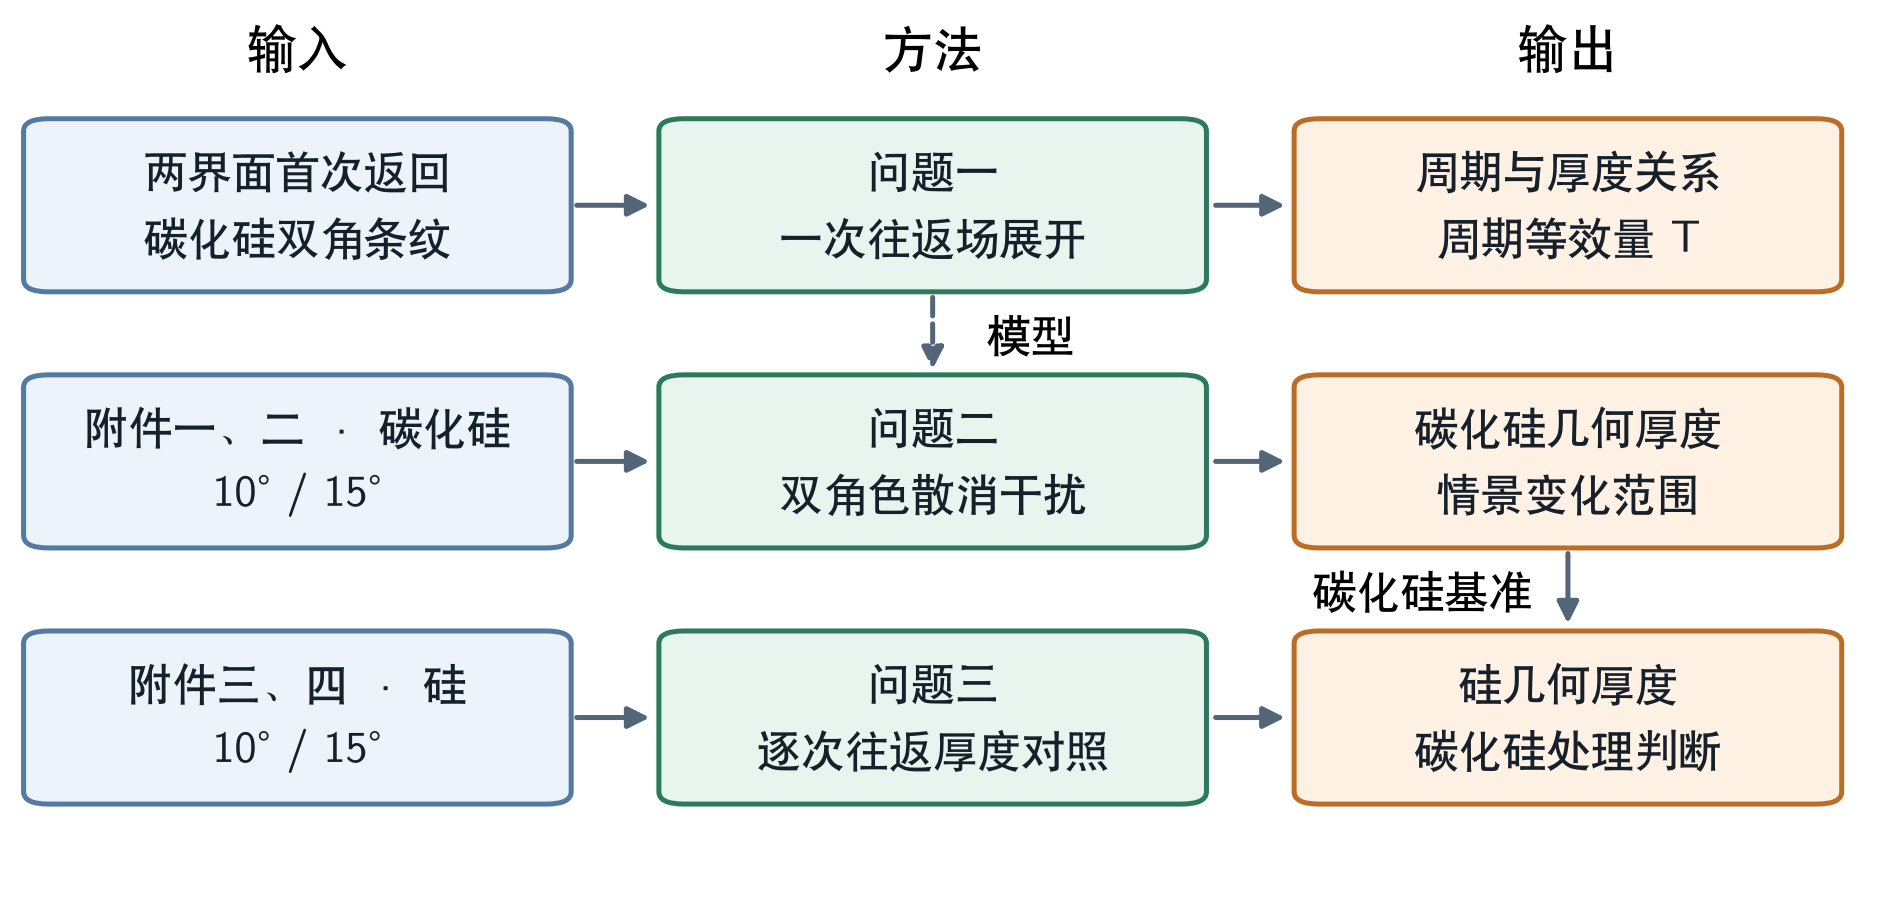
\includegraphics[width=0.8\textwidth,trim=0 38bp 0 0,clip]{../求解/公共/图片/全文思路图.png}
    \caption{四附件沿三问展开共同测厚路径}
    \label{fig:overall-route}
\end{figure}

总体组织吸收了高相关性的核对结果：两角原谱相关系数约为 $0.9987$，但来自同一块晶圆，并非独立厚度样本。原先以高相关性评价厚度可靠性的尝试，因而改为连续留段检验，即留出连续波段，用其观测检验双角预测。%
% src:交接/实验记录.json:50.现象;50.决定
% src:交接/数据档案.json:跨文件关系.两两全量核验.0.原始反射率皮尔逊相关系数

三问的结果按第\ref{sec:thickness-quantities}节的物理量定义区分；周期等效量为$19.54\ \mu\mathrm{m}$，表~\ref{tab:three-answers}将其与两种材料的测厚答案并列。%
% src:求解/问题1/结果/模型验证.json:真实附件诊断.表观光学厚度乘积_dq_微米

\begin{longtable}{>{\centering\arraybackslash}p{0.09\textwidth} >{\centering\arraybackslash}p{0.36\textwidth} >{\centering\arraybackslash}p{0.23\textwidth} >{\centering\arraybackslash}p{0.20\textwidth}}
\caption{三问回答的物理量与适用条件}\label{tab:three-answers}\\
\hline
问题 & 物理量 & 数值及单位 & 适用条件\\
\hline
\endfirsthead
\hline
问题 & 物理量 & 数值及单位 & 适用条件\\
\hline
\endhead
问题一 & 周期等效量 $T$ & $19.54\,\mu\mathrm{m}$ & 条纹周期折算\\
问题二 & 碳化硅几何厚度 & $10.80\,\mu\mathrm{m}$ & 非触边代表值\\
问题三 & 硅完整往返条件估计 & $2.17\,\mu\mathrm{m}$ & 给定经验色散\\
问题三 & 硅非概率条件包络 & $1.72$--$18.16\,\mu\mathrm{m}$ & 多情景联合范围\\
\hline
\end{longtable}
\nopagebreak[4]
\noindent{\small 注：硅点估计对应全量光谱；包络是多情景范围，不是置信区间。}
% src:求解/问题1/结果/模型验证.json:真实附件诊断.表观光学厚度乘积_dq_微米
% src:求解/问题2/结果/厚度结果.json:同片最佳厚度_微米;条件区间_微米
% src:求解/问题3/结果/回炉轮3候选/仲裁闭环/20260910_131501_81623_建模公式/厚度结果.json:核心指标.硅全量完整往返厚度_um;核心指标.碳化硅正式基准厚度_um
% src:求解/问题3/结果/回炉轮3候选/仲裁闭环/20260910_131501_81623_建模公式/厚度结果.json:核心指标.硅已计算条件包络下限_um;核心指标.硅已计算条件包络上限_um

碳化硅行采用透明两束与经验色散假设，代表值保留参数未碰到搜索边界的原估计。另有 $13.53\,\mu\mathrm{m}$ 的候选损失更低，但折射率已到搜索下界；分段重估、近优解及参数扰动构成的完整情景范围仍为 $0.64$--$18.11\,\mu\mathrm{m}$。
% src:求解/问题2/结果/厚度结果.json:同片最佳厚度_微米;同片最佳厚度的参考折射率;全量训练标准化损失;条件区间_微米;条件区间构造;条件区间组成
% src:求解/问题2/结果/验证.json:窗口与模型灵敏度.8.厚度_um;窗口与模型灵敏度.8.参考折射率;窗口与模型灵敏度.8.训练标准化损失
% src:求解/问题2/结果/搜索补查.json:代表点规则;补查最低损失候选.触边参数

周期等效量与几何厚度的换算条件统一见第\ref{sec:thickness-quantities}节。

入口、角度和结果对象被这样锁定后，后文即可先检查原始数据边界，再分别展开一次返回、双角估计与高阶往返的物理关系。

\section{数据审查与建模边界：保留原谱和未知条件}

上一章区分了周期等效量与拟合厚度，本章先核对支撑这些结果的原始光谱，再确定模型使用的观测范围。附件口径见表~\ref{tab:attachment-check}，共同坐标与拟合区段见附录图~\ref{fig:common-coordinate}。
% src:交接/数据档案.json:总览.附件总数;总览.独立晶圆数;总览.每块晶圆入射角度;跨文件关系.同片分组

异常原值遵循“标记、保留、单列影响”。附件二有262个超出反射率物理范围的原始值，集中在低波数端；图\ref{fig:raw-anomaly}和表\ref{tab:attachment-check}保留其位置与幅值。第一次尝试按物理范围裁剪，核对后改为保留原值，因为异常段与主拟合窗口不相交；保留或裁剪这些窗外点，主拟合窗口内的输入均相同。后文据此展开附件体检与参数缺口核对。
% src:交接/数据档案.json:总览.超过百分之百总点数;文件档案.1.工作表.0.字段档案.1.统计.最大值;文件档案.1.工作表.0.反射率检查.超过百分之百区段
% src:交接/实验记录.json:535.现象;535.决定
% src:交接/数据档案.json:未随附件提供的建模输入

\subsection{附件体检：共同坐标与异常原值}
\label{sec:common-coordinates}

共同首点和超界原值先定义了本节的边界：四谱的共同首点都是 $0\%$ 反射率，附件2另有262个超过 $100\%$ 的原始点，最高约为 $102.74\%$。图~\ref{fig:raw-anomaly}与表~\ref{tab:attachment-check}保留异常的位置与幅值；图中全谱与低波数端放大并列，异常被作为可见的数据事实保留，而不是静默改成缺失。
% src:交接/数据档案.json:总览.零反射率总点数
% src:交接/数据档案.json:总览.超过百分之百总点数;文件档案.1.工作表.0.字段档案.1.统计.最大值;文件档案.1.工作表.0.反射率检查.超过百分之百区段

\begin{figure}[H]
    \centering
    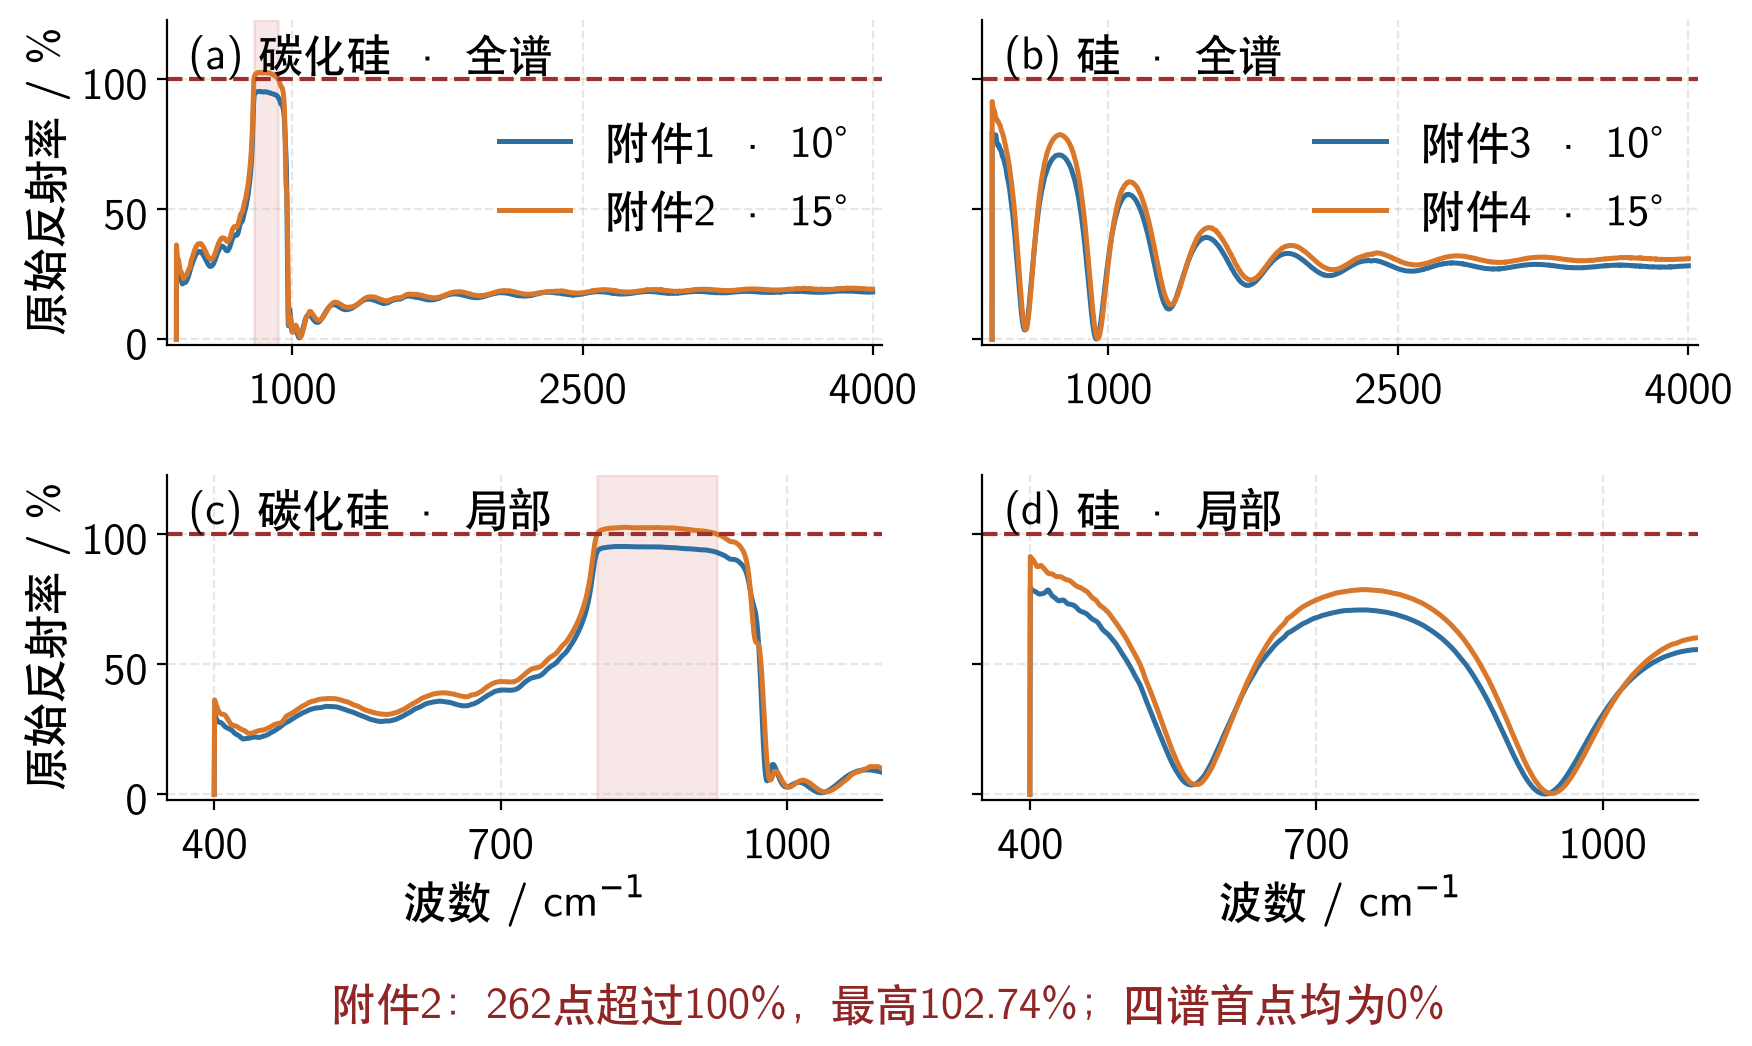
\includegraphics[width=0.96\textwidth]{../求解/公共/图片/四谱原值显示低波数异常.png}
    \caption{四谱原值在低波数端的异常分布}
    \label{fig:raw-anomaly}
\end{figure}

这些质量标记与坐标事实并列后，表~\ref{tab:attachment-check} 给出四谱进入后续比较前的统一口径。

\begin{longtable}{>{\centering\arraybackslash}p{0.20\textwidth}>{\centering\arraybackslash}p{0.24\textwidth}>{\centering\arraybackslash}p{0.24\textwidth}>{\centering\arraybackslash}p{0.20\textwidth}}
\caption{四谱附件体检摘要}\label{tab:attachment-check}\\
\hline
检查对象 & 共同事实 & 质量标记 & 处理口径 \\
\hline
\endfirsthead
\caption[]{四谱附件体检摘要（续）}\\
\hline
检查对象 & 共同事实 & 质量标记 & 处理口径 \\
\hline
\endhead
四谱共同坐标 & 7469点 & 399.67--4000.12~cm$^{-1}$ & 保留原坐标 \\
共同首点 & 4点；$0\%$ & 四谱同首波数 & 标记、保留 \\
附件2超界 & 262点；最高 $102.74\%$ & 801.28--927.11~cm$^{-1}$ & 标记、不裁 \\
主拟合窗口 & 1200--3800~cm$^{-1}$ & 与超界段无交集 & 单独说明 \\
\hline
\end{longtable}
% src:交接/数据档案.json:总览.四文件共有波数点数;总览.波数范围;总览.零反射率总点数
% src:交接/数据档案.json:总览.超过百分之百总点数;文件档案.1.工作表.0.字段档案.1.统计.最大值;文件档案.1.工作表.0.反射率检查.超过百分之百区段
% src:交接/实验记录.json:535.尝试;535.现象;535.决定

四谱各有7469个逐点一致的波数坐标，使双角比较无需插值；相邻步长略有差别，并非严格等间距。曾以端点等距坐标替代原始坐标，发现仍有坐标偏差，因此相位和峰距计算保留原始波数。共同坐标、拟合窗口与质量标记的对照见附录图~\ref{fig:common-coordinate}。
% src:交接/数据档案.json:总览.四文件共有波数点数;总览.波数范围
% src:求解/问题1/结果/实测输入核验.json:共同原始波数点数;波数范围_每厘米
% src:交接/实验记录.json:23.尝试;23.现象;23.决定



主拟合窗口是各模型共同使用的连续波段。低波数端的强烈起伏与中高波数条纹分段处理，高波数末端留作预测核对，主比较沿用原型的 $1200$--$3800\ \mathrm{cm}^{-1}$ 窗口。这两个端点是建模选择，并非裁剪超界点后形成的边界；其对测厚的影响由模型检验章的窗口移动比较考察。
% src:交接/计划.json:统一协议.连续留段.原型与正式区别;问题清单.1.验证方案.防泄漏.2
% src:交接/数据档案.json:文件档案.0.工作表.0.分波段描述
% src:交接/假设台账_问题2.json:5.假设;5.灵敏度义务;5.检验结果

比较按物理范围裁剪与保留原值两种口径后，发现异常段与主拟合窗口不相交，因而保留原始数值并单列质量标记。这里的标记注明异常的位置和幅值，窗外原值仍用于全谱展示与分波段统计。异常区段位于主拟合窗口之外，主拟合使用的原始数值未因此改变。
% src:交接/实验记录.json:535.尝试;535.现象;535.决定
% src:交接/图注素材_1.json:1.独有信息;3.独有信息

问题三的硅全量在同一窗口每角保留5392个原始点。
% src:求解/问题3/结果/解读核验_回炉3_仲裁后.json:防泄漏.全量每角点数

量纲也在此处锁定：反射率按百分数记录，计算按比例使用；波数保持 $\mathrm{cm}^{-1}$，厚度进入传播相位时用 $\mathrm{cm}$，输出再换成 $\mu\mathrm{m}$。因此，原值遵循“只标不裁”，坐标遵循“逐点对齐”；下一节据此检查不同波段的散布是否能够共用一个尺度，并核对光学参数缺口。
% src:交接/假设台账_问题1.json:1.假设

\subsection{可用信息：波段差异与光学参数缺口}
\label{sec:optical-inputs}

要判断哪些光谱变化能够进入后续测厚，先要确认全谱是否共享同一把尺度。

标准差衡量一段光谱内反射率围绕平均值的起伏大小。附件1的 $500$--$1000\ \mathrm{cm}^{-1}$ 波段反射率散布标准差约为 $28.9$ 个百分点。
% src:交接/数据档案.json:文件档案.0.工作表.0.分波段描述.1.左闭右开波数区间;文件档案.0.工作表.0.分波段描述.1.反射率统计.样本标准差

相较于低波数段，同一附件的 $3000$--$3500\ \mathrm{cm}^{-1}$ 波段标准差仅约为 $0.189$ 个百分点。这表明原始反射率的散布随波段明显变化，因此在相同窗口比较两角光谱；这里的标准差同时包含趋势与条纹，不用作测量噪声估计。图~\ref{fig:band-spread} 将四条光谱的分波段分布并置后，这一判断落在各段的整体形态上，而不是某一个孤立极值上。
% src:交接/数据档案.json:文件档案.0.工作表.0.分波段描述.1.反射率统计.样本标准差;文件档案.0.工作表.0.分波段描述.6.左闭右开波数区间;文件档案.0.工作表.0.分波段描述.6.反射率统计.样本标准差
% src:交接/图注素材_1.json:3.论文引用建议

\begin{figure}[H]
    \centering
    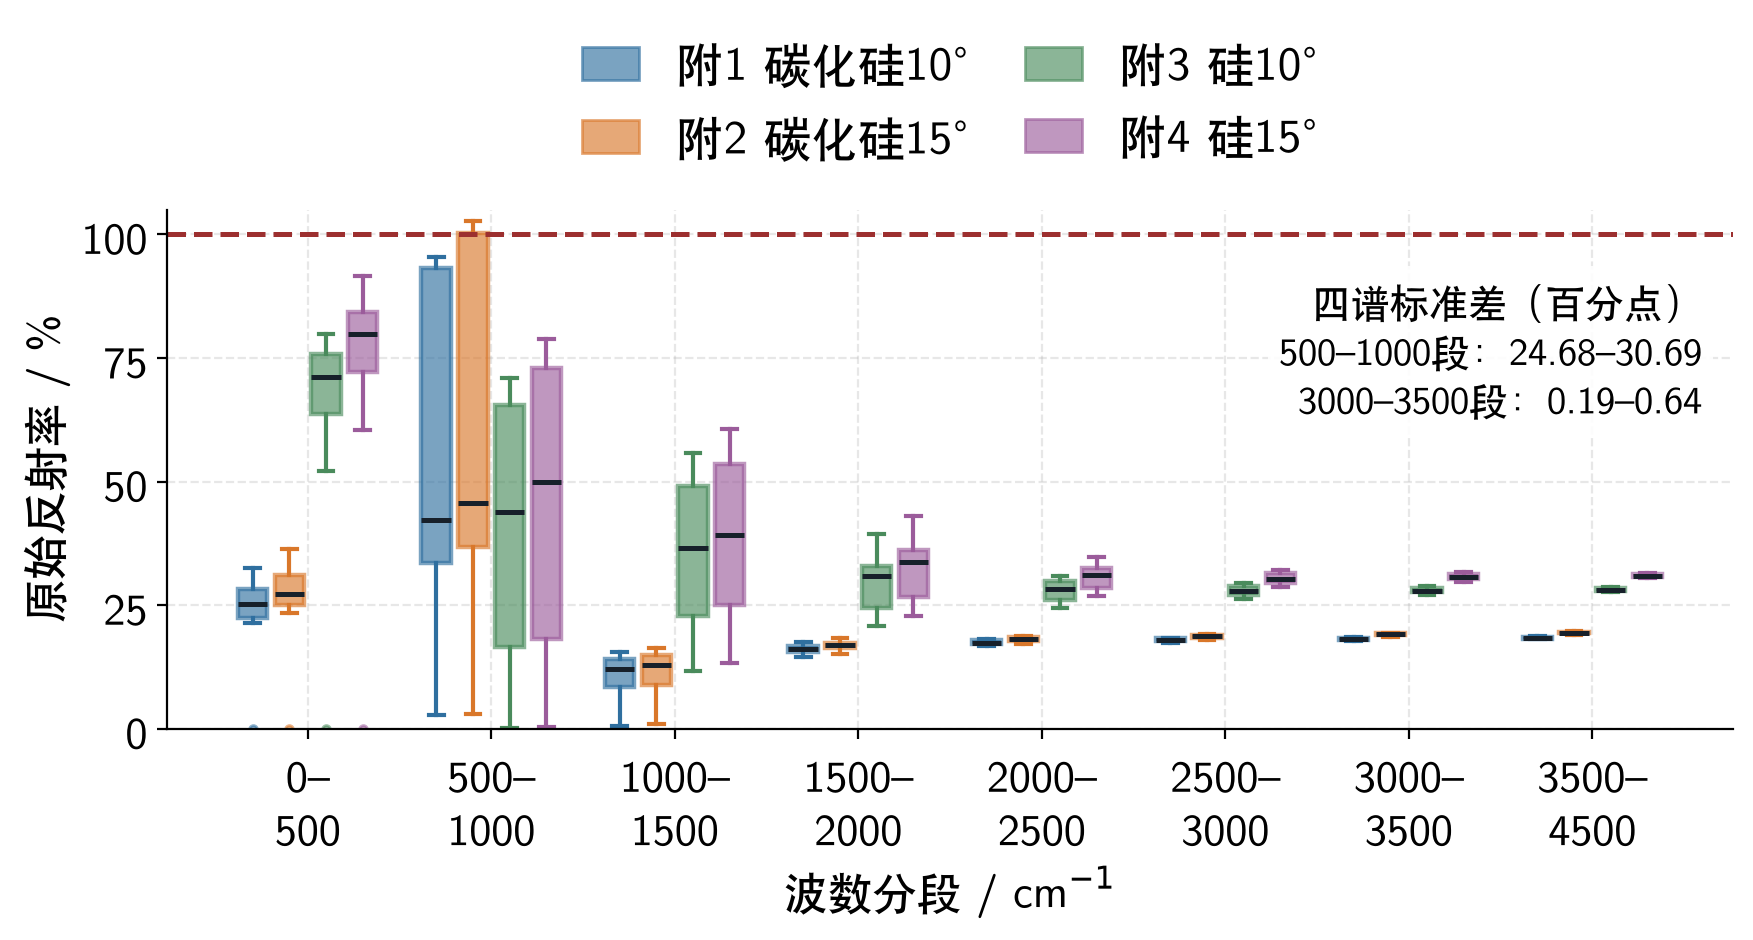
\includegraphics[width=0.96\textwidth]{../求解/公共/图片/波段散布差异不等于噪声.png}
    \caption{四谱低波数段反射率散布更大}
    \label{fig:band-spread}
\end{figure}

这种分段差异决定了选窗还须核对条纹连续性，并通过后文的窗口重估检查其影响。表~\ref{tab:available-info} 对照附件的材料与角度关系，原值保留规则沿用上一节。
% src:交接/数据档案.json:跨文件关系.同片分组;未随附件提供的建模输入

\begin{longtable}{>{\centering\arraybackslash}p{0.22\textwidth} >{\centering\arraybackslash}p{0.22\textwidth} >{\centering\arraybackslash}p{0.22\textwidth} >{\centering\arraybackslash}p{0.22\textwidth}}
\caption{附件与可用光学信息}\label{tab:available-info}\\
\hline
对象 & 材料与角度 & 原始规模与单位 & 标记或缺口\\
\hline
\endfirsthead
\hline
对象 & 材料与角度 & 原始规模与单位 & 标记或缺口\\
\hline
\endhead
附件1 & 碳化硅，$10^\circ$ & $7469$点；\(\mathrm{cm}^{-1}\)、\% & 超百值 $0$\\
附件2 & 碳化硅，$15^\circ$ & $7469$点；\(\mathrm{cm}^{-1}\)、\% & 超百值 $262$\\
附件3 & 硅，$10^\circ$ & $7469$点；\(\mathrm{cm}^{-1}\)、\% & 超百值 $0$\\
附件4 & 硅，$15^\circ$ & $7469$点；\(\mathrm{cm}^{-1}\)、\% & 超百值 $0$\\
共同缺口 & 两种材料，双角观测 & 仅有反射率与波数 & 五类输入缺失\\
\hline
\end{longtable}
% src:交接/数据档案.json:总览.四文件共有波数点数;总览.每块晶圆入射角度;跨文件关系.同片分组;文件档案.0.工作表.0.反射率检查.超过百分之百点数;文件档案.1.工作表.0.反射率检查.超过百分之百点数;文件档案.2.工作表.0.反射率检查.超过百分之百点数;文件档案.3.工作表.0.反射率检查.超过百分之百点数;未随附件提供的建模输入

坐标使用规则见第\ref{sec:common-coordinates}节，测厚还需要附件之外的光学信息。折射率曲线、消光系数、偏振状态、仪器分辨率和真实厚度均未给定；相干长度与光束空间重叠也缺少独立观测。前几项决定相位和反射强度如何换算为厚度，后两项关系到多次返回能否形成可观测干涉。
% src:交接/数据档案.json:未随附件提供的建模输入

初步核对固定折射率的同型峰距法时，上述标定缺口阻断了直接换算，因此将折射率变化显式保留在相位模型中。
% src:交接/实验记录.json:40.尝试;40.现象;40.决定

未标定的光学量将在下一章转为显式假设，并逐项说明其生效位置与检验方法。

\section{模型假设与符号说明：让光学条件可追溯}

本章把每项简化固定在它实际发生的建模位置，并给出可复核的检验。模型将空气、外延层和衬底分成三层，外部入射角取 $10^\circ$ 与 $15^\circ$；三层结构用于界面反射、透射和纵向传播因子的表达，分别由场展开互验、被动传播支检查和双角重估核对。
% src:交接/数据档案.json:总览.每块晶圆入射角度
% src:交接/假设台账_问题1.json:0.假设;0.检验结果
% 依据:交接/建模笔记_问题1.md:2. 几何、波数和传播因子

三问依次使用首个返回场、双角共享相位与完整往返场；透明近似、偏振权重和有效损耗的适用位置由假设表逐项限定。
% src:交接/假设台账_问题1.json:1.假设;1.检验结果
% src:交接/假设台账_问题2.json:3.假设;3.检验结果
% src:交接/假设台账_问题3.json:3.假设;3.检验结果;4.假设;4.检验结果;5.假设;5.检验结果

单位约定贯穿三问：反射率先按比例进入计算，波数以 $\mathrm{cm}^{-1}$ 记录，厚度在相位中以厘米计算，输出时再换算为微米。厚度沿 $8\,\mu\mathrm{m}\rightarrow0.0008\,\mathrm{cm}\rightarrow8\,\mu\mathrm{m}$ 回算一致，说明波数与厚度相乘的相位无量纲；下面两小节将把这些生效位置展开为假设表，并用统一符号承接三问的场模型。
% src:求解/问题1/结果/模型验证.json:单位换算.输入厚度_微米;单位换算.厚度_厘米;单位换算.回换厚度_微米

\subsection{模型假设：分层介质与有限信息}

本节先把光路放回实物：空气、外延层和衬底构成相邻的分层介质；假设的职责是规定波矢穿过界面、返回场保留阶数，以及缺失光学量由何种参数承接。本文采用非磁、标量、平面平行且层内均匀的介质近似。三层界面两侧沿界面方向的波矢分量连续，两种偏振采用同一套界面规则。导纳可理解为界面上电场与磁场关系的比例量；纵向传播因子把折射率与层内传播方向合在一起，透明时等于该层折射率乘以光线与垂直界面方向夹角的余弦。$s$偏振的电场垂直入射面，其导纳取纵向传播因子；$p$偏振的电场平行入射面，其导纳取该层折射率平方与纵向传播因子的比值，二者共同进入界面系数。空气折射率取$1$，外延层和衬底折射率仍按随波数变化的未知函数处理。表\ref{tab:02}把假设绑定到公式位置和核验方式。
% 依据:交接/建模笔记_问题1.md:1.题面边界与数据事实;2.几何、波数和传播因子;3.界面系数与一次往返场
% src:交接/假设台账_问题1.json:0.假设
\begingroup
\zihao{5}
\setlength{\tabcolsep}{3pt}
\begin{longtable}{>{\centering\arraybackslash}p{0.26\textwidth} >{\centering\arraybackslash}p{0.33\textwidth} >{\centering\arraybackslash}p{0.33\textwidth}}
\caption{模型假设的作用位置与核验方式}\label{tab:02}\\
\hline
假设 & 作用位置 & 核验方式\\
\hline
\endfirsthead
\hline
假设 & 作用位置 & 核验方式\\
\hline
\endhead
平面平行层 & 传播、界面系数 & 场表达式互核\\
被动传播 & 传播因子 & 衰减与单位回换\\
偏振加权 & 导纳、反射率 & 权重重估\\
经验色散 & 往返相位 & 常数与扰动对照\\
有效损耗 & 传播因子模长 & 损耗与收敛核对\\
逐问返回阶数 & 两束场、往返场 & 级数与闭式核对\\
允许观测偏差 & 灵敏度检验 & 保留原值重估\\
\hline
\end{longtable}
\endgroup

被动传播要求幅度沿光路不增长；偏振等权是加权模型中的一个情景。有效损耗合并吸收与界面造成的振幅衰减，避免把它拆成资料无法区分的来源。

场表达式互核比较直接计算的光场强度与交叉项展开式，核对两种写法的代数一致性；结构适用性则由生成光路与估计光路不同的失配情景检查。
% src:交接/假设台账_问题1.json:0.假设;0.灵敏度义务

界面规则确定后，返回阶数按题面逐问收紧。问题一把到达衬底界面后返回的首束记为$B$，把直接反射记为$r_{01}$，两束截断场记为$E_2$；问题三才允许后续每次往返再乘同一个往返复倍率$u$。这里的往返复倍率是光再绕一周时同时改变振幅和相位的因子，完整往返场记为$E_\infty$，其关系写成
\begin{equation}
E_2=r_{01}+B,\qquad E_\infty=r_{01}+B(1+u+u^2+\cdots)=r_{01}+\frac{B}{1-u},\qquad |u|<1 .
\end{equation}
其中$|u|<1$表示每增加一次往返，返回场的振幅就按小于一的倍率递减，需逐点检查，不由材料名称预设。该条件保证返回场级数收敛；高阶条纹能否观测，还取决于光束相干、空间重叠及测量分辨条件，问题三分别检查。具体而言，各束光须保持稳定的相位关系并落在同一探测区域，高阶条纹的变化还须能与噪声区分且能被仪器分辨。返回阶数固定后，色散承接相位变化，损耗承接传播振幅的衰减。
% 依据:交接/建模笔记_问题1.md:3.界面系数与一次往返场
% 依据:交接/建模笔记_问题3.md:2.从界面场到多次往返场;4.多光束必要条件及精度影响
% src:交接/假设台账_问题3.json:5.假设

损耗来源的处理来自一次参数化取舍：曾比较分项描述消光、界面损耗和偏振权重，与合并有效往返损耗两种方案。附件缺少分辨各损耗来源的独立观测，因而采用合并结构，折射率随波数的变化仍用少量参数描述。原始反射率允许存在测量偏差，异常值、选段和残差用于检查假设对厚度估计及光谱预测的影响。
% src:交接/实验记录.json:43.尝试;43.现象;43.决定
% src:交接/数据档案.json:未随附件提供的建模输入
% src:交接/假设台账_问题3.json:2.假设;3.假设;4.假设

这些约束把“采用什么假设”落实为“假设在哪一步生效、如何被扰动核对”；下一节据此统一外角、复折射率、相位因子以及厘米和微米的符号与量纲。

\subsection{符号说明：波数相位与厚度量纲}
\label{sec:thickness-quantities}

波数、角度和厚度必须先各自归位，才能让同一条相位关系在三问之间不换口径。真空波长记为 $\lambda_{\mathrm{vac}}$，$\sigma=1/\lambda_{\mathrm{vac}}$ 为波数，单位为 $\mathrm{cm}^{-1}$；题面给出的 $10^\circ$、$15^\circ$ 是空气侧外部入射角，记为 $\theta$，层内传播角记为 $\theta_j$。外部角度只负责界面入射条件，层内相位由纵向因子 $q_j$ 承接，不能把 $10^\circ$ 或 $15^\circ$ 直接代入层内相位。
% src:交接/数据档案.json:总览.每块晶圆入射角度
% 依据:交接/建模笔记_问题1.md:2. 几何、波数和传播因子

用 $j=0,1,2$ 标记空气、外延层和衬底，外延层几何厚度记为 $d$，相位计算取其厘米值 $d_{\mathrm{cm}}$。透明层内可写作 $q_j=N_j\cos\theta_j$，复折射率存在虚部时仍以根式定义的 $q_j$ 作为传播量。介质 $j$ 的复折射率写为 $N_j(\sigma)=n_j(\sigma)+i\kappa_j(\sigma)$，其中 $i$ 为虚数单位，于是
\begin{equation}
q_j(\sigma,\theta)=\sqrt{N_j(\sigma)^2-\sin^2\theta},\qquad
z(\sigma,\theta;d)=\exp\!\left(4\pi i\,d_{\mathrm{cm}}\sigma q_1(\sigma,\theta)\right).
\end{equation}
式中 $q_j$ 表示沿厚度方向的传播，根号取虚部非负的根，即 $\operatorname{Im}q_j\ge0$，透明介质取非负实根，使传播幅度不增长；虚部为正时光在传播中衰减。$z$ 表示光在外延层中往返一次后的复传播因子。这样，外部角度和层内传播方向被明确分开。
% 依据:交接/建模笔记_问题1.md:2. 几何、波数和传播因子

角度和波数统一后，还要把一次返回与完整往返场分成两个符号。令 $r_{jk}$、$t_{jk}$ 分别表示从介质 $j$ 到介质 $k$ 的复反射、透射系数；以下对每种偏振分别定义，省略偏振下标，入射场振幅归一为1。将表面直接反射加首个返回记为 $E_2$，将表面反射加全部往返记为 $E_\infty$，则
\begin{equation}
E_2=r_{01}+t_{01}t_{10}r_{12}z,\qquad
E_\infty=r_{01}+\frac{t_{01}t_{10}r_{12}z}{1-r_{10}r_{12}z}.
\end{equation}
其中 $E_2$ 只保留表面直接反射和首个返回，$E_\infty$ 才把后续返回写成几何级数；$d$ 始终表示外延层几何厚度，同片双角共享其值，硅与碳化硅分别估计。同一比较内两种场共用 $z$；问题三以实折射率和有效损耗参数化其相位与幅度。表~\ref{tab:03} 汇总符号含义、单位及双角共享或各角独有的用法。

\begingroup
\zihao{5}
\setlength{\tabcolsep}{3pt}
\begin{longtable}{>{\centering\arraybackslash}p{0.22\textwidth} >{\centering\arraybackslash}p{0.34\textwidth} >{\centering\arraybackslash}p{0.36\textwidth}}
\caption{符号含义、单位与角度用法}\label{tab:03}\\
\hline
符号 & 短含义 & 单位与使用属性\\
\hline
\endfirsthead
\hline
符号 & 短含义 & 单位与使用属性\\
\hline
\endhead
$j,\lambda_{\mathrm{vac}},\sigma$ & 层编号、真空波长、波数 & 无量纲、$\mathrm{cm}$、$\mathrm{cm}^{-1}$\\
$\theta,\theta_j$ & 外角、层内角 & 度；外角给定、内角求得\\
$N_j=n_j+i\kappa_j$ & 复折射率 & 无量纲；随材料、波数变化\\
$q_j,z$ & 纵向因子、往返因子 & 无量纲；随波数、外角变化\\
$\lambda$ & 有效往返损耗 & 无量纲；同片双角共享\\
$d_{\mathrm{cm}},d_{\mu\mathrm{m}}$ & 几何厚度 & 厘米、微米；同片共享\\
$r_{jk},t_{jk}$ & 复反射、透射系数 & 无量纲；随角度、偏振变化\\
$E_2,E_\infty$ & 两束场、完整往返场 & 无量纲；归一化复振幅\\
$\rho_{\%},R$ & 百分数反射率、反射率比例 & $R=\rho_{\%}/100$\\
\hline
\end{longtable}
\endgroup

表中 $N_j$ 的实部决定相位、虚部决定衰减；$q_j$ 描述纵向传播，$z$ 描述在外延层中的一次往返。$E_2$ 叠加表面反射与首个返回，$E_\infty$ 叠加表面反射与全部返回；$\lambda$ 用于问题三的有效往返损耗。

几何厚度$d$描述外延层上下界面的实际间距；周期等效量$T$则是把有限波段内拟合的条纹间距折算成的长度。令有效周期$\Delta\sigma$以$\mathrm{cm}^{-1}$计，$T$以$\mu\mathrm{m}$计，则
\begin{equation}
T=\frac{10^4}{2\Delta\sigma}.
\end{equation}
其中$\Delta\sigma$是整段光谱的周期统计量，不是每一对相邻条纹的局部间距。色散与界面相位的贡献均包含在条纹变化中；在透明近似下，只有这些变化足够小且相位在窗口内近似均匀变化时，$T$才近似为$d_{\mu\mathrm{m}}q_1$。这一区分使周期读数与外延层几何厚度各有明确对象，局部关系见式\eqref{eq:period-equivalent}。

厚度由厘米换为微米时，$d_{\mu\mathrm{m}}=10^4d_{\mathrm{cm}}$。
% src:求解/问题1/结果/模型验证.json:单位换算.输入厚度_微米;单位换算.厚度_厘米;单位换算.回换厚度_微米
这些符号固定了外角、层内传播与量纲，问题一据此推导表面反射和首个返回的合场强度。

\section{模型的建立与求解：从两束反射到逐次往返}

上一章统一了外角、纵向传播因子与厚度量纲，本章据此从一次返回场出发，将同片双角约束与后续往返逐步写入模型。图~\ref{fig:overall-route} 把这条关系画成同一条数据路径；问题一的两束边界和问题三的往返判据分别落在图\ref{fig:once-return}与图\ref{fig:roundtrip}中。返回阶数随题目需求逐层增加，一次返回先解释条纹，同片双角与完整往返场再分别处理两种材料。%
% src:交接/计划.json:叙事主线
% src:交接/论点脊柱.json:章.10.论点链.0.发现
% src:交接/图注素材_1.json:0.独有信息

三类验证量各有参照：问题一主方法的合成匹配平均误差为 $0.0008\%$，问题二连续留段标准化均方根误差为 $1.21$，问题三同口径误差为 $1.02$。前者衡量已知光学条件下的厚度回收，后两者分别衡量碳化硅与完整往返场的反射率预测表现。%
% src:求解/问题1/结果/合成验证.json:主指标.数值
% src:求解/问题2/结果/验证.json:正式主方法分数_连续留段标准化均方根误差
% src:求解/问题3/结果/回炉轮3候选/仲裁闭环/20260910_131501_81623_建模公式/厚度结果.json:分材料验证.硅.逐折汇总.0.平均标准化均方根误差.两束;分材料验证.硅.逐折汇总.0.平均标准化均方根误差.完整往返;分材料验证.硅.逐折汇总.0.平均标准化均方根误差.训练均值;分材料验证.硅.逐折汇总.0.平均标准化均方根误差.二次趋势;分材料验证.硅.逐折汇总.1.平均标准化均方根误差.两束;分材料验证.硅.逐折汇总.1.平均标准化均方根误差.完整往返;分材料验证.硅.逐折汇总.1.平均标准化均方根误差.训练均值;分材料验证.硅.逐折汇总.1.平均标准化均方根误差.二次趋势;分材料验证.碳化硅.逐折汇总.0.平均标准化均方根误差.两束;分材料验证.碳化硅.逐折汇总.0.平均标准化均方根误差.完整往返;分材料验证.碳化硅.逐折汇总.0.平均标准化均方根误差.训练均值;分材料验证.碳化硅.逐折汇总.0.平均标准化均方根误差.二次趋势;分材料验证.碳化硅.逐折汇总.1.平均标准化均方根误差.两束;分材料验证.碳化硅.逐折汇总.1.平均标准化均方根误差.完整往返;分材料验证.碳化硅.逐折汇总.1.平均标准化均方根误差.训练均值;分材料验证.碳化硅.逐折汇总.1.平均标准化均方根误差.二次趋势

结果关系随模型边界保留：问题二得到的 $10.80\ \mu\mathrm{m}$ 碳化硅拟合厚度，作为问题三继续比较时的碳化硅基准；硅则由完整往返场模型给出 $2.17\ \mu\mathrm{m}$ 的全量厚度估计。碳化硅的修正判断同时核对高阶返回的相干性、空间重叠和仪器分辨率，并比较同片厚度随场模型的变化。%
% src:求解/问题2/结果/厚度结果.json:同片最佳厚度_微米
% src:求解/问题3/结果/回炉轮3候选/仲裁闭环/20260910_131501_81623_建模公式/厚度结果.json:核心指标.碳化硅正式基准厚度_um;核心指标.硅全量完整往返厚度_um

双角原谱高相关曾被用来评价厚度可靠性，核对同片观测关系后，改用双角联动的连续留段检验评估共享参数。正文据此按问题一、问题二、问题三依次展开：先确定两束物理关系，再处理同片双角，最后比较完整往返场及其材料分支。%
% src:交接/实验记录.json:50.现象;50.决定

\subsection{问题一的建模与求解：一次往返场展开}

本问先回答条纹直接给出了什么量，再建立它与外延层厚度的联系。真实碳化硅光谱的周期等效量为$19.54\ \mu\mathrm{m}$，换算几何厚度还需光学参数。“一次往返场展开”是指：把外延层上表面的直接反射场，与光进入外延层、到达衬底界面后返回的首束场相加；光再次往返形成的更高阶返回不放入本问主模型。
% src:求解/问题1/结果/模型验证.json:真实附件诊断.表观光学厚度乘积_dq_微米

两谱有效周期约为$254.85$和$256.99\ \mathrm{cm}^{-1}$，以上述周期的中位数按第\ref{sec:thickness-quantities}节的定义折算。该实测量保留有限窗口内的色散和界面相位贡献，局部近似的条件由式\eqref{eq:period-equivalent}给出。
% src:求解/问题1/结果/模型验证.json:真实附件诊断.窗口_每厘米;真实附件诊断.周期投影诊断.0.周期_每厘米;真实附件诊断.周期投影诊断.1.周期_每厘米;真实附件诊断.表观光学厚度乘积_dq_微米

先限定为两束截断场，才能把角度、色散和偏振对条纹的作用逐项放入同一表达式，并把后续往返的收益单独检验；若直接引入高阶项，表面反射与首个返回的作用会失去清晰边界。两束的来源和真实数据的光学参数缺口将在分析与准备中交代，随后由界面导纳写出色散相位及其峰距关系。

\subsubsection{分析与准备：为何保留界面反射场}

本节先处理一个边界问题：问题一究竟应当把哪些返回光写进模型。条纹峰距只反映传播相位的变化，若折射率随波数变化而又没有标定，直接把峰距换成几何厚度就会把材料光学性质误当成厚度；因此主路线需要同时保留入射角、色散和偏振，而不是先填入一个固定折射率。

实测输入沿用第\ref{sec:common-coordinates}节的共同坐标，光学缺项见第\ref{sec:optical-inputs}节。两种角度改变了光线在外延层中的传播方向，却没有改变同片几何厚度；这使双角可以共同约束一条厚度参数，同时保留各自的界面振幅。直接采用全谱同型峰距并配固定折射率的尝试，正是因为这些输入缺失而被改为使用“波数乘纵向传播因子”的色散坐标。
% src:求解/问题1/结果/实测输入核验.json:共同原始波数点数;波数范围_每厘米
% src:交接/实验记录.json:26.现象;26.决定

两束边界由题面限定为表面直接反射和首个返回，后续往返不在本问提前叠加。图\ref{fig:once-return}把空气、外延层与衬底、外部入射角、层内传播方向和厚度路径放在同一几何关系中；所谓“双束界面场反演”，就是由这两束光的复场叠加计算反射率，再寻找使计算值与观测值接近的厚度。这样既保留了$10^\circ$与$15^\circ$的角度差异，也为问题三比较高阶返回留下清晰的基准。

\begin{figure}[H]
  \centering
  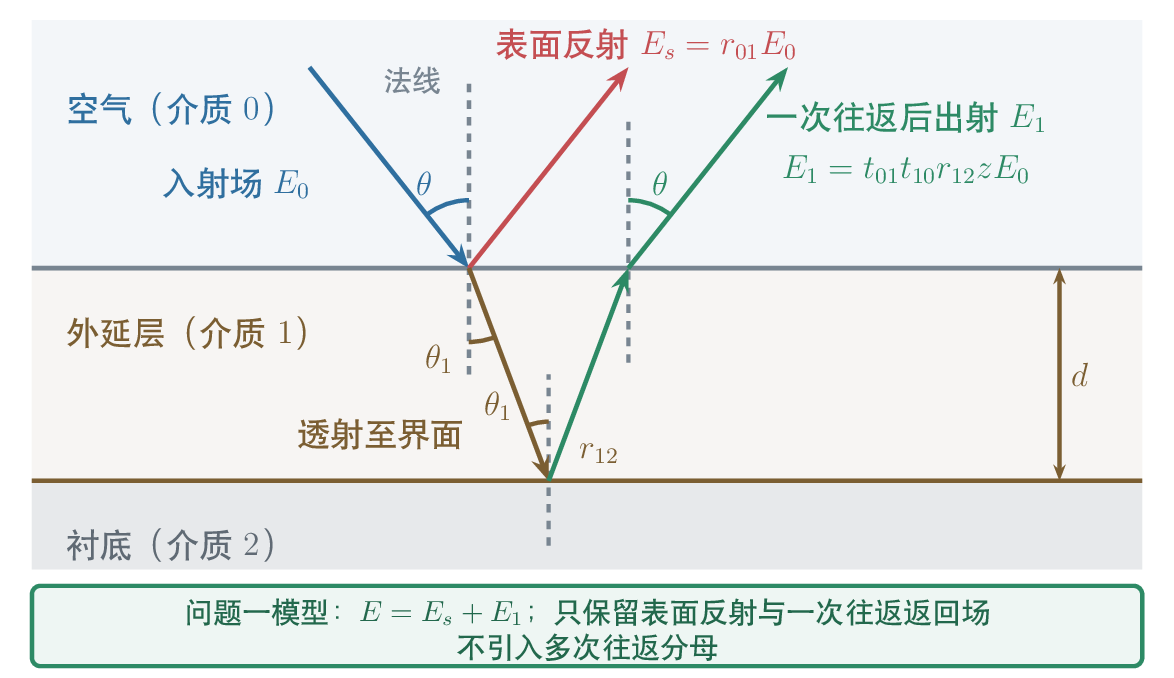
\includegraphics[width=0.8\textwidth]{../求解/问题1/图片/一次往返保留两束反射场.png}
  \caption{一次往返的两束反射场路径}
  \label{fig:once-return}
\end{figure}

路线选择也由同口径对照决定。已知光学参数的24组原型双角合成案例中，双束界面场反演的平均相对误差为$0.0010\%$，低于色散峰序反演的$0.0201\%$和连续相位拟厚的$0.0041\%$；逐观测输入一致的结论限定于这三个已核验原型，故没有把不同路线的结果平均，而是将后两者保留为级次与相位的独立核对。色散峰序反演按折射率变化修正峰谷位置，再按条纹级次求厚度；连续相位拟厚则沿波数展开条纹相位，由相位变化反推厚度。误差以合成光谱的已知厚度为参照，比较各路线在匹配生成机制下的回收表现。
% src:求解/问题1/原型结果/路线2.json:主指标值;已完成例数
% src:求解/问题1/原型结果/路线1.json:主指标值
% src:求解/问题1/原型结果/路线3.json:主指标值
% src:交接/锦标赛核验_问题1.json:共同输入核对
% src:交接/实验记录.json:66.现象;66.决定

正式复算另用一组生成观测，主方法平均误差为$0.0008\%$，与它使用相同输入的峰距基线为$2.59\%$；原型与正式组的含噪观测不同，二者不能拼成一组路线排名。
% src:求解/问题1/结果/合成验证.json:主指标.数值;常折射率峰距基线.平均绝对相对误差_百分比

强度形状进一步排除了“全谱恒幅条纹”的简化：附件1在$500$--$1000\ \mathrm{cm}^{-1}$和$3000$--$3500\ \mathrm{cm}^{-1}$两个诊断波段的反射率标准差分别为$28.9$和$0.189$个百分点，散布尺度相差悬殊。故主求解直接拟合两束截断场展开后的强度，局部极值和峰距承担相位解释与级次核对；下一节将从两束截断场推导偏振强度、色散相位及条纹间距。
% 依据:交接/建模笔记_问题1.md:4.强度展开、色散和峰谷系数
% src:交接/实验记录.json:27.现象;27.决定

\subsubsection{模型建立：色散相位决定条纹间距}

一次返回光谱的条纹来自两条路径的复场叠加：一条是外延层表面的直接反射，另一条是到达衬底界面后的首个返回。要让这两条路径同时承接本题的外部角度与波数，先把界面振幅和层内传播相位放在同一套符号中。

介质$j=0,1,2$依次为空气、外延层、衬底，外角为$\theta$，厚度$d$以$d_{\mathrm{cm}}=d$计算、以$d_{\mu\mathrm{m}}=10^4d_{\mathrm{cm}}$报告，波数为$\sigma$（$\mathrm{cm}^{-1}$），复折射率为$N_j=n_j+i\kappa_j$（实部$n_j$、消光系数$\kappa_j$），空气取$N_0=1$。平面界面上切向波矢守恒，归一化切向分量为$N_0\sin\theta=\sin\theta$，故纵向分量满足$N_j^2=q_j^2+\sin^2\theta$。层内纵向传播因子和一次往返传播因子定义为
\begin{equation}
q_j=\sqrt{N_j^2-\sin^2\theta},\qquad
z=\exp\!\left(4\pi i d_{\mathrm{cm}}\sigma q_1\right).
\end{equation}
其中$q_j$描述光在相应介质中沿厚度方向的传播，$z$则把外延层厚度、入射角和波数合并为一次往返的复相位；复根取$\operatorname{Im}q_j\geq0$，透明时取非负实根，使有损介质中的传播幅度不增长。
% 依据:交接/建模笔记_问题1.md:2.几何、波数和传播因子

偏振差异先进入界面导纳。记$s$、$p$为两种相互正交的偏振，$Y_j^{(a)}$为偏振$a$在介质$j$中的切向电场导纳。对任一偏振，在相邻介质$j,k$的界面处，把入射切向电场振幅归一为一，并将反射、透射振幅暂记为$r,t$；切向电场与磁场连续分别给出
\begin{equation}
1+r=t,\qquad Y_j(1-r)=Y_kt.
\end{equation}
这里$Y_j,Y_k$表示所选偏振在界面两侧的导纳。联立两式消去$t$求得$r$，再由$t=1+r$求透射系数；恢复偏振标记后有
\begin{equation}
Y_j^{(s)}=q_j,\qquad Y_j^{(p)}=\frac{N_j^2}{q_j},\qquad
r_{jk}^{(a)}=\frac{Y_j^{(a)}-Y_k^{(a)}}{Y_j^{(a)}+Y_k^{(a)}},\qquad
t_{jk}^{(a)}=\frac{2Y_j^{(a)}}{Y_j^{(a)}+Y_k^{(a)}}.
\end{equation}
这里$r_{jk}^{(a)}$和$t_{jk}^{(a)}$分别是从介质$j$到介质$k$的反射、透射振幅系数。令表面直接反射项$a_a=r_{01}^{(a)}$，首个返回的界面项$b_a=t_{01}^{(a)}t_{10}^{(a)}r_{12}^{(a)}$，题面的一次返回边界便给出
\begin{equation}
E_a=a_a+b_a z .
\end{equation}
因此，$s$、$p$偏振的差别留在$a_a,b_a$中，厚度则只通过$z$进入；$10^\circ$与$15^\circ$两条观测支路可以共享$d$，同时保留各自的界面响应。场表达式确定后，下一步是把正交偏振的强度混合，并展开其中的交叉干涉项。
% 依据:交接/建模笔记_问题1.md:3.界面系数与一次往返场

设$s$偏振强度权重为$w$，$0\leq w\leq1$，$p$偏振权重为$1-w$。由于两种偏振正交，观测反射率比例是两种偏振强度的加权和，而不是把两种电场直接相加。令$w_s=w$、$w_p=1-w$，并定义
\begin{equation}
U=\sum_a w_a|a_a|^2,\qquad V=\sum_a w_a|b_a|^2,\qquad C=\sum_a w_a a_a^*b_a,
\end{equation}
则一次返回模型的强度展开为
\begin{equation}
R_2=\sum_a w_a|E_a|^2=U+V|z|^2+2\operatorname{Re}(Cz).
\end{equation}
其中$U$是直接反射背景，$V|z|^2$是首个返回的幅度项，$2\operatorname{Re}(Cz)$是两条路径相遇产生的条纹项。
% 依据:交接/建模笔记_问题1.md:4.强度展开、色散和峰谷系数

两种强度写法在已知条件的合成光谱上相符；这里的合成光谱，是先给定厚度、折射率曲线与偏振比例，再由两束光相加生成的光谱。表\ref{tab:field-check-conditions}列出数值核对的条件，直接复场强度与交叉项展开的最大绝对差为$1.7\times10^{-16}$（反射率比例）；另令衬底与外延层折射率相同，在零返回核对点保留与去掉返回项的反射率差为$0$。
% src:求解/问题1/结果/模型验证.json:场展开一致性最大绝对差_比例;零界面返回项差_比例

\begingroup
\setlength{\tabcolsep}{0.01\textwidth}
\Needspace{11\baselineskip}
\begin{longtable}{>{\centering\arraybackslash}p{0.26\textwidth}>{\centering\arraybackslash}p{0.70\textwidth}}
  \caption{两种强度写法的数值核对条件}\label{tab:field-check-conditions}\\
  \toprule
  核对项目 & 取值 \\
  \midrule
  几何厚度 & $3,8,20\ \mu\mathrm{m}$ \\
  外部入射角 & $10^\circ,15^\circ$ \\
  波数采样 & 附件1原始坐标每隔$32$点取一点 \\
  外延层折射率 & $n_1(\sigma)=2.8+0.08(\sigma-2200)/1800$ \\
  衬底折射率 & $n_2(\sigma)=n_1(\sigma)+0.8$ \\
  吸收与偏振 & $\kappa_1=\kappa_2=0,\quad w=0.5$ \\
  零返回核对点 & $d_{\mu\mathrm{m}}=8,\quad\theta=10^\circ,\quad\sigma=2199.9\ \mathrm{cm}^{-1}$ \\
  \bottomrule
\end{longtable}
\endgroup
% 依据:求解/问题1/求解_问题1.py:model_validation;index_at
% src:数据/问题1_冻结合成输入/合成设计.json:基础情景.厚度_微米;角度_度;基础情景.垂直偏振权重;基础情景.衬底折射率增量;基础情景.消光系数;灵敏度锚例.折射率基值;灵敏度锚例.色散斜率;生成规则.归一化波数;生成规则.层折射率

附录图~\ref{fig:field-expansion}进一步交叉比较折射率基值为$2.4$或$3.4$、色散斜率为$0$或$0.08$的组合，厚度、角度、衬底折射率增量与偏振设置沿用表中的一般核对条件。散点贴近等值线，表示两种写法在同一波数点给出相同的反射率，而不是比较不同波数点的光谱形状。
% src:数据/问题1_冻结合成输入/合成设计.json:基础情景.折射率基值;基础情景.色散斜率;基础情景.厚度_微米;角度_度;基础情景.衬底折射率增量;基础情景.垂直偏振权重
% src:交接/图注素材_1.json:5.独有信息



两种强度写法的代数一致性确定后，进一步考察色散对条纹位置的作用。透明且包络变化较慢时，令$\psi=\arg C$，主干相位可写为
\begin{equation}
\Phi(\sigma,\theta)=4\pi d_{\mathrm{cm}}\sigma\operatorname{Re}q_1+\psi,\qquad
\Phi'=4\pi d_{\mathrm{cm}}\left(q_1+\sigma\frac{dq_1}{d\sigma}\right)+\frac{d\psi}{d\sigma}.
\end{equation}
式中撇号表示对波数$\sigma$求导。若折射率实部记为$n(\sigma)$，则$q_1=\sqrt{n^2-\sin^2\theta}$且$\mathrm{d}q_1/\mathrm{d}\sigma=nn'/q_1$，所以相位导数中的色散贡献为$\sigma nn'/q_1$。这一步把“条纹间距”落到相位对波数的变化率，而不是把一个全谱固定系数直接当成厚度。
% 依据:交接/建模笔记_问题1.md:4.强度展开、色散和峰谷系数

相位级次与反射率峰谷之间还隔着背景和振幅的变化。把强度展开整理为
\begin{equation}
R_2=B+A\cos\Phi,\qquad
R_2'=B'+A'\cos\Phi-A\Phi'\sin\Phi.
\end{equation}
其中$B=U+V|z|^2$为反射率背景，$A=2|Cz|$为条纹振幅。只有$A$不接近零，且$|B'|$、$|A'|$远小于$|A\Phi'|$时，反射率极值才近似对应相位级次。上一节的波段包络差异表明，全谱背景和振幅并不恒定，因此峰距承担局部相位核对，主求解仍拟合两束截断场强度。
% 依据:交接/建模笔记_问题1.md:4.强度展开、色散和峰谷系数

\begin{samepage}
在上述缓变条件下，相邻同型极值的相位差近似为一个完整周期，故其波数差$\Delta\sigma$满足
\begin{equation}
2d\,\Delta(\sigma q_1)+\frac{\Delta\psi}{2\pi}\simeq1,\qquad
d_{\mu\mathrm{m}}\simeq\frac{5000\left(1-\Delta\psi/(2\pi)\right)}{\Delta(\sigma q_1)}.
\end{equation}
\end{samepage}
对实际相邻同型条纹，将波数差记为$\Delta\sigma_{\mathrm{loc}}$，相应局部周期等效量记为$T_{\mathrm{loc}}$。将同型条纹关系除以该波数差，得到
\begin{equation}
\begin{aligned}
T_{\mathrm{loc}}&=\frac{5000}{\Delta\sigma_{\mathrm{loc}}}\simeq
d_{\mu\mathrm{m}}\frac{\Delta(\sigma q_1)}{\Delta\sigma_{\mathrm{loc}}}
+\frac{2500}{\pi}\frac{\Delta\psi}{\Delta\sigma_{\mathrm{loc}}},\\
T_{\mathrm{loc}}-d_{\mu\mathrm{m}}q_1&\simeq
d_{\mu\mathrm{m}}\frac{\sigma nn'}{q_1}+\frac{2500}{\pi}\psi'.
\end{aligned}
\label{eq:period-equivalent}
\end{equation}
这里差商表示相邻同型条纹间的平均相位变化，第二行为局部近似，右端给出偏离厚度乘纵向传播因子的两项来源。两项均可忽略时才有$T_{\mathrm{loc}}\simeq d_{\mu\mathrm{m}}q_1$。实测$T$来自有限窗口的最佳正弦周期，不等于逐点测得的$T_{\mathrm{loc}}$；将前者也简写为$dq_1$，还须核验窗口内相位斜率近似恒定。本题没有估计或扣除这些导数项，因而保留$T$作为周期统计量，不作厚度乘积的实测标定。

峰到谷只跨过半个周期，必须改写为
\begin{equation}
2d\,\Delta(\sigma q_1)+\frac{\Delta\psi}{2\pi}\simeq\frac12,\qquad
d_{\mu\mathrm{m}}\simeq\frac{2500\left(1-\Delta\psi/\pi\right)}{\Delta(\sigma q_1)}.
\end{equation}
当$n'=0$、界面相位变化缓慢且包络导数相对主相位项可忽略时，才退化为$5000/(q_1\Delta\sigma)$和$2500/(q_1\Delta\sigma)$。两个系数相差一倍，正是峰谷不能直接套用同型峰距式的原因；图\ref{fig:dispersion-spacing}进一步把色散斜率与波数对常数峰距偏差的共同作用分开显示。
% src:求解/问题1/结果/模型验证.json:常折射率退化.同型系数_微米;常折射率退化.峰谷系数_微米
% src:交接/实验记录.json:477.现象;477.决定
% 依据:交接/建模笔记_问题1.md:4.强度展开、色散和峰谷系数



峰谷系数的分开处理并非形式上的修补。奇偶级次反演在色散坐标中区分同型极值与半周期事件，同型极值不足时未用峰谷混合补足；全部合成案例均保留。因此本节保留两类级次的不同方程。
% src:交接/实验记录.json:56.尝试;56.现象;56.决定

固定光学条件后搜索得到的厚度解构成厚度候选，优劣以两角反射率的联合残差平方均值衡量，而不是预先给定干涉级次。相位坐标由此解释双角条纹疏密，并为下一节的合成回收、实测周期提取和低残差厚度候选提供共同依据。
% 依据:交接/建模笔记_问题1.md:5.厚度反演与验证方案

\subsubsection{求解与结果分析：合成回收与相位歧义}

色散相位已经解释条纹位置，本节进一步回答这条关系能否把厚度回收到正确分支，并把合成条件、真实光谱和方法边界分开。求解时以双角联合的两束界面场为主线，峰序与连续相位只承担结构核对。

在生成机制与反演机制一致的共同合成情景中，双束界面场反演的平均绝对相对误差为$0.0008\%$，同一输入下的常折射率峰距基线为$2.59\%$。在相同合成输入上，双束界面场反演的厚度回收误差低于常折射率峰距基线。
% src:求解/问题1/结果/合成验证.json:主指标.数值;常折射率峰距基线.平均绝对相对误差_百分比

因为这里要检验厚度反演本身，正式双束复算把膜层与衬底的折射率、消光系数及偏振权重固定为给定情景，只估计两角共享的厚度。联合损失就是模型反射率与观测反射率之差的平方在两角全部采样点上取平均，比较对象是反射率，而非电场或相位。每角按均匀索引向下取整选取$256$个原始波数坐标，厚度在$0.5$--$40\ \mu\mathrm{m}$内搜索；这个范围是算法搜索域，不是由观测推得的概率区间。
% src:数据/问题1_冻结合成输入/合成设计.json:坐标来源.使用点数_每角
% src:交接/算法参数核对_G4.json:问题一.厚度搜索范围_微米
% src:交接/假设台账_问题1.json:2.假设;3.假设
% 依据:交接/建模笔记_问题1.md:第5节“厚度反演与验证方案”

粗扫先比较$129$个等距厚度点，再对损失最低的$4$个候选作黄金分割精化，逐步缩小候选附近区间，最后取损失最小者。合成真厚度仅参与光谱生成和误差评分，搜索过程依据观测反射率选择候选。连续相位拟厚沿波数展开条纹相位，由相位变化反推厚度，并与场模型相互核对相位级次。
% src:交接/算法参数核对_G4.json:问题一.粗网格点数;问题一.精化候选数
% 依据:交接/建模笔记_问题1.md:第5节“厚度反演与验证方案”

共同案例全部保留，表\ref{tab:04}分列“原型三路线共同24例”与“正式双束复算共同24例”：案例集相同，配置不同，误差分别计算；破折号表示相应配置下未运行该路线。图中的原型逐例点对应前一行，正式复算的双束误差与常折射率峰距基线则配在后一行。
% src:求解/问题1/结果/合成验证.json:主指标.含义;分组汇总.共同匹配.案例数
% src:求解/问题1/原型结果/路线2.json:口径说明.搜索
% src:交接/实验记录.json:66.尝试;66.决定

逐例复核发现，连续相位路线在一个案例中同时保留了$3.0000\ \mu\mathrm{m}$与$36.8799\ \mu\mathrm{m}$两个候选；这里的相位歧义，是不同厚度都通过了相位拟合的候选筛选。计分采用相位回归残差较小的前一个厚度，另一个候选及歧义标记也保留，因此表中平均误差衡量的是所选主候选的回收程度。依据这项全案例核对，双束界面场被选作主方法，峰序与连续相位继续承担独立对照。
% src:求解/问题1/原型结果/路线3.json:合成逐例.0.求解.近优候选厚度_微米;合成逐例.0.求解.厚度_微米;合成逐例.0.求解.候选.0.相位回归均方根残差_弧度;合成逐例.0.求解.候选.1.相位回归均方根残差_弧度;辅助诊断.有歧义案例数
% src:交接/实验记录.json:66.类别;66.尝试;66.现象;66.决定

\begingroup
\small
\begin{longtable}{>{\centering\arraybackslash}p{0.28\textwidth}>{\centering\arraybackslash}p{0.06\textwidth}>{\centering\arraybackslash}p{0.12\textwidth}>{\centering\arraybackslash}p{0.11\textwidth}>{\centering\arraybackslash}p{0.10\textwidth}>{\centering\arraybackslash}p{0.13\textwidth}}
\caption{三路线与朴素基线的合成厚度误差}\label{tab:04}\\
\toprule
情景 & 例数 & 双束场/\% & 峰序/\% & 相位/\% & 峰距基线/\% \\
\midrule
原型三路线共同 & 24 & 0.0010 & 0.0201 & 0.0041 & -- \\
正式另组共同输入 & 24 & 0.0008 & -- & -- & 2.59 \\
新增匹配 & 16 & 0.0011 & -- & -- & -- \\
模型失配 & 10 & 0.3028 & -- & -- & -- \\
\bottomrule
\end{longtable}
\endgroup
% src:求解/问题1/原型结果/路线1.json:主指标值
% src:求解/问题1/原型结果/路线2.json:主指标值
% src:求解/问题1/原型结果/路线3.json:主指标值
% src:求解/问题1/结果/合成验证.json:分组汇总.共同匹配.案例数;分组汇总.新增匹配.案例数;分组汇总.模型失配.案例数;分组汇总.共同匹配.平均绝对相对误差_百分比;分组汇总.新增匹配.平均绝对相对误差_百分比;分组汇总.模型失配.平均绝对相对误差_百分比;常折射率峰距基线.平均绝对相对误差_百分比

共同案例的低误差并没有延伸到所有生成条件。新增匹配的$16$例扩展了厚度、折射率、色散斜率与曲率、偏振和噪声组合，生成与反演仍使用同一光学关系；其中折射率基值改为$2.8$和$3.1$，噪声标准差最高为$0.0015$（反射率比例）。这组案例检验的是改变参数后能否继续回收厚度。
% src:求解/问题1/结果/合成验证.json:分组汇总.新增匹配.案例数
% src:数据/问题1_冻结合成输入/合成设计.json:新增匹配情景

曲率和包络系数采用统一的波数尺度：把原波数减去$2200\ \mathrm{cm}^{-1}$再除以$1800\ \mathrm{cm}^{-1}$，得到无量纲的归一化波数。
% src:数据/问题1_冻结合成输入/合成设计.json:生成规则.归一化波数

模型失配则指生成光谱包含反演时遗漏或误设的成分。失配组共$10$例，包括遗漏$\pm0.12$的色散曲率、将$0.2$的垂直偏振权重按$0.5$求解等情景，图\ref{fig:08}分区比较参数变化与模型缺项的误差。
% src:求解/问题1/结果/合成验证.json:分组汇总.模型失配.案例数
% src:数据/问题1_冻结合成输入/合成设计.json:失配情景.0.生成曲率;失配情景.6.生成曲率;失配情景.1.生成权重;基础情景.垂直偏振权重
% src:交接/图注素材_2.json:0.图题;0.独有信息

其他失配还包括遗漏系数为$\pm0.05$的线性包络、系数为$0.01$的二次基线、消光系数为$0.002$的吸收，以及生成端含$8$束返回而反演仍按一次返回处理；包络与基线以归一化波数为自变量。部分案例同时改变两项，失配组均值因此反映这一组设定的综合影响。
% src:数据/问题1_冻结合成输入/合成设计.json:失配情景.2.生成增益;失配情景.7.生成增益;失配情景.3.生成基线;失配情景.4.生成消光系数;失配情景.5.生成返回束数;生成规则.归一化波数

\begin{figure}[H]
  \centering
  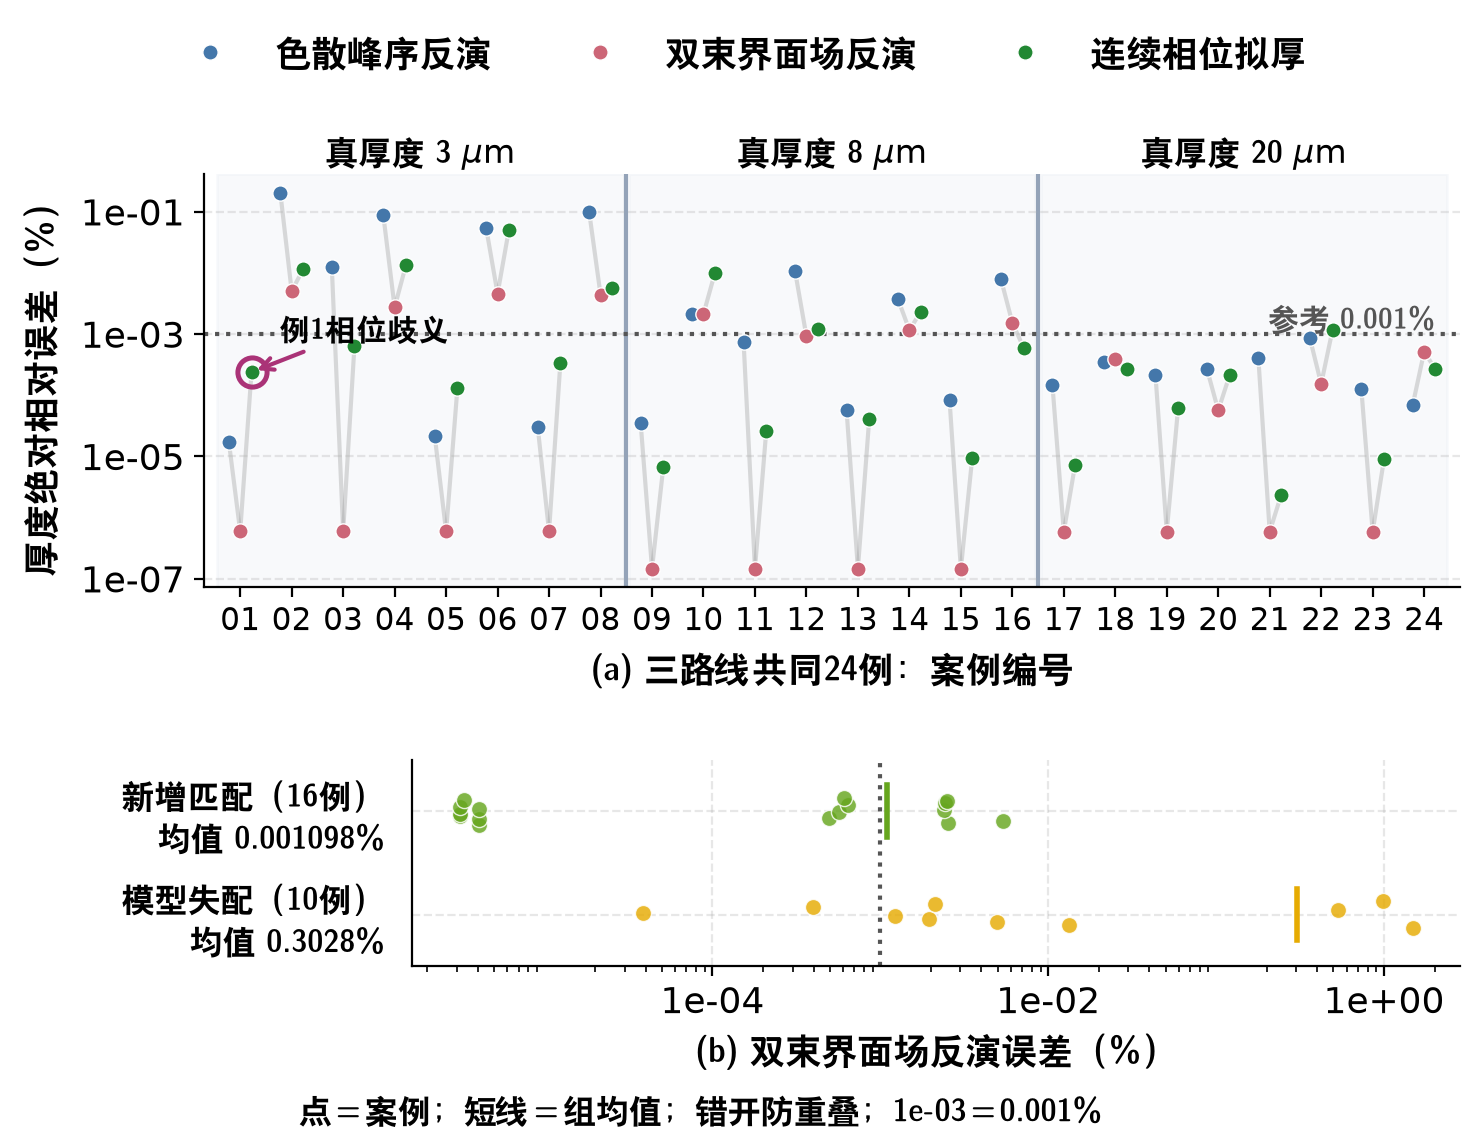
\includegraphics[width=0.96\textwidth]{../求解/问题1/图片/三路线误差按情景分布.png}
  \caption{三路线共同案例与失配情景误差}
  \label{fig:08}
\end{figure}

图\ref{fig:08}下部仅展示主方法在新增匹配与模型失配情景中的误差。上部是原型三路线在共同案例上的逐例配对，对应表\ref{tab:04}的原型行。另将一个角度整谱用于估计厚度，另一个角度整谱用于检验预测，再互换两角，称为两角互换验证；其厚度预测平均绝对相对误差为$0.0018\%$，说明角度互换后的方向性核对与共同案例结论一致。
% src:求解/问题1/结果/独立角度切分验证.json:留出指标.留出厚度预测平均绝对相对误差_百分比;切分原则
% src:交接/图注素材_2.json:0.图题;0.独有信息

保持按$8\ \mu\mathrm{m}$厚度生成的同一组合成观测不变，调整折射率、偏振、平滑宽度和入射角后重估，厚度为$6.66$--$10.01\ \mu\mathrm{m}$。这一厚度重估范围记录同一合成样本对设定变化的响应，比较时固定观测，以分开输入变化与估计条件变化的作用。
% src:数据/问题1_冻结合成输入/合成设计.json:灵敏度锚例.厚度_微米
% src:求解/问题1/结果/灵敏度.json:条件压力范围_微米;范围含义

真实光谱的周期提取先处理缓慢变化的背景。在$2800$--$3600\ \mathrm{cm}^{-1}$窗口内，将反射率与候选周期的正余弦列投影到同一二次基线并取残差，扣除慢变背景后搜索最能解释振荡的周期。
% src:求解/问题1/结果/模型验证.json:真实附件诊断.窗口_每厘米;真实附件诊断.周期投影诊断.0.基线与谐波口径;真实附件诊断.周期投影诊断.1.基线与谐波口径

两谱提取的周期分别为$254.85$和$256.99\ \mathrm{cm}^{-1}$，将两周期的中位数代入定义式得到$T=19.54\ \mu\mathrm{m}$。这里报告的是有限窗口周期统计量；色散和界面相位贡献未被分离，不能直接解释为$dq_1$或几何厚度。式\eqref{eq:period-equivalent}约束的是实际相邻条纹的局部差商，不能把其中的近似条件当作本次窗口拟合已经验证的结论。
% src:求解/问题1/结果/模型验证.json:真实附件诊断.周期_每厘米;真实附件诊断.表观光学厚度乘积_dq_微米

问题一的结论为：双束界面场反演在固定合成条件下的平均回收误差为$0.0008\%$，优于峰距基线的$2.59\%$，实测周期等效量为$T=19.54\ \mu\mathrm{m}$。
% src:求解/问题1/结果/合成验证.json:主指标.数值;常折射率峰距基线.平均绝对相对误差_百分比
% src:求解/问题1/结果/模型验证.json:真实附件诊断.表观光学厚度乘积_dq_微米

本问置信等级为低：周期等效量有独立复算支持，合成回收、常折射率基线比较与两角互换验证支持方法选择。真实附件缺少折射率、消光系数、偏振状态和厚度真值，厚度重估范围较宽，周期等效量尚未换算为标定后的几何厚度。合成误差衡量给定光学条件下的厚度回收，不代表真实晶圆的测量精度。
% src:交接/结果声明_问题1.json:置信.等级;置信.理由

由此，下一问需要利用同片双角的共同信息进一步压缩未知光学因素，把周期等效量推进到可比较的给定光学条件下的厚度。

\subsection{问题二的建模与求解：双角色散消干扰}

两条碳化硅光谱来自同一块晶圆，逐行共享$7469$个波数点，却有$2.14$个百分点的反射率均方根差；这意味着厚度应当共享，基线、振幅和相位却不能把两角硬压成一条曲线。双角色散消干扰据此把共同的条纹位置交给厚度与色散，把角度特有的慢变响应留在各自的有限参数中，而不是将两角原谱先平均。
% src:交接/数据档案.json:跨文件关系.同片分组
% src:交接/数据档案.json:跨文件关系.两两全量核验

全量同片拟合给出$10.80\ \mu\mathrm{m}$的拟合厚度；五折连续留段显示厚度分支明显漂移，因此谱形解释与厚度辨识并列呈现。正式留段标准化均方根误差为$1.21$，相对二次趋势基线改善$16.2\%$，说明条纹项增加了模型对留出反射率的解释力。
% src:求解/问题2/结果/厚度结果.json:同片最佳厚度_微米
% src:求解/问题2/结果/验证.json:正式主方法分数_连续留段标准化均方根误差;正式主方法相对正式二次趋势改善_百分比

这条主线把“共享厚度”与“角度响应”分成两个层次，下面依次给出分块准备、共同厚度投影模型及其结果边界。

\subsubsection{分析与准备：分块观测与受限干扰项}

问题二要在同一块晶圆的两条光谱中找出共同的厚度信息，同时把入射角造成的外观差异留在各自模型里。为避免相邻波数点被误当成独立测试，先把主拟合窗口的原始坐标组织成连续区段，再分别安排估计、校准与计分。在$1200$--$3800\ \mathrm{cm}^{-1}$主拟合窗口内，先按波数升序排列观测，再将首末观测之间的序号范围均分为$479$份，分点序号向下取整，连同两端共取$480$个原始坐标点；保留附件给出的波数值，不插值为等距波数网格。
% src:求解/问题2/结果/数据审查.json:主窗口_cm^-1;抽样点数_每角度;抽样索引

这些坐标按顺序每$40$点组成一块，形成$12$个连续块，块号随波数递增。连续块数和训练边界的$20\ \mathrm{cm}^{-1}$保护带均由两角共同使用并预先固定，保护带隔开邻近观测以减轻信息串入。
% src:求解/问题2/结果/数据审查.json:抽样索引
% src:求解/问题2/结果/基准交接.json:训练保护带_cm^-1;折分

训练段估计参数并确定归一化尺度，校准段只校准预测区间半宽，测试段只计分。正式比较采用两折，即两套训练、校准和测试的区段分工，具体块号见表\ref{tab:05}；上一节的五折是在同一组连续块上另行轮换测试区段，用于检查厚度随留段位置的变化，并非另分五个块。图\ref{fig:split}展示两角采用相同波数分组的两折训练、校准和测试安排；这种安排使模型选择、区间校准与预测评价各有来源，不把随机拆行或统一平滑当作独立验证。
% src:求解/问题2/结果/基准交接.json:折分;五折连续留段
% src:交接/图注素材_2.json:1.论文引用建议

\begin{figure}[H]
  \centering
  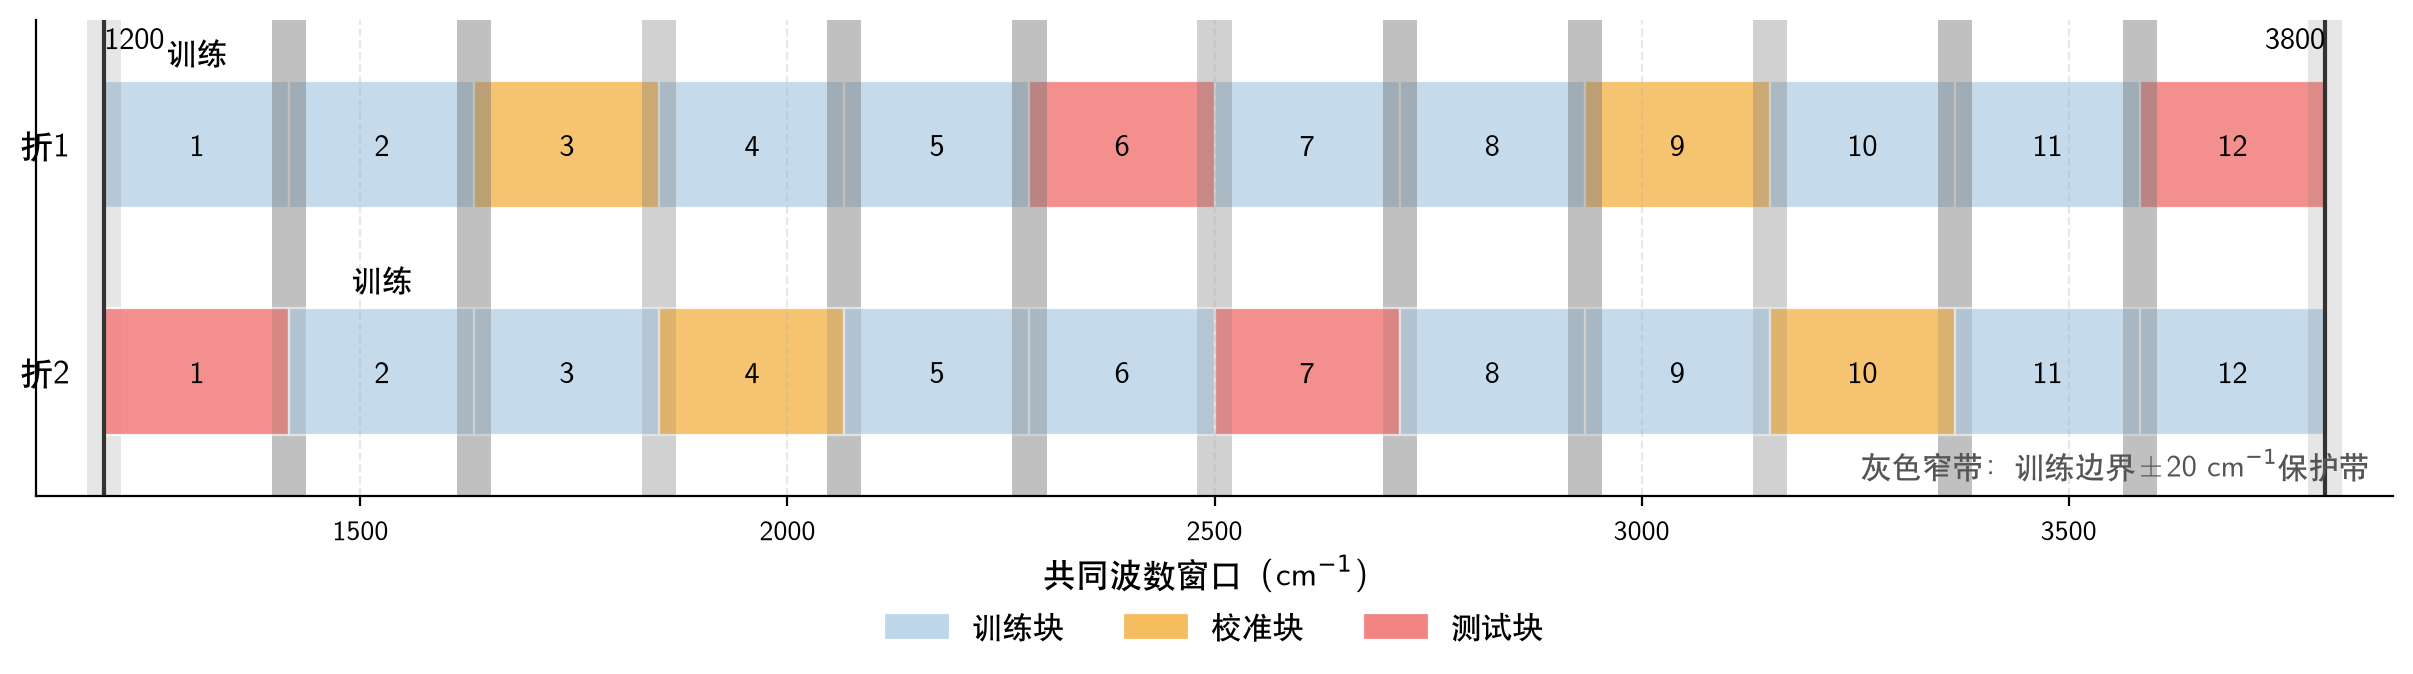
\includegraphics[width=0.8\textwidth,height=35.7mm,keepaspectratio]{../求解/问题2/图片/连续留段隔离拟合与检验.png}
  \caption{两角同步留段的训练校准测试区段}
  \label{fig:split}
\end{figure}

末端$3800$--$4000.122\ \mathrm{cm}^{-1}$另作外层检验，保护窗口为$3750$--$3800\ \mathrm{cm}^{-1}$。
% src:求解/问题2/结果/基准交接.json:末端新留段.0.测试窗口_cm^-1;末端新留段.0.保护窗口_cm^-1

两谱的原始相关系数为$0.9987$，但反射率均方根差仍有$2.14$个百分点。初次以双角高相关评价厚度可靠性，核对后改为同波数双角分组，以训练尺度归一化的留段预测误差比较方法。波数逐行对齐决定双角同步分组，同片物理条件决定共享厚度；原谱高相关包含慢变基线，留段预测用于检验模型对谱形的解释。
% src:交接/数据档案.json:跨文件关系.两两全量核验.0.原始反射率皮尔逊相关系数;跨文件关系.两两全量核验.0.均方根差;跨文件关系.同片分组
% src:交接/实验记录.json:50.尝试;50.现象;50.决定

超界观测来自附件2，共有$262$个反射率超过$100\%$的原值，所在区间与主拟合窗口不相交，点数及波数范围列入表\ref{tab:05}。这些观测不参与主拟合窗口拟合，原文件保持不变。
% src:交接/数据档案.json:文件档案.1.工作表.0.反射率检查.超过百分之百点数;文件档案.1.工作表.0.反射率检查.超过百分之百区段.0.起始波数;文件档案.1.工作表.0.反射率检查.超过百分之百区段.0.终止波数
% src:求解/问题2/结果/数据审查.json:主窗口_cm^-1;质量处置

附件一（十度入射）在$500$--$1000$与$3000$--$3500\ \mathrm{cm}^{-1}$两段的反射率散布明显不同，表\ref{tab:05}保留其标准差。这里的标准差衡量一段光谱内反射率围绕平均值的起伏大小，既包含慢变包络，也包含条纹变化。
% src:交接/数据档案.json:文件档案.0.入射角度;文件档案.0.工作表.0.分波段描述.1.左闭右开波数区间;文件档案.0.工作表.0.分波段描述.6.左闭右开波数区间;文件档案.0.工作表.0.分波段描述.1.反射率统计.样本标准差;文件档案.0.工作表.0.分波段描述.6.反射率统计.样本标准差

选型时曾核对绝对振幅反演与峰谷序列反演对包络和校准的依赖，分段散布差异促使慢变部分与条纹分别处理。包络和条纹幅值随波段变化，因此用逐角低阶响应描述慢变部分，即各角度的基线最高取二次、幅值最高取一次；两角损失以训练残差尺度归一化，该尺度描述训练段扣除二次基线后剩余差异的散布，原谱标准差则描述总体起伏。峰序与相位回归承担独立核对，同片厚度由双角共享参数的主方法给出。
% src:交接/实验记录.json:39.尝试;39.现象;39.决定
% 依据:交接/建模笔记_问题2.md:4.投影求解与厚度搜索

“双角色散变投影”就是先给定厚度和折射变化，再从观测中求出各角度的基线与振幅，让搜索集中在较少的物理参数上。两种角度共同决定厚度$d$、参考折射率参数$n_0$与色散参数$c$，每个角度自己解释慢变基线、振幅和常相位偏置$\psi_\theta$。给定这些非线性参数后，再用线性投影求各角度的二次基线系数$b_{\theta,0},b_{\theta,1},b_{\theta,2}$和一次幅值系数$a_{\theta,0},a_{\theta,1}$；因此干扰项有边界，不能扩张为逐波数自由相位。逐角独立求厚后再平均也被排除，因为它既丢掉同片约束，也无法说明两角差异来自何处。表\ref{tab:05}将窗口、区段职责和参数角色集中列出；其中触边解指参数达到预设取值上下限的候选解。

\begingroup
\scriptsize
\setlength{\tabcolsep}{2pt}
\begin{longtable}{>{\centering\arraybackslash}p{0.12\textwidth} >{\centering\arraybackslash}p{0.28\textwidth} >{\centering\arraybackslash}p{0.26\textwidth} >{\centering\arraybackslash}p{0.22\textwidth}}
\caption{问题二数据切分与参数搜索口径}\label{tab:05}\\
\hline
环节 & 主设置 & 参数角色 & 作用\\
\hline
主拟合窗口 & $1200$--$3800\ \mathrm{cm}^{-1}$ & $480$点、$12$个连续块 & 双角同步取样\\
第一折 & 训练：$1,2,4,5,7,8,10,11$ & 校准：$3,9$ & 测试：$6,12$\\
第二折 & 训练：$2,3,5,6,8,9,11,12$ & 校准：$4,10$ & 测试：$1,7$\\
区段隔离 & 训练边界保护带$20\ \mathrm{cm}^{-1}$ & 测试块只计分 & 减轻邻近信息串入\\
超百分百点 & $801.278$--$927.1104\ \mathrm{cm}^{-1}$ & 附件2，$262$点 & 原值保留，主窗外\\
低波数段 & $500$--$1000\ \mathrm{cm}^{-1}$ & 标准差$28.9$个百分点 & 附件一，十度入射\\
高波数段 & $3000$--$3500\ \mathrm{cm}^{-1}$ & 标准差$0.189$个百分点 & 附件一，十度入射\\
变投影 & 共享$d,n_0,c$；分角常相位$\psi_\theta$ & 给定非线性量后解线性系数 & 保留共同条纹与角度差异\\
搜索边界 & $d\in[0.5,40]\ \mu\mathrm{m}$ & $n_0\in[1.2,6]$；$c\in[-1,1]$ & 每个情景重新估计\\
粗网格 & 厚度$96$点网格$\times9$个光学情景 & 局部起点最多$12$个 & 多起点局部细化\\
停止条件 & 单情景预算$42\ \mathrm{s}$；固定参数须一致 & 只保留满足物理约束的候选 & 避免以触边解缩窄范围\\
\hline
\end{longtable}
\endgroup
% src:求解/问题2/结果/数据审查.json:主窗口_cm^-1;抽样点数_每角度;抽样索引
% src:求解/问题2/结果/基准交接.json:训练保护带_cm^-1;折分.0.训练块;折分.0.校准块;折分.0.测试块;折分.1.训练块;折分.1.校准块;折分.1.测试块
% src:交接/数据档案.json:文件档案.1.工作表.0.反射率检查.超过百分之百点数;文件档案.1.工作表.0.反射率检查.超过百分之百区段.0.起始波数;文件档案.1.工作表.0.反射率检查.超过百分之百区段.0.终止波数;文件档案.0.工作表.0.分波段描述.1.左闭右开波数区间;文件档案.0.工作表.0.分波段描述.6.左闭右开波数区间;文件档案.0.工作表.0.分波段描述.1.反射率统计.样本标准差;文件档案.0.工作表.0.分波段描述.6.反射率统计.样本标准差;文件档案.0.入射角度
% 依据:交接/建模笔记_问题2.md:4.2 搜索、全量答案与剖面;2.2 经验色散而非记忆常数
% src:求解/问题2/结果/验证.json:搜索.0.搜索预算秒;搜索.1.搜索预算秒;搜索.0.粗网格计划次数;搜索.1.粗网格计划次数

在共享物理参数与分角线性响应的分工下，下一节给出消去线性系数后的联合目标。

\subsubsection{模型建立：共同厚度的色散变投影}

同片双角共享厚度和折射变化，基线、幅值与固定相位则分别估计。先前考虑逐角求厚再平均，却会丢失同片约束，因而改用这项分工。
% src:交接/实验记录.json:34.尝试;34.现象;34.决定

令$d$为厚度（$\mu\mathrm{m}$），$\sigma$为波数（$\mathrm{cm}^{-1}$），$\theta\in\{10^\circ,15^\circ\}$为入射角。透明各向同性假设下，实折射率$n(\sigma)$与一次往返相位$\Phi_\theta$满足
\begin{equation}
n(\sigma)=n_0+c\left[\left(\frac{\sigma_0}{\sigma}\right)^2-1\right],\qquad
\Phi_\theta=4\pi\,10^{-4}d\sigma\sqrt{n(\sigma)^2-\sin^2\theta}.
\label{eq:q2-phase}
\end{equation}
其中$n_0$为参照波数$\sigma_0=2000\ \mathrm{cm}^{-1}$处的折射率，$c$为无量纲色散参数，$10^{-4}$将微米换为厘米；传播要求$n(\sigma)>\sin15^\circ$。缺少实测折射率，故用这两个参数描述折射变化。
% src:交接/数据档案.json:总览.每块晶圆入射角度;未随附件提供的建模输入
% src:交接/计划.json:问题清单.1.建模步骤.2
% src:求解/问题2/结果/厚度结果.json:光学情景.传播约束

取训练波数的中点$\bar\sigma$与半跨度$h$，令$x=(\sigma-\bar\sigma)/h$，以比例反射率$y_\theta$写出观测式
\begin{equation}
y_\theta=b_{\theta,0}+b_{\theta,1}x+b_{\theta,2}x^2
+ (a_{\theta,0}+a_{\theta,1}x)\cos(\Phi_\theta+\psi_\theta)+\varepsilon_\theta.
\label{eq:q2-model}
\end{equation}
系数$b_{\theta,j}$和$a_{\theta,j}$分别描述基线与幅值，$\psi_\theta$为常相位，$\varepsilon_\theta$为残差。前节两角反射率并不相同，因此用各角低阶响应吸收慢变背景和包络差异；二次基线、一次幅值是限制干扰自由度的工作假设，其影响由改变阶数后的重新估计检查。幅值可变号而相位固定，避免自由相位吞掉条纹。
% src:求解/问题2/结果/厚度结果.json:全量拟合参数.基线阶数;全量拟合参数.幅值阶数;灵敏度情景搜索完整性

给定共享参数$\eta=(d,n_0,c)$和$\psi_\theta$，令$z_\theta=\cos(\Phi_\theta+\psi_\theta)$。变投影先解角度响应，再搜索物理参数，线性部分只含五列（表\ref{tab:05}）：
\begin{equation}
X_\theta=[1,x,x^2,z_\theta,xz_\theta],\qquad
\widehat{\boldsymbol\beta}_\theta=\mathop{\arg\min}_{\boldsymbol\beta_\theta}
\|\boldsymbol y_\theta-X_\theta\boldsymbol\beta_\theta\|_2^2.
\label{eq:q2-projection}
\end{equation}
其中$X_\theta$在训练点逐行取值，$\boldsymbol y_\theta$为观测向量，系数向量$\boldsymbol\beta_\theta$按$X_\theta$列序排列。外层在表\ref{tab:05}约束内最小化两角等权损失
\begin{equation}
L(\eta)=\frac12\sum_{\theta\in\{10^\circ,15^\circ\}}
\min_{0\leq\psi_\theta<\pi}
\frac{\|\boldsymbol y_\theta-X_\theta\widehat{\boldsymbol\beta}_\theta\|_2^2}{N_\theta s_\theta^2}.
\label{eq:q2-loss}
\end{equation}
训练点数记为$N_\theta$，$s_\theta$取训练二次趋势残差的四分位距，下限为$10^{-4}$，搜索中固定。用去趋势后的尺度归一化，使两角的幅值差异不直接决定损失权重；该尺度只在训练点计算并在搜索中固定。幅值变号可吸收$\pi$的相位平移，故常相位只搜索半周期。

粗网格搜索以$96$个厚度点覆盖$0.5$--$40\ \mu\mathrm{m}$，再从多起点有界细化并全量重拟合。
% src:交接/计划.json:问题清单.1.验证方案.灵敏度.3
% src:求解/问题2/结果/基准交接.json:灵敏度情景.0.厚度网格点数

参数搜索范围就是计算时允许各参数变化的上下限，并非材料测量给出的取值范围。参考折射率允许$n_0\in[1.2,6]$，色散参数允许$c\in[-1,1]$，并须满足前述传播约束；这些边界会排除范围外的组合，多起点用于比较范围内不同厚度与折射率组合。
% src:交接/计划.json:问题清单.1.验证方案.灵敏度.3

相位中厚度与折射因子相乘，折射率下降可由厚度增大补偿。

全量拟合厚度为$10.80\ \mu\mathrm{m}$，参考折射率为$1.4930$。相位中的厚度与折射因子相乘，不同组合可以产生相近条纹，因而继续检查损失接近最小值的候选解。
% src:求解/问题2/结果/厚度结果.json:同片最佳厚度_微米;同片最佳厚度的参考折射率

连续切分、光学参数补偿以及基线和色散形式改变，共同形成$0.64$--$18.11\ \mu\mathrm{m}$的厚度重估范围（图\ref{fig:q2-thickness}）。令$D$为纳入范围的候选厚度集合，$I_{\mathrm{cond}}$为其最外端点构成的区间，则
% src:求解/问题2/结果/厚度结果.json:条件区间_微米;条件区间组成
\begin{equation}
\begin{aligned}
D&=D_2\cup D_5\cup D_{\mathrm{prof}}\cup D_{\mathrm{sens}},\\
I_{\mathrm{cond}}&=[\min D,\max D].
\end{aligned}
\label{eq:q2-range}
\end{equation}
其中$D_2$、$D_5$分别收集两折、五折连续留段重新拟合的候选厚度；$D_{\mathrm{prof}}$固定全量拟合色散，逐点重估厚度与参考折射率网格上的各角响应，收集损失不超过剖面最小值$1.10$倍的厚度，称为近等损失剖面候选。
% src:求解/问题2/结果/厚度结果.json:条件区间构造;条件区间组成.两折条件厚度_微米;条件区间组成.五折条件厚度_微米;条件区间组成.光学剖面厚度范围_微米

$D_{\mathrm{sens}}$收集改变基线、幅值、色散或波段后重新估计的厚度，按“是否纳入厚度重估范围”筛选；满足传播约束和指定参数条件且被列为纳入的候选进入集合，人为改动指定参数的边界调整结果排除在外。这些候选对应各自的模型设置与参数约束，$I_{\mathrm{cond}}$汇集它们的最外端点，记录厚度随估计条件的变化。
% src:求解/问题2/结果/厚度结果.json:条件区间构造;条件区间组成.灵敏度情景厚度_微米;灵敏度情景搜索完整性

下一节据共同相位与逐角响应，报告两角预测、留段误差及反射率覆盖的缺口。

\subsubsection{求解与结果分析：碳化硅厚度及双角核对}

共享厚度与逐角低阶响应分开后，求解的重点便是交出厚度，并检查这个数能否解释未参与拟合的光谱。这里先报告同片结果，再用连续留段和双向留角度核对条纹。

碳化硅外延层的同片非触边代表厚度为$10.80\ \mu\mathrm{m}$，厚度重估范围为$0.64$--$18.11\ \mu\mathrm{m}$。点值对应透明两束、经验色散及逐角低阶响应；范围则记录搜索、切分和光学条件变化带来的厚度移动。表\ref{tab:q2-results}将计算设置、同片代表值与分项核对并列，两个附件共同决定厚度，而非分别求厚后取平均。
% src:求解/问题2/结果/厚度结果.json:同片最佳厚度_微米;条件区间_微米;光学情景;输入附件

这里采用的是固定比较基准的规则，而非加密后重新选优：在原厚度网格$96$点搜索内取最低损失可行解，各参数距上下界的距离除以搜索跨度后均须大于$10^{-4}$。原点的最小相对边界距离为$0.0610$，满足该规则；表\ref{tab:q2-search-check}中的加密触边候选仍参与全部候选的损失比较，不因触边而被排除。
% src:求解/问题2/结果/搜索补查.json:代表点规则;候选.0.最小相对边界距离

按训练损失排序，现有补查最低的厚度是$13.53\ \mu\mathrm{m}$，不是沿用的$10.80\ \mu\mathrm{m}$。前者折射率触及搜索下界，后者承担跨问题比较坐标；这两个身份分列，搜索产生的分支差异也与改变光学假设的情景差异分别讨论。厚度保留两位小数是报告格式，测量精度仍受光学假设和取段变化限制。
% src:求解/问题2/结果/搜索补查.json:候选.0.厚度_微米;补查最低损失候选.厚度_微米;补查最低损失候选.触边参数

附件一（十度）与附件二（十五度）在共同原始坐标上同步抽样。给定厚度与折射变化后，先直接求出各角基线和幅值，再作多起点有界搜索；这种安排把条纹位置留给共享参数，把角度造成的包络差别交给低阶响应。连续块承担训练、校准和测试的不同任务，训练边界另留$20\ \mathrm{cm}^{-1}$保护带，避免相邻波数点混入留段检验。
% src:求解/问题2/结果/基准交接.json:训练保护带_cm^-1
% src:求解/问题2/结果/数据审查.json:文件.0.入射角度_度;文件.1.入射角度_度

% 表06
\begingroup
\small
\begin{longtable}{>{\centering\arraybackslash}p{0.20\textwidth}>{\centering\arraybackslash}p{0.24\textwidth}>{\centering\arraybackslash}p{0.20\textwidth}>{\centering\arraybackslash}p{0.24\textwidth}}
\caption{碳化硅计算条件与厚度核对}\label{tab:q2-results}\\
\toprule
项目 & 设置或结果 & 项目 & 设置或结果\\
\midrule
\endfirsthead
\toprule
项目 & 设置或结果 & 项目 & 设置或结果\\
\midrule
\endhead
主拟合窗口 & $1200$--$3800\ \mathrm{cm}^{-1}$ & 原坐标采样 & 每角$480$点\\
逐角基线 & 二次 & 逐角幅值 & 一次\\
参考折射率 & $1.4930$ & 色散系数 & $-0.2089$\\
全量同片厚度 & $10.80\ \mu\mathrm{m}$ & 厚度重估范围 & $0.64$--$18.11\ \mu\mathrm{m}$\\
五折厚度范围 & $5.53$--$13.51\ \mu\mathrm{m}$ & 五折相对极差 & $0.7604$\\
正式留段误差 & $1.2074$ & 二次趋势误差 & $1.4404$\\
谱形相对改善 & $16.17\%$ & 测试经验覆盖 & $49.06\%$\\
原型主方法误差 & $1.1717$ & 原型峰序误差 & $1.2354$\\
原型相位误差 & $1.2202$ & 误差及极差单位 & 无量纲\\
\midrule
测试区段 & $10^\circ\!\to15^\circ$误差 & 测试区段 & $15^\circ\!\to10^\circ$误差\\
首折第六块 & $0.501$ & 首折第六块 & $0.257$\\
首折第十二块 & $1.186$ & 首折第十二块 & $1.087$\\
次折第一块 & $3.457$ & 次折第一块 & $2.965$\\
次折第七块 & $0.168$ & 次折第七块 & $0.249$\\
\bottomrule
\end{longtable}
\endgroup
% src:求解/问题2/结果/数据审查.json:主窗口_cm^-1;抽样点数_每角度;文件.0.入射角度_度;文件.1.入射角度_度
% src:求解/问题2/结果/厚度结果.json:同片最佳厚度_微米;同片最佳厚度的参考折射率;同片最佳厚度的经验色散系数;条件区间_微米
% src:求解/问题2/结果/验证.json:搜索.0.基线阶数;搜索.0.幅值阶数;五折跨切分稳定性.最小厚度_微米;五折跨切分稳定性.最大厚度_微米;五折跨切分稳定性.相对极差;正式主方法分数_连续留段标准化均方根误差;正式二次趋势基线分数_连续留段标准化均方根误差;正式主方法相对正式二次趋势改善_百分比;三路线原型对比.双角色散变投影;三路线原型对比.双角峰序匹配;三路线原型对比.双角相位回归;双向留角度冻结诊断
% src:求解/问题2/结果/区间覆盖.json:测试经验覆盖率

宽范围来自厚度与折射率的互相补偿：不同组合可以解释相近的条纹。五折厚度的相对极差为$0.7604$，即最大与最小厚度之差除以中位数；图\ref{fig:q2-thickness}把这种切分移动与光学情景分开。范围按式\eqref{eq:q2-range}取两折、五折、光学剖面及满足参数约束的灵敏度候选的最外端点，其中剖面保留训练损失较最小值增加不超过$10\%$的组合。
% src:求解/问题2/结果/验证.json:五折跨切分稳定性.相对极差
% src:求解/问题2/结果/厚度结果.json:条件区间构造;条件区间组成

% 图13
\begin{figure}[H]
  \centering
  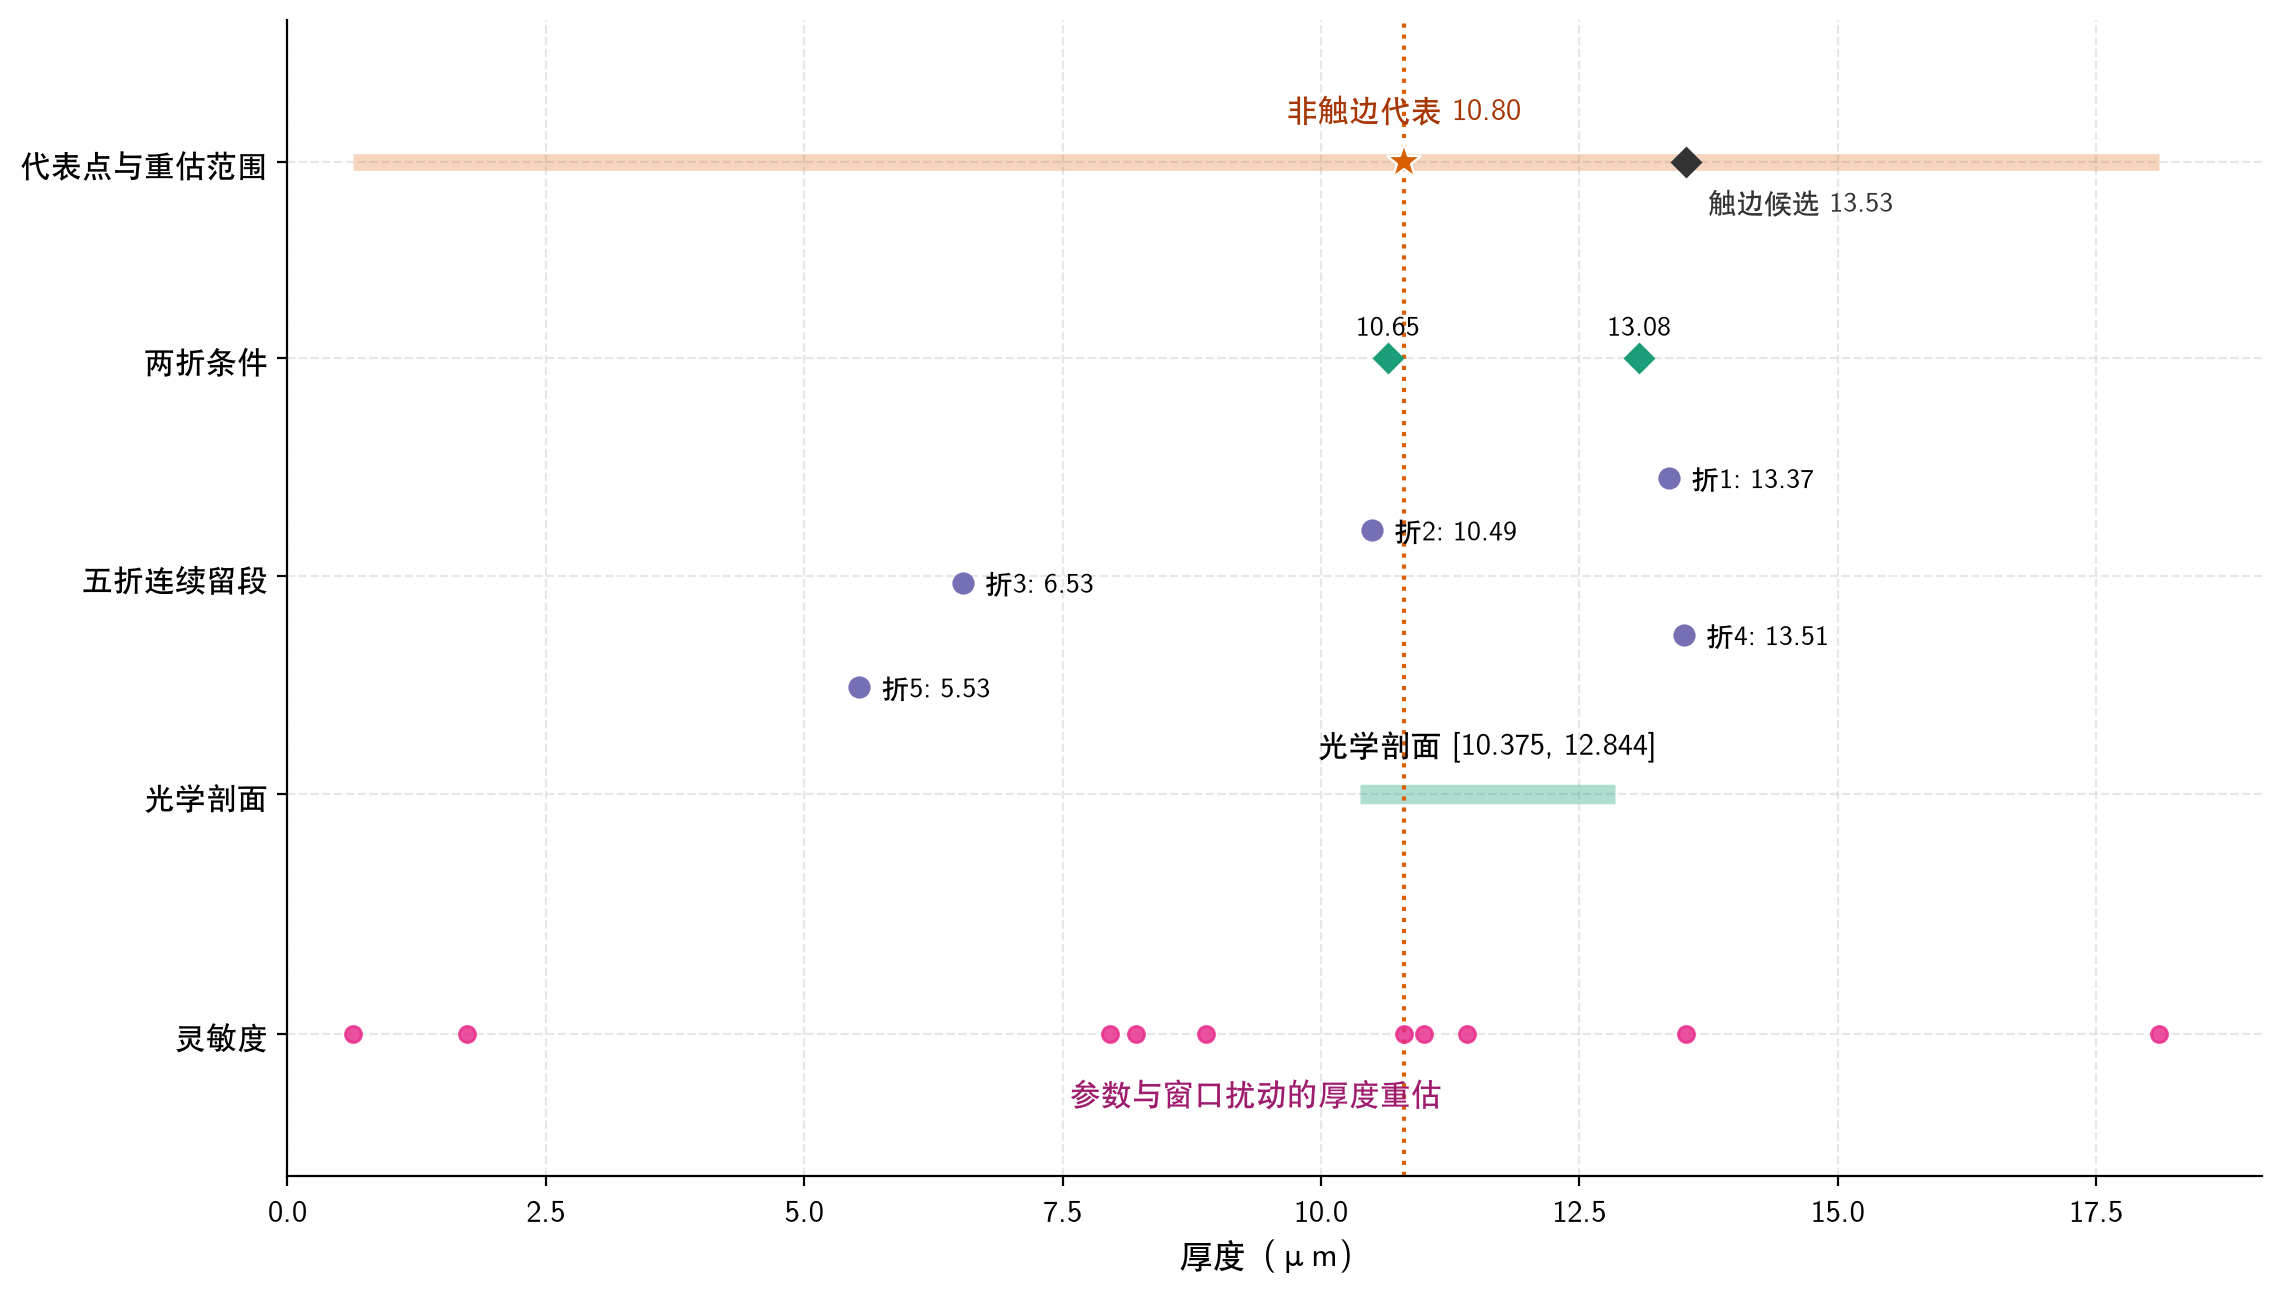
\includegraphics[width=0.8\textwidth,height=72.5mm,keepaspectratio]{../求解/问题2/图片/碳化硅厚度随假设变化.png}
  \caption{碳化硅厚度随切分和光学设置变化}
  \label{fig:q2-thickness}
\end{figure}

厚度分支虽随区段移动，条纹项仍增加了对留出光谱的解释力。正式连续留段标准化均方根误差为$1.2074$，低于二次趋势基线的$1.4404$，相对改善$16.17\%$；两项误差均无量纲，表示反射率预测误差相对于训练残差尺度的大小，按测试块等权平均。图\ref{fig:q2-residual}并列整体预测与局部残差，展示条纹拟合的总体优势和仍有偏差的波数区段。
% src:求解/问题2/结果/验证.json:正式主方法分数_连续留段标准化均方根误差;正式二次趋势基线分数_连续留段标准化均方根误差;正式主方法相对正式二次趋势改善_百分比;主指标含义

% 图10
\begin{figure}[!htb]
  \centering
  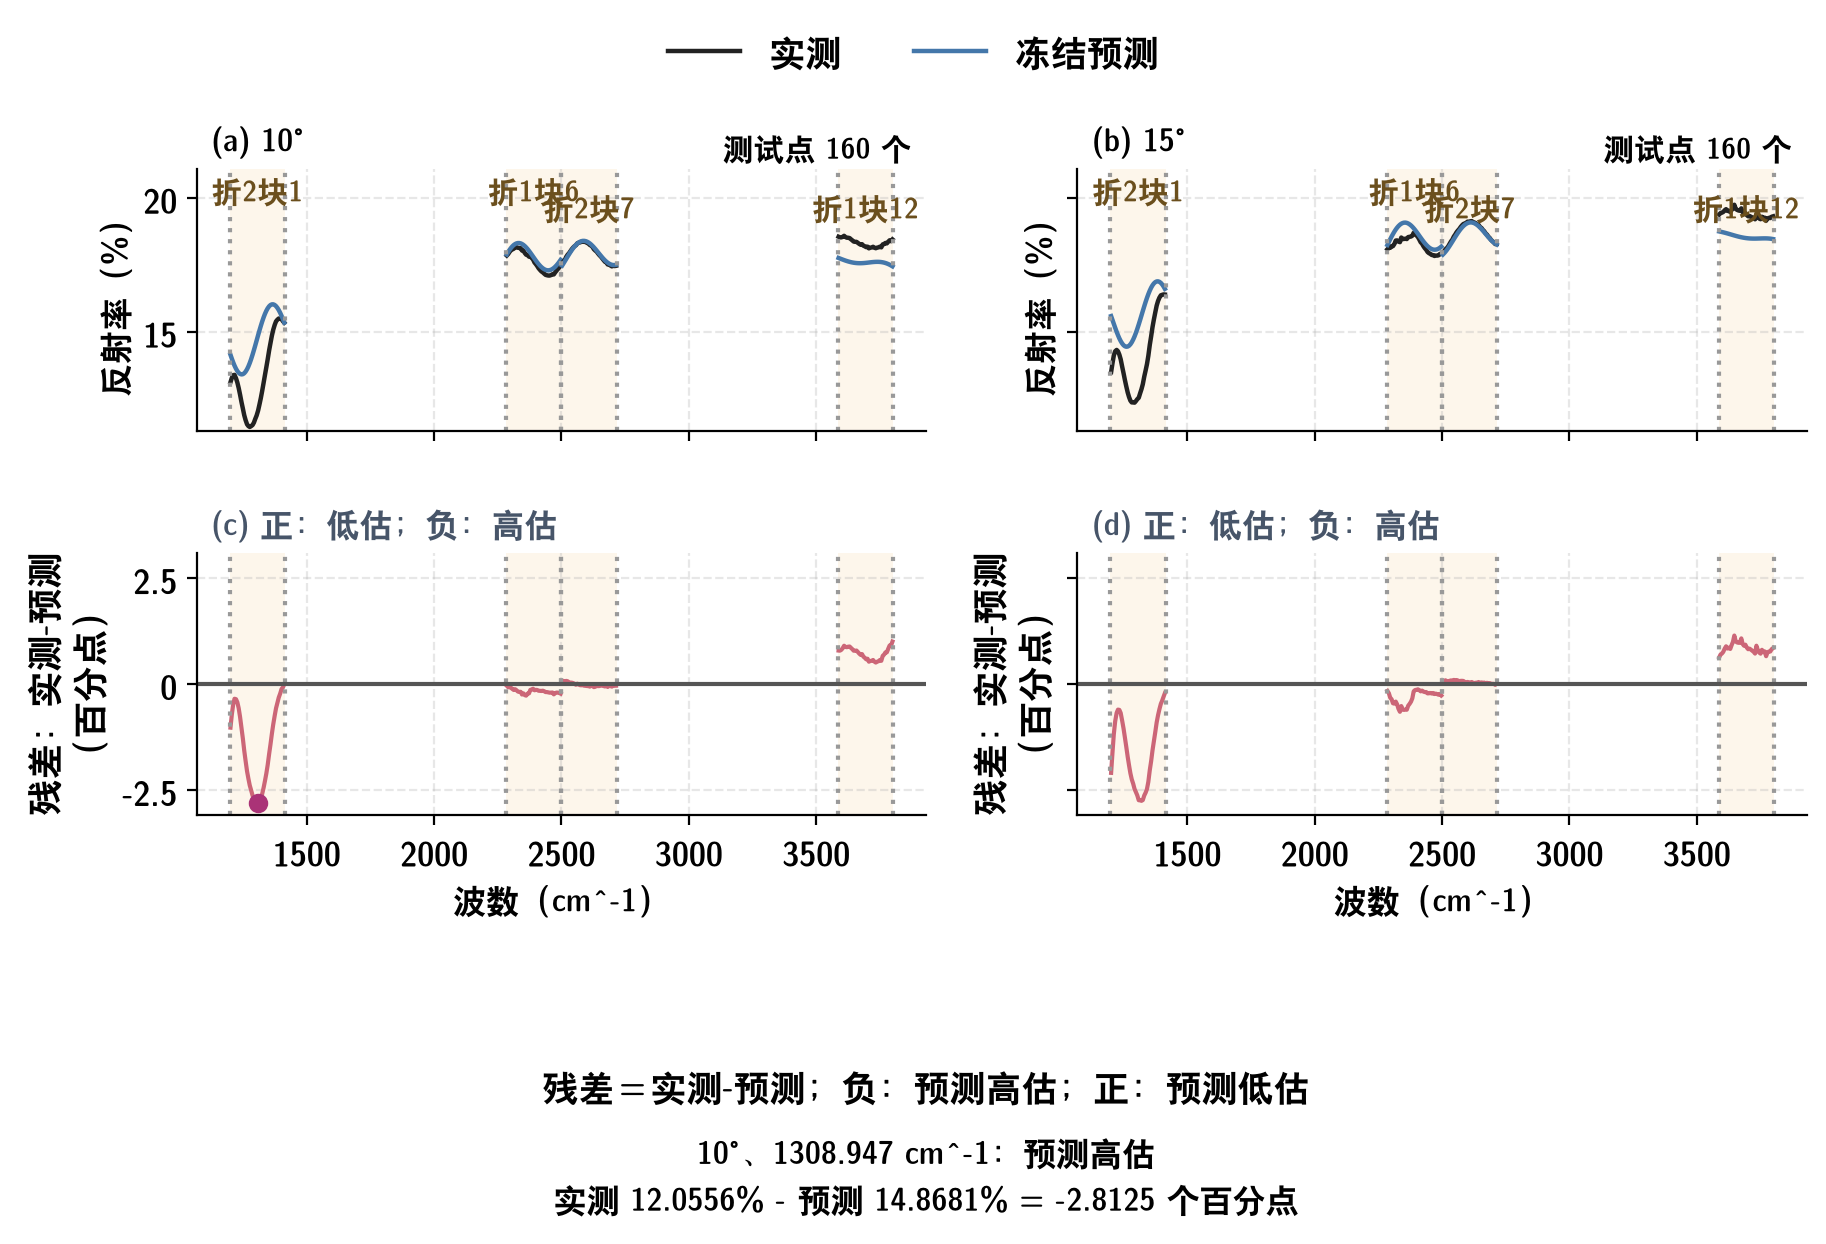
\includegraphics[width=0.96\textwidth]{../求解/问题2/图片/双角拟合残差显示局部偏差.png}
  \caption{双角光谱预测显示局部残差}
  \label{fig:q2-residual}
\end{figure}

局部偏差也曾改变区间的解释。最初把经验区间称为名义$90\%$区间时，连续测试块覆盖率仅为$50.63\%$；这次核对促使区间改用固定经验分位描述，并单独报告留出观测实际落入区间的比例。
% src:交接/实验记录.json:506.尝试;506.现象;506.决定

当前反射率区间以校准块绝对残差的$75\%$经验分位作为对称半宽，即将校准偏差由小到大排列，取该位置的偏差加在预测值两侧；测试经验覆盖率为$49.06\%$。图\ref{fig:q2-coverage}以校准分位为参照线，分块偏离说明校准段的误差宽度没有充分容纳测试段的偏差。
% src:求解/问题2/结果/区间覆盖.json:构造方法;校准经验分位点;测试经验覆盖率;覆盖解释

% 图14
\begin{figure}[!htb]
  \centering
  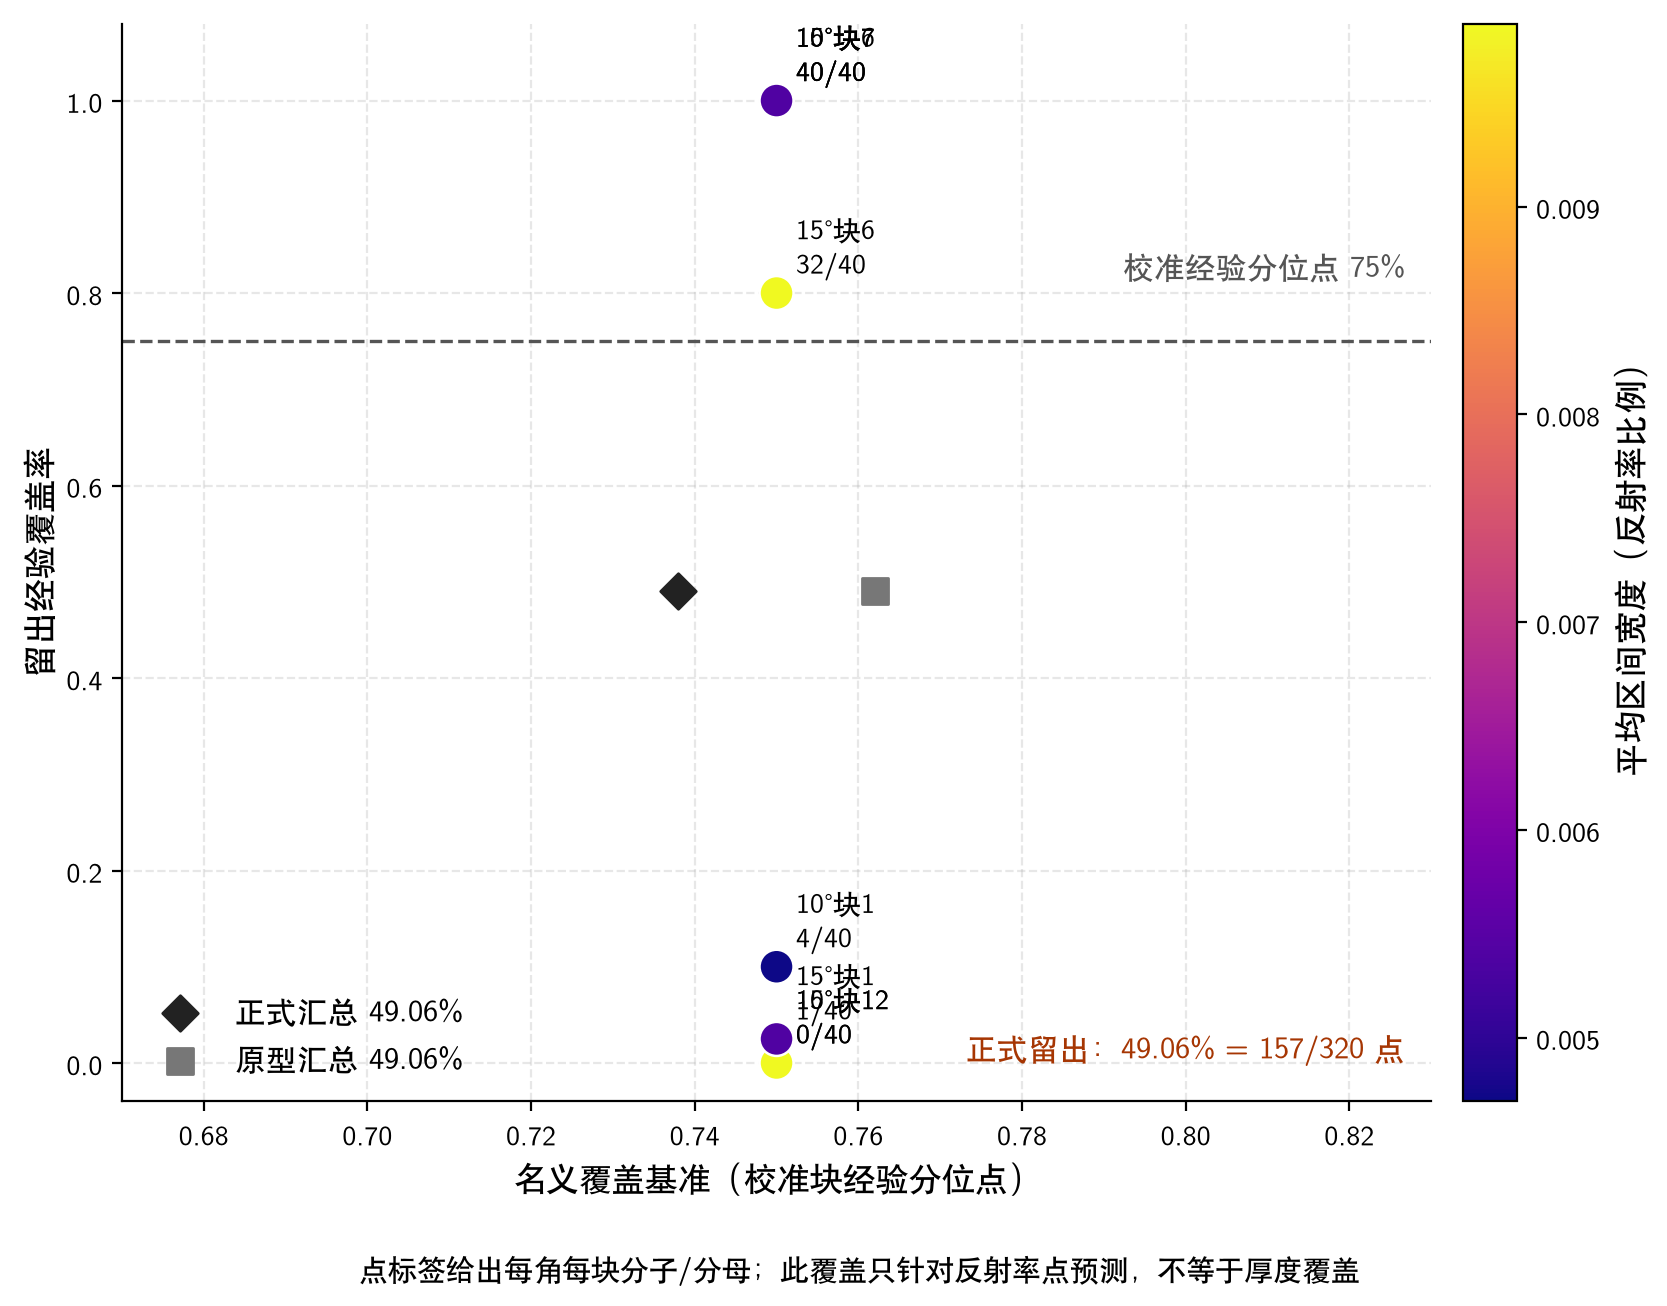
\includegraphics[width=0.8\textwidth,height=100mm,keepaspectratio]{../求解/问题2/图片/预测覆盖揭示区间失配.png}
  \caption{留出反射率覆盖偏离校准分位水平}
  \label{fig:q2-coverage}
\end{figure}

覆盖缺口把注意力引向跨角度的局部偏差。双向留角度核对固定每折共享厚度、色散及来源角相位，只在目标角训练点重估低阶基线与幅值；另一角的偏差便无法再靠自由调整厚度吸收。误差最大的测试块在正、反方向分别达到$3.457$和$2.965$，均无量纲，图\ref{fig:q2-angle}与表\ref{tab:q2-results}保留了其余块的差别。
% src:求解/问题2/结果/验证.json:双向留角度冻结诊断.4;双向留角度冻结诊断.6

% 图12


双向核对检验同片参数跨角度解释谱形的能力，碳化硅的同片拟合厚度为$10.80\ \mu\mathrm{m}$，厚度重估范围为$0.64$--$18.11\ \mu\mathrm{m}$。本问置信等级为低：五折厚度随切分明显变化，反射率测试覆盖不足，灵敏度情景形成较宽的厚度重估范围。该范围汇集光学假设下的重估结果，不是概率区间，反射率覆盖率也不是厚度覆盖率，绝对厚度仍需光学标定或标准厚度样片核对。问题三据此保留两束模型基准，检验更高阶往返是否足以改变这块晶圆的厚度判断。
% src:求解/问题2/结果/厚度结果.json:同片最佳厚度_微米;条件区间_微米
% src:交接/结果声明_问题2.json:置信.等级;置信.理由

\subsection{问题三的建模与求解：逐次往返厚度对照}

上一问给出了碳化硅的两束模型基准，本问采用逐次往返厚度对照，在相同设置下比较两束截断场与完整往返场。完整往返场将表面反射与各轮返回相加，往返衰减场反演据此计算反射率，再搜索与观测相符的厚度。硅在这一框架下求厚度，碳化硅则在高阶往返可观测且影响厚度时修正。

完整往返场给出硅全量厚度 $2.17\ \mu\mathrm{m}$，两次连续留段分别为 $1.73$、$16.04\ \mu\mathrm{m}$；碳化硅缺少相干、空间重叠和仪器分辨率资料，保留前问基准 $10.80\ \mu\mathrm{m}$。
% src:求解/问题3/结果/回炉轮3候选/仲裁闭环/20260910_131501_81623_建模公式/厚度结果.json:核心指标.硅全量完整往返厚度_um;核心指标.硅折1完整往返条件厚度_um;核心指标.硅折2完整往返条件厚度_um;核心指标.碳化硅正式基准厚度_um

两材料在同波段、同留出点及同响应设置下比较，完整往返场的总体标准化留段均方根误差为 $1.0231$，高于两束的 $0.9812$（均无量纲）。逐块收益随材料和区段改变，完整场并未取得总体预测优势。这个分歧要求先核对观测条件与资料缺口，再推导往返场及其厚度影响。
% src:求解/问题3/结果/回炉轮3候选/仲裁闭环/20260910_131501_81623_建模公式/厚度结果.json:分材料验证.硅.逐折汇总.0.平均标准化均方根误差.两束;分材料验证.硅.逐折汇总.0.平均标准化均方根误差.完整往返;分材料验证.硅.逐折汇总.0.平均标准化均方根误差.训练均值;分材料验证.硅.逐折汇总.0.平均标准化均方根误差.二次趋势;分材料验证.硅.逐折汇总.1.平均标准化均方根误差.两束;分材料验证.硅.逐折汇总.1.平均标准化均方根误差.完整往返;分材料验证.硅.逐折汇总.1.平均标准化均方根误差.训练均值;分材料验证.硅.逐折汇总.1.平均标准化均方根误差.二次趋势;分材料验证.碳化硅.逐折汇总.0.平均标准化均方根误差.两束;分材料验证.碳化硅.逐折汇总.0.平均标准化均方根误差.完整往返;分材料验证.碳化硅.逐折汇总.0.平均标准化均方根误差.训练均值;分材料验证.碳化硅.逐折汇总.0.平均标准化均方根误差.二次趋势;分材料验证.碳化硅.逐折汇总.1.平均标准化均方根误差.两束;分材料验证.碳化硅.逐折汇总.1.平均标准化均方根误差.完整往返;分材料验证.碳化硅.逐折汇总.1.平均标准化均方根误差.训练均值;分材料验证.碳化硅.逐折汇总.1.平均标准化均方根误差.二次趋势
% src:交接/实验记录.json:563.尝试;563.现象;563.决定

\subsubsection{分析与准备：必要条件对应观测证据}

多光束判定须分清形成、计算、观测与测厚影响。非零界面返回、时间相干、空间重叠与仪器分辨四类条件缺一不可；两个界面存在只涉及首项。

往返复倍率即每轮返回场的共同衰减与相位因子。其最大模（幅度比例）在硅两次留段为$0.1333$和$0.0769$，碳化硅为$0.0258$和$0.0076$，均无量纲；图\ref{fig:roundtrip}中的光路说明相邻返回为何乘以同一复数，收敛与实验观测由不同条件控制。
% src:求解/问题3/结果/公平对照.json:案例.1.场级数核验.最大往返乘子模;案例.2.场级数核验.最大往返乘子模;案例.4.场级数核验.最大往返乘子模;案例.5.场级数核验.最大往返乘子模

\begingroup
\setlength{\intextsep}{2pt}
\begin{figure}[H]
  \centering
  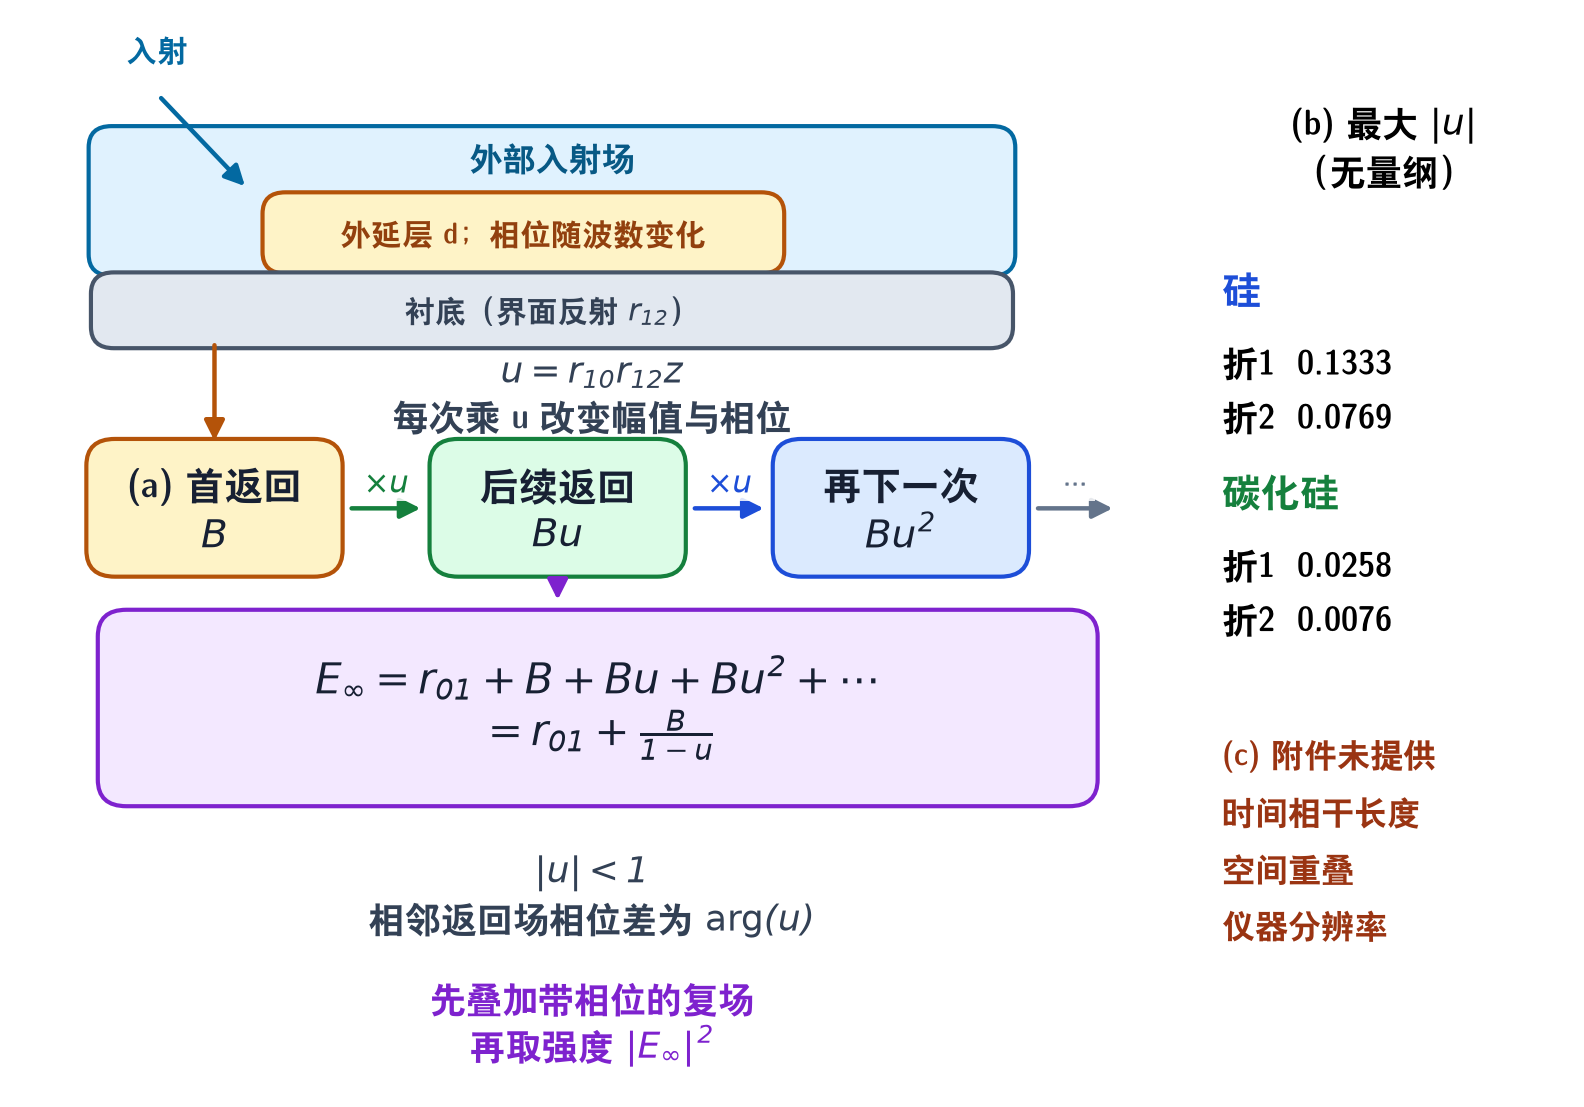
\includegraphics[width=0.96\textwidth]{../求解/问题3/图片/多次往返按复振幅递减.png}
  \caption{返回光的复振幅随往返次数递减}
  \label{fig:roundtrip}
\end{figure}
\endgroup

逐项核对发现，硅双角原始相关系数虽达$0.9943$，相干、重叠及分辨资料却均缺失，因而排除高相关直接判定；表\ref{tab:07}把已知量与未知量分列。
% src:交接/数据档案.json:跨文件关系.两两全量核验.5.原始反射率皮尔逊相关系数
% src:交接/实验记录.json:547.尝试;547.现象;547.决定

\begingroup
\footnotesize
\setlength{\LTpre}{3pt}
\setlength{\LTpost}{3pt}
\begin{longtable}{>{\centering\arraybackslash}p{0.16\textwidth} >{\centering\arraybackslash}p{0.18\textwidth} >{\centering\arraybackslash}p{0.17\textwidth} >{\centering\arraybackslash}p{0.16\textwidth} >{\centering\arraybackslash}p{0.17\textwidth}}
\caption{多光束必要条件与四附件证据}\label{tab:07}\\
\hline
必要条件 & 核对对象 & 四附件已有信息 & 缺失信息 & 替代解释\\
\hline
界面返回 & 界面反射系数 & 模型可核验 & 实测光学常数 & 界面弱反射\\
时间相干 & 往返相位关联 & 均未给资料 & 相干长度 & 相位随机化\\
空间重叠 & 返回光束重合 & 均未给资料 & 光路、偏振 & 光束错位\\
仪器分辨 & 高阶谱形差 & 反射率均已给 & 分辨率、噪声 & 基线与色散\\
\hline
\end{longtable}
\endgroup
% src:求解/问题3/结果/条件判定.json:必要条件
% src:交接/数据档案.json:未随附件提供的建模输入

慢变基线也可抬高相关；折射率随波数的变化称为色散，也会改变谱形。故两束截断场与完整往返场采用同波段、同训练及留出区段、同基线复杂度，逐角评价谱形相容性。下一节沿此对照推导有限往返及收敛闭式，再讨论厚度影响。

\subsubsection{模型建立：衰减场求和与厚度偏差}

首个返回场记为$B$，后续每轮返回都乘同一往返复倍率$u$，即共同的衰减与相位因子。按几何级数求和，分清高阶返回改变的是谱形还是厚度估计。

\begingroup
\setlength{\abovedisplayskip}{4pt}
\setlength{\belowdisplayskip}{4pt}
\setlength{\abovedisplayshortskip}{2pt}
\setlength{\belowdisplayshortskip}{2pt}
\setlength{\jot}{1pt}
\setlength{\intextsep}{2pt}

沿用界面振幅系数$r_{ij},t_{ij}$，$d,\sigma,\theta$分别为厚度（$\mu\mathrm{m}$）、波数（$\mathrm{cm}^{-1}$）和入射角。令$n_1$为外延层实折射率，纵向传播因子$q_1=\sqrt{n_1^2-\sin^2\theta}$，则
\begin{equation}
\begin{aligned}
z&=\exp\!\left(-\lambda n_1/q_1+\mathrm{i}\Phi_\theta\right),\qquad
\Phi_\theta=4\pi\,10^{-4}d\sigma q_1,\\
B&=t_{01}t_{10}r_{12}z,\qquad u=r_{10}r_{12}z.
\end{aligned}
\label{eq:q3-return}
\end{equation}
其中$z,\Phi_\theta$为一次往返的传播因子与相位，$\lambda\geq0$为有效损耗；取正传播支，传播幅度不增长。保留$K$次返回的场记为$\mathcal E_K$，当$|u|<1$时
\begin{equation}
\begin{aligned}
\mathcal E_K&=r_{01}+B\sum\nolimits_{k=0}^{K-1}u^k
=r_{01}+B\frac{1-u^K}{1-u},\\
E_\infty&=r_{01}+\frac{B}{1-u},\qquad E_2=\mathcal E_1=r_{01}+B,\\
\left|E_\infty-\mathcal E_K\right|&\leq\frac{|B|\,|u|^K}{1-|u|}.
\end{aligned}
\label{eq:q3-series}
\end{equation}
这里$K$为正整数，$k$为返回阶次。尾项界给出截断误差，$u\to0$时完整往返场退回两束截断场；各次返回须先在复场上相加，再取模平方。

多光束干涉首先要求光路能产生第三束出射光。光透入外延层、在衬底反射并穿出上表面，形成$B=t_{01}r_{12}zt_{10}$；留在层内的光又经上表面内反射和衬底反射，形成$Bu=t_{01}t_{10}r_{10}r_{12}^{2}z^{2}$。因此透入、透出及两个界面的内部反射通道均须非零。级数收敛约束这些返回场的总和，探测器记录的干涉还取决于光束间的关联。记直接场振幅$a_0=r_{01}$、第$m$次返回振幅$a_m=Bu^{m-1}$，$m\geq1$。对探测区域和时间作平均，实际强度中的交叉项为
\begin{equation}
\begin{aligned}
I&=\sum_{m\geq0}|a_m|^2+
2\operatorname{Re}\sum_{m<n}a_ma_n^*\gamma_{mn}\eta_{mn},\\
J_{\mathrm{ho}}&=2\operatorname{Re}\sum_{\substack{m<n\\n\geq2}}
a_ma_n^*\gamma_{mn}\eta_{mn}.
\end{aligned}
\label{eq:q3-cross-conditions}
\end{equation}
其中$\gamma_{mn}$为两返回场的归一化时间相干度，表示相位关联经时间平均后的保留比例；$\eta_{mn}$为探测区域内的归一化空间与偏振重叠积分。$J_{\mathrm{ho}}$专指至少含一束后续返回光的干涉交叉项，不含各束自身的强度。

逐一断开光路即可检验必要性：$Bu=0$会消去全部后续返回，$\gamma_{mn}=0$会使该对光束的相位平均消失，$\eta_{mn}=0$会使探测面上的交叉积分消失。

形成高阶干涉须存在$n\geq2$的场对满足$a_ma_n^*\gamma_{mn}\eta_{mn}\ne0$，且这些交叉项合计后仍随波数变化。非零返回、相位关联与空间偏振重叠由此分别落到可检查的因子上。

相位关联和光束重叠可分别换成长度比较。令$\omega=2\pi c_0\sigma$，$c_0$为真空光速，$\phi_m$为第$m$束在同一观测面的相位，定义群时延差$\Delta\tau_{mn}=|\partial(\phi_m-\phi_n)/\partial\omega|$，等效往返光程差为$L_{mn}=c_0\Delta\tau_{mn}$。在单一相干包络、平行界面与有限宽光束的近似下，明显交叉项要求
\begin{equation}
L_{mn}\lesssim\ell_c,\qquad
|m-n|\,2d_{\mathrm{cm}}\tan\theta_1\lesssim w_b,\qquad
L_{mn}=\frac{|m-n|}{2\pi}\left|\frac{\partial\arg u}{\partial\sigma}\right|\quad(m,n\geq1).
\label{eq:q3-coherence-overlap}
\end{equation}
这里$\ell_c$为有效相干长度，$\theta_1$为层内角，$w_b$为探测面对应的光束横向尺度，所有长度统一用厘米。末式由返回场每轮累积同一相位得到，已包含传播色散和界面相位；无色散、界面相位不变时，单次光程差退化为$2d_{\mathrm{cm}}q_1$。长度比较描述常见包络下的量级要求，严格条件仍是式\eqref{eq:q3-cross-conditions}中的关联与重叠积分非零。

干涉形成后还要通过仪器响应。设$h$为归一化谱响应核，$\delta R_{\mathrm{ho}}$为$J_{\mathrm{ho}}$除以入射强度后的反射率贡献，比较时固定同一组光学参数；$\varepsilon_R$为噪声与背景分离误差尺度，则辨认高阶贡献要求
\begin{equation}
\|h*\delta R_{\mathrm{ho}}\|>\varepsilon_R,\qquad
|C_j\widehat h(f_j)|\gtrsim\varepsilon_R,\quad
f_j=\frac{j}{2\pi}\left|\frac{\partial\arg u}{\partial\sigma}\right|.
\label{eq:q3-resolution}
\end{equation}
其中$C_j$、$f_j$是相隔$j$轮的返回场交叉项在局部的振幅和波数频率，$\widehat h$是仪器响应的傅里叶变换；$\arg u$同时保留传播及界面相位。若谱响应宽度为$\delta\sigma_{\mathrm{inst}}$，避免明显平均抵消通常要求$2\pi f_j\delta\sigma_{\mathrm{inst}}\lesssim1$，严格判断仍以卷积后的幅度为准。采样间距描述相邻观测点的距离；仪器谱响应与噪声尺度则需独立标定，附件未提供这两项资料。因而$|u|<1$回答级数能否求和，非零交叉项回答干涉能否形成，响应后超出噪声才回答实验能否辨认。

曾尝试分别估计消光、界面损耗和偏振权重；因附件缺少对应标定，改用$\lambda$合并吸收与界面损失。该量描述总衰减，而非实测消光系数。
% src:交接/实验记录.json:43.尝试;43.现象;43.决定

同片双角共享$(d,n_{\rm ref},c,\Delta n,\lambda)$；$n_1$沿用式\eqref{eq:q2-phase}，参考折射率记为$n_{\rm ref}$，衬底折射率取$n_2=n_1+\Delta n$。主情景取偏振等权，各角背景最高二次、幅值最高一次：
\begin{equation}
\begin{aligned}
P_\theta&=\tfrac12\left(|E_{\theta,s}|^2+|E_{\theta,p}|^2\right),\\
R_\theta&=\beta_{\theta0}+\beta_{\theta1}x+\beta_{\theta2}x^2+
\left[\gamma_{\theta0}\frac{1-x}{2}+\gamma_{\theta1}\frac{1+x}{2}\right]P_\theta+\varepsilon_\theta.
\end{aligned}
\label{eq:q3-observation}
\end{equation}
其中$x$按主拟合窗口中心与半宽归一化；$P_\theta,R_\theta$为理想与观测比例反射率，$s,p$为正交偏振，$\beta,\gamma,\varepsilon$依次为背景系数、有界非负幅值端点和残差。拟合时先从物理响应列扣去可被背景解释的分量，再约束标准化增益并施加收缩惩罚；阶数与惩罚由训练内比较选定，两模型共用所选设置，避免背景吞掉条纹。

冻结折射率、损耗和界面系数，高阶返回只引入基本相位的整数倍，故
\begin{equation}
P_\theta(\Phi_\theta+2\pi)=P_\theta(\Phi_\theta),\qquad
\Delta\sigma=\frac{10^4}{2dq_1}.
\label{eq:q3-period}
\end{equation}
这里$\Delta\sigma$为同型条纹的基本波数周期。谱峰可以变尖而周期不变；色散、损耗或响应随波数变化会移动极值，误把整数倍频的谐波当成基频也会改变测厚所用的峰距。

峰形变化对厚度的作用取决于它能否被厚度方向解释。令$\delta R=R_\infty-R_2$为两模型的谱差，$J_d=\partial R_2/\partial d$描述厚度微变引起的谱差。固定其余参数，作局部线性近似，两束解附近的厚度改变量$\delta d=d_\infty-d_2$满足
\begin{equation}
\langle J_d,J_d\delta d+\delta R\rangle=0
\quad\Longrightarrow\quad
\delta d\simeq-\frac{\langle J_d,\delta R\rangle}{\langle J_d,J_d\rangle}.
\label{eq:q3-thickness-shift}
\end{equation}
内积按同一双角尺度加权；谱差与厚度方向正交时，一阶偏移为零。重估色散等参数时，先扣除两向量中可被其解释的分量；厚度与折射率的互相补偿会减弱厚度约束，因此谱差与厚度改变量分别评价。下一节分列硅逐角结果，再判碳化硅修正。

\endgroup

\subsubsection{求解与结果分析：硅厚度与碳化硅修正判断}

\begingroup
\renewcommand{\baselinestretch}{1.10}\selectfont

双角光谱先确定硅厚度，再区分谱形改善和测厚影响。

逐次往返厚度对照给出硅全量厚度$2.17\ \mu\mathrm{m}$，对应每角$5392$个原始点。
% src:求解/问题3/结果/解读核验_回炉3_仲裁后.json:防泄漏.全量每角点数
% src:求解/问题3/结果/回炉轮3候选/仲裁闭环/20260910_131501_81623_建模公式/厚度结果.json:核心指标.硅全量完整往返厚度_um

两折厚度为$1.73$和$16.04\ \mu\mathrm{m}$，相差$14.31\ \mu\mathrm{m}$，区段切分改变了硅厚度分支。
% src:求解/问题3/结果/解读核验_回炉3_仲裁后.json:防泄漏.每角抽样点数
% src:求解/问题3/结果/回炉轮3候选/仲裁闭环/20260910_131501_81623_建模公式/厚度结果.json:核心指标.硅折1完整往返条件厚度_um;核心指标.硅折2完整往返条件厚度_um

同段比较沿用$1200$--$3800\ \mathrm{cm}^{-1}$主拟合窗口。为隔开背景变化，两场同阶响应；训练估参、校准定区间、测试评分。
% 依据:交接/建模笔记_问题3.md:5.算法、验证和区间
% src:交接/结果声明_问题3.json:口径说明.硅全量完整往返厚度_um

完整往返场的四附件汇总误差$1.0231$高于两束的$0.9812$，两种朴素对照的误差并列于表\ref{tab:08}。这里先按各角训练残差的四分位距标准化，再对全部角块等权平均，分数为无量纲。
% src:求解/问题3/结果/回炉轮3候选/仲裁闭环/20260910_131501_81623_建模公式/厚度结果.json:分材料验证.硅.逐折汇总.0.平均标准化均方根误差.两束;分材料验证.硅.逐折汇总.0.平均标准化均方根误差.完整往返;分材料验证.硅.逐折汇总.0.平均标准化均方根误差.训练均值;分材料验证.硅.逐折汇总.0.平均标准化均方根误差.二次趋势;分材料验证.硅.逐折汇总.1.平均标准化均方根误差.两束;分材料验证.硅.逐折汇总.1.平均标准化均方根误差.完整往返;分材料验证.硅.逐折汇总.1.平均标准化均方根误差.训练均值;分材料验证.硅.逐折汇总.1.平均标准化均方根误差.二次趋势;分材料验证.碳化硅.逐折汇总.0.平均标准化均方根误差.两束;分材料验证.碳化硅.逐折汇总.0.平均标准化均方根误差.完整往返;分材料验证.碳化硅.逐折汇总.0.平均标准化均方根误差.训练均值;分材料验证.碳化硅.逐折汇总.0.平均标准化均方根误差.二次趋势;分材料验证.碳化硅.逐折汇总.1.平均标准化均方根误差.两束;分材料验证.碳化硅.逐折汇总.1.平均标准化均方根误差.完整往返;分材料验证.碳化硅.逐折汇总.1.平均标准化均方根误差.训练均值;分材料验证.碳化硅.逐折汇总.1.平均标准化均方根误差.二次趋势

同一搜索预算下，完整场仍未降低总体误差。两模型保留原粗候选对照，并在相同条件内整合近优分支、从原始起点精修，采用相同的响应设置。分别估参后的分数差反映两种模型的预测表现；固定参数的场差与重估后的厚度差另行区分，以免把参数补偿解释为纯粹的高阶作用。采用值与计算文件的对应关系见附录\ref{sec:appendix-q3}，两场公式与候选选择分别列出。
% 采用入口：求解/问题3/求解_问题3.py；候选整合版本v3r3；基础场引擎版本v3。

\begingroup
\renewcommand{\baselinestretch}{1.05}
\footnotesize
\setlength{\LTpre}{2pt}
\setlength{\LTpost}{2pt}
\renewcommand{\arraystretch}{1.02}
\begin{longtable}{>{\centering\arraybackslash}p{0.24\textwidth} >{\centering\arraybackslash}p{0.32\textwidth} >{\centering\arraybackslash}p{0.36\textwidth}}
\caption{求解设置与两材料厚度前后对照}\label{tab:08}\\
\hline
核对项目 & 数值或设置 & 对象与含义\\
\hline
初始共同搜索 & $61$个粗候选、$3$个起点 & 原候选保留作共同对照\\
配对精修 & 每起点$150/300$次两级评估 & 两模型均重估五个物理量\\
硅全量厚度 & $2.32\rightarrow2.17\ \mu\mathrm{m}$ & 同段两束$\rightarrow$完整往返场\\
硅折间厚度 & $1.73$、$16.04\ \mu\mathrm{m}$ & 每角$480$点，两次连续切分\\
硅模型厚度差 & $-0.15\ \mu\mathrm{m}$ & 全量完整往返减两束\\
硅条件包络 & $1.72$--$18.16\ \mu\mathrm{m}$ & 非概率的已算情景范围\\
碳化硅同段厚度 & $2.79\rightarrow2.83\ \mu\mathrm{m}$ & 同步重估光学参数\\
碳化硅采用厚度 & $10.80\rightarrow10.80\ \mu\mathrm{m}$ & 实际处理前$\rightarrow$处理后\\
碳化硅采用范围 & $0.64$--$18.11\ \mu\mathrm{m}$（保持） & 前后沿用厚度重估范围\\
留段标准化误差 & $0.9812\rightarrow1.0231$ & 四附件两束$\rightarrow$完整往返场\\
朴素对照误差 & $2.1929$、$1.4434$ & 训练均值、二次趋势\\
高阶可观测性 & 复杂模型适配，仪器资料缺失 & 改善来源未分离\\
稳定测厚影响 & 光学参数与模型影响混合 & 碳化硅不替换基准\\
\hline
\end{longtable}
% src:求解/问题3/结果/回炉轮3候选/仲裁闭环/20260910_131501_81623_建模公式/厚度结果.json:核心指标.硅全量完整往返厚度_um;核心指标.硅折1完整往返条件厚度_um;核心指标.硅折2完整往返条件厚度_um;核心指标.硅已计算条件包络下限_um;核心指标.硅已计算条件包络上限_um;核心指标.碳化硅正式基准厚度_um;核心指标.碳化硅正式条件范围下限_um;核心指标.碳化硅正式条件范围上限_um
% src:求解/问题3/结果/回炉轮3候选/仲裁闭环/20260910_131501_81623_建模公式/厚度结果.json:案例.0.最优.厚度_um;案例.1.最优.厚度_um;案例.6.最优.厚度_um;案例.7.最优.厚度_um
% src:求解/问题3/结果/公平对照.json:案例.0.搜索状态.共同粗候选数;案例.0.搜索状态.共同初值
% src:求解/问题3/结果/回炉轮3候选/仲裁闭环/20260910_131501_81623_建模公式/厚度结果.json:案例.1.分级端点.0.评估上限;案例.1.分级端点.3.评估上限
\endgroup
% 依据:交接/建模笔记_问题3.md:5.算法、验证和区间
% src:求解/问题3/结果/回炉轮3候选/仲裁闭环/20260910_131501_81623_建模公式/厚度结果.json:案例.0.最优.厚度_um;案例.6.最优.厚度_um;案例.7.最优.厚度_um
% src:求解/问题3/结果/解读核验_回炉3_仲裁后.json:防泄漏.每角抽样点数
% src:求解/问题3/结果/回炉轮3候选/仲裁闭环/20260910_131501_81623_建模公式/厚度结果.json:核心指标.硅全量完整往返厚度_um;核心指标.硅折1完整往返条件厚度_um;核心指标.硅折2完整往返条件厚度_um;核心指标.碳化硅正式基准厚度_um;核心指标.碳化硅正式条件范围下限_um;核心指标.碳化硅正式条件范围上限_um
% src:求解/问题3/结果/回炉轮3候选/仲裁闭环/20260910_131501_81623_建模公式/厚度结果.json:分材料验证.硅.逐折汇总.0.平均标准化均方根误差.两束;分材料验证.硅.逐折汇总.0.平均标准化均方根误差.完整往返;分材料验证.硅.逐折汇总.0.平均标准化均方根误差.训练均值;分材料验证.硅.逐折汇总.0.平均标准化均方根误差.二次趋势;分材料验证.硅.逐折汇总.1.平均标准化均方根误差.两束;分材料验证.硅.逐折汇总.1.平均标准化均方根误差.完整往返;分材料验证.硅.逐折汇总.1.平均标准化均方根误差.训练均值;分材料验证.硅.逐折汇总.1.平均标准化均方根误差.二次趋势;分材料验证.碳化硅.逐折汇总.0.平均标准化均方根误差.两束;分材料验证.碳化硅.逐折汇总.0.平均标准化均方根误差.完整往返;分材料验证.碳化硅.逐折汇总.0.平均标准化均方根误差.训练均值;分材料验证.碳化硅.逐折汇总.0.平均标准化均方根误差.二次趋势;分材料验证.碳化硅.逐折汇总.1.平均标准化均方根误差.两束;分材料验证.碳化硅.逐折汇总.1.平均标准化均方根误差.完整往返;分材料验证.碳化硅.逐折汇总.1.平均标准化均方根误差.训练均值;分材料验证.碳化硅.逐折汇总.1.平均标准化均方根误差.二次趋势
% src:求解/问题3/结果/条件判定.json:必要条件;碳化硅条件分支

硅首折同一测试块中，附件三的预测误差由$0.4281$降至$0.3000$个百分点，附件四由$1.0923$降至$0.8759$个百分点。这一局部改善需与全部测试块合看；图\ref{fig:16}承担同段预测与残差的对照。
% src:求解/问题3/结果/回炉轮3候选/仲裁闭环/20260910_131501_81623_建模公式/厚度结果.json:逐块评分.0.均方根误差_反射率比例;逐块评分.4.均方根误差_反射率比例;逐块评分.2.均方根误差_反射率比例;逐块评分.6.均方根误差_反射率比例
% src:求解/问题3/结果/回炉轮3候选/仲裁闭环/20260910_131501_81623_建模公式/厚度结果.json:预测区间.4.经验覆盖率;预测区间.4.平均区间宽度_比例;预测区间.5.经验覆盖率;预测区间.5.平均区间宽度_比例;预测区间.6.经验覆盖率;预测区间.6.平均区间宽度_比例;预测区间.7.经验覆盖率;预测区间.7.平均区间宽度_比例;预测区间.20.经验覆盖率;预测区间.20.平均区间宽度_比例;预测区间.21.经验覆盖率;预测区间.21.平均区间宽度_比例;预测区间.22.经验覆盖率;预测区间.22.平均区间宽度_比例;预测区间.23.经验覆盖率;预测区间.23.平均区间宽度_比例;预测区间.36.经验覆盖率;预测区间.36.平均区间宽度_比例;预测区间.37.经验覆盖率;预测区间.37.平均区间宽度_比例;预测区间.38.经验覆盖率;预测区间.38.平均区间宽度_比例;预测区间.39.经验覆盖率;预测区间.39.平均区间宽度_比例;预测区间.52.经验覆盖率;预测区间.52.平均区间宽度_比例;预测区间.53.经验覆盖率;预测区间.53.平均区间宽度_比例;预测区间.54.经验覆盖率;预测区间.54.平均区间宽度_比例;预测区间.55.经验覆盖率;预测区间.55.平均区间宽度_比例;预测区间.4.名义覆盖率
% src:求解/问题3/结果/回炉轮3候选/仲裁闭环/20260910_131501_81623_建模公式/厚度结果.json:逐块评分.4.测试点数;逐块评分.5.测试点数;逐块评分.6.测试点数;逐块评分.7.测试点数;逐块评分.20.测试点数;逐块评分.21.测试点数;逐块评分.22.测试点数;逐块评分.23.测试点数;逐块评分.36.测试点数;逐块评分.37.测试点数;逐块评分.38.测试点数;逐块评分.39.测试点数;逐块评分.52.测试点数;逐块评分.53.测试点数;逐块评分.54.测试点数;逐块评分.55.测试点数

\begingroup
\setlength{\intextsep}{2pt}
\captionsetup{skip=3pt}
\begin{figure}[!htb]
  \centering
  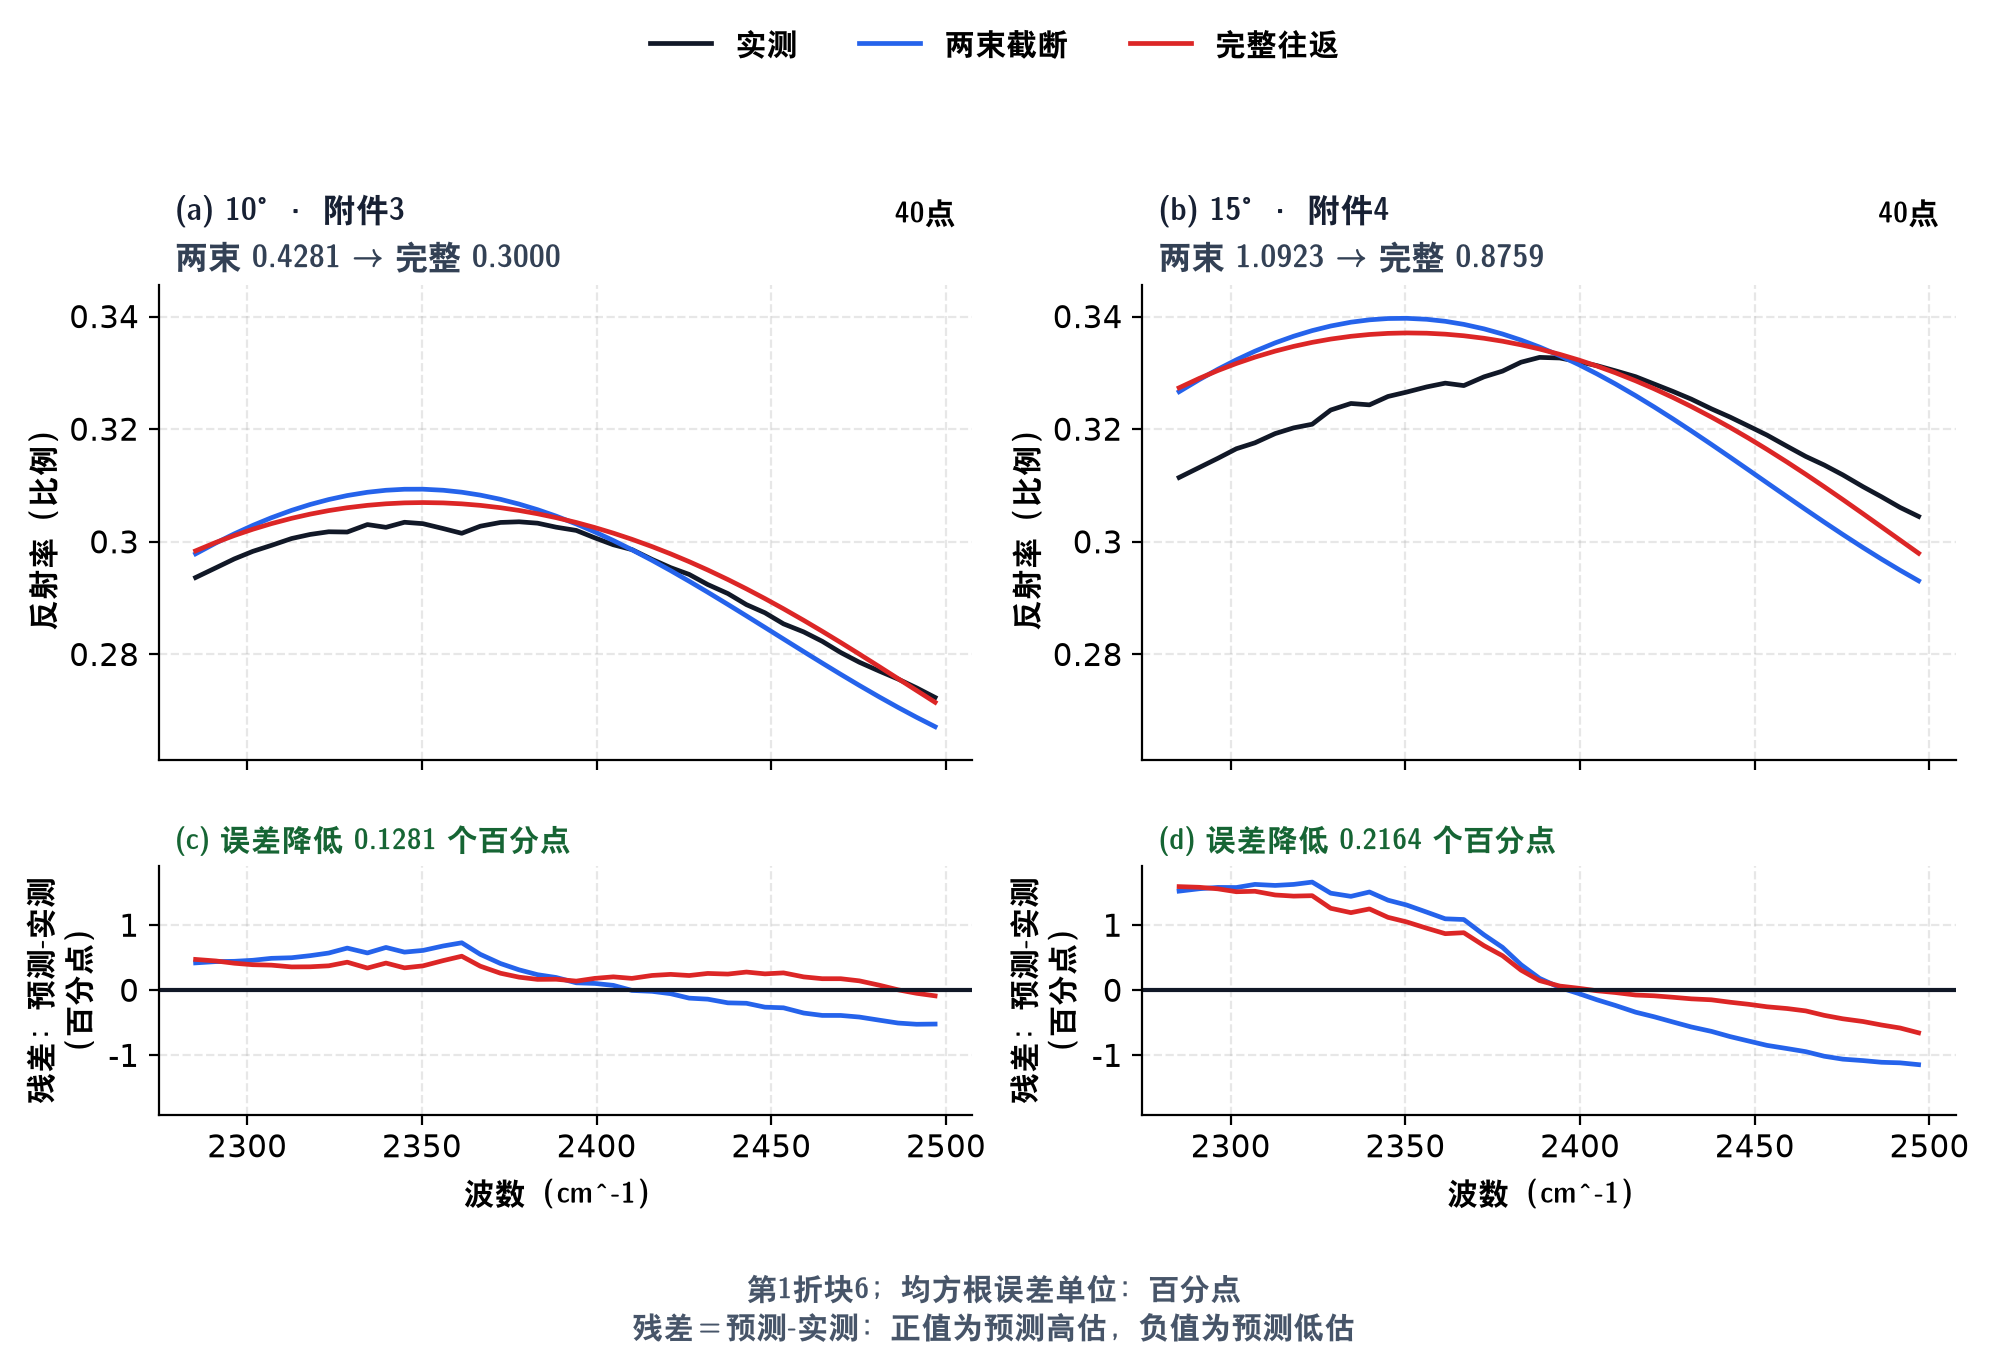
\includegraphics[width=0.8\textwidth]{../求解/问题3/图片/硅双角谱检验高阶贡献.png}
  \caption{硅两角高阶场预测残差存在差异}
  \label{fig:16}
\end{figure}
\endgroup

逐附件核对发现，硅附件三、四的高阶方案各在$2/4$个测试块上改善。早期对照曾因总体误差较低而保留完整往返，逐块检查却发现硅附件三仍有反向区段，因此保留各块的正负差值，表\ref{tab:supp-q3-blocks}与图\ref{fig:17}分别承担数值核对和方向比较。
% src:求解/问题3/结果/回炉轮3候选/仲裁闭环/20260910_131501_81623_建模公式/厚度结果.json:分材料验证.硅.逐角逐折逐块.0.完整相对两束下降_%;分材料验证.硅.逐角逐折逐块.1.完整相对两束下降_%;分材料验证.硅.逐角逐折逐块.2.完整相对两束下降_%;分材料验证.硅.逐角逐折逐块.3.完整相对两束下降_%;分材料验证.硅.逐角逐折逐块.4.完整相对两束下降_%;分材料验证.硅.逐角逐折逐块.5.完整相对两束下降_%;分材料验证.硅.逐角逐折逐块.6.完整相对两束下降_%;分材料验证.硅.逐角逐折逐块.7.完整相对两束下降_%
% src:交接/实验记录.json:852.类别;852.尝试;852.现象;852.决定

\begingroup
\setlength{\intextsep}{2pt}
\captionsetup{skip=3pt}
\begin{figure}[!htb]
  \centering
  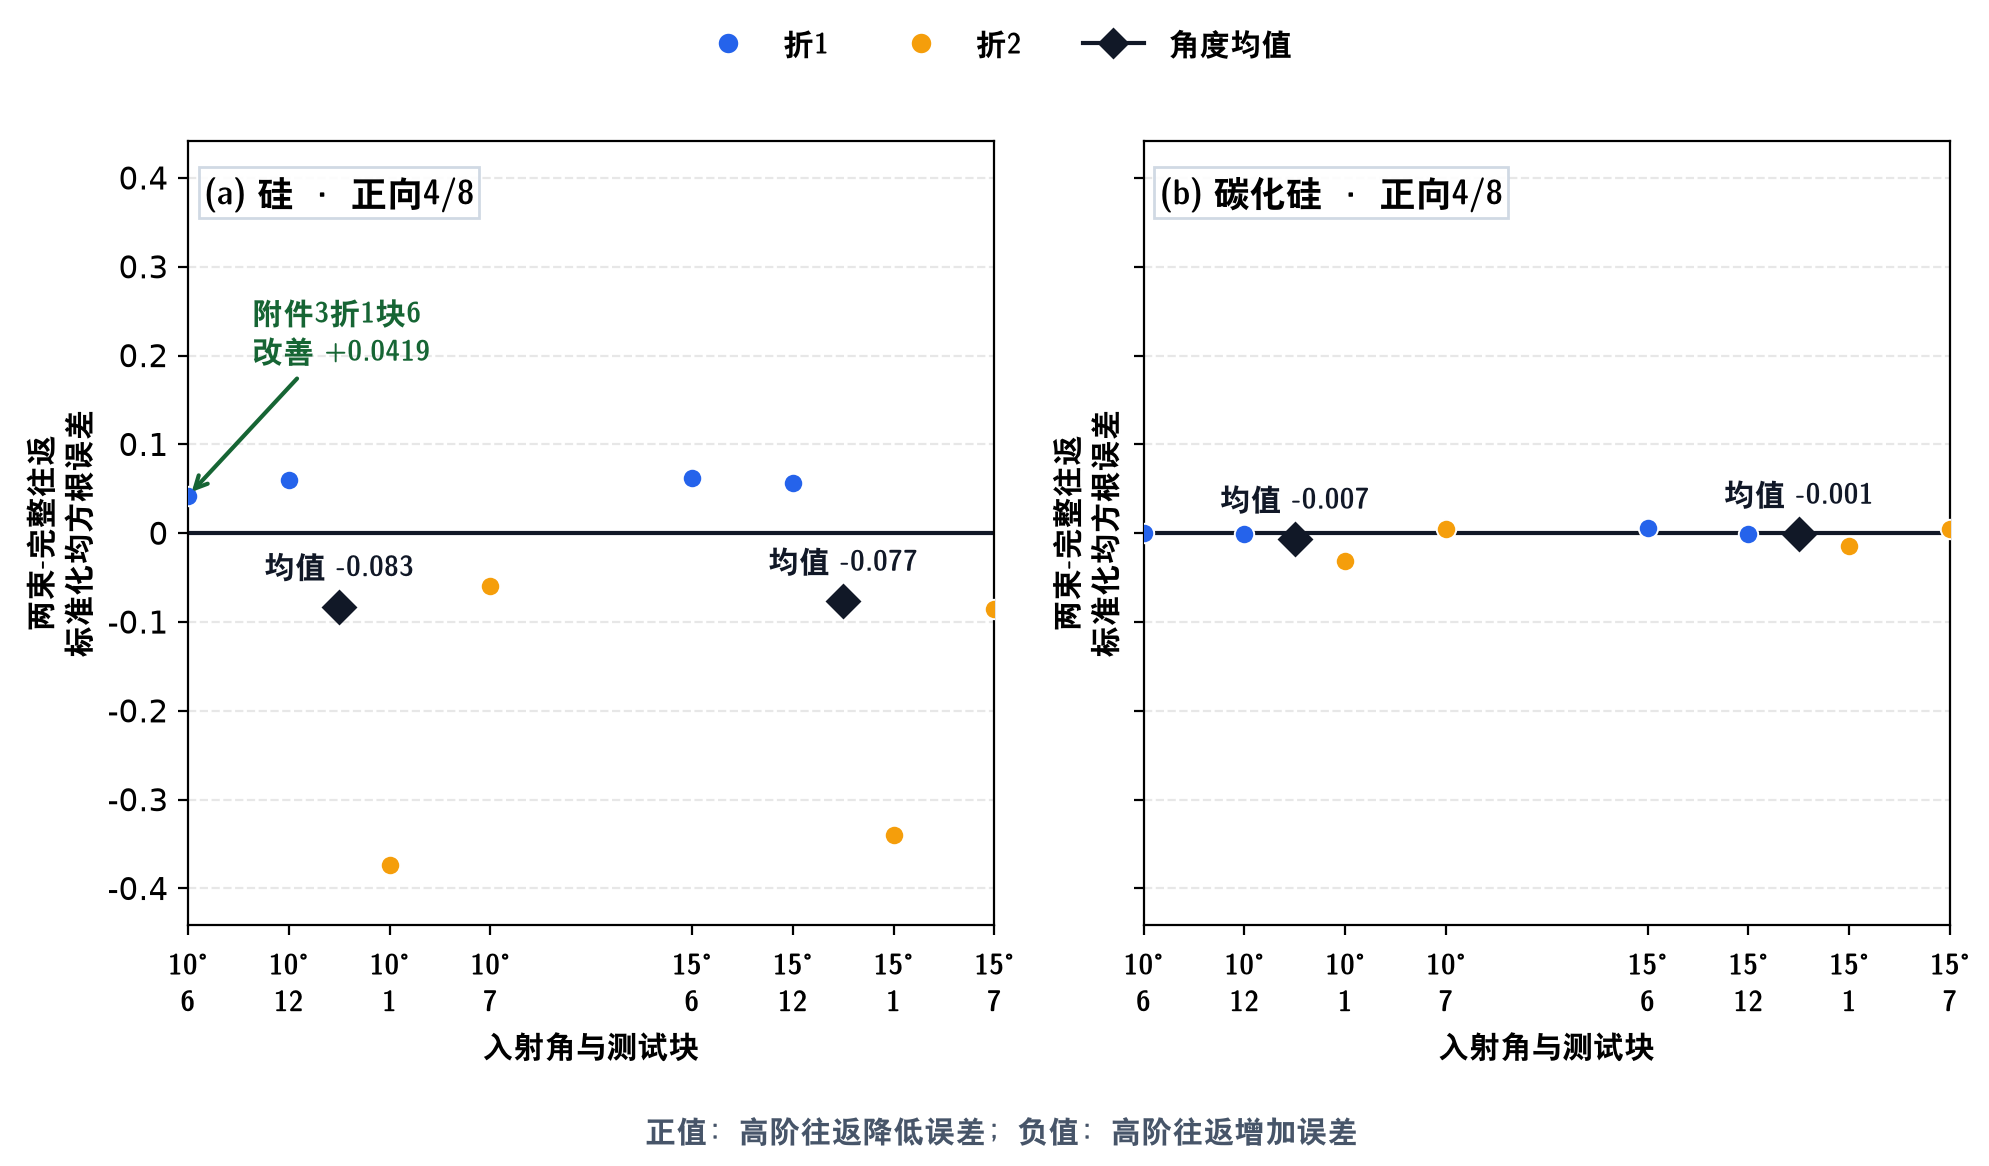
\includegraphics[width=0.8\textwidth]{../求解/问题3/图片/逐块对照区分两材料收益.png}
  \caption{两材料完整往返场的逐块误差改善}
  \label{fig:17}
\end{figure}
\endgroup

碳化硅附件一、二各有$2/4$个测试块出现高阶方案改善，正向收益均未贯穿全部区段。表\ref{tab:07}列出的物理可观测性与这些预测差异是两类证据。前者逐项检验式\eqref{eq:q3-cross-conditions}至式\eqref{eq:q3-resolution}的独立条件；后者比较留出光谱的预测误差。
% src:求解/问题3/结果/回炉轮3候选/仲裁闭环/20260910_131501_81623_建模公式/厚度结果.json:分材料验证.碳化硅.逐角逐折逐块.0.完整相对两束下降_%;分材料验证.碳化硅.逐角逐折逐块.1.完整相对两束下降_%;分材料验证.碳化硅.逐角逐折逐块.2.完整相对两束下降_%;分材料验证.碳化硅.逐角逐折逐块.3.完整相对两束下降_%;分材料验证.碳化硅.逐角逐折逐块.4.完整相对两束下降_%;分材料验证.碳化硅.逐角逐折逐块.5.完整相对两束下降_%;分材料验证.碳化硅.逐角逐折逐块.6.完整相对两束下降_%;分材料验证.碳化硅.逐角逐折逐块.7.完整相对两束下降_%

正向块并存负向块，说明高阶方案的预测收益没有贯穿四个附件。全量拟合中，硅与碳化硅的往返倍率模上界分别为$0.1441$和$0.0271$；表\ref{tab:q3-attachment-conditions}将这些模型内的非零返回与仍需测量的观测条件分列，不能从收敛直接跳到实验检出。
% src:求解/问题3/结果/公平对照.json:案例.0.场级数核验.最大往返乘子模;案例.3.场级数核验.最大往返乘子模

\begingroup
\footnotesize
\begin{longtable}{>{\centering\arraybackslash}p{0.06\textwidth}>{\centering\arraybackslash}p{0.12\textwidth}>{\centering\arraybackslash}p{0.19\textwidth}>{\centering\arraybackslash}p{0.20\textwidth}>{\centering\arraybackslash}p{0.27\textwidth}}
\caption{四附件的返回场与可观测条件}\label{tab:q3-attachment-conditions}\\
\hline
附件 & 正向块/总块 & 模型内可确认 & 谱形相容证据 & 未知观测条件\\
\hline
一 & $2/4$ & 非零返回、收敛 & 仅部分区段改善 & 相干、重叠、分辨及噪声\\
二 & $2/4$ & 非零返回、收敛 & 仅部分区段改善 & 相干、重叠、分辨及噪声\\
三 & $2/4$ & 非零返回、收敛 & 仅部分区段改善 & 相干、重叠、分辨及噪声\\
四 & $2/4$ & 非零返回、收敛 & 仅部分区段改善 & 相干、重叠、分辨及噪声\\
\hline
\end{longtable}
\endgroup
% src:求解/问题3/结果/回炉轮3候选/仲裁闭环/20260910_131501_81623_建模公式/厚度结果.json:分材料验证.硅.逐角逐折逐块.0.完整相对两束下降_%;分材料验证.硅.逐角逐折逐块.1.完整相对两束下降_%;分材料验证.硅.逐角逐折逐块.2.完整相对两束下降_%;分材料验证.硅.逐角逐折逐块.3.完整相对两束下降_%;分材料验证.硅.逐角逐折逐块.4.完整相对两束下降_%;分材料验证.硅.逐角逐折逐块.5.完整相对两束下降_%;分材料验证.硅.逐角逐折逐块.6.完整相对两束下降_%;分材料验证.硅.逐角逐折逐块.7.完整相对两束下降_%;分材料验证.碳化硅.逐角逐折逐块.0.完整相对两束下降_%;分材料验证.碳化硅.逐角逐折逐块.1.完整相对两束下降_%;分材料验证.碳化硅.逐角逐折逐块.2.完整相对两束下降_%;分材料验证.碳化硅.逐角逐折逐块.3.完整相对两束下降_%;分材料验证.碳化硅.逐角逐折逐块.4.完整相对两束下降_%;分材料验证.碳化硅.逐角逐折逐块.5.完整相对两束下降_%;分材料验证.碳化硅.逐角逐折逐块.6.完整相对两束下降_%;分材料验证.碳化硅.逐角逐折逐块.7.完整相对两束下降_%
% src:求解/问题3/结果/条件判定.json:必要条件

表中的非零返回与收敛均在所设光学模型内成立，相位关联、光束重叠和仪器响应则没有独立测量。图\ref{fig:roundtrip}中的返回路径对应$Bu$，相干叠加对应$\gamma_{mn}\eta_{mn}$；场幅逐次衰减本身不能确定卷积后的高阶交叉项是否高于噪声。

厚度影响也须单独识别。碳化硅同段厚度从$2.79$变为$2.83\ \mu\mathrm{m}$，折射率与损耗也同时改变，差值混合了参数补偿和往返影响。因此表\ref{tab:08}将模型对照与实际采用值分行。
% src:求解/问题3/结果/回炉轮3候选/仲裁闭环/20260910_131501_81623_建模公式/厚度结果.json:案例.6.最优.厚度_um;案例.7.最优.厚度_um;案例.6.最优.参数向量.1;案例.7.最优.参数向量.1;案例.6.最优.参数向量.4;案例.7.最优.参数向量.4

历史参数扰动中，碳化硅厚度变化介于$-1.6720$与$2.1261\ \mu\mathrm{m}$；图\ref{fig:19}保留这组重估对照，区别于固定参数的高阶场差，也未替换第二问的采用厚度。
% src:求解/问题3/结果/灵敏度.json:灵敏度_参数扰动.29.厚度变化_um;灵敏度_参数扰动.27.厚度变化_um;灵敏度_参数扰动.73.厚度变化_um;灵敏度_参数扰动.72.厚度变化_um

\begingroup
\setlength{\intextsep}{2pt}
\captionsetup{skip=3pt}

\endgroup

两项修正要求未同时成立，碳化硅维持$10.80\ \mu\mathrm{m}$及$0.64$--$18.11\ \mu\mathrm{m}$。图\ref{fig:20}并列两材料答案，硅的两折跨度与完整情景包络分开，碳化硅线段表示厚度重估范围。
% src:求解/问题3/结果/回炉轮3候选/仲裁闭环/20260910_131501_81623_建模公式/厚度结果.json:核心指标.碳化硅正式基准厚度_um;核心指标.碳化硅正式条件范围下限_um;核心指标.碳化硅正式条件范围上限_um
% src:求解/问题3/结果/条件判定.json:碳化硅条件分支.触发

\begingroup
\setlength{\intextsep}{2pt}
\captionsetup{skip=3pt}
\begin{figure}[!htb]
  \centering
  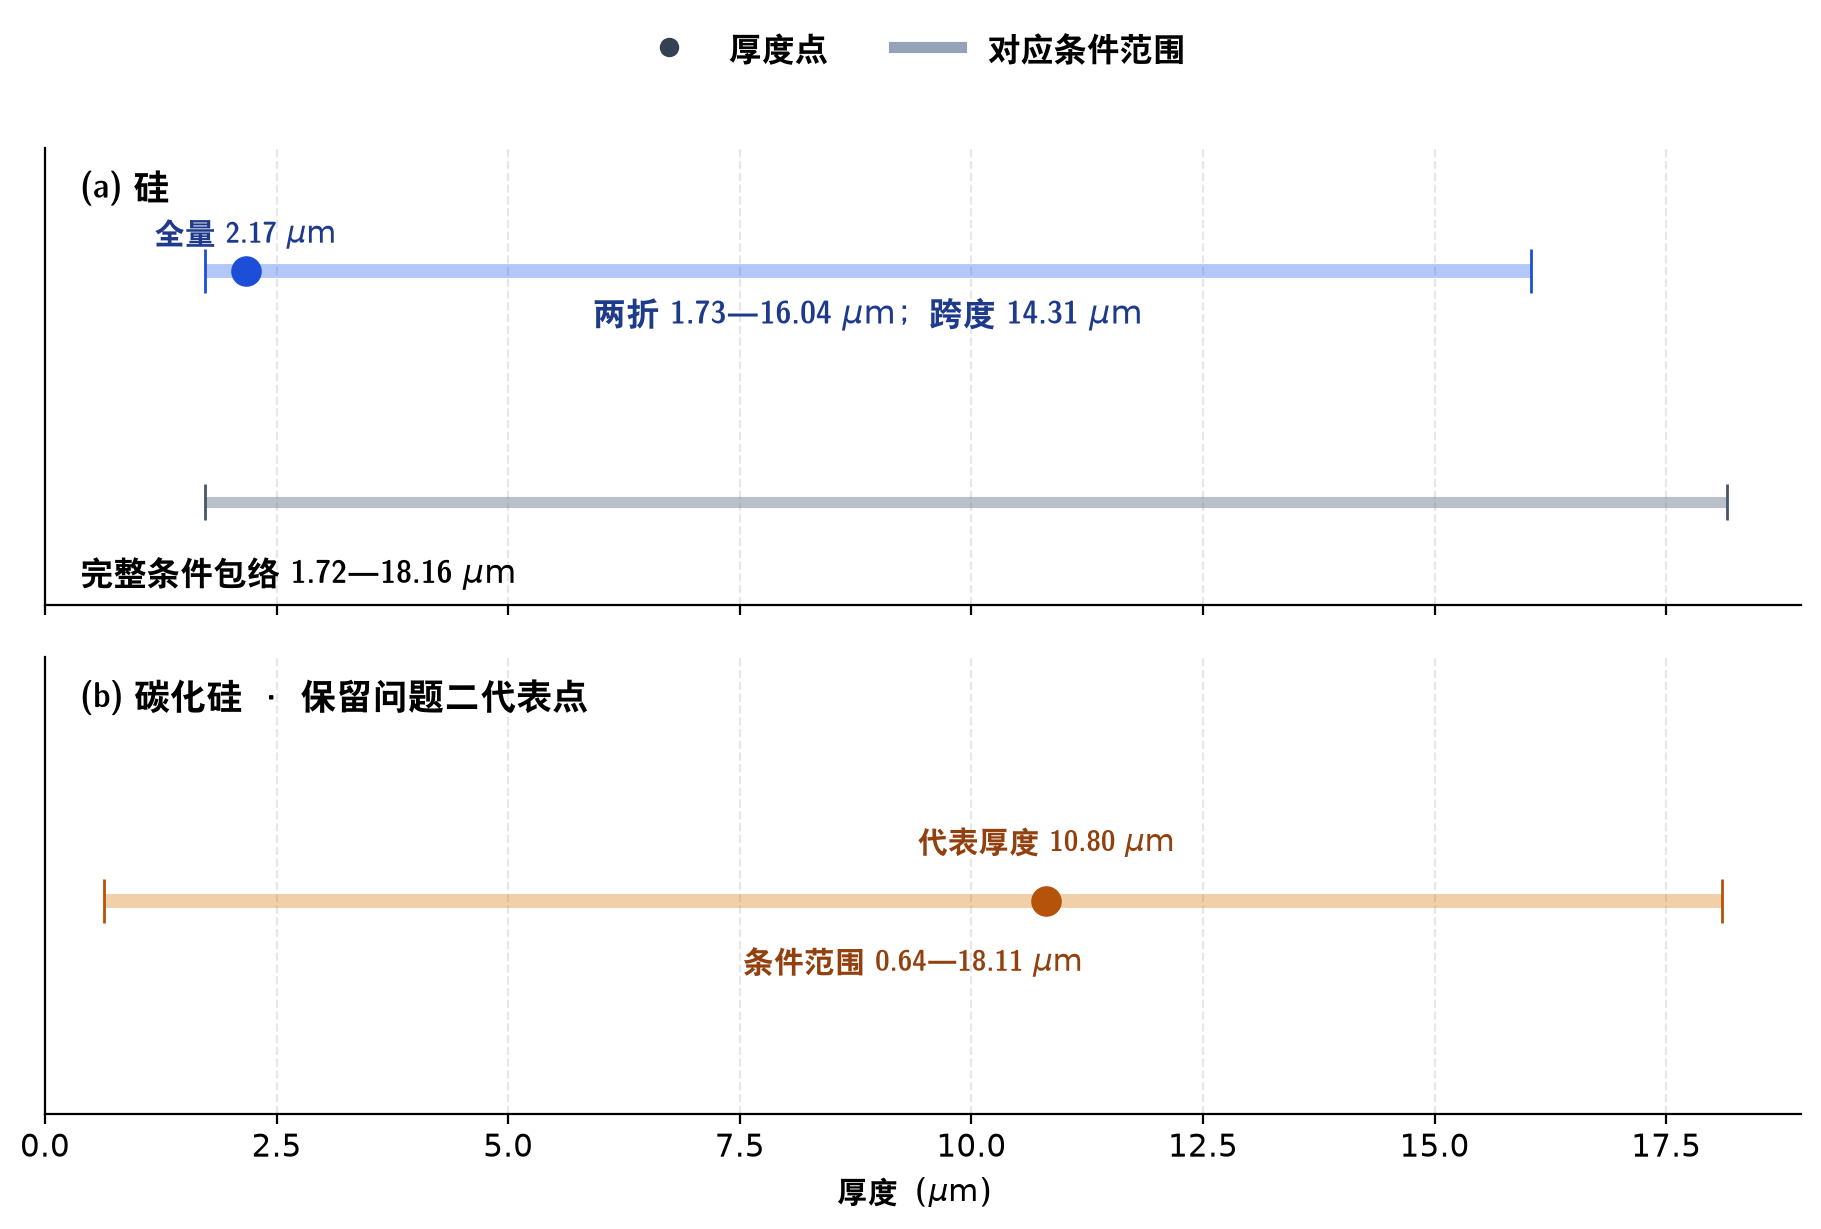
\includegraphics[width=0.8\textwidth]{../求解/问题3/图片/两材料厚度汇总保留条件.png}
  \caption{两材料厚度随切分与参数设置变化}
  \label{fig:20}
\end{figure}
\endgroup

硅采用完整往返场的全量拟合厚度，已计算的条件包络为$1.72$--$18.16\ \mu\mathrm{m}$，碳化硅沿用前问基准。包络由两模型全量、两折、近优候选及已算扰动的最外端点构成，是非概率的情景范围。
% src:求解/问题3/结果/回炉轮3候选/仲裁闭环/20260910_131501_81623_建模公式/厚度结果.json:核心指标.硅全量完整往返厚度_um;核心指标.硅折1完整往返条件厚度_um;核心指标.硅折2完整往返条件厚度_um;核心指标.硅已计算条件包络下限_um;核心指标.硅已计算条件包络上限_um;核心指标.碳化硅正式基准厚度_um;核心指标.碳化硅正式条件范围下限_um;核心指标.碳化硅正式条件范围上限_um

本问置信等级为低：硅次折相对训练均值劣化$11.30\%$，相对两束劣化$9.52\%$，两材料高阶收益跨折反向；同起点且均收敛的衬底扰动使厚度下降$13.83\%$，其他扰动的竞争分支差值跨零。已有结果给出有限光学条件下的最佳估计及描述性包络；已用于模型开发的测试区段承担探索性核对，独立同条件复算仍待补全，故尚不能确定唯一真厚度或概率区间。
% src:求解/问题3/结果/解读核验_回炉3_仲裁后.json:自检指标.硅折2相对训练均值改善_百分比;自检指标.硅折2相对两束改善_百分比;灵敏度.示例相对控制变化_百分比
% src:交接/结果声明_问题3.json:置信.等级;置信.理由

完整场的反射率测试经验覆盖率为$73.91\%$，低于名义$90\%$。下一章将反射率预测误差与厚度误差分开检验。
% src:求解/问题3/结果/回炉轮3候选/仲裁闭环/20260910_131501_81623_建模公式/厚度结果.json:预测区间.4.经验覆盖率;预测区间.4.平均区间宽度_比例;预测区间.5.经验覆盖率;预测区间.5.平均区间宽度_比例;预测区间.6.经验覆盖率;预测区间.6.平均区间宽度_比例;预测区间.7.经验覆盖率;预测区间.7.平均区间宽度_比例;预测区间.20.经验覆盖率;预测区间.20.平均区间宽度_比例;预测区间.21.经验覆盖率;预测区间.21.平均区间宽度_比例;预测区间.22.经验覆盖率;预测区间.22.平均区间宽度_比例;预测区间.23.经验覆盖率;预测区间.23.平均区间宽度_比例;预测区间.36.经验覆盖率;预测区间.36.平均区间宽度_比例;预测区间.37.经验覆盖率;预测区间.37.平均区间宽度_比例;预测区间.38.经验覆盖率;预测区间.38.平均区间宽度_比例;预测区间.39.经验覆盖率;预测区间.39.平均区间宽度_比例;预测区间.52.经验覆盖率;预测区间.52.平均区间宽度_比例;预测区间.53.经验覆盖率;预测区间.53.平均区间宽度_比例;预测区间.54.经验覆盖率;预测区间.54.平均区间宽度_比例;预测区间.55.经验覆盖率;预测区间.55.平均区间宽度_比例;预测区间.4.名义覆盖率
% src:求解/问题3/结果/回炉轮3候选/仲裁闭环/20260910_131501_81623_建模公式/厚度结果.json:逐块评分.4.测试点数;逐块评分.5.测试点数;逐块评分.6.测试点数;逐块评分.7.测试点数;逐块评分.20.测试点数;逐块评分.21.测试点数;逐块评分.22.测试点数;逐块评分.23.测试点数;逐块评分.36.测试点数;逐块评分.37.测试点数;逐块评分.38.测试点数;逐块评分.39.测试点数;逐块评分.52.测试点数;逐块评分.53.测试点数;逐块评分.54.测试点数;逐块评分.55.测试点数
% src:交接/结果声明_问题3.json:置信.等级;置信.理由

\par\endgroup

\section{模型检验：把拟合误差与测厚误差分开}

前章保留硅的完整往返场厚度与碳化硅的两束模型基准，本章分别核对反射率预测表现及厚度随光学条件的变化。

匹配合成数据的厚度平均绝对相对误差为$0.0008\%$（表\ref{tab:04}）；正式谱形分数在问题二为$1.2074$（表\ref{tab:q2-results}）、问题三为$1.0231$（表\ref{tab:08}），均无量纲。前者以合成光谱的已知厚度为参照，后两者以留出反射率为参照，分别评价厚度恢复与曲线预测。
% src:求解/问题1/结果/合成验证.json:主指标.数值
% src:求解/问题2/结果/验证.json:正式主方法分数_连续留段标准化均方根误差
% src:求解/问题3/结果/回炉轮3候选/仲裁闭环/20260910_131501_81623_建模公式/厚度结果.json:分材料验证.硅.逐折汇总.0.平均标准化均方根误差.两束;分材料验证.硅.逐折汇总.0.平均标准化均方根误差.完整往返;分材料验证.硅.逐折汇总.0.平均标准化均方根误差.训练均值;分材料验证.硅.逐折汇总.0.平均标准化均方根误差.二次趋势;分材料验证.硅.逐折汇总.1.平均标准化均方根误差.两束;分材料验证.硅.逐折汇总.1.平均标准化均方根误差.完整往返;分材料验证.硅.逐折汇总.1.平均标准化均方根误差.训练均值;分材料验证.硅.逐折汇总.1.平均标准化均方根误差.二次趋势;分材料验证.碳化硅.逐折汇总.0.平均标准化均方根误差.两束;分材料验证.碳化硅.逐折汇总.0.平均标准化均方根误差.完整往返;分材料验证.碳化硅.逐折汇总.0.平均标准化均方根误差.训练均值;分材料验证.碳化硅.逐折汇总.0.平均标准化均方根误差.二次趋势;分材料验证.碳化硅.逐折汇总.1.平均标准化均方根误差.两束;分材料验证.碳化硅.逐折汇总.1.平均标准化均方根误差.完整往返;分材料验证.碳化硅.逐折汇总.1.平均标准化均方根误差.训练均值;分材料验证.碳化硅.逐折汇总.1.平均标准化均方根误差.二次趋势

曲线预测仍有覆盖缺口：问题二测试覆盖率为$49.06\%$，低于$75\%$校准分位水平；问题三为$73.91\%$，低于$90\%$名义目标。图\ref{fig:q2-coverage}按观测点统计反射率预测区间的实际覆盖，再与各自的校准分位或名义目标比较。
% src:求解/问题2/结果/区间覆盖.json:测试经验覆盖率;校准经验分位点;构造方法
% src:求解/问题3/结果/回炉轮3候选/仲裁闭环/20260910_131501_81623_建模公式/厚度结果.json:预测区间.4.经验覆盖率;预测区间.4.平均区间宽度_比例;预测区间.5.经验覆盖率;预测区间.5.平均区间宽度_比例;预测区间.6.经验覆盖率;预测区间.6.平均区间宽度_比例;预测区间.7.经验覆盖率;预测区间.7.平均区间宽度_比例;预测区间.20.经验覆盖率;预测区间.20.平均区间宽度_比例;预测区间.21.经验覆盖率;预测区间.21.平均区间宽度_比例;预测区间.22.经验覆盖率;预测区间.22.平均区间宽度_比例;预测区间.23.经验覆盖率;预测区间.23.平均区间宽度_比例;预测区间.36.经验覆盖率;预测区间.36.平均区间宽度_比例;预测区间.37.经验覆盖率;预测区间.37.平均区间宽度_比例;预测区间.38.经验覆盖率;预测区间.38.平均区间宽度_比例;预测区间.39.经验覆盖率;预测区间.39.平均区间宽度_比例;预测区间.52.经验覆盖率;预测区间.52.平均区间宽度_比例;预测区间.53.经验覆盖率;预测区间.53.平均区间宽度_比例;预测区间.54.经验覆盖率;预测区间.54.平均区间宽度_比例;预测区间.55.经验覆盖率;预测区间.55.平均区间宽度_比例;预测区间.4.名义覆盖率
% src:求解/问题3/结果/回炉轮3候选/仲裁闭环/20260910_131501_81623_建模公式/厚度结果.json:逐块评分.4.测试点数;逐块评分.5.测试点数;逐块评分.6.测试点数;逐块评分.7.测试点数;逐块评分.20.测试点数;逐块评分.21.测试点数;逐块评分.22.测试点数;逐块评分.23.测试点数;逐块评分.36.测试点数;逐块评分.37.测试点数;逐块评分.38.测试点数;逐块评分.39.测试点数;逐块评分.52.测试点数;逐块评分.53.测试点数;逐块评分.54.测试点数;逐块评分.55.测试点数

光学条件扰动后，问题一固定合成样本的厚度重估为$6.66$--$10.01\,\mu\mathrm{m}$；问题二合并切分、剖面与参数情景，范围为$0.64$--$18.11\,\mu\mathrm{m}$（图\ref{fig:q2-thickness}）。这些跨度记录厚度与光学参数的相互补偿，硅另考察连续区段差异，碳化硅沿用问题二基准。以下两小节先厘清误差参照，再追问厚度为何随重估改变。
% src:求解/问题1/结果/灵敏度.json:条件压力范围_微米
% src:求解/问题2/结果/厚度结果.json:条件区间_微米
% src:求解/问题3/结果/回炉轮3候选/仲裁闭环/20260910_131501_81623_建模公式/厚度结果.json:核心指标.硅折1完整往返条件厚度_um;核心指标.硅折2完整往返条件厚度_um;核心指标.碳化硅正式基准厚度_um

\subsection{误差分析：连续留段与经验覆盖}
\label{sec:error-analysis}

碳化硅的谱形预测有所改善，区间覆盖却出现缺口。误差检验先拆开这两件事，再用材料分项和合成回收辨明测厚误差的参照。

原型比较曾给出主方法误差 $1.1717$；改用相同连续留段复核后，正式误差为 $1.2074$，低于二次趋势的 $1.4404$，改善 $16.17\%$，故采用正式评分衡量预测增益。上述误差均为无量纲的标准化反射率均方根误差，图\ref{fig:q2-residual}中的局部残差对应这一比较。
% src:交接/实验记录.json:528.尝试;528.现象;528.决定
% src:求解/问题2/结果/验证.json:三路线原型对比.双角色散变投影;正式主方法分数_连续留段标准化均方根误差;正式二次趋势基线分数_连续留段标准化均方根误差;正式主方法相对正式二次趋势改善_百分比

预测增益没有消除漏盖：测试反射率仅有 $157/320$ 点落入预测区间，经验覆盖率为 $49.06\%$。它衡量留出观测落入区间的比例；图\ref{fig:q2-coverage}与表\ref{tab:09}将这一比例和区间宽度并列。问题二采用校准残差的 $75\%$ 分位确定半宽，再由留出的测试块统计实际覆盖。
% src:求解/问题2/结果/区间覆盖.json:测试经验覆盖率;测试点数;校准经验分位点;构造方法
% src:求解/问题2/结果/验证.json:分块

\begingroup
\small
\setlength{\LTpre}{0.35em}
\setlength{\LTpost}{0.35em}
\begin{longtable}{>{\centering\arraybackslash}p{0.15\textwidth}>{\centering\arraybackslash}p{0.14\textwidth}>{\centering\arraybackslash}p{0.14\textwidth}>{\centering\arraybackslash}p{0.15\textwidth}>{\centering\arraybackslash}p{0.12\textwidth}>{\centering\arraybackslash}p{0.10\textwidth}}
\caption{正式实测反射率的点覆盖与整块覆盖}\label{tab:09}\\
\toprule
对象 & 分位/名义 & 点覆盖 & 全宽均值 & 整块覆盖 & 漏盖点\\
\midrule
\endfirsthead
\toprule
对象 & 分位/名义 & 点覆盖 & 全宽均值 & 整块覆盖 & 漏盖点\\
\midrule
\endhead
碳化硅 & $75\%$/--- & $157/320$ & $0.7424$ & $3/8$ & $163$\\
两材料 & $90\%/90\%$ & $473/640$ & $3.0875$ & $9/16$ & $167$\\
\bottomrule
\end{longtable}
% src:求解/问题2/结果/区间覆盖.json:校准经验分位点;构造方法;测试经验覆盖率;测试点数
% src:求解/问题2/结果/验证.json:分块
% src:求解/问题3/结果/回炉轮3候选/仲裁闭环/20260910_131501_81623_建模公式/厚度结果.json:预测区间.4.经验覆盖率;预测区间.4.平均区间宽度_比例;预测区间.5.经验覆盖率;预测区间.5.平均区间宽度_比例;预测区间.6.经验覆盖率;预测区间.6.平均区间宽度_比例;预测区间.7.经验覆盖率;预测区间.7.平均区间宽度_比例;预测区间.20.经验覆盖率;预测区间.20.平均区间宽度_比例;预测区间.21.经验覆盖率;预测区间.21.平均区间宽度_比例;预测区间.22.经验覆盖率;预测区间.22.平均区间宽度_比例;预测区间.23.经验覆盖率;预测区间.23.平均区间宽度_比例;预测区间.36.经验覆盖率;预测区间.36.平均区间宽度_比例;预测区间.37.经验覆盖率;预测区间.37.平均区间宽度_比例;预测区间.38.经验覆盖率;预测区间.38.平均区间宽度_比例;预测区间.39.经验覆盖率;预测区间.39.平均区间宽度_比例;预测区间.52.经验覆盖率;预测区间.52.平均区间宽度_比例;预测区间.53.经验覆盖率;预测区间.53.平均区间宽度_比例;预测区间.54.经验覆盖率;预测区间.54.平均区间宽度_比例;预测区间.55.经验覆盖率;预测区间.55.平均区间宽度_比例;预测区间.4.名义覆盖率
% src:求解/问题3/结果/回炉轮3候选/仲裁闭环/20260910_131501_81623_建模公式/厚度结果.json:逐块评分.4.测试点数;逐块评分.5.测试点数;逐块评分.6.测试点数;逐块评分.7.测试点数;逐块评分.20.测试点数;逐块评分.21.测试点数;逐块评分.22.测试点数;逐块评分.23.测试点数;逐块评分.36.测试点数;逐块评分.37.测试点数;逐块评分.38.测试点数;逐块评分.39.测试点数;逐块评分.52.测试点数;逐块评分.53.测试点数;逐块评分.54.测试点数;逐块评分.55.测试点数
% src:求解/问题3/结果/回炉轮3候选/仲裁闭环/20260910_131501_81623_建模公式/厚度结果.json:预测区间.4.经验覆盖率;预测区间.4.平均区间宽度_比例;预测区间.5.经验覆盖率;预测区间.5.平均区间宽度_比例;预测区间.6.经验覆盖率;预测区间.6.平均区间宽度_比例;预测区间.7.经验覆盖率;预测区间.7.平均区间宽度_比例;预测区间.20.经验覆盖率;预测区间.20.平均区间宽度_比例;预测区间.21.经验覆盖率;预测区间.21.平均区间宽度_比例;预测区间.22.经验覆盖率;预测区间.22.平均区间宽度_比例;预测区间.23.经验覆盖率;预测区间.23.平均区间宽度_比例;预测区间.36.经验覆盖率;预测区间.36.平均区间宽度_比例;预测区间.37.经验覆盖率;预测区间.37.平均区间宽度_比例;预测区间.38.经验覆盖率;预测区间.38.平均区间宽度_比例;预测区间.39.经验覆盖率;预测区间.39.平均区间宽度_比例;预测区间.52.经验覆盖率;预测区间.52.平均区间宽度_比例;预测区间.53.经验覆盖率;预测区间.53.平均区间宽度_比例;预测区间.54.经验覆盖率;预测区间.54.平均区间宽度_比例;预测区间.55.经验覆盖率;预测区间.55.平均区间宽度_比例;预测区间.4.名义覆盖率
% src:求解/问题3/结果/回炉轮3候选/仲裁闭环/20260910_131501_81623_建模公式/厚度结果.json:逐块评分.4.测试点数;逐块评分.5.测试点数;逐块评分.6.测试点数;逐块评分.7.测试点数;逐块评分.20.测试点数;逐块评分.21.测试点数;逐块评分.22.测试点数;逐块评分.23.测试点数;逐块评分.36.测试点数;逐块评分.37.测试点数;逐块评分.38.测试点数;逐块评分.39.测试点数;逐块评分.52.测试点数;逐块评分.53.测试点数;逐块评分.54.测试点数;逐块评分.55.测试点数
\endgroup

表中全宽以反射率百分点计，两材料行合计硅与碳化硅的完整往返场预测。整块覆盖要求该块全部观测落入同一点预测带，漏盖点保留逐点预测失败的次数。此处统计的整块覆盖不是另构造的块同时预测带覆盖；连续谱点彼此相关，点覆盖与整块覆盖分别检验该点预测带在单个观测及整段观测上的表现。

材料分项揭示了总体均值掩盖的冲突。完整往返场误差 $1.0231$ 高于两束的 $0.9812$；硅附件三、四各有 $2$ 个负改善块。表\ref{tab:supp-q3-blocks}逐项保留差值，图\ref{fig:16}与图\ref{fig:17}分别展示局部残差和块间方向；局部优势没有转化为总体预测改善。
% src:求解/问题3/结果/回炉轮3候选/仲裁闭环/20260910_131501_81623_建模公式/厚度结果.json:分材料验证.硅.逐角逐折逐块.0.完整相对两束下降_%;分材料验证.硅.逐角逐折逐块.1.完整相对两束下降_%;分材料验证.硅.逐角逐折逐块.2.完整相对两束下降_%;分材料验证.硅.逐角逐折逐块.3.完整相对两束下降_%;分材料验证.硅.逐角逐折逐块.4.完整相对两束下降_%;分材料验证.硅.逐角逐折逐块.5.完整相对两束下降_%;分材料验证.硅.逐角逐折逐块.6.完整相对两束下降_%;分材料验证.硅.逐角逐折逐块.7.完整相对两束下降_%
% src:求解/问题3/结果/回炉轮3候选/仲裁闭环/20260910_131501_81623_建模公式/厚度结果.json:分材料验证.硅.逐折汇总.0.平均标准化均方根误差.两束;分材料验证.硅.逐折汇总.0.平均标准化均方根误差.完整往返;分材料验证.硅.逐折汇总.0.平均标准化均方根误差.训练均值;分材料验证.硅.逐折汇总.0.平均标准化均方根误差.二次趋势;分材料验证.硅.逐折汇总.1.平均标准化均方根误差.两束;分材料验证.硅.逐折汇总.1.平均标准化均方根误差.完整往返;分材料验证.硅.逐折汇总.1.平均标准化均方根误差.训练均值;分材料验证.硅.逐折汇总.1.平均标准化均方根误差.二次趋势;分材料验证.碳化硅.逐折汇总.0.平均标准化均方根误差.两束;分材料验证.碳化硅.逐折汇总.0.平均标准化均方根误差.完整往返;分材料验证.碳化硅.逐折汇总.0.平均标准化均方根误差.训练均值;分材料验证.碳化硅.逐折汇总.0.平均标准化均方根误差.二次趋势;分材料验证.碳化硅.逐折汇总.1.平均标准化均方根误差.两束;分材料验证.碳化硅.逐折汇总.1.平均标准化均方根误差.完整往返;分材料验证.碳化硅.逐折汇总.1.平均标准化均方根误差.训练均值;分材料验证.碳化硅.逐折汇总.1.平均标准化均方根误差.二次趋势

第三问原第三版往返场估计器在低损耗、强损耗和无高阶负对照的$9$例匹配情景中，最大厚度相对误差绝对值为$0.0521\%$，但近优条件包络仅有$1/9$包含真厚度。表\ref{tab:q3-known-thickness}保留全部已知厚度案例；这组固定光学参数检验衡量厚度搜索的回收能力，与现行候选整合后的实测结果分列。
% src:求解/问题3/结果/公平对照.json:已知厚度验证.完成匹配情景数;已知厚度验证.案例.0.相对误差_%;已知厚度验证.案例.1.相对误差_%;已知厚度验证.案例.2.相对误差_%;已知厚度验证.案例.3.相对误差_%;已知厚度验证.案例.4.相对误差_%;已知厚度验证.案例.5.相对误差_%;已知厚度验证.案例.6.相对误差_%;已知厚度验证.案例.7.相对误差_%;已知厚度验证.案例.8.相对误差_%;已知厚度验证.条件包络经验包含率

色散失配时，厚度相对误差绝对值分别为$3.71\%$、$8.96\%$和$7.35\%$。这组检验将估计模型中的色散设为零，偏差随之放大，说明匹配光学参数时的小回收误差不能代表光学关系失配时的测厚表现。
% src:求解/问题3/结果/公平对照.json:已知厚度验证.案例.9.相对误差_%;已知厚度验证.案例.10.相对误差_%;已知厚度验证.案例.11.相对误差_%;已知厚度验证.案例.9.口径

合成近优包络收集固定生成条件下训练目标接近最优的厚度解；实测多情景包络还联合区段切分和光学条件变化，构造对象不同。前者的真值包含比例是这组模拟的经验计数，后者没有实测厚度真值可供同样计数，二者均未建立概率覆盖保证。

模型失配也放大了问题一的厚度误差：平均绝对相对误差由 $0.0008\%$ 升至 $0.3028\%$（图\ref{fig:08}），共同匹配组的常折射率峰距基线失败 $0$ 次。该项检验与第三问的直接厚度回收分别报告。合成回收以已知厚度为参照核对求解过程，光学参数扰动则考察固定观测下的厚度变化，下节沿这一方向展开重估比较。
% src:求解/问题1/结果/合成验证.json:主指标.数值;分组汇总.模型失配.平均绝对相对误差_百分比;常折射率峰距基线.失败数

\subsection{灵敏度分析：重新估计后的厚度变化}
\label{sec:sensitivity-analysis}

问题一先固定同一组合成光谱，考察光学条件改变后厚度怎样移动，再将这一比较延伸至实测材料。每项扰动均重新估计厚度，其余未固定参数随之重估。

合成例在折射率、色散斜率、偏振、平滑和角度扰动下，厚度落在$6.66$--$10.01\,\mu\mathrm{m}$，最大绝对漂移为$2.01\,\mu\mathrm{m}$。双束界面场反演仍给出有限厚度，但未知光学条件足以使它发生微米量级移动。
% src:求解/问题1/结果/灵敏度.json:条件压力范围_微米;最大绝对漂移_微米;重估结果

实测碳化硅放大了厚度与折射率的互相补偿：切分、剖面和满足参数约束的情景合并后，厚度范围为$0.64$--$18.11\,\mu\mathrm{m}$；五折极差除以中位数为$0.7604$，无量纲。图\ref{fig:q2-thickness}分开呈现这些来源，问题三的碳化硅沿用同一范围。
% src:求解/问题2/结果/厚度结果.json:条件区间_微米;条件区间构造
% src:求解/问题2/结果/验证.json:五折跨切分稳定性.相对极差
% src:求解/问题3/结果/回炉轮3候选/仲裁闭环/20260910_131501_81623_建模公式/厚度结果.json:核心指标.碳化硅正式条件范围下限_um;核心指标.碳化硅正式条件范围上限_um

为分开光学变化与优化继续推进的影响，硅次折增加同起点的未扰动控制：控制厚度为$16.0477\,\mu\mathrm{m}$，衬底对比增加$20\%$后为$13.8276\,\mu\mathrm{m}$，扣除控制后的厚度变化为$-2.2201\,\mu\mathrm{m}$。两个终点均满足收敛标准，因而这对差值对应同一起点附近的光学条件响应。
% src:求解/问题3/结果/解读核验_回炉3_仲裁后.json:灵敏度.示例控制厚度_um;灵敏度.示例扰动厚度_um;灵敏度.示例扣控制变化_um;灵敏度.示例成对收敛
% src:求解/问题3/结果/回炉轮3候选/仲裁闭环/20260910_131501_81623_建模公式/厚度结果.json:同起点控制分解.0.情景
% src:交接/实验记录.json:1724.尝试;1724.现象;1724.决定

原第三版的参数扰动保留为历史对照：硅厚度变化$-0.4571$至$3.9259\,\mu\mathrm{m}$，碳化硅变化$-1.6720$至$2.1261\,\mu\mathrm{m}$。图\ref{fig:19}和表\ref{tab:10}保留这些相对原折基准的差值；它们没有扣除未扰动优化推进，与同起点控制差分别解释。
% src:求解/问题3/结果/灵敏度.json:灵敏度_参数扰动.29.厚度变化_um;灵敏度_参数扰动.27.厚度变化_um;灵敏度_参数扰动.73.厚度变化_um;灵敏度_参数扰动.72.厚度变化_um

\begingroup
\small
\setlength{\LTpre}{0.3em}
\setlength{\LTpost}{0.3em}
\begin{longtable}{>{\centering\arraybackslash}p{0.14\textwidth}>{\centering\arraybackslash}p{0.235\textwidth}>{\centering\arraybackslash}p{0.19\textwidth}>{\centering\arraybackslash}p{0.17\textwidth}>{\centering\arraybackslash}p{0.105\textwidth}}
\caption{扰动重估改变厚度与拟合损失}\label{tab:10}\\
\toprule
重估对象 & 扰动设置 & 厚度或差/$\mu\mathrm{m}$ & 训练损失 & 判断\\
\midrule
\endfirsthead
\toprule
重估对象 & 扰动设置 & 厚度或差/$\mu\mathrm{m}$ & 训练损失 & 判断\\
\midrule
\endhead
合成厚度 & 折射率曲线$\pm20\%$ & $6.66$--$10.01$ & --- & 分支移动\\
碳化硅厚度 & 原设置 & $10.80$ & $0.2747$ & 参照\\
碳化硅厚度 & 折射率$-3\%/+3\%$ & $8.21/7.96$ & $0.3384/0.3294$ & 分支移动\\
碳化硅厚度 & 窗口下/上界$+100$ & $11.41/8.89$ & $0.2005/0.3161$ & 分支移动\\
碳化硅厚度 & 网格$96\to192$点 & $13.53$ & $0.2744$ & 分支移动\\
硅历史差 & 光学、响应与窗口 & $-0.4571$--$3.9259$ & --- & 分支移动\\
碳化硅历史差 & 光学、响应与窗口 & $-1.6720$--$2.1261$ & --- & 分支移动\\
\bottomrule
\end{longtable}
% src:求解/问题1/结果/灵敏度.json:重估结果.1.缩放;重估结果.2.缩放;条件压力范围_微米
% src:求解/问题2/结果/验证.json:窗口与模型灵敏度.0;窗口与模型灵敏度.5;窗口与模型灵敏度.6;窗口与模型灵敏度.8;窗口与模型灵敏度.9;窗口与模型灵敏度.10
% src:求解/问题3/结果/灵敏度.json:灵敏度_参数扰动.29.厚度变化_um;灵敏度_参数扰动.27.厚度变化_um;灵敏度_参数扰动.73.厚度变化_um;灵敏度_参数扰动.72.厚度变化_um
% src:交接/实验记录.json:564.现象
\endgroup

网格加密使碳化硅厚度移动$25.27\%$，而原代表点的损失仅比补查最低值高$0.1167\%$。这是固定点集、模型和物理边界后的数值搜索变化，不能与改变光学假设的情景变化混称为同一种不确定性。表\ref{tab:q2-search-check}保留两类近优点及其边界状态。
% src:求解/问题2/结果/搜索补查.json:原网格到加密厚度变化_百分比;原代表相对最低损失差_百分比

表\ref{tab:10}中窗口移动以$\mathrm{cm}^{-1}$计，斜线前后逐项对应；不同窗口的损失对应不同点集。异常原值均在主拟合窗口外，保留原值并不改变拟合点集，故裁剪异常不能解释厚度改善。
% src:求解/问题2/结果/验证.json:窗口与模型灵敏度.0;窗口与模型灵敏度.8
% src:求解/问题2/结果/数据审查.json:质量处置

窗口比较曾沿用原波段，两种边界结果重合；因此改为各向内移动$100\,\mathrm{cm}^{-1}$，在既定训练成员与新窗口的交集上重估。两折按所移动的边界分别保留每角$273$或$292$个训练点，选段影响才得以分开。
% src:交接/实验记录.json:554.尝试;554.现象;555.现象;556.尝试
% src:求解/问题3/结果/灵敏度.json:灵敏度_参数扰动.15.请求固定参数值;灵敏度_参数扰动.16.请求固定参数值;灵敏度_参数扰动.15.训练源行;灵敏度_参数扰动.16.训练源行;灵敏度_参数扰动.36.训练源行;灵敏度_参数扰动.37.训练源行;灵敏度_参数扰动.57.训练源行;灵敏度_参数扰动.58.训练源行;灵敏度_参数扰动.78.训练源行;灵敏度_参数扰动.79.训练源行

光学与角度扰动取折射率$\pm3\%$、衬底对比及损耗$\pm20\%$、入射角$\pm0.5^\circ$，偏振分别取两种纯态。重估后，硅沿用完整往返场，碳化硅保留两束基准。厚度响应记录这些设置对估计的影响，窗口和网格比较则揭示分支移动；下一章据此评价方法与推广条件。
% src:求解/问题3/结果/灵敏度.json:灵敏度_参数扰动.7.情景;灵敏度_参数扰动.8.情景;灵敏度_参数扰动.5.情景;灵敏度_参数扰动.6.情景;灵敏度_参数扰动.1.情景;灵敏度_参数扰动.2.情景;灵敏度_参数扰动.13.情景;灵敏度_参数扰动.14.情景;灵敏度_参数扰动.11.情景;灵敏度_参数扰动.12.情景
% src:交接/实验记录.json:564.现象

\section{模型评价与推广：数值答案及适用范围}

硅全量厚度为$2.17\,\mu\mathrm{m}$，非概率条件包络为$1.72$--$18.16\,\mu\mathrm{m}$。上一章的重估比较显示，厚度分支会随光学参数和窗口设置移动，本章据此评价双角约束的作用及后续标定方向。
% src:求解/问题3/结果/回炉轮3候选/仲裁闭环/20260910_131501_81623_建模公式/厚度结果.json:核心指标.硅全量完整往返厚度_um;核心指标.硅折1完整往返条件厚度_um;核心指标.硅折2完整往返条件厚度_um;核心指标.硅已计算条件包络下限_um;核心指标.硅已计算条件包络上限_um;核心指标.碳化硅正式基准厚度_um;核心指标.碳化硅正式条件范围下限_um;核心指标.碳化硅正式条件范围上限_um

碳化硅厚度为$10.80\,\mu\mathrm{m}$，厚度重估范围为$0.64$--$18.11\,\mu\mathrm{m}$（图\ref{fig:20}）。碳化硅沿用两束基准，未施加多光束修正（表\ref{tab:08}）。
% src:求解/问题3/结果/回炉轮3候选/仲裁闭环/20260910_131501_81623_建模公式/厚度结果.json:核心指标.硅全量完整往返厚度_um;核心指标.硅折1完整往返条件厚度_um;核心指标.硅折2完整往返条件厚度_um;核心指标.碳化硅正式基准厚度_um;核心指标.碳化硅正式条件范围下限_um;核心指标.碳化硅正式条件范围上限_um
% src:求解/问题3/结果/条件判定.json:碳化硅条件分支.触发

区段重估使硅厚度落在相距较远的分支；碳化硅的双角留段误差较二次趋势降低。完整往返场的高阶收益跨折反向，说明增加返回光并未稳定改善谱形预测。表\ref{tab:09}保留两问反射率测试覆盖的分子与分母，曲线预测区间仍有覆盖缺口。
% src:求解/问题3/结果/回炉轮3候选/仲裁闭环/20260910_131501_81623_建模公式/厚度结果.json:核心指标.硅折1完整往返条件厚度_um;核心指标.硅折2完整往返条件厚度_um
% src:求解/问题2/结果/验证.json:正式主方法相对正式二次趋势改善_百分比
% src:求解/问题3/结果/回炉轮3候选/仲裁闭环/20260910_131501_81623_建模公式/厚度结果.json:分材料验证.硅.逐折汇总.0.平均标准化均方根误差.两束;分材料验证.硅.逐折汇总.0.平均标准化均方根误差.完整往返;分材料验证.硅.逐折汇总.0.平均标准化均方根误差.训练均值;分材料验证.硅.逐折汇总.0.平均标准化均方根误差.二次趋势;分材料验证.硅.逐折汇总.1.平均标准化均方根误差.两束;分材料验证.硅.逐折汇总.1.平均标准化均方根误差.完整往返;分材料验证.硅.逐折汇总.1.平均标准化均方根误差.训练均值;分材料验证.硅.逐折汇总.1.平均标准化均方根误差.二次趋势;分材料验证.碳化硅.逐折汇总.0.平均标准化均方根误差.两束;分材料验证.碳化硅.逐折汇总.0.平均标准化均方根误差.完整往返;分材料验证.碳化硅.逐折汇总.0.平均标准化均方根误差.训练均值;分材料验证.碳化硅.逐折汇总.0.平均标准化均方根误差.二次趋势;分材料验证.碳化硅.逐折汇总.1.平均标准化均方根误差.两束;分材料验证.碳化硅.逐折汇总.1.平均标准化均方根误差.完整往返;分材料验证.碳化硅.逐折汇总.1.平均标准化均方根误差.训练均值;分材料验证.碳化硅.逐折汇总.1.平均标准化均方根误差.二次趋势
% src:求解/问题2/结果/区间覆盖.json:测试经验覆盖率
% src:求解/问题3/结果/回炉轮3候选/仲裁闭环/20260910_131501_81623_建模公式/厚度结果.json:预测区间.4.经验覆盖率;预测区间.4.平均区间宽度_比例;预测区间.5.经验覆盖率;预测区间.5.平均区间宽度_比例;预测区间.6.经验覆盖率;预测区间.6.平均区间宽度_比例;预测区间.7.经验覆盖率;预测区间.7.平均区间宽度_比例;预测区间.20.经验覆盖率;预测区间.20.平均区间宽度_比例;预测区间.21.经验覆盖率;预测区间.21.平均区间宽度_比例;预测区间.22.经验覆盖率;预测区间.22.平均区间宽度_比例;预测区间.23.经验覆盖率;预测区间.23.平均区间宽度_比例;预测区间.36.经验覆盖率;预测区间.36.平均区间宽度_比例;预测区间.37.经验覆盖率;预测区间.37.平均区间宽度_比例;预测区间.38.经验覆盖率;预测区间.38.平均区间宽度_比例;预测区间.39.经验覆盖率;预测区间.39.平均区间宽度_比例;预测区间.52.经验覆盖率;预测区间.52.平均区间宽度_比例;预测区间.53.经验覆盖率;预测区间.53.平均区间宽度_比例;预测区间.54.经验覆盖率;预测区间.54.平均区间宽度_比例;预测区间.55.经验覆盖率;预测区间.55.平均区间宽度_比例;预测区间.4.名义覆盖率
% src:求解/问题3/结果/回炉轮3候选/仲裁闭环/20260910_131501_81623_建模公式/厚度结果.json:逐块评分.4.测试点数;逐块评分.5.测试点数;逐块评分.6.测试点数;逐块评分.7.测试点数;逐块评分.20.测试点数;逐块评分.21.测试点数;逐块评分.22.测试点数;逐块评分.23.测试点数;逐块评分.36.测试点数;逐块评分.37.测试点数;逐块评分.38.测试点数;逐块评分.39.测试点数;逐块评分.52.测试点数;逐块评分.53.测试点数;逐块评分.54.测试点数;逐块评分.55.测试点数

现有双角观测缺少折射率曲线、相干长度及仪器分辨率标定。下文分别讨论双角约束的优点、光学参数互补的缺点，以及新增角度、标准厚度样片与光学标定的推广方向。
% src:交接/数据档案.json:总览.每块晶圆入射角度;未随附件提供的建模输入
% src:交接/结果声明_问题3.json:置信.理由

\subsection{优点：两角约束与可退化场模型}

同片双角应共同解释条纹，同时保留各自的响应差异。

共享厚度、逐角响应使条纹与背景分开解释。图\ref{fig:q2-residual}与表\ref{tab:q2-results}保留连续留段对照，避免逐角求厚度后平均。

场模型也能相互核对：直接取模平方与交叉项展开的最大差为$1.7\times10^{-16}$（反射率比例），图\ref{fig:field-expansion}验证了两种强度表达的一致性。
% src:求解/问题1/结果/模型验证.json:场展开一致性最大绝对差_比例

完整往返场沿用同一首返回场，往返振幅比趋零即退回两束。图\ref{fig:roundtrip}展示两模型的代数联系；分别估参的厚度差仍包含光学参数补偿。

测厚与高阶判断分开，图\ref{fig:20}与表\ref{tab:08}保留材料处理的区别，测厚不以检出高阶为前提。厚度与折射率的补偿、外部标定缺失，则是下节讨论的局限。

\subsection{缺点：光学参数互补与外部标定缺失}
\label{sec:limitations}

连续波段重估后的厚度仍然分散，厚度重估范围也随光学假设扩展。这使评价重点从曲线拟合好坏转向厚度是否被观测唯一确定。

碳化硅补充五折连续留段检验后，厚度分布于$5.53$--$13.51\,\mu\mathrm{m}$，极差与中位数之比为$0.7604$。部分分支超出原范围，因此将全部有效切分纳入范围；图\ref{fig:q2-thickness}保留了这种波段依赖。
% src:求解/问题2/结果/验证.json:五折跨切分稳定性.最小厚度_微米;五折跨切分稳定性.最大厚度_微米;五折跨切分稳定性.相对极差;五折跨切分稳定性.有效折数
% src:交接/实验记录.json:505.尝试;505.现象;505.决定

波段依赖反映厚度与未知折射率变化的互相补偿，即不同厚度也能配出相近条纹。纳入损失接近最小值的近优候选及参数扰动后，范围扩展至$0.64$--$18.11\,\mu\mathrm{m}$；这一跨度由已检验情景的最外端点确定，反映现有观测对厚度的约束较弱。
% src:求解/问题2/结果/厚度结果.json:条件区间_微米;条件区间组成

物理解释还受观测条件制约：相干性、空间重叠、仪器分辨率和偏振状态四类资料均缺失（表\ref{tab:07}）。完整往返场模型在部分区段改善谱形，总体误差却高于两束；物理可观测条件仍有缺项，碳化硅沿用问题二基准（图\ref{fig:20}）。
% src:求解/问题3/结果/条件判定.json:必要条件;碳化硅条件分支.触发
% src:交接/数据档案.json:未随附件提供的建模输入

区间覆盖也存在缺口：问题二、三的反射率测试经验覆盖率分别为$49.06\%$、$73.91\%$，前者低于$75\%$校准分位水平，后者低于$90\%$名义目标（图\ref{fig:q2-coverage}、表\ref{tab:09}）。校准残差给出的区间宽度未能充分容纳测试偏差，而真实附件的厚度真值也缺少独立参照。推广应从光学常数、标准厚度样片和重复测量补足这些缺口。
% src:求解/问题2/结果/区间覆盖.json:测试经验覆盖率;校准经验分位点
% src:求解/问题3/结果/回炉轮3候选/仲裁闭环/20260910_131501_81623_建模公式/厚度结果.json:预测区间.4.经验覆盖率;预测区间.4.平均区间宽度_比例;预测区间.5.经验覆盖率;预测区间.5.平均区间宽度_比例;预测区间.6.经验覆盖率;预测区间.6.平均区间宽度_比例;预测区间.7.经验覆盖率;预测区间.7.平均区间宽度_比例;预测区间.20.经验覆盖率;预测区间.20.平均区间宽度_比例;预测区间.21.经验覆盖率;预测区间.21.平均区间宽度_比例;预测区间.22.经验覆盖率;预测区间.22.平均区间宽度_比例;预测区间.23.经验覆盖率;预测区间.23.平均区间宽度_比例;预测区间.36.经验覆盖率;预测区间.36.平均区间宽度_比例;预测区间.37.经验覆盖率;预测区间.37.平均区间宽度_比例;预测区间.38.经验覆盖率;预测区间.38.平均区间宽度_比例;预测区间.39.经验覆盖率;预测区间.39.平均区间宽度_比例;预测区间.52.经验覆盖率;预测区间.52.平均区间宽度_比例;预测区间.53.经验覆盖率;预测区间.53.平均区间宽度_比例;预测区间.54.经验覆盖率;预测区间.54.平均区间宽度_比例;预测区间.55.经验覆盖率;预测区间.55.平均区间宽度_比例;预测区间.4.名义覆盖率
% src:求解/问题3/结果/回炉轮3候选/仲裁闭环/20260910_131501_81623_建模公式/厚度结果.json:逐块评分.4.测试点数;逐块评分.5.测试点数;逐块评分.6.测试点数;逐块评分.7.测试点数;逐块评分.20.测试点数;逐块评分.21.测试点数;逐块评分.22.测试点数;逐块评分.23.测试点数;逐块评分.36.测试点数;逐块评分.37.测试点数;逐块评分.38.测试点数;逐块评分.39.测试点数;逐块评分.52.测试点数;逐块评分.53.测试点数;逐块评分.54.测试点数;逐块评分.55.测试点数
% src:交接/数据档案.json:未随附件提供的建模输入

\subsection{推广：新增角度和标定可改善辨识}
\label{sec:extension}

双角约束仍难分开厚度与折射变化，推广应先补充观测，而非增加模型阶数。现有入射角只有$10^\circ$和$15^\circ$（图\ref{fig:overall-route}）；建议增加角度，借层内传播方向的差别（表\ref{tab:03}）检验各角度能否共用同一厚度和折射率曲线，冻结参数预测留出角度，用光谱误差衡量改进。
% src:交接/数据档案.json:总览.每块晶圆入射角度

标准厚度样片能为厚度提供外部参照。针对图\ref{fig:q2-thickness}、图\ref{fig:20}与表\ref{tab:10}中的分支分散，建议独立测定折射率与消光系数，用已知厚度约束往返衰减，再比较独立样片标定前后的厚度偏差，检验参数补偿是否减弱。

高阶项还需仪器观测支持。针对图\ref{fig:roundtrip}与表\ref{tab:07}，建议补测相干尺度、空间重叠、分辨率和偏振状态，再以同条件重复测量比较高阶谱形与噪声，用厚度离散程度检验重复性。这些均属后续实验建议，检验时以现有测厚结果为基准。
% src:交接/数据档案.json:未随附件提供的建模输入

\section{参考文献：薄膜光学与不确定性方法}
\label{sec:references}

前章提出光学标定与重复测量的方向，本节说明界面反射和区间检验的方法来源，区分物理推导与观测核对。空气、外延层和衬底构成三层介质，两种偏振的界面导纳及往返场在模型建立部分由边界条件和逐束叠加推出。表\ref{tab:available-info}与表\ref{tab:03}区分了观测给定量和待估参数；附件没有折射率曲线，通用光学关系中的材料参数保留为待估量。
% src:交接/数据档案.json:未随附件提供的建模输入

连续留段把相邻谱点保留在同一区段，再检查未参与拟合的光谱。问题二和问题三分别使用$320$个和$640$个测试点核对反射率预测区间，表\ref{tab:09}汇总其经验覆盖，即落入区间的测试点所占比例。以校准残差的经验分位构造区间的思路参照文献\cite{vovk2005conformal}；由于谱点连续相关，本文按留出点实计覆盖，检验对象是反射率预测，而非几何厚度。
% src:求解/问题2/结果/区间覆盖.json:测试点数;构造方法
% src:求解/问题3/结果/回炉轮3候选/仲裁闭环/20260910_131501_81623_建模公式/厚度结果.json:预测区间.4.经验覆盖率;预测区间.4.平均区间宽度_比例;预测区间.5.经验覆盖率;预测区间.5.平均区间宽度_比例;预测区间.6.经验覆盖率;预测区间.6.平均区间宽度_比例;预测区间.7.经验覆盖率;预测区间.7.平均区间宽度_比例;预测区间.20.经验覆盖率;预测区间.20.平均区间宽度_比例;预测区间.21.经验覆盖率;预测区间.21.平均区间宽度_比例;预测区间.22.经验覆盖率;预测区间.22.平均区间宽度_比例;预测区间.23.经验覆盖率;预测区间.23.平均区间宽度_比例;预测区间.36.经验覆盖率;预测区间.36.平均区间宽度_比例;预测区间.37.经验覆盖率;预测区间.37.平均区间宽度_比例;预测区间.38.经验覆盖率;预测区间.38.平均区间宽度_比例;预测区间.39.经验覆盖率;预测区间.39.平均区间宽度_比例;预测区间.52.经验覆盖率;预测区间.52.平均区间宽度_比例;预测区间.53.经验覆盖率;预测区间.53.平均区间宽度_比例;预测区间.54.经验覆盖率;预测区间.54.平均区间宽度_比例;预测区间.55.经验覆盖率;预测区间.55.平均区间宽度_比例;预测区间.4.名义覆盖率
% src:求解/问题3/结果/回炉轮3候选/仲裁闭环/20260910_131501_81623_建模公式/厚度结果.json:逐块评分.4.测试点数;逐块评分.5.测试点数;逐块评分.6.测试点数;逐块评分.7.测试点数;逐块评分.20.测试点数;逐块评分.21.测试点数;逐块评分.22.测试点数;逐块评分.23.测试点数;逐块评分.36.测试点数;逐块评分.37.测试点数;逐块评分.38.测试点数;逐块评分.39.测试点数;逐块评分.52.测试点数;逐块评分.53.测试点数;逐块评分.54.测试点数;逐块评分.55.测试点数

问题一的$19.54\,\mu\mathrm{m}$是周期等效量$T=5000/\Delta\sigma$，包含色散和界面相位变化的贡献，与后两问由光学模型求得的拟合厚度分列。各问的扰动比较记录厚度随光学条件的变化，文献提供通用方法，本题观测与模型计算支持样片结论。附录按问题列出计算材料、数据口径与完整比较，便于复核公式如何落实到观测与结果。
% src:求解/问题1/结果/模型验证.json:真实附件诊断.表观光学厚度乘积_dq_微米
% src:交接/结果声明_问题1.json:置信.等级;置信.理由
% src:交接/结果声明_问题2.json:置信.等级;置信.理由
% src:交接/结果声明_问题3.json:置信.等级;置信.理由

\begingroup
\renewcommand{\addcontentsline}[3]{}
\patchcmd{\thebibliography}{\section*{\refname}}{}{}{}
\begin{thebibliography}{9}
\bibitem{vovk2005conformal} Vovk V, Gammerman A, Shafer G. Algorithmic Learning in a Random World[M]. New York: Springer, 2005.
\end{thebibliography}
\endgroup

\section{附录：核心源码与补充数值}
\label{sec:appendix}

附录把正文的厚度答案、光场公式和对照结果放回各自的数据对象中，便于逐项复核。材料按两束场、同片双角估计和完整往返场的顺序展开，保留计算所需的输入约定与依赖，不用一串外部链接代替计算过程。

原始观测来自4个附件，每谱均有7469个共同波数点；附件的数量与独立晶圆的数量不是同一概念。表\ref{tab:app-products}按材料和计算任务列出产物，使相同名称的厚度结果能够对应到不同问题，而不是脱离点集与模型单独引用。
% src:交接/数据档案.json:总览.附件总数;总览.四文件共有波数点数

\begingroup
\small
\renewcommand{\arraystretch}{1.18}
\begin{longtable}{>{\centering\arraybackslash}p{0.18\textwidth}>{\centering\arraybackslash}p{0.34\textwidth}>{\centering\arraybackslash}p{0.40\textwidth}}
\caption{三问计算产物与复核对象}\label{tab:app-products}\\
\toprule
对象 & 产物名称 & 对应内容 \\
\midrule
\endfirsthead
\toprule
对象 & 产物名称 & 对应内容 \\
\midrule
\endhead
\bottomrule
\endfoot
原始观测 & 附件一至附件四工作簿 & 材料、角度、原始波数与反射率 \\
输入核对 & \texttt{\detokenize{数据档案.json}} & 附件标识、材料归属与单位 \\
合成条件 & \texttt{\detokenize{合成设计.json}} & 已知厚度情景及生成参数 \\
光学情景 & \texttt{\detokenize{路线侦察.json}} & 往返场初始情景及共同约束 \\
问题一 & \texttt{\detokenize{求解_问题1.py}} & 两束场、合成验证与周期诊断 \\
问题二 & \texttt{\detokenize{求解_问题2.py}} & 共同厚度、连续留段与条件范围 \\
问题三 & \texttt{\detokenize{求解_问题3.py}} & 同条件候选整合与两级精修 \\
问题一 & \texttt{\detokenize{模型验证.json}} & 两束展开、单位与真实谱周期 \\
问题一 & \texttt{\detokenize{合成验证.json}} & 已知厚度、失配情景与峰距对照 \\
问题一 & \texttt{\detokenize{独立角度切分验证.json}} & 整角度留出预测及逐例误差 \\
问题二 & \texttt{\detokenize{厚度结果.json}} & 同片厚度、逐折厚度与条件范围 \\
问题二 & \texttt{\detokenize{参数剖面.csv}} & 厚度与折射率的近等损失组合 \\
问题二 & \texttt{\detokenize{验证.json}} & 连续留段、留角度与基线对照 \\
问题二 & \texttt{\detokenize{基准交接.json}} & 向完整往返比较提供同片基准 \\
问题三 & \texttt{\detokenize{厚度结果.json}} & 全量硅厚度与碳化硅基准 \\
问题三 & \texttt{\detokenize{同口径对照.json}} & 逐块误差与有限级数核对 \\
问题三 & \texttt{\detokenize{条件判定.json}} & 逐附件支持与碳化硅处理依据 \\
问题二、三 & \texttt{\detokenize{留段预测.csv}} & 原始行号、观测与留出预测 \\
问题二、三 & \texttt{\detokenize{区间覆盖.json}} & 反射率覆盖的分母与构造 \\
问题二、三 & \texttt{\detokenize{灵敏度.csv}} & 参数及窗口扰动后的重新估计 \\
\end{longtable}
\endgroup

产物按各问所属目录区分，同名记录不相互替代。表中光谱预测误差检验的是曲线解释能力，合成厚度误差检验的是已知光学条件下的反演；两类检验分别保留，避免把曲线贴合程度当成真实晶圆的测厚精度。以下先核对一次返回场，再把共同厚度约束带入实测双角光谱。

问题一的两束场由界面直接反射和从衬底界面返回的部分组成，两者叠加产生条纹。早期尝试曾考虑直接用实测反射率评价绝对厚度误差，但附件没有厚度真值及折射率曲线，因此改用已知光学参数的合成光谱核对反演关系，并把真实光谱的周期诊断单独保留。
% src:交接/实验记录.json:22.尝试;22.现象;22.决定

真实谱的周期等效量为$19.54\,\mu\mathrm{m}$，而匹配合成情景的平均厚度相对误差为$0.0008\%$；它们分别回答条纹给出了什么量、给定光学条件后能否反推出厚度。表\ref{tab:app-q1}把场的代数核对与厚度比较分开，完整的计算内容见程序\ref{lst:q1-complete}。
% src:求解/问题1/结果/模型验证.json:真实附件诊断.表观光学厚度乘积_dq_微米
% src:求解/问题1/结果/合成验证.json:主指标.数值

\begingroup
\fontsize{8}{9}\selectfont
\renewcommand{\arraystretch}{1.00}
\setlength{\LTpre}{2pt}
\setlength{\LTpost}{2pt}
\begin{longtable}{>{\centering\arraybackslash}p{0.31\textwidth}>{\centering\arraybackslash}p{0.28\textwidth}>{\centering\arraybackslash}p{0.33\textwidth}}
\caption{两束场核对与合成误差分项}\label{tab:app-q1}\\
\toprule
核对对象 & 数值 & 数值含义 \\
\midrule
\endfirsthead
\toprule
核对对象 & 数值 & 数值含义 \\
\midrule
\endhead
\bottomrule
\endfoot
场强两种算法 & $1.6653\times10^{-16}$ & 反射率比例的最大绝对差 \\*
共同匹配情景 & $0.0008\%$ & 平均厚度绝对相对误差 \\*
新增匹配情景 & $0.0011\%$ & 平均厚度绝对相对误差 \\*
模型失配情景 & $0.3028\%$ & 平均厚度绝对相对误差 \\*
常折射率峰距 & $2.5875\%$ & 同组情景的朴素对照 \\*
双向整角度留出 & $0.0018\%$ & 留出厚度平均相对误差 \\*
合成锚例扰动 & $6.66$--$10.01\,\mu\mathrm{m}$ & 同一合成观测的重估范围 \\
\end{longtable}
% src:求解/问题1/结果/模型验证.json:场展开一致性最大绝对差_比例
% src:求解/问题1/结果/合成验证.json:主指标.数值;分组汇总.新增匹配.平均绝对相对误差_百分比;分组汇总.模型失配.平均绝对相对误差_百分比;常折射率峰距基线.平均绝对相对误差_百分比
% src:求解/问题1/结果/独立角度切分验证.json:留出指标.留出厚度预测平均绝对相对误差_百分比
% src:求解/问题1/结果/灵敏度.json:条件压力范围_微米
\endgroup

代数一致说明两种场强写法描述的是同一物理对象；失配情景则改变生成光谱的光学条件，检验问题从“计算是否一致”变成“假设改变后厚度如何移动”。因此程序保留两种强度写法、同型峰距基线和整角度留出，而非只展示最小的一项误差。

\begingroup
\lstset{basicstyle=\ttfamily\scriptsize,frame=single,numbers=left,stepnumber=5,numbersep=6pt,numberstyle=\tiny,breaklines=true,columns=fullflexible,keepspaces=true,showstringspaces=false,captionpos=t,xleftmargin=1.5em,linewidth=\dimexpr\linewidth-1.5em\relax,literate={≥}{{\ensuremath{\geq}}}1 {σ}{{\ensuremath{\sigma}}}1}
完整实现见清单\ref{lst:q1-complete}，此处不重复列出。
\endgroup

两束关系转入碳化硅实测谱后，需要让双角共同决定厚度和折射变化，同时让每个角度解释自己的慢变基线、振幅与固定相位。科学尝试比较了这种共享参数方式与逐角厚度简单平均，发现不同波段的反射率起伏差异明显，且缺少折射率曲线，因而保留共同物理参数和逐角低阶响应。
% src:交接/实验记录.json:34.尝试;34.现象;34.决定

问题二的$10.80\,\mu\mathrm{m}$来自每角480点的共同原坐标样本，并非主窗口全部原始点的另一名称。表\ref{tab:app-q2}同时列出点估计、两折及五折厚度，保持连续区段变化与整体拟合的对应关系。
% src:求解/问题2/结果/厚度结果.json:同片最佳厚度_微米
% src:求解/问题2/结果/数据审查.json:抽样点数_每角度

条件范围$0.64$--$18.11\,\mu\mathrm{m}$汇集了数据切分、厚度与折射率补偿关系及合法参数情景，含义是改变这些条件后得到的厚度跨度。它与共同样本的整体拟合并列，说明范围的构造比单次拟合多考虑了哪些变化。
% src:求解/问题2/结果/厚度结果.json:条件区间_微米;条件区间构造

\begingroup
\small
\begin{longtable}{>{\centering\arraybackslash}p{0.24\textwidth}>{\centering\arraybackslash}p{0.31\textwidth}>{\centering\arraybackslash}p{0.37\textwidth}}
\caption{碳化硅厚度按点集与范围分列}\label{tab:app-q2}\\
\toprule
对象 & 厚度$/\mu\mathrm{m}$ & 构造 \\
\midrule
\endfirsthead
\toprule
对象 & 厚度$/\mu\mathrm{m}$ & 构造 \\
\midrule
\endhead
\bottomrule
\endfoot
同片非触边代表 & $10.80$ & 原搜索代表，另保留触边候选 \\
两折连续留段 & $13.08,\ 10.65$ & 按各折训练区段重新估计 \\
五折连续留段 & $13.37,\ 10.49,\ 6.53$ & 前三折的独立拟合厚度 \\
五折连续留段 & $13.51,\ 5.53$ & 后两折的独立拟合厚度 \\
条件范围 & $0.64$--$18.11$ & 切分、剖面与合法情景并集 \\
\end{longtable}
% src:求解/问题2/结果/厚度结果.json:同片最佳厚度_微米;两折条件厚度_微米;五折条件厚度_微米;条件区间_微米;条件区间构造
\endgroup

厚度范围与反射率预测覆盖有不同的分母和解释对象。程序\ref{lst:q2-complete}将二者分别计算：厚度范围追踪物理参数随条件的变化，反射率覆盖核对留出光谱点是否落入预测带，后者不会被用来给前者附加概率含义。

\begingroup
\lstset{basicstyle=\ttfamily\scriptsize,frame=single,numbers=left,stepnumber=5,numbersep=6pt,numberstyle=\tiny,breaklines=true,columns=fullflexible,keepspaces=true,showstringspaces=false,captionpos=t,xleftmargin=1.5em,linewidth=\dimexpr\linewidth-1.5em\relax,literate={≥}{{\ensuremath{\geq}}}1 {σ}{{\ensuremath{\sigma}}}1}
完整实现见清单\ref{lst:q2-complete}，此处不重复列出。
\endgroup

共同样本的厚度与条件范围明确后，完整往返场的比较继续沿用相同留出区段，并另建硅的主窗口全量对象。所谓完整往返，就是在首个返回场之后，让后续每轮返回再乘同一衰减和相位因子，最后将所有返回场相加；截去后续返回便恢复两束关系。

硅的全量估计为$2.17\,\mu\mathrm{m}$，所用主窗口每角含5392个原始点。表\ref{tab:app-q3}将它与计划折分放在不同的行，避免把训练区段产生的厚度差异压缩成一个平均值。
% src:求解/问题3/结果/回炉轮3候选/仲裁闭环/20260910_131501_81623_建模公式/厚度结果.json:核心指标.硅全量完整往返厚度_um
% src:求解/问题3/结果/公平对照.json:案例.0.每角点数

计划折分每角480点，两次训练得到$1.73\,\mu\mathrm{m}$与$16.04\,\mu\mathrm{m}$，差别指向区段选择对厚度分支的影响。碳化硅保留$10.80\,\mu\mathrm{m}$基准，其共同样本与光学条件不会随硅全量对象的建立而改变。
% src:求解/问题3/结果/公平对照.json:案例.1.每角点数;案例.2.每角点数
% src:求解/问题3/结果/回炉轮3候选/仲裁闭环/20260910_131501_81623_建模公式/厚度结果.json:核心指标.硅折1完整往返条件厚度_um;核心指标.硅折2完整往返条件厚度_um;核心指标.碳化硅正式基准厚度_um

\begingroup
\small
\begin{longtable}{>{\centering\arraybackslash}p{0.21\textwidth}>{\centering\arraybackslash}p{0.19\textwidth}>{\centering\arraybackslash}p{0.24\textwidth}>{\centering\arraybackslash}p{0.24\textwidth}}
\caption{两材料厚度保留全量与折分区别}\label{tab:app-q3}\\
\toprule
材料与对象 & 点数/角 & 厚度$/\mu\mathrm{m}$ & 模型 \\
\midrule
\endfirsthead
\toprule
材料与对象 & 点数/角 & 厚度$/\mu\mathrm{m}$ & 模型 \\
\midrule
\endhead
\bottomrule
\endfoot
硅原始全量 & $5392$ & $2.17$ & 完整往返 \\
硅计划折分 & $480$ & $1.73,\ 16.04$ & 完整往返 \\
碳化硅基准 & $480$ & $10.80$ & 问题二两束 \\
碳化硅范围 & $480$ & $0.64$--$18.11$ & 问题二条件并集 \\
\end{longtable}
% src:求解/问题3/结果/公平对照.json:案例.0.每角点数;案例.1.每角点数;案例.2.每角点数
% src:求解/问题3/结果/回炉轮3候选/仲裁闭环/20260910_131501_81623_建模公式/厚度结果.json:核心指标.硅全量完整往返厚度_um;核心指标.硅折1完整往返条件厚度_um;核心指标.硅折2完整往返条件厚度_um;核心指标.碳化硅正式基准厚度_um;核心指标.碳化硅正式条件范围下限_um;核心指标.碳化硅正式条件范围上限_um
\endgroup

折间厚度的变化对应同一材料更换训练区段，材料之间的差别则对应不同晶圆，二者不能合成一条共同的误差范围。保留这两层区别后，完整往返场与两束场的优劣才有明确的比较对象。

同段比较时，完整往返的标准化反射率误差为1.0231，两束对照为0.9812；实际尝试同时发现硅十度谱存在负改善区段，因此程序保留逐块比较，不让总体平均掩盖局部反向变化。表\ref{tab:app-comparison}保留两问各自的基线尺度，程序\ref{lst:q3-complete}给出对应的往返求和、配对评分和材料处理分支。
% src:求解/问题3/结果/回炉轮3候选/仲裁闭环/20260910_131501_81623_建模公式/厚度结果.json:分材料验证.硅.逐折汇总.0.平均标准化均方根误差.两束;分材料验证.硅.逐折汇总.0.平均标准化均方根误差.完整往返;分材料验证.硅.逐折汇总.0.平均标准化均方根误差.训练均值;分材料验证.硅.逐折汇总.0.平均标准化均方根误差.二次趋势;分材料验证.硅.逐折汇总.1.平均标准化均方根误差.两束;分材料验证.硅.逐折汇总.1.平均标准化均方根误差.完整往返;分材料验证.硅.逐折汇总.1.平均标准化均方根误差.训练均值;分材料验证.硅.逐折汇总.1.平均标准化均方根误差.二次趋势;分材料验证.碳化硅.逐折汇总.0.平均标准化均方根误差.两束;分材料验证.碳化硅.逐折汇总.0.平均标准化均方根误差.完整往返;分材料验证.碳化硅.逐折汇总.0.平均标准化均方根误差.训练均值;分材料验证.碳化硅.逐折汇总.0.平均标准化均方根误差.二次趋势;分材料验证.碳化硅.逐折汇总.1.平均标准化均方根误差.两束;分材料验证.碳化硅.逐折汇总.1.平均标准化均方根误差.完整往返;分材料验证.碳化硅.逐折汇总.1.平均标准化均方根误差.训练均值;分材料验证.碳化硅.逐折汇总.1.平均标准化均方根误差.二次趋势
% src:交接/实验记录.json:563.尝试;563.现象;563.决定

\begingroup
\small
\begin{longtable}{>{\centering\arraybackslash}p{0.20\textwidth}>{\centering\arraybackslash}p{0.40\textwidth}>{\centering\arraybackslash}p{0.32\textwidth}}
\caption{连续留段误差按各问基线比较}\label{tab:app-comparison}\\
\toprule
问题 & 比较方法 & 标准化反射率误差 \\
\midrule
\endfirsthead
\toprule
问题 & 比较方法 & 标准化反射率误差 \\
\midrule
\endhead
\bottomrule
\endfoot
问题二 & 共享厚度两束模型 & $1.2074$ \\
问题二 & 二次趋势 & $1.4404$ \\
问题三 & 完整往返场 & $1.0231$ \\
问题三 & 两束截断场 & $0.9812$ \\
问题三 & 二次趋势 & $1.4434$ \\
问题三 & 训练均值 & $2.1929$ \\
\end{longtable}
% src:求解/问题2/结果/验证.json:正式主方法分数_连续留段标准化均方根误差;正式二次趋势基线分数_连续留段标准化均方根误差
% src:求解/问题3/结果/回炉轮3候选/仲裁闭环/20260910_131501_81623_建模公式/厚度结果.json:分材料验证.硅.逐折汇总.0.平均标准化均方根误差.两束;分材料验证.硅.逐折汇总.0.平均标准化均方根误差.完整往返;分材料验证.硅.逐折汇总.0.平均标准化均方根误差.训练均值;分材料验证.硅.逐折汇总.0.平均标准化均方根误差.二次趋势;分材料验证.硅.逐折汇总.1.平均标准化均方根误差.两束;分材料验证.硅.逐折汇总.1.平均标准化均方根误差.完整往返;分材料验证.硅.逐折汇总.1.平均标准化均方根误差.训练均值;分材料验证.硅.逐折汇总.1.平均标准化均方根误差.二次趋势;分材料验证.碳化硅.逐折汇总.0.平均标准化均方根误差.两束;分材料验证.碳化硅.逐折汇总.0.平均标准化均方根误差.完整往返;分材料验证.碳化硅.逐折汇总.0.平均标准化均方根误差.训练均值;分材料验证.碳化硅.逐折汇总.0.平均标准化均方根误差.二次趋势;分材料验证.碳化硅.逐折汇总.1.平均标准化均方根误差.两束;分材料验证.碳化硅.逐折汇总.1.平均标准化均方根误差.完整往返;分材料验证.碳化硅.逐折汇总.1.平均标准化均方根误差.训练均值;分材料验证.碳化硅.逐折汇总.1.平均标准化均方根误差.二次趋势
\endgroup

总体误差未下降，说明高阶返回没有带来整体预测改善；相干长度、光束空间重叠和仪器分辨率则回答这些返回能否在测量中形成可分辨干涉。两种问题分开计算和记录，碳化硅的处理仍使用问题二基准，逐附件判断和窗口扰动保留在相应产物中。

\begingroup
\lstset{basicstyle=\ttfamily\scriptsize,frame=single,numbers=left,stepnumber=5,numbersep=6pt,numberstyle=\tiny,breaklines=true,columns=fullflexible,keepspaces=true,showstringspaces=false,captionpos=t,xleftmargin=1.5em,linewidth=\dimexpr\linewidth-1.5em\relax,literate={≥}{{\ensuremath{\geq}}}1 {σ}{{\ensuremath{\sigma}}}1}
完整实现见清单\ref{lst:q3-complete}，此处不重复列出。
\endgroup

各问完整程序保留依赖导入、数据读取、核心函数和执行入口。问题三以清单\ref{lst:q3-current}为现行入口，调用清单\ref{lst:q3-complete}的基础引擎和清单\ref{lst:q3-independent}的独立公式；冻结输入及数值对应关系见清单\ref{lst:q3-products}。程序\ref{lst:app-run}列出前两问的执行命令；问题三保持现有附件与碳化硅基准不变，按清单\ref{lst:q3-run}隔离重算，基础引擎不再单独充当现行计算，复算也不自动覆盖本文结果。

\begingroup
\lstset{basicstyle=\ttfamily\footnotesize,frame=single,numbers=none,breaklines=true,captionpos=t}
\begin{lstlisting}[language=bash,caption={从工作根执行前两问计算},label={lst:app-run}]
python3 求解/问题1/求解_问题1.py
python3 求解/问题2/求解_问题2.py
\end{lstlisting}
\endgroup

这些计算入口将模型、点集和结果逐一对应，补充材料再据此展开源行索引、参数对照及逐块数值，而不改变正文已经给出的答案。

\subsection{问题一源码：两束场与合成验证}
\label{sec:appendix-q1}

一次往返场展开在本附录中保持原来的光路边界：外延层上表面的直接反射场，与进入外延层、到达衬底界面后返回的首束场相加。空气、外延层和衬底的界面关系沿用图\ref{fig:once-return}，角度与单位沿用表\ref{tab:03}；入射角分别为 $10^\circ$ 和 $15^\circ$，估计反射强度时不加入后续往返的分母。这样，合成检验与真实条纹诊断都从同一个一次返回模型出发。
% src:数据/问题1_冻结合成输入/合成设计.json:角度_度

直接求光场模平方与展开交叉项之间，最大绝对差为 $1.7\times10^{-16}$，以反射率比例计；厚度输入 $8\,\mu\mathrm{m}$ 时，内部换为 $0.0008\,\mathrm{cm}$，回换后厚度不变。图\ref{fig:field-expansion}中的逐点一致性与表\ref{tab:q1-appendix-checks}的基础核验相互对应，把代数展开和量纲换算分别落到可核对的量上。
% src:求解/问题1/结果/模型验证.json:场展开一致性最大绝对差_比例;单位换算.输入厚度_微米;单位换算.厚度_厘米;单位换算.回换厚度_微米

\begingroup
\small
\renewcommand{\arraystretch}{1.15}
\begin{longtable}{>{\centering\arraybackslash}p{0.30\textwidth}>{\centering\arraybackslash}p{0.31\textwidth}>{\centering\arraybackslash}p{0.31\textwidth}}
\caption{一次返回场的代数与量纲核验}\label{tab:q1-appendix-checks}\\
\toprule
核验对象 & 数值或关系 & 核对内容 \\
\midrule
\endfirsthead
\toprule
核验对象 & 数值或关系 & 核对内容 \\
\midrule
\endhead
\bottomrule
\endfoot
两种强度计算 & $1.7\times10^{-16}$ & 最大绝对差，比例 \\
零界面返回项 & $0$ & 退化差，比例 \\
厚度内部换算 & $8\,\mu\mathrm{m}\to0.0008\,\mathrm{cm}$ & 指数中的单位相消 \\
厚度回换 & $8\,\mu\mathrm{m}$ & 输入与输出一致 \\
同型峰与峰谷系数 & $5000\,/\,2500$ & 微米输出的换算系数 \\
\end{longtable}
\endgroup
% src:求解/问题1/结果/模型验证.json:场展开一致性最大绝对差_比例;零界面返回项差_比例;单位换算;常折射率退化.同型系数_微米;常折射率退化.峰谷系数_微米

代数核验检查的是同一个物理关系的不同写法，单位核验检查的是传播相位中的长度尺度。它们与材料光学条件的准确程度是两件事；基础关系闭合之后，还要改变已知厚度及光学条件，观察反演是否能回到给定输入。

匹配合成的 $24$ 例情景得到平均厚度绝对相对误差 $0.0008\%$，表\ref{tab:q1-appendix-design}保留了每例输入，而不是只留下一个平均值。表中 $d_*$ 为合成时给定的几何厚度，$n_0$ 为外延层折射率基值，$a_1$ 为折射率随归一化波数线性变化的系数，$s_R$ 为加入相关噪声之前的高斯扰动标准差，按反射率比例计。
% src:求解/问题1/结果/合成验证.json:分组汇总.共同匹配.案例数;主指标.数值

\begingroup
\small
\renewcommand{\arraystretch}{1.08}
\begin{longtable}{>{\centering\arraybackslash}p{0.14\textwidth}>{\centering\arraybackslash}p{0.18\textwidth}>{\centering\arraybackslash}p{0.18\textwidth}>{\centering\arraybackslash}p{0.17\textwidth}>{\centering\arraybackslash}p{0.17\textwidth}}
\caption{已知厚度的共同匹配情景}\label{tab:q1-appendix-design}\\
\toprule
情景编号 & $d_*/\mu\mathrm{m}$ & $n_0$ & $a_1$ & $s_R$ \\
\midrule
\endfirsthead
\toprule
情景编号 & $d_*/\mu\mathrm{m}$ & $n_0$ & $a_1$ & $s_R$ \\
\midrule
\endhead
\bottomrule
\endfoot
01 & 3 & 2.4 & 0 & 0 \\
02 & 3 & 2.4 & 0 & 0.001 \\
03 & 3 & 2.4 & 0.08 & 0 \\
04 & 3 & 2.4 & 0.08 & 0.001 \\
05 & 3 & 3.4 & 0 & 0 \\
06 & 3 & 3.4 & 0 & 0.001 \\
07 & 3 & 3.4 & 0.08 & 0 \\
08 & 3 & 3.4 & 0.08 & 0.001 \\
09 & 8 & 2.4 & 0 & 0 \\
10 & 8 & 2.4 & 0 & 0.001 \\
11 & 8 & 2.4 & 0.08 & 0 \\
12 & 8 & 2.4 & 0.08 & 0.001 \\
13 & 8 & 3.4 & 0 & 0 \\
14 & 8 & 3.4 & 0 & 0.001 \\
15 & 8 & 3.4 & 0.08 & 0 \\
16 & 8 & 3.4 & 0.08 & 0.001 \\
17 & 20 & 2.4 & 0 & 0 \\
18 & 20 & 2.4 & 0 & 0.001 \\
19 & 20 & 2.4 & 0.08 & 0 \\
20 & 20 & 2.4 & 0.08 & 0.001 \\
21 & 20 & 3.4 & 0 & 0 \\
22 & 20 & 3.4 & 0 & 0.001 \\
23 & 20 & 3.4 & 0.08 & 0 \\
24 & 20 & 3.4 & 0.08 & 0.001 \\
\end{longtable}
\endgroup
% src:数据/问题1_冻结合成输入/合成设计.json:基础情景.厚度_微米;基础情景.折射率基值;基础情景.色散斜率;基础情景.噪声标准差_比例

这些情景把厚度、折射率变化与观测扰动分开组合，使无噪声输入和含噪声输入都有对应的比较对象。给定厚度参与光谱生成与误差计算，厚度搜索接收的则是波数、反射率、光学参数和角度，真值不参与搜索位置的选择。

模型失配使平均厚度绝对相对误差升至 $0.3028\%$；这里的失配，是指生成光谱时改变了光学关系，而反演仍按原先关系估计厚度。表\ref{tab:q1-appendix-groups}把这类误差与匹配情景、同谱峰距基线并列，接续表\ref{tab:04}中的方法比较。
% src:求解/问题1/结果/合成验证.json:分组汇总.模型失配.平均绝对相对误差_百分比

\begingroup
\small
\renewcommand{\arraystretch}{1.15}
\begin{longtable}{>{\centering\arraybackslash}p{0.20\textwidth}>{\centering\arraybackslash}p{0.10\textwidth}>{\centering\arraybackslash}p{0.24\textwidth}>{\centering\arraybackslash}p{0.34\textwidth}}
\caption{匹配与失配情景的厚度误差}\label{tab:q1-appendix-groups}\\
\toprule
情景 & 例数 & 平均误差/\% & 对照条件 \\
\midrule
\endfirsthead
\toprule
情景 & 例数 & 平均误差/\% & 对照条件 \\
\midrule
\endhead
\bottomrule
\endfoot
共同匹配 & 24 & 0.0008 & 线性色散与已知偏振 \\*
新增匹配 & 16 & 0.0011 & 曲率、偏振及噪声变化 \\*
模型失配 & 10 & 0.3028 & 生成与反演的光学条件不同 \\*
常折射率峰距 & 24 & 2.5875 & 共同匹配光谱的峰距估计 \\
\end{longtable}
\endgroup
% src:求解/问题1/结果/合成验证.json:分组汇总.共同匹配;分组汇总.新增匹配;分组汇总.模型失配;常折射率峰距基线.平均绝对相对误差_百分比

误差分组说明，代数实现一致之后，生成光谱与反演模型之间的差别仍会进入厚度估计。新增情景保留了已知光学条件，失配情景则分别改变色散曲率、偏振、包络、基线、消光及返回次数；其中多次返回改变的是合成观测，估计反射强度的表达式始终停在一次返回。

真实条纹的搜索曾被候选区间限制：早期尝试中，第二角光谱的最优周期恰好落在 $80\,\mathrm{cm}^{-1}$ 的上限，因此扩大周期范围，并把反射率与正余弦项都对同一二次趋势取残差。这项调整把缓慢变化的谱形与条纹振荡分开比较，避免把候选范围的端点当成条纹的周期。
% src:交接/实验记录.json:492.现象;492.尝试;492.决定

统一处理趋势后的两谱周期分别为 $254.85\,\mathrm{cm}^{-1}$ 和 $256.99\,\mathrm{cm}^{-1}$，对应各自的外部入射角，而非两次独立测厚。其输入保留原始波数坐标与百分数反射率，周期搜索与合成厚度回收分别输出，因而两类数值的参照对象始终清楚。
% src:求解/问题1/结果/模型验证.json:真实附件诊断.周期_每厘米

两谱有效周期的中位数按 $T=5000/\Delta\sigma$ 换算为 $19.54\,\mu\mathrm{m}$。$T$是有限窗口周期统计量，色散和界面相位贡献未被分离，不能直接解释为$dq$或几何厚度。主文式\eqref{eq:period-equivalent}的局部差商关系说明，厚度乘传播因子的近似还要求色散与界面相位导数项可忽略；把局部关系用于整个窗口，则另需相位斜率近似恒定。这些近似未由本次周期统计验证。
% src:求解/问题1/结果/模型验证.json:真实附件诊断.周期_每厘米;真实附件诊断.表观光学厚度乘积_dq_微米

完整的计算对应清单\ref{lst:q1-complete}，合成情景的全部参数对应清单\ref{lst:q1-design}。前者包含原始观测读取、界面场、厚度搜索、合成对照、整角度留出及真实周期计算；后者补足相关噪声、偏振和失配生成条件，使平均误差可以追溯到逐例输入。

\begingroup
\renewcommand{\lstlistingname}{清单}
\lstset{basicstyle=\ttfamily\footnotesize,columns=fullflexible,
  keywordstyle={},commentstyle={},stringstyle={},
  keepspaces=true,showstringspaces=false,breaklines=true,
  breakatwhitespace=false,numbers=left,numberstyle=\tiny,
  numbersep=5pt,xleftmargin=1.5em,frame=single,
  captionpos=t,tabsize=4,emptylines=0,aboveskip=4pt,belowskip=4pt}

\lstinputlisting[language=Python,caption={一次返回场及合成验证的完整实现},label={lst:q1-complete}]{../求解/问题1/求解_问题1.py}
\Needspace{6\baselineskip}
\lstinputlisting[language={},caption={合成情景的完整参数},label={lst:q1-design}]{../数据/问题1_冻结合成输入/合成设计.json}
\endgroup

基础核验可先于全部情景计算执行。清单\ref{lst:q1-unit-command}从原始附件抽取核验坐标，独立比较场平方与展开式，再检查零界面返回项、长度回换以及有吸收时的传播衰减；执行位置为附件、求解与交接目录的共同上级。

\begingroup
\renewcommand{\lstlistingname}{清单}
\lstset{basicstyle=\ttfamily\footnotesize,columns=fullflexible,
  keywordstyle={},commentstyle={},stringstyle={},
  keepspaces=true,showstringspaces=false,breaklines=true,
  breakatwhitespace=false,numbers=none,frame=single,
  captionpos=t,tabsize=4}
\begin{lstlisting}[language=bash,caption={基础核验执行命令},label={lst:q1-unit-command}]
python3 - <<'PY'
import importlib.util
import math
import time
from pathlib import Path
source = Path("求解/问题1/求解_问题1.py")
module_spec = importlib.util.spec_from_file_location("q1_model", source)
model = importlib.util.module_from_spec(module_spec)
module_spec.loader.exec_module(model)
model.T0 = time.monotonic()
parameters = {
    "折射率基值": 2.8,
    "色散斜率": 0.08,
    "色散曲率": 0.0,
    "垂直偏振权重": 0.5,
    "消光系数": 0.0,
    "衬底折射率增量": 0.8,
}
rows = model.read_xlsx(Path("数据/附件1.xlsx"))
coordinates = [row["波数_每厘米"] for row in rows]
differences = []
for angle in model.ANGLES:
    for sigma in coordinates[::32]:
        for thickness in (3.0, 8.0, 20.0):
            model.check_budget()
            direct = model.direct_reflectance(
                sigma, angle, parameters, thickness, returns=1
            )
            expanded = model.expanded_reflectance(
                model.expanded_coefficients(sigma, angle, parameters),
                thickness,
            )
            differences.append(abs(direct - expanded))
maximum_difference = max(differences)
assert maximum_difference < 1e-12
thickness_um = 8.0
thickness_cm = thickness_um * 1e-4
assert math.isclose(thickness_cm, 0.0008, abs_tol=1e-15)
assert math.isclose(thickness_cm * 1e4, thickness_um, abs_tol=1e-12)
zero_interface = dict(parameters, 衬底折射率增量=0.0)
with_echo = model.direct_reflectance(
    2199.9, 10.0, zero_interface, thickness_um, returns=1
)
without_echo = model.direct_reflectance(
    2199.9, 10.0, zero_interface, thickness_um, returns=0
)
assert abs(with_echo - without_echo) < 1e-12
absorbing = dict(parameters, 消光系数=0.002)
for angle in model.ANGLES:
    for sigma in coordinates[::32]:
        model.check_budget()
        for surface, echo, repeat, longitudinal in model.interface_components(
            sigma, angle, absorbing
        ):
            assert longitudinal.imag >= 0.0
            assert abs(model.propagation(sigma, longitudinal, thickness_um)) <= 1.0
print(f"场展开最大绝对差（比例）：{maximum_difference:.3e}")
print(f"厚度换算：{thickness_um:g} 微米 = {thickness_cm:g} 厘米")
print("零界面返回、单位回换和被动传播核验完成")
PY
\end{lstlisting}

\begin{lstlisting}[language=bash,caption={全部情景与真实周期的执行命令},label={lst:q1-run-command}]
test -r "数据/附件1.xlsx" &&
test -r "数据/附件2.xlsx" &&
test -r "交接/数据档案.json" &&
test -r "数据/问题1_冻结合成输入/合成设计.json" &&
python3 "求解/问题1/求解_问题1.py"
\end{lstlisting}
\endgroup

清单\ref{lst:q1-run-command}在同一目录执行全部情景与真实周期计算，并保留逐例估计、分组误差、角度留出和光学参数扰动的结果。至此，一次返回的物理边界、已知厚度回收和真实周期等效量能够分别核对；问题二据此转向同片双角信息的共同约束，而不把合成误差带入真实晶圆的测厚精度。

\subsection{问题二源码：变投影与重采样}
\label{sec:q2-source}

同片双角的复核从共同波数坐标开始：先确定哪些连续区段参与拟合、校准和测试，再核对厚度及预测误差。这里的重采样指保留原坐标的选点与连续留段重估，训练、校准、测试各自承担不同任务。

共同窗口取$1200$--$3800\,\mathrm{cm}^{-1}$，两角同步保留$480$个原始坐标点。图\ref{fig:split}标出的边界与表\ref{tab:05}的选段口径共同确定了比较对象；选点改变计算规模，波数值和反射率原值保持不变。
% src:求解/问题2/结果/数据审查.json:主窗口_cm^-1;抽样点数_每角度;抽样索引

连续区段而非相邻行的随机混合构成测试单位。每块含$40$个坐标点，训练点与训练、非训练区段交界的距离至少为$20\,\mathrm{cm}^{-1}$；表\ref{tab:q2-app-split}列出两角同步使用的块号，保护带内的训练点被排除。
% src:求解/问题2/结果/数据审查.json:抽样索引
% src:求解/问题2/结果/基准交接.json:折分;训练保护带_cm^-1

\begingroup
\small
\renewcommand{\arraystretch}{1.15}
\begin{longtable}{>{\centering\arraybackslash}p{0.08\textwidth}>{\centering\arraybackslash}p{0.40\textwidth}>{\centering\arraybackslash}p{0.20\textwidth}>{\centering\arraybackslash}p{0.20\textwidth}}
\caption{两角同步留段的完整块号}\label{tab:q2-app-split}\\
\toprule
折号 & 训练块 & 校准块 & 测试块 \\
\midrule
\endfirsthead
\toprule
折号 & 训练块 & 校准块 & 测试块 \\
\midrule
\endhead
\bottomrule
\endfoot
一 & $1,2,4,5,7,8,10,11$ & $3,9$ & $6,12$ \\
二 & $2,3,5,6,8,9,11,12$ & $4,10$ & $1,7$ \\
\end{longtable}
\endgroup
% src:求解/问题2/结果/基准交接.json:折分

边界确定后，坐标中心、半跨度以及反射率的标准化尺度均由训练点确定，校准点只决定预测区间半宽，测试点只评价预测。早期曾比较用原谱相关程度与连续留段表现判断可靠性：原谱相关系数达到$0.9987$，但两角来自同一晶圆，因此改为同波数共同分组，以留出光谱的表现检验模型。这一取舍把共享厚度的物理要求与独立检验的统计要求分开，也确定了后续参数估计的数据边界。
% src:交接/实验记录.json:50.尝试;50.现象;50.决定

双角色散消干扰让两种角度共同决定厚度和低维折射变化，让每个角度自己解释慢变基线、振幅和固定相位。变投影就是给定厚度与折射特性后，先从观测中直接求出基线、振幅，再搜索较少的物理参数；本题两角条纹位置接近而反射率水平不同，恰好需要把这两类参数分开。

厚度记为$d$，单位为微米；参考折射率$n_0$和色散系数$c$均为无量纲量。各角常相位记为$\psi_\theta$，以弧度计，$\theta$表示外部入射角。表\ref{tab:q2-app-search}固定了这些量的取值范围和搜索尺度：全量主搜索完成$864$组粗网格组合，普通扰动比较保持相同网格，避免把计算精细程度的变化混入物理假设比较。
% src:交接/计划.json:问题清单.1.建模步骤
% src:求解/问题2/结果/厚度结果.json:全量拟合参数.粗网格次数

\begingroup
\small
\renewcommand{\arraystretch}{1.12}
\begin{longtable}{>{\centering\arraybackslash}p{0.28\textwidth}>{\centering\arraybackslash}p{0.34\textwidth}>{\centering\arraybackslash}p{0.30\textwidth}}
\caption{共享参数与逐角投影的搜索设置}\label{tab:q2-app-search}\\
\toprule
对象 & 取值或设置 & 生效位置 \\
\midrule
\endfirsthead
\toprule
对象 & 取值或设置 & 生效位置 \\
\midrule
\endhead
\bottomrule
\endfoot
厚度$d$ & $[0.5,40]\,\mu\mathrm{m}$ & 两角共享 \\
参考折射率$n_0$ & $[1.2,6]$ & 两角共享 \\
色散系数$c$ & $[-1,1]$ & 两角共享 \\
色散参考波数 & $2000\,\mathrm{cm}^{-1}$ & 折射率参数化 \\
传播约束 & $n(\sigma)>\sin15^\circ$ & 窗口两端检查 \\
基线与幅值阶数 & 二次、一次 & 逐角线性投影 \\
常相位$\psi_\theta$ & $[0,\pi)$，初查$12$点 & 逐角重估 \\
相位局部细化 & 初步长$\pi/12$，减半$8$次 & 逐角相位搜索 \\
训练尺度 & 二次趋势残差四分位距 & 下限$10^{-4}$ \\
初始折射率 & $2,3,4$ & 与色散起点组合 \\
初始色散系数 & $-0.5,0,0.5$ & 与厚度网格组合 \\
主搜索厚度网格 & $96$点 & 全量与主留段 \\
网格加密对照 & $192$点 & 单独重估厚度 \\
主搜索局部起点 & 上限$12$个 & 有界局部细化 \\
局部细化停止设置 & $70$次迭代，容差$10^{-9}$ & 线搜索上限$20$ \\
五折搜索 & $48$点，至多$4$个起点 & 连续区段重估 \\
主搜索时限 & 每情景$42\,\mathrm{s}$ & 普通扰动相同 \\
五折搜索时限 & 每折$30\,\mathrm{s}$ & 独立搜索预算 \\
总计算时限 & $1080\,\mathrm{s}$ & 逐阶段保存结果 \\
校准经验分位点 & $0.75$ & 反射率预测半宽 \\
近等损失阈值 & 最小训练损失的$1.10$倍 & 厚度与折射率剖面 \\
跨切分判据 & 极差与中位数之比$0.20$ & 厚度稳定性 \\
\end{longtable}
\endgroup
% 参数依据：求解/问题2/求解_问题2.py:BOUNDS;make_fold;fit_angle;search_fold;five_fold_validation;profile
% src:求解/问题2/结果/厚度结果.json:全量拟合参数
% src:求解/问题2/结果/验证.json:五折连续留段;五折跨切分稳定性
% src:求解/问题2/结果/区间覆盖.json:校准经验分位点

有限阶基线与幅值吸收角度差异，常相位则在整段内保持不变；逐点自由相位会把本应由厚度解释的条纹一起吸收，因此未采用这种放宽。经验色散描述的是选定波段内的折射变化，而不是预先已知的材料常数。完整实现保留各角的线性系数、相位、矩阵秩和条件数计算，使共享参数之外的拟合自由度也可逐项复核。

全量非触边代表厚度为$10.80\,\mu\mathrm{m}$，跨连续切分、光学剖面和合法扰动的条件范围为$0.64$--$18.11\,\mu\mathrm{m}$。图\ref{fig:q2-thickness}把点与范围放在同一厚度轴上，表\ref{tab:q2-results}给出正文答案；表\ref{tab:q2-app-parameters}进一步保留全量及主留段的共享参数，同时在表\ref{tab:q2-search-check}保留更低损失的触边候选。
% src:求解/问题2/结果/厚度结果.json:同片最佳厚度_微米;条件区间_微米

固定点集、模型及参数边界的补查保留全部局部终点与停止原因，清单\ref{lst:q2-search-audit}可复算表\ref{tab:q2-search-check}中的搜索差异。

\begingroup
\small
\begin{longtable}{>{\centering\arraybackslash}p{0.20\textwidth}>{\centering\arraybackslash}p{0.17\textwidth}>{\centering\arraybackslash}p{0.16\textwidth}>{\centering\arraybackslash}p{0.15\textwidth}>{\centering\arraybackslash}p{0.16\textwidth}}
\caption{固定模型下的网格与起点补查}\label{tab:q2-search-check}\\
\hline
搜索设置 & 厚度/$\mu\mathrm{m}$ & 参考折射率 & 损失 & 触边状态\\
\hline
原$96$点网格 & $10.8035$ & $1.4930$ & $0.2747$ & 无\\
加密$192$点 & $13.5337$ & $1.2000$ & $0.2744$ & 折射率下界\\
加密$384$点 & $9.2842$ & $1.7174$ & $0.2750$ & 无\\
\hline
\end{longtable}
\endgroup
% src:求解/问题2/结果/搜索补查.json:候选.0;候选.1;候选.2;候选.3

补查固定每角$480$个原始坐标点，并在原代表解和边界解附近改变厚度起点；局部优化以相对目标变化$10^{-9}$、投影梯度容差$10^{-5}$或最多$70$次迭代结束。所有已得候选共同比较，不能因更密网格单次所得更差便丢弃此前较优点；局部停止也不证明厚度全域唯一。
% src:求解/问题2/结果/搜索补查.json:固定条件.每角点数;停止条件.函数相对容差;停止条件.默认梯度容差;停止条件.单起点最大迭代;局部终点

局部补查的$28$个终点中，$17$个满足数值停止准则，另$11$个达到迭代上限，后者也完整保留。达到上限的终点与满足停止准则的终点分开登记，补查并未证明各分支均已收敛。边界候选在已得候选中损失最低。原非触边点按前述规则承担比较坐标；训练损失衡量曲线拟合程度，真实厚度的准确性仍需实物标定检验。
% src:求解/问题2/结果/搜索补查.json:局部停止汇总;补查最低损失候选
\begingroup
\renewcommand{\lstlistingname}{清单}
\lstset{basicstyle=\ttfamily\fontsize{9}{10.5}\selectfont,columns=fullflexible,
  keywordstyle={},commentstyle={},stringstyle={},
  keepspaces=true,showstringspaces=false,breaklines=true,
  breakatwhitespace=false,numbers=left,numberstyle=\fontsize{7}{8}\selectfont\color{gray},
  stepnumber=5,emptylines=1,
  numbersep=5pt,xleftmargin=1.5em,frame=single,rulecolor=\color{black},
  captionpos=t,tabsize=4,aboveskip=4pt,belowskip=4pt}
\lstinputlisting[language=Python,caption={固定模型的网格与起点补查},label={lst:q2-search-audit}]{../求解/问题2/补查_网格起点.py}
\endgroup

\begingroup
\small
\renewcommand{\arraystretch}{1.15}
\begin{longtable}{>{\centering\arraybackslash}p{0.22\textwidth}>{\centering\arraybackslash}p{0.22\textwidth}>{\centering\arraybackslash}p{0.22\textwidth}>{\centering\arraybackslash}p{0.22\textwidth}}
\caption{全量与主留段的共享参数}\label{tab:q2-app-parameters}\\
\toprule
拟合对象 & $d/\mu\mathrm{m}$ & $n_0$ & $c$ \\
\midrule
\endfirsthead
\toprule
拟合对象 & $d/\mu\mathrm{m}$ & $n_0$ & $c$ \\
\midrule
\endhead
\bottomrule
\endfoot
全量共同样本 & $10.8035$ & $1.4930$ & $-0.2089$ \\
主留段第一折 & $13.0790$ & $1.2000$ & $-0.1897$ \\
主留段第二折 & $10.6475$ & $1.6614$ & $-0.1253$ \\
\end{longtable}
\endgroup
% src:求解/问题2/结果/厚度结果.json:同片最佳厚度_微米;同片最佳厚度的参考折射率;同片最佳厚度的经验色散系数
% src:求解/问题2/结果/验证.json:双向留角度冻结诊断

参考折射率与厚度随切分共同移动，说明共享同一块晶圆的约束仍容许不同参数组合。全量厚度重新使用全部共同样本估计，留段厚度则用于检查换一段光谱会产生什么变化；二者分工明确，折间平均不参与全量答案的定义。

五折重估的厚度相对极差为$0.7604$，表\ref{tab:q2-app-fivefold}逐折保留厚度与测试误差。相对极差指最大厚度与最小厚度之差除以中位数，为无量纲量；它直接刻画连续区段改变时厚度分支的移动程度。
% src:求解/问题2/结果/验证.json:五折跨切分稳定性.相对极差

\begingroup
\small
\renewcommand{\arraystretch}{1.15}
\begin{longtable}{>{\centering\arraybackslash}p{0.10\textwidth}>{\centering\arraybackslash}p{0.15\textwidth}>{\centering\arraybackslash}p{0.31\textwidth}>{\centering\arraybackslash}p{0.14\textwidth}>{\centering\arraybackslash}p{0.14\textwidth}}
\caption{连续五折重估的厚度与谱形误差}\label{tab:q2-app-fivefold}\\
\toprule
折号 & 测试块 & 训练块 & 厚度/$\mu\mathrm{m}$ & 标准化误差 \\
\midrule
\endfirsthead
\toprule
折号 & 测试块 & 训练块 & 厚度/$\mu\mathrm{m}$ & 标准化误差 \\
\midrule
\endhead
\bottomrule
\endfoot
一 & $1,2$ & $3,4,5,6,7,8,9,10$ & $13.3683$ & $1.9693$ \\
二 & $3,4$ & $1,2,5,6,7,8,9,10$ & $10.4926$ & $0.6847$ \\
三 & $5,6$ & $1,2,3,4,7,8,9,10$ & $6.5335$ & $0.3407$ \\
四 & $7,8$ & $1,2,3,4,5,6,9,10$ & $13.5109$ & $0.4882$ \\
五 & $9,10$ & $1,2,3,4,5,6,7,8$ & $5.5322$ & $1.2048$ \\
\end{longtable}
\endgroup
% src:求解/问题2/结果/验证.json:五折连续留段

这些切分均以末端块作为校准区，其余训练块还须排除边界保护带。谱形误差较小的切分并没有把厚度聚拢到同一分支，因此厚度对象同时保留全量点、逐折点和条件范围；反射率预测的基线与覆盖检验再回答曲线解释能力的问题。

正式主方法的连续留段标准化均方根误差为$1.2074$，二次趋势基线为$1.4404$，两者均为无量纲量。图\ref{fig:q2-residual}展示局部残差，表\ref{tab:q2-app-scores}把各测试块的主方法与两种基线并排比较；标准化误差是该块反射率均方根误差除以对应角度的训练尺度。
% src:求解/问题2/结果/验证.json:正式主方法分数_连续留段标准化均方根误差;正式二次趋势基线分数_连续留段标准化均方根误差

\begingroup
\small
\renewcommand{\arraystretch}{1.15}
\begin{longtable}{>{\centering\arraybackslash}p{0.08\textwidth}>{\centering\arraybackslash}p{0.10\textwidth}>{\centering\arraybackslash}p{0.10\textwidth}>{\centering\arraybackslash}p{0.17\textwidth}>{\centering\arraybackslash}p{0.17\textwidth}>{\centering\arraybackslash}p{0.18\textwidth}}
\caption{各测试块的主方法与基线误差}\label{tab:q2-app-scores}\\
\toprule
折号 & 角度 & 块号 & 主方法 & 二次趋势 & 训练均值 \\
\midrule
\endfirsthead
\toprule
折号 & 角度 & 块号 & 主方法 & 二次趋势 & 训练均值 \\
\midrule
\endhead
\bottomrule
\endfoot
一 & $10^\circ$ & $6$ & $0.2624$ & $0.7603$ & $1.3219$ \\
一 & $10^\circ$ & $12$ & $1.0909$ & $1.1170$ & $2.2385$ \\
一 & $15^\circ$ & $6$ & $0.5014$ & $0.5942$ & $0.9831$ \\
一 & $15^\circ$ & $12$ & $1.1833$ & $1.1641$ & $2.5130$ \\
二 & $10^\circ$ & $1$ & $3.1195$ & $3.1543$ & $7.8071$ \\
二 & $10^\circ$ & $7$ & $0.0810$ & $0.6649$ & $1.1553$ \\
二 & $15^\circ$ & $1$ & $3.3155$ & $3.4041$ & $8.1029$ \\
二 & $15^\circ$ & $7$ & $0.1055$ & $0.6641$ & $1.1406$ \\
\end{longtable}
\endgroup
% src:求解/问题2/结果/验证.json:分块;基线分块

局部比较揭示平均改善的来源：高波数平缓区的条纹结构能补充二次趋势，而部分末端区段仍出现反向差异。正式平均改善为$16.17\%$，描述的是同样测试块上的谱形预测变化；真实厚度的准确程度需要另有厚度参照。
% src:求解/问题2/结果/验证.json:正式主方法相对正式二次趋势改善_百分比;分块;基线分块

预测区间检验进一步把拟合曲线与区间宽度分开。每折每角先按校准绝对残差的$75\%$经验分位确定对称半宽，再保持半宽预测测试块；正式测试覆盖率为$49.06\%$。图\ref{fig:q2-coverage}中的覆盖差异可由表\ref{tab:q2-app-coverage}的逐块计数复核，误差与半宽均换算为反射率百分点。
% src:求解/问题2/结果/区间覆盖.json:校准经验分位点;测试经验覆盖率

\begingroup
\small
\renewcommand{\arraystretch}{1.15}
\begin{longtable}{>{\centering\arraybackslash}p{0.08\textwidth}>{\centering\arraybackslash}p{0.08\textwidth}>{\centering\arraybackslash}p{0.08\textwidth}>{\centering\arraybackslash}p{0.18\textwidth}>{\centering\arraybackslash}p{0.18\textwidth}>{\centering\arraybackslash}p{0.20\textwidth}}
\caption{反射率测试误差与区间覆盖计数}\label{tab:q2-app-coverage}\\
\toprule
折号 & 角度 & 块号 & 均方根误差 & 区间半宽 & 覆盖数/点数 \\
\midrule
\endfirsthead
\toprule
折号 & 角度 & 块号 & 均方根误差 & 区间半宽 & 覆盖数/点数 \\
\midrule
\endhead
\bottomrule
\endfoot
一 & $10^\circ$ & $6$ & $0.1776$ & $0.4869$ & $40/40$ \\
一 & $10^\circ$ & $12$ & $0.7384$ & $0.4869$ & $0/40$ \\
一 & $15^\circ$ & $6$ & $0.3600$ & $0.4941$ & $32/40$ \\
一 & $15^\circ$ & $12$ & $0.8497$ & $0.4941$ & $0/40$ \\
二 & $10^\circ$ & $1$ & $1.7278$ & $0.2346$ & $4/40$ \\
二 & $10^\circ$ & $7$ & $0.0449$ & $0.2346$ & $40/40$ \\
二 & $15^\circ$ & $1$ & $1.7860$ & $0.2692$ & $1/40$ \\
二 & $15^\circ$ & $7$ & $0.0568$ & $0.2692$ & $40/40$ \\
合计 & --- & --- & --- & --- & $157/320$ \\
\end{longtable}
\endgroup
% src:求解/问题2/结果/验证.json:分块
% src:求解/问题2/结果/区间覆盖.json:测试点数;测试经验覆盖率

同一校准半宽在不同测试区段的覆盖表现分化，反映的是残差随波数位置改变，不能通过把全部相邻点当成独立重复来消除。厚度条件范围来自切分、剖面与物理情景的并集；反射率预测区间来自校准残差，两种范围始终对应不同对象。

留角度对照保留来源相位后，首个测试区段的双向标准化误差分别为$3.4568$和$2.9647$。表\ref{tab:q2-app-angle}与图\ref{fig:q2-angle}保留这种区段差异：共享厚度、参考折射率和色散取自主留段的双角联合拟合，来源角度的常相位固定，目标角度只重新估计有限阶基线与幅值。
% src:求解/问题2/结果/验证.json:双向留角度冻结诊断.4;双向留角度冻结诊断.6

\begingroup
\small
\renewcommand{\arraystretch}{1.15}
\begin{longtable}{>{\centering\arraybackslash}p{0.10\textwidth}>{\centering\arraybackslash}p{0.15\textwidth}>{\centering\arraybackslash}p{0.315\textwidth}>{\centering\arraybackslash}p{0.315\textwidth}}
\caption{固定来源相位后的双向留角度误差}\label{tab:q2-app-angle}\\
\toprule
折号 & 测试块 & $10^\circ\!\to15^\circ$ & $15^\circ\!\to10^\circ$ \\
\midrule
\endfirsthead
\toprule
折号 & 测试块 & $10^\circ\!\to15^\circ$ & $15^\circ\!\to10^\circ$ \\
\midrule
\endhead
\bottomrule
\endfoot
一 & $6$ & $0.5013$ & $0.2573$ \\
一 & $12$ & $1.1858$ & $1.0867$ \\
二 & $1$ & $3.4568$ & $2.9647$ \\
二 & $7$ & $0.1678$ & $0.2494$ \\
\end{longtable}
\endgroup
% src:求解/问题2/结果/验证.json:双向留角度冻结诊断

方向比较检查的是联合参数与来源相位向另一角度的迁移，区别于完全舍弃目标角度后重新确定厚度。至此，点估计、跨切分变化、谱形基线与覆盖计数各有对应对象；问题三沿用相同坐标、切分和评分单位比较多次往返的作用。

清单\ref{lst:q2-complete}节录连续留段、逐角投影与分块评分；完整可执行程序随附于\path{求解/问题2/求解_问题2.py}。

\begingroup
\renewcommand{\lstlistingname}{清单}
\lstset{basicstyle=\ttfamily\fontsize{9}{10.5}\selectfont,columns=fullflexible,
  keywordstyle={},commentstyle={},stringstyle={},
  keepspaces=true,showstringspaces=false,breaklines=true,
  breakatwhitespace=false,numbers=left,numberstyle=\fontsize{7}{8}\selectfont\color{gray},
  stepnumber=5,emptylines=1,
  numbersep=5pt,xleftmargin=1.5em,frame=single,rulecolor=\color{black},
  captionpos=t,tabsize=4,aboveskip=0.8em,belowskip=0.8em}
\lstinputlisting[language=Python,linerange={166-251,408-473},caption={双角投影与留段评分核心实现},label={lst:q2-complete}]{../求解/问题2/求解_问题2.py}
\endgroup

逐角系数的复核采用清单\ref{lst:q2-check}：固定本次保存的全精度共享参数，恢复各角常相位、基线系数、幅值系数与训练尺度，并逐点核对测试预测。它同时核对保护带、块级评分、覆盖计数、条件范围和五折相对极差，保留原计算结果不变；执行位置为原始附件、求解和交接目录的共同上级。

\begingroup
\renewcommand{\lstlistingname}{清单}
\lstset{basicstyle=\ttfamily\bfseries\footnotesize,columns=fullflexible,
  keywordstyle={},commentstyle={},stringstyle={},
  keepspaces=true,showstringspaces=false,breaklines=true,
  breakatwhitespace=false,numbers=left,numberstyle=\ttfamily\bfseries\tiny\color{black},
  numbersep=5pt,xleftmargin=1.5em,frame=single,rulecolor=\color{black},
  captionpos=t,tabsize=4,aboveskip=0pt,belowskip=0pt}
\begin{lstlisting}[language=bash,caption={完整参数恢复与逐块结果核对命令},label={lst:q2-check}]
python3 - <<'PY'
import importlib.util
import json
import signal
import time
from pathlib import Path

import numpy as np

signal.alarm(60)
started = time.monotonic()
root = Path.cwd()
result_dir = root / "求解/问题2/结果"
module_spec = importlib.util.spec_from_file_location(
    "appendix_problem_two", root / "求解/问题2/求解_问题2.py"
)
solver = importlib.util.module_from_spec(module_spec)
module_spec.loader.exec_module(solver)

def read_result(name):
    return json.loads((result_dir / name).read_text(encoding="utf-8"))

def parameter_record(name, fold, candidate):
    angle_records = []
    for angle_data, model in zip(fold["angles"], candidate["模型"]):
        angle_records.append({
            "角度_度": model["角度_度"],
            "常相位_弧度": model["相位_rad"],
            "基线系数_常数至二次": model["系数"][:3].tolist(),
            "幅值系数_常数至一次": model["系数"][3:].tolist(),
            "训练尺度_比例": angle_data["scale"],
            "矩阵秩": model["秩"],
            "矩阵条件数": model["条件数"],
        })
    return {
        "拟合对象": name,
        "共享参数顺序": ["厚度_微米", "参考折射率", "色散系数"],
        "共享参数": list(candidate["参数"]),
        "坐标中心_每厘米": fold["center"],
        "坐标半跨度_每厘米": fold["half_span"],
        "训练点数_每角": len(fold["train_indices"]),
        "逐角参数": angle_records,
    }

thickness = read_result("厚度结果.json")
validation = read_result("验证.json")
coverage = read_result("区间覆盖.json")
benchmark = read_result("基准交接.json")
coordinates, values, source_rows, datasets, audit = solver.read_inputs()
assert source_rows == benchmark["抽样源行"]
assert len(coordinates) == benchmark["抽样点数_每角度"]
np.testing.assert_array_equal(
    coordinates, [entry["波数_cm^-1"] for entry in audit["抽样索引"]]
)

all_parameters = []
rebuilt_blocks = []
rebuilt_baselines = []
for fold_spec in benchmark["折分"]:
    fold = solver.make_fold(coordinates, values, fold_spec)
    for edge in fold["guard_edges"]:
        distances = np.abs(coordinates[fold["train_indices"]] - edge)
        assert np.min(distances) >= benchmark["训练保护带_cm^-1"]
    saved = next(
        item for item in validation["双向留角度冻结诊断"]
        if item["折号"] == fold_spec["折号"]
    )
    shared = (
        saved["冻结厚度_um"], saved["冻结参考折射率"],
        saved["冻结色散系数"],
    )
    candidate = solver.fit_candidate(shared, fold)
    all_parameters.append(parameter_record(fold_spec["折号"], fold, candidate))
    rebuilt_blocks.extend(solver.score_blocks(fold, candidate))
    rebuilt_baselines.extend(solver.baseline_blocks(fold))

for rebuilt in rebuilt_blocks:
    saved = next(
        item for item in validation["分块"]
        if all(item[key] == rebuilt[key]
               for key in ("折号", "角度_度", "测试块"))
    )
    for key in ("波数_cm^-1", "预测反射率_比例", "标准化均方根误差",
                "训练尺度_比例", "区间半宽_比例", "经验覆盖率"):
        np.testing.assert_allclose(rebuilt[key], saved[key], rtol=1e-8, atol=1e-10)

main_score = np.mean([item["标准化均方根误差"] for item in rebuilt_blocks])
baseline_score = np.mean([
    item["标准化均方根误差"] for item in rebuilt_baselines
    if item["基线"] == "训练二次趋势"
])
improvement = 100 * (baseline_score - main_score) / baseline_score
for actual, key in (
    (main_score, "正式主方法分数_连续留段标准化均方根误差"),
    (baseline_score, "正式二次趋势基线分数_连续留段标准化均方根误差"),
    (improvement, "正式主方法相对正式二次趋势改善_百分比"),
):
    np.testing.assert_allclose(actual, validation[key], rtol=1e-8)

covered = sum(
    np.count_nonzero(np.abs(np.asarray(item["残差_比例"]))
                     <= item["区间半宽_比例"])
    for item in rebuilt_blocks
)
test_count = sum(item["点数"] for item in rebuilt_blocks)
assert test_count == coverage["测试点数"]
np.testing.assert_allclose(covered / test_count, coverage["测试经验覆盖率"])
five_thicknesses = np.asarray(thickness["五折条件厚度_微米"])
relative_range = np.ptp(five_thicknesses) / np.median(five_thicknesses)
np.testing.assert_allclose(
    relative_range, validation["五折跨切分稳定性"]["相对极差"]
)
range_members = [
    value for group in thickness["条件区间组成"].values() for value in group
]
np.testing.assert_allclose(
    [min(range_members), max(range_members)], thickness["条件区间_微米"]
)

full_fold = solver.full_fold(coordinates, values)
full_shared = (
    thickness["同片最佳厚度_微米"],
    thickness["同片最佳厚度的参考折射率"],
    thickness["同片最佳厚度的经验色散系数"],
)
full_candidate = solver.fit_candidate(full_shared, full_fold)
all_parameters.append(parameter_record("全量", full_fold, full_candidate))
summary = {
    "完整参数": all_parameters,
    "逐块评分": [
        {key: item[key] for key in (
            "折号", "角度_度", "测试块", "点数", "标准化均方根误差",
            "均方根误差_比例", "区间半宽_比例", "经验覆盖率",
        )} for item in rebuilt_blocks
    ],
    "主方法误差": float(main_score),
    "二次趋势误差": float(baseline_score),
    "改善率_百分比": float(improvement),
    "覆盖点数": int(covered),
    "测试点数": int(test_count),
    "五折相对极差": float(relative_range),
    "条件范围_微米": thickness["条件区间_微米"],
    "用时_秒": time.monotonic() - started,
}
print(json.dumps(summary, ensure_ascii=False, indent=2))
print("复核摘要：共同坐标、完整参数、逐块预测与正式汇总一致。")
signal.alarm(0)
PY
\end{lstlisting}
\endgroup

重新计算全部情景采用清单\ref{lst:q2-run}，原始附件与输入档案保持原位，输出包括各阶段结果和计算摘要。该计算与固定参数复核承担不同任务：前者重新搜索，后者检查本文所列数值能否由保存的参数与观测重建。

\begingroup
\renewcommand{\lstlistingname}{清单}
\lstset{basicstyle=\ttfamily\footnotesize,columns=fullflexible,
  keywordstyle={},commentstyle={},stringstyle={},
  keepspaces=true,showstringspaces=false,breaklines=true,
  breakatwhitespace=false,numbers=none,frame=single,captionpos=t,
  aboveskip=0pt,belowskip=0pt,abovecaptionskip=2pt,belowcaptionskip=2pt}
\noindent\begin{minipage}{\linewidth}
\begin{lstlisting}[language=bash,caption={全部情景的重新计算命令},label={lst:q2-run}]
python3 求解/问题2/求解_问题2.py
\end{lstlisting}
\end{minipage}
\endgroup

完整实现以原始附件重建全部中间量；逐块数值则保留本次正式计算的结果。后续补充材料据此索引原始行号和全部比较，使同一厚度及其预测表现始终能够追溯到同一组观测。

问题二完整源码统一见清单\ref{lst:q2-complete}，重新计算命令见清单\ref{lst:q2-run}。

\subsection{问题三源码：往返场及配对对照}
\label{sec:appendix-q3}

两束截断与完整往返的机制比较要固定数据、尺度、光学参数及响应，只切换返回阶数；若分别重估参数，所得差值还包含估参变化。两束截断保留首轮返回光，完整往返则把后续每轮带着衰减和相位的返回光依次相加；逐次往返厚度对照据此组织两种场，再分别核对硅的全量厚度和碳化硅的沿用结果。

图\ref{fig:roundtrip}说明固定界面关系时返回场如何叠加，图\ref{fig:16}则展示分别拟合后的预测与残差。前者对应场的构造，后者对应整套估计方案；共同测试区段只固定了比较对象，不能单独隔离返回阶数的作用。

清单\ref{lst:q3-complete}中的配对求解让两模型共享粗候选、起点和评估上限，均重估全部光学参数及各角响应。分别估参的厚度差应与固定同一光学参数的纯场差分开，不能由其中一项代替另一项。

点集核对改变了最初的全量计算方案：每角$480$点的计划折分曾同时承担全量估计，但逐行核对发现主窗口实际包含每角$5392$个原始点。因此将计划折分保留为区段稳定性检验，并另用窗口内全部原始坐标和值重新估计厚度，避免以抽取点集冒称全量。
% src:交接/实验记录.json:559.类别;559.尝试;559.现象;559.决定
% src:求解/问题3/结果/解读核验_回炉3_仲裁后.json:防泄漏.每角抽样点数;防泄漏.全量每角点数

原始全量拟合给出的硅厚度为$2.17\,\mu\mathrm{m}$，输入保留每角$5392$个观测点。图\ref{fig:20}将这一全量点估计与折间结果分开标识；硅的厚度计算独立于碳化硅是否需要修正，必要物理条件的判断不取消硅的数值回答。
% src:求解/问题3/结果/回炉轮3候选/仲裁闭环/20260910_131501_81623_建模公式/厚度结果.json:核心指标.硅全量完整往返厚度_um
% src:求解/问题3/结果/解读核验_回炉3_仲裁后.json:防泄漏.全量每角点数

折间厚度分别为$1.73$和$16.04\,\mu\mathrm{m}$，各自对应既定连续区段的估计对象。它们描述区段选择带来的分支移动，既不平均成全量答案，也不把两端点当作全量厚度的概率区间。全量与折间分别保留之后，材料处理才有明确的比较基准。
% src:求解/问题3/结果/回炉轮3候选/仲裁闭环/20260910_131501_81623_建模公式/厚度结果.json:核心指标.硅折1完整往返条件厚度_um;核心指标.硅折2完整往返条件厚度_um

材料处理还须区分反射率预测与厚度修正：完整往返反射率区间的测试覆盖率为$73.91\%$，低于名义$90\%$。图\ref{fig:17}保留各材料、角度及区段的改善方向，表\ref{tab:08}则并列谱形误差与厚度；覆盖率的计量对象始终是反射率观测点，而修正厚度还需要相干性、空间重叠与仪器分辨率的观测依据。
% src:求解/问题3/结果/回炉轮3候选/仲裁闭环/20260910_131501_81623_建模公式/厚度结果.json:预测区间.4.经验覆盖率;预测区间.4.平均区间宽度_比例;预测区间.5.经验覆盖率;预测区间.5.平均区间宽度_比例;预测区间.6.经验覆盖率;预测区间.6.平均区间宽度_比例;预测区间.7.经验覆盖率;预测区间.7.平均区间宽度_比例;预测区间.20.经验覆盖率;预测区间.20.平均区间宽度_比例;预测区间.21.经验覆盖率;预测区间.21.平均区间宽度_比例;预测区间.22.经验覆盖率;预测区间.22.平均区间宽度_比例;预测区间.23.经验覆盖率;预测区间.23.平均区间宽度_比例;预测区间.36.经验覆盖率;预测区间.36.平均区间宽度_比例;预测区间.37.经验覆盖率;预测区间.37.平均区间宽度_比例;预测区间.38.经验覆盖率;预测区间.38.平均区间宽度_比例;预测区间.39.经验覆盖率;预测区间.39.平均区间宽度_比例;预测区间.52.经验覆盖率;预测区间.52.平均区间宽度_比例;预测区间.53.经验覆盖率;预测区间.53.平均区间宽度_比例;预测区间.54.经验覆盖率;预测区间.54.平均区间宽度_比例;预测区间.55.经验覆盖率;预测区间.55.平均区间宽度_比例;预测区间.4.名义覆盖率
% src:求解/问题3/结果/回炉轮3候选/仲裁闭环/20260910_131501_81623_建模公式/厚度结果.json:逐块评分.4.测试点数;逐块评分.5.测试点数;逐块评分.6.测试点数;逐块评分.7.测试点数;逐块评分.20.测试点数;逐块评分.21.测试点数;逐块评分.22.测试点数;逐块评分.23.测试点数;逐块评分.36.测试点数;逐块评分.37.测试点数;逐块评分.38.测试点数;逐块评分.39.测试点数;逐块评分.52.测试点数;逐块评分.53.测试点数;逐块评分.54.测试点数;逐块评分.55.测试点数

碳化硅沿用第二问的$10.80\,\mu\mathrm{m}$及$0.64$--$18.11\,\mu\mathrm{m}$光学情景范围，因为附件缺少相干、空间重叠和仪器分辨率资料，谱形改善尚未构成更换厚度的物理依据。表\ref{tab:q3-source-objects}把全量、折间和沿用关系分列，完整往返候选与实际采用厚度各有对应位置。
% src:求解/问题3/结果/回炉轮3候选/仲裁闭环/20260910_131501_81623_建模公式/厚度结果.json:核心指标.碳化硅正式基准厚度_um;核心指标.碳化硅正式条件范围下限_um;核心指标.碳化硅正式条件范围上限_um
% src:求解/问题3/结果/条件判定.json:必要条件;碳化硅条件分支

\begingroup
\small
\renewcommand{\arraystretch}{1.06}
\setlength{\LTpre}{0pt}
\setlength{\LTpost}{0pt}
\begin{longtable}{>{\centering\arraybackslash}p{0.28\textwidth}>{\centering\arraybackslash}p{0.25\textwidth}>{\centering\arraybackslash}p{0.39\textwidth}}
\caption{两材料全量厚度与折间结果分列}\label{tab:q3-source-objects}\\
\toprule
计算对象 & 厚度$/\mu\mathrm{m}$ & 数据或沿用关系\\
\midrule
\endfirsthead
\toprule
计算对象 & 厚度$/\mu\mathrm{m}$ & 数据或沿用关系\\
\midrule
\endhead
\bottomrule
\endfoot
硅全量 & $2.17$ & 每角$5392$个原始点\\
硅连续区段 & $1.73$、$16.04$ & 每角$480$点的计划切分\\
碳化硅同窗对照 & $2.7870\to2.8301$ & 两束$\to$完整场，采用值不变\\
碳化硅采用值 & $10.80$ & 沿用第二问同片基准\\
碳化硅情景范围 & $0.64$--$18.11$ & 沿用第二问光学情景\\
共同波数窗口 & --- & $1200$--$3800\,\mathrm{cm}^{-1}$\\
\end{longtable}
\endgroup
% src:求解/问题3/结果/回炉轮3候选/仲裁闭环/20260910_131501_81623_建模公式/厚度结果.json:案例.6.最优.厚度_um;案例.7.最优.厚度_um
% src:求解/问题3/结果/解读核验_回炉3_仲裁后.json:防泄漏.全量每角点数;防泄漏.每角抽样点数
% src:求解/问题3/结果/回炉轮3候选/仲裁闭环/20260910_131501_81623_建模公式/厚度结果.json:核心指标.硅全量完整往返厚度_um;核心指标.硅折1完整往返条件厚度_um;核心指标.硅折2完整往返条件厚度_um;核心指标.碳化硅正式基准厚度_um;核心指标.碳化硅正式条件范围下限_um;核心指标.碳化硅正式条件范围上限_um
% src:交接/结果声明_问题3.json:口径说明.硅全量完整往返厚度_um

沿用关系使碳化硅的处理前后保持同一个对象，而不是把换模型后的候选直接冠以修正厚度。现有观测对应保留基准的分支，两束与完整往返的候选仍成对保存；补充仪器资料后，可以沿同一数据对象重新判断高阶返回是否足以改变厚度。

已知光学参数下，匹配情景的最大厚度相对误差绝对值为$0.0521\%$；表\ref{tab:q3-known-thickness}按原情景列出全部$12$例直接厚度回收。低损耗、强损耗与无高阶负对照使用匹配的光学关系，色散失配组在估计时将色散设为零。真厚度、观测和生成条件保持不变，表中厚度单位均为$\mu\mathrm{m}$。
% src:求解/问题3/结果/公平对照.json:已知厚度验证.案例.3.相对误差_%;已知厚度验证.计划情景数;已知厚度验证.案例.0.口径;已知厚度验证.案例.9.口径

\begingroup
\small
\setlength{\LTpre}{0pt}
\setlength{\LTpost}{0pt}
\begin{longtable}{>{\centering\arraybackslash}p{0.20\textwidth}>{\centering\arraybackslash}p{0.16\textwidth}>{\centering\arraybackslash}p{0.17\textwidth}>{\centering\arraybackslash}p{0.17\textwidth}>{\centering\arraybackslash}p{0.14\textwidth}}
\caption{已知厚度的回收误差与包络包含}\label{tab:q3-known-thickness}\\
\toprule
生成情景 & 真厚度 & 估计厚度 & 误差幅度（\%） & 包络含真值\\
\midrule
\endfirsthead
\toprule
生成情景 & 真厚度 & 估计厚度 & 误差幅度（\%） & 包络含真值\\
\midrule
\endhead
低损耗 & $2.3500$ & $2.3501$ & $0.0048$ & 否\\
% src:求解/问题3/结果/公平对照.json:已知厚度验证.案例.0.情景;已知厚度验证.案例.0.真厚度_um;已知厚度验证.案例.0.估计厚度_um;已知厚度验证.案例.0.相对误差_%;已知厚度验证.案例.0.真厚度落入条件包络
低损耗 & $7.4500$ & $7.4498$ & $0.0023$ & 否\\
% src:求解/问题3/结果/公平对照.json:已知厚度验证.案例.1.情景;已知厚度验证.案例.1.真厚度_um;已知厚度验证.案例.1.估计厚度_um;已知厚度验证.案例.1.相对误差_%;已知厚度验证.案例.1.真厚度落入条件包络
低损耗 & $12.6500$ & $12.6500$ & $3.55\times10^{-5}$ & 否\\
% src:求解/问题3/结果/公平对照.json:已知厚度验证.案例.2.情景;已知厚度验证.案例.2.真厚度_um;已知厚度验证.案例.2.估计厚度_um;已知厚度验证.案例.2.相对误差_%;已知厚度验证.案例.2.真厚度落入条件包络
强损耗 & $2.3500$ & $2.3488$ & $0.0521$ & 是\\
% src:求解/问题3/结果/公平对照.json:已知厚度验证.案例.3.情景;已知厚度验证.案例.3.真厚度_um;已知厚度验证.案例.3.估计厚度_um;已知厚度验证.案例.3.相对误差_%;已知厚度验证.案例.3.真厚度落入条件包络
强损耗 & $7.4500$ & $7.4496$ & $0.0056$ & 否\\
% src:求解/问题3/结果/公平对照.json:已知厚度验证.案例.4.情景;已知厚度验证.案例.4.真厚度_um;已知厚度验证.案例.4.估计厚度_um;已知厚度验证.案例.4.相对误差_%;已知厚度验证.案例.4.真厚度落入条件包络
强损耗 & $12.6500$ & $12.6496$ & $0.0031$ & 否\\
% src:求解/问题3/结果/公平对照.json:已知厚度验证.案例.5.情景;已知厚度验证.案例.5.真厚度_um;已知厚度验证.案例.5.估计厚度_um;已知厚度验证.案例.5.相对误差_%;已知厚度验证.案例.5.真厚度落入条件包络
无高阶负对照 & $2.3500$ & $2.3501$ & $0.0029$ & 否\\
% src:求解/问题3/结果/公平对照.json:已知厚度验证.案例.6.情景;已知厚度验证.案例.6.真厚度_um;已知厚度验证.案例.6.估计厚度_um;已知厚度验证.案例.6.相对误差_%;已知厚度验证.案例.6.真厚度落入条件包络
无高阶负对照 & $7.4500$ & $7.4503$ & $0.0036$ & 否\\
% src:求解/问题3/结果/公平对照.json:已知厚度验证.案例.7.情景;已知厚度验证.案例.7.真厚度_um;已知厚度验证.案例.7.估计厚度_um;已知厚度验证.案例.7.相对误差_%;已知厚度验证.案例.7.真厚度落入条件包络
无高阶负对照 & $12.6500$ & $12.6502$ & $0.0019$ & 否\\
% src:求解/问题3/结果/公平对照.json:已知厚度验证.案例.8.情景;已知厚度验证.案例.8.真厚度_um;已知厚度验证.案例.8.估计厚度_um;已知厚度验证.案例.8.相对误差_%;已知厚度验证.案例.8.真厚度落入条件包络
色散失配 & $2.3500$ & $2.2629$ & $3.7082$ & 否\\
% src:求解/问题3/结果/公平对照.json:已知厚度验证.案例.9.情景;已知厚度验证.案例.9.真厚度_um;已知厚度验证.案例.9.估计厚度_um;已知厚度验证.案例.9.相对误差_%;已知厚度验证.案例.9.真厚度落入条件包络
色散失配 & $7.4500$ & $6.7823$ & $8.9622$ & 否\\
% src:求解/问题3/结果/公平对照.json:已知厚度验证.案例.10.情景;已知厚度验证.案例.10.真厚度_um;已知厚度验证.案例.10.估计厚度_um;已知厚度验证.案例.10.相对误差_%;已知厚度验证.案例.10.真厚度落入条件包络
色散失配 & $12.6500$ & $11.7205$ & $7.3479$ & 否\\
% src:求解/问题3/结果/公平对照.json:已知厚度验证.案例.11.情景;已知厚度验证.案例.11.真厚度_um;已知厚度验证.案例.11.估计厚度_um;已知厚度验证.案例.11.相对误差_%;已知厚度验证.案例.11.真厚度落入条件包络
\bottomrule
\end{longtable}
\endgroup

点估计回收误差与包络包含是不同问题：即使最优厚度贴近真值，已搜索到的近优分支仍可能集中在真值同一侧。这里以同一训练目标最优值的$10\%$为容差构成合成近优包络，包含判定使用未舍入端点；匹配组的$1/9$是模拟计数，不是实测置信水平。实测多情景包络还联合切分与光学扰动，其宽度来源与这组固定光学参数检验不同。
% src:求解/问题3/结果/公平对照.json:已知厚度验证.包络构造;已知厚度验证.条件包络经验包含率;已知厚度验证.完成匹配情景数;已知厚度验证.厚度覆盖解释

往返场实现见清单\ref{lst:q3-complete}，其来源与结果记录中的重算入口一致。程序依赖Python、NumPy及SciPy；工作簿的解压、数值单元格读取及散列核对由标准库完成。附件、数据档案和第二问基准的相对位置固定，输入索引见清单\ref{lst:q3-products}；不读取旧第三问程序的估计值作为新答案。
% src:求解/问题3/结果/优胜来源.json:结果重算入口;估计器版本

各角响应先用训练数据确定中心与尺度，再从物理反射率列中扣除低阶背景投影，使背景变化与条纹响应分开拟合。物理响应使用非负增益，并对增益与背景系数施加收缩。背景阶数、增益阶数和收缩强度均由训练内连续留段选择，两种场共用候选、起点与评估上限。校准数据构造反射率区间，测试数据用于评分；内层比较未完成时沿用预先固定的响应设置，不从部分候选中择优。朴素模型胜出只改变预测模型标签，硅厚度仍由完整往返场估计。
% src:求解/问题3/结果/公平对照.json:案例.0.训练内选择;案例.0.搜索状态;指标含义

一次重算得到的是独立保存的候选产物，不自动替换本文采用的声明。清单\ref{lst:q3-products}把估计、数值核对与汇总的现有步骤分别对应到产物；汇总程序按案例拆出逐块评分和扰动记录，并保留碳化硅的前问基准。随后形成的解读核验更新声明措辞，厚度仍对应原有核心指标。新候选需重新完成这些核对，不能沿用旧运行的比较结论。
% src:求解/问题3/结果/优胜来源.json:复核入口;结果重算入口;禁止混用
% src:求解/问题3/结果/回炉轮3候选/仲裁闭环/20260910_131501_81623_建模公式/厚度结果.json:核心指标

\begingroup
\renewcommand{\lstlistingname}{清单}
\lstset{basicstyle=\ttfamily\footnotesize,columns=fullflexible,
  keepspaces=true,showstringspaces=false,breaklines=true,
  numbers=none,frame=single,captionpos=t}
\begin{lstlisting}[caption={第三问的输入与结果对应关系},label={lst:q3-products}]
输入（相对工作根）：
数据/附件1.xlsx 至 数据/附件4.xlsx
交接/数据档案.json
求解/问题2/结果/基准交接.json

唯一估计入口：求解/问题3/升格3/求解.py
源码SHA256：
653c3f11046b42d388403f1342de2bae5d0e47733a8d1986290cba237b7ae45f
对应：求解/问题3/结果/公平对照.json 的 实现SHA256

原估计产物：求解/问题3/升格3/结果/
隔离重算产物：本次运行目录/结果/
公平对照.json；厚度结果.json；区间覆盖.json
结果声明_问题3.json（候选声明）；执行状态.json
训练内选择_<材料>_折<折号>.json
基础估计_<材料>_折<折号>.json
预测_<材料>_折<折号>.csv
配对重采样_<材料>.json；已知厚度验证.json
扩展计算的完成范围以实际记录为准。

既有核对：求解/问题3/裁决_升格.py
调用：求解/问题3/核验_升格标准库.py
产物：日志/升格裁决_问3核验/同口径比较.json
      日志/升格裁决_问3核验/独立公式与评分核验.json
既有汇总：求解/问题3/整理_升格裁决.py
产物：求解/问题3/结果/候选同口径比较.json
      求解/问题3/结果/裁决核验.json
      求解/问题3/结果/同口径对照.json
      求解/问题3/结果/灵敏度.json
      求解/问题3/结果/声明自检指标.json
      求解/问题3/结果/条件判定.json
      求解/问题3/结果/优胜来源.json
      交接/结果声明_问题3.json
本轮解读核对：求解/问题3/核验解读_回炉轮2.py
核对对象：求解/问题3/结果/回炉轮2候选/升格3复算/
核对产物：求解/问题3/结果/解读核验_回炉轮2.json
当前声明：交接/结果声明_问题3.json
\end{lstlisting}
\endgroup

上述核对、汇总程序会写入各自的结果、交接和日志目录，因此不在隔离重算命令中执行。清单\ref{lst:q3-run}只调用当前估计器，将其所有数值输出重定向到新建目录；既有汇总产物作为只读对应索引，不与本次候选混用。

\begingroup
\renewcommand{\lstlistingname}{清单}
\lstset{basicstyle=\ttfamily\footnotesize,columns=fullflexible,
  keywordstyle={},commentstyle={},stringstyle={},
  keepspaces=true,showstringspaces=false,breaklines=true,
  breakatwhitespace=false,numbers=left,numberstyle=\tiny,
  breakautoindent=true,breakindent=0pt,
  postbreak={\makebox[1em][l]{\textcolor{gray}{\ensuremath{\hookrightarrow}}}},
  numbersep=5pt,xleftmargin=1.5em,frame=single,
  captionpos=t,tabsize=4,aboveskip=0.8em,belowskip=0.8em}
\lstinputlisting[language=Python,firstline=1,lastline=674,caption={往返场与同段对照的完整实现},label={lst:q3-complete}]{../求解/问题3/升格3/求解.py}
\lstinputlisting[language=Python,firstline=675,lastline=900,firstnumber=675,title={\small 清单\ref{lst:q3-complete}（续）：扰动与验证}]{../求解/问题3/升格3/求解.py}
\lstinputlisting[language=Python,firstline=901,lastline=979,firstnumber=901,title={\small 清单\ref{lst:q3-complete}（续）：结果发布与记录}]{../求解/问题3/升格3/求解.py}
\lstinputlisting[language=Python,firstline=980,lastline=1098,firstnumber=980,title={\small 清单\ref{lst:q3-complete}（续）：执行入口}]{../求解/问题3/升格3/求解.py}
\endgroup

隔离复算从工作根执行，命令见清单\ref{lst:q3-run}。输入散列由估计器核对，源码散列与清单\ref{lst:q3-products}及原结果保存值逐一比对。程序按时间预算保存各阶段结果；需结合执行状态和每例搜索记录判断计算完成范围，进程正常结束本身不保证候选数值逐位相同。

\begingroup
\renewcommand{\lstlistingname}{清单}
\lstset{basicstyle=\ttfamily\footnotesize,columns=fullflexible,
  keywordstyle={},commentstyle={},stringstyle={},
  keepspaces=true,showstringspaces=false,breaklines=true,
  breakatwhitespace=false,numbers=none,frame=single,
  breakautoindent=true,breakindent=0pt,
  postbreak={\makebox[1em][l]{\textcolor{gray}{\ensuremath{\hookrightarrow}}}},
  captionpos=t,tabsize=4}
\begin{lstlisting}[language=bash,caption={独立保存数值与失败日志的复算命令},label={lst:q3-run}]
run_dir="$(mktemp -d 日志/问题三复算.XXXXXX)" || exit 1
printf '本次复算目录：%s\n' "$run_dir"
python3 -B - "$run_dir" >"$run_dir/运行日志.txt" 2>&1 <<'PYCODE'
import hashlib
import importlib.util
import json
import signal
import sys
from pathlib import Path

sys.dont_write_bytecode = True
source_path = Path("求解/问题3/升格3/求解.py").resolve()
expected_digest = (
    "653c3f11046b42d388403f1342de2bae5d0"
    "e47733a8d1986290cba237b7ae45f"
)
actual_digest = hashlib.sha256(source_path.read_bytes()).hexdigest()
recorded_digest = json.loads(
    Path("求解/问题3/结果/公平对照.json").read_text(encoding="utf-8")
)["实现SHA256"]
if actual_digest != expected_digest or actual_digest != recorded_digest:
    raise RuntimeError("源码摘要与本文采用的结果不一致")


def stop_at_budget(signum, frame):
    raise TimeoutError("达到二十分钟上限，保留已写出结果")


signal.signal(signal.SIGALRM, stop_at_budget)
signal.alarm(1200)
module_spec = importlib.util.spec_from_file_location(
    "question_three", source_path
)
model = importlib.util.module_from_spec(module_spec)
module_spec.loader.exec_module(model)
model.RESULT = Path(sys.argv[1]).resolve() / "结果"
try:
    model.main()
finally:
    signal.alarm(0)
PYCODE
\end{lstlisting}
\endgroup

复算结果由点集、场模型和材料处理共同定位，既能核对硅的全量答案，也能追踪碳化硅沿用基准的依据。补充材料据此展开参数来源索引与各路线比较，将数值对应回同一套观测条件。

\subsection{补充材料：来源索引与全部比较}
\label{sec:supplement}

每个厚度数值都应能沿着波段回到原始光谱。本节先列源附件与行号，再将路线比较、逐块检验和区间计数分开保存，使同一晶圆的角度差异与不同计算条件各有对应的观测对象。

\subsubsection{来源索引：附件行号连接共同波段}

源附件按材料和入射角定位，波段按原工作表行号定位。四个附件共享的坐标共有7469点，表\ref{tab:supp-source}将其归回两块晶圆；图\ref{fig:raw-anomaly}保留原始异常，图\ref{fig:common-coordinate}标出共同拟合区段，光学资料的已知与缺项则对应表\ref{tab:available-info}。
% src:交接/数据档案.json:总览.附件总数;总览.四文件共有波数点数;总览.独立晶圆数
% src:求解/问题1/结果/实测输入核验.json:共同原始波数点数

\begingroup
\small
\begin{longtable}{>{\centering\arraybackslash}p{0.14\textwidth}>{\centering\arraybackslash}p{0.18\textwidth}>{\centering\arraybackslash}p{0.12\textwidth}>{\centering\arraybackslash}p{0.20\textwidth}>{\centering\arraybackslash}p{0.20\textwidth}}
\caption{四个源附件的材料与工作表行号}\label{tab:supp-source}\\
\toprule
源附件 & 材料 & 入射角 & 原始数据行 & 数据列 \\
\midrule
\endfirsthead
\toprule
源附件 & 材料 & 入射角 & 原始数据行 & 数据列 \\
\midrule
\endhead
附件一 & 碳化硅 & $10^\circ$ & 2--7470 & 波数、反射率 \\
附件二 & 碳化硅 & $15^\circ$ & 2--7470 & 波数、反射率 \\
附件三 & 硅 & $10^\circ$ & 2--7470 & 波数、反射率 \\
附件四 & 硅 & $15^\circ$ & 2--7470 & 波数、反射率 \\
\bottomrule
\end{longtable}
\endgroup
% src:交接/数据档案.json:文件档案.0.材料;文件档案.0.入射角度;文件档案.1.材料;文件档案.1.入射角度;文件档案.2.材料;文件档案.2.入射角度;文件档案.3.材料;文件档案.3.入射角度;下游读取规范.数据首行从一计数;下游读取规范.数据末行从一计数

行号包含表头，均指源工作簿的首个工作表；波数列和反射率列分别位于左列与右列。因同材料两角的坐标逐行一致，联合计算直接配对原始行，不先平均反射率，也不通过插值改变观测位置。

主窗口为$1200$--$3800\ \mathrm{cm}^{-1}$，表\ref{tab:supp-window}把参与拟合的波段与原始行号并排定位。
% src:求解/问题2/结果/数据审查.json:主窗口_cm^-1

附件二的超百反射率段为$801.28$--$927.11\ \mathrm{cm}^{-1}$。它与主窗口没有交集，因此主窗口的路线差异并非裁掉异常值所带来的改善。
% src:交接/数据档案.json:文件档案.1.工作表.0.反射率检查.超过百分之百区段.0.起始波数;文件档案.1.工作表.0.反射率检查.超过百分之百区段.0.终止波数

\begingroup
\small
\begin{longtable}{>{\centering\arraybackslash}p{0.20\textwidth}>{\centering\arraybackslash}p{0.29\textwidth}>{\centering\arraybackslash}p{0.19\textwidth}>{\centering\arraybackslash}p{0.20\textwidth}}
\caption{原始波段及参与计算的点数}\label{tab:supp-window}\\
\toprule
对象 & 波数区间（$\mathrm{cm}^{-1}$） & 原始行号 & 每谱点数 \\
\midrule
\endfirsthead
\toprule
对象 & 波数区间（$\mathrm{cm}^{-1}$） & 原始行号 & 每谱点数 \\
\midrule
\endhead
四谱全段 & 399.6747--4000.1220 & 2--7470 & 7469 \\
四谱主窗口 & 1200--3800 & 1663--7054 & 5392 \\
连续留段点集 & 1200.470--3799.562 & 主窗口内选点 & 480 \\
附件二超百段 & 801.2780--927.1104 & 835--1096 & 262 \\
四谱共同首点 & 399.6747 & 2 & 1 \\
\bottomrule
\end{longtable}
\endgroup
% src:求解/问题1/结果/实测输入核验.json:共同原始波数点数;波数范围_每厘米
% src:求解/问题2/结果/数据审查.json:主窗口_cm^-1;共同窗口原始点数_每角度;抽样点数_每角度;抽样索引.0;抽样索引.479
% src:交接/数据档案.json:文件档案.1.工作表.0.反射率检查.超过百分之百区段.0;文件档案.1.工作表.0.反射率检查.零值点.0

\begin{figure}[!htb]
    \centering
    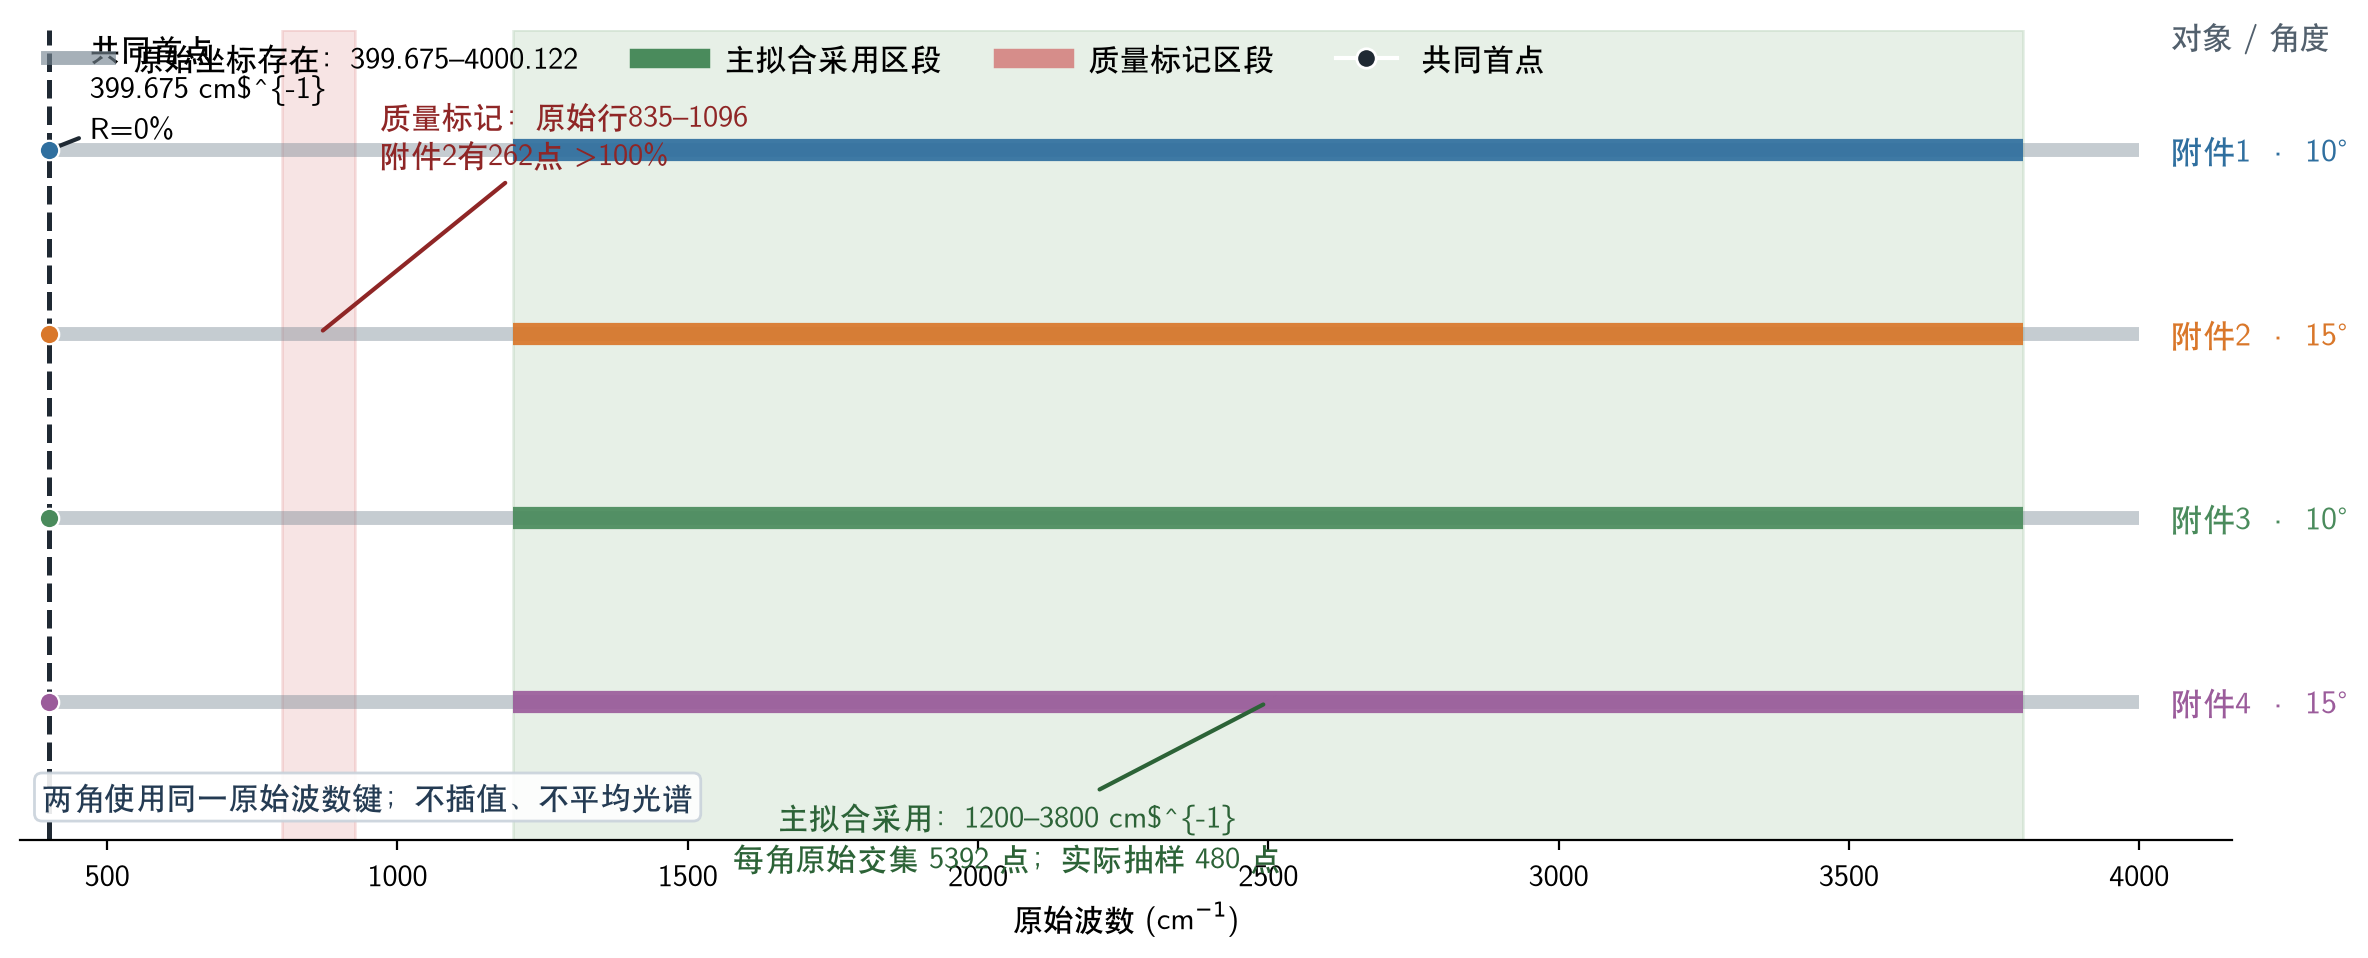
\includegraphics[width=0.8\textwidth]{../求解/公共/图片/共同坐标标记质量区段.png}
    \caption{四谱共同波数坐标及拟合区段}
    \label{fig:common-coordinate}
\end{figure}

抽样点集与全量点集承担不同任务：前者使各路线在同一组连续区段上比较，后者用于硅的主窗口整体拟合。共同抽样的480个点可由式\eqref{eq:supp-source-row}逐点回到工作表行号，而不是只知道所在波段。
% src:求解/问题2/结果/数据审查.json:抽样点数_每角度;抽样索引

\begin{equation}
\ell_j=1663+\left\lfloor\frac{5391j}{479}\right\rfloor,
\qquad j=0,\ldots,479.
\label{eq:supp-source-row}
\end{equation}
% src:求解/问题2/结果/数据审查.json:抽样索引;共同窗口原始点数_每角度;抽样点数_每角度
其中，$j$为从零起算的共同抽样序号，$\ell_j$为包含表头的源工作表行号，$\lfloor\cdot\rfloor$表示向下取整。同一序号在四个附件中对应相同波数，但反射率仍分别取各自原值；原始波段、角度和行号确定后，路线优劣才有共同的比较对象。

\subsubsection{路线比较：合成回收与实测预测分列}

路线比较先区分是否知道真实厚度。早期曾考虑直接用观测光谱衡量测厚误差，但附件缺少厚度真值和折射率曲线，因而改在原始共同坐标上构造24例已知光学条件的合成光谱；这一实际取舍决定了图\ref{fig:08}和表\ref{tab:04}中的误差衡量方法回收能力，而实测留段误差衡量谱形预测。
% src:交接/实验记录.json:22.尝试;22.现象;22.决定
% src:求解/问题1/结果/合成验证.json:分组汇总.共同匹配.案例数

双束界面场反演在原型共同案例上的平均相对误差为$0.0010\%$，正式共同匹配组为$0.0008\%$。表\ref{tab:supp-q1-routes}保留两个阶段的数值而不相互替换；新增匹配与故意改变光学关系的情景也单列，避免把匹配条件下的回收表现说成所有情景下的测厚精度。
% src:求解/问题1/原型结果/路线2.json:核心指标.合成厚度平均相对误差_百分比
% src:求解/问题1/结果/合成验证.json:主指标.数值

\begingroup
\small
\begin{longtable}{>{\centering\arraybackslash}p{0.18\textwidth}>{\centering\arraybackslash}p{0.30\textwidth}>{\centering\arraybackslash}p{0.14\textwidth}>{\centering\arraybackslash}p{0.26\textwidth}}
\caption{问题一原型与正式合成误差}\label{tab:supp-q1-routes}\\
\toprule
数据阶段 & 方法或情景 & 案例数 & 平均误差（\%） \\
\midrule
\endfirsthead
\toprule
数据阶段 & 方法或情景 & 案例数 & 平均误差（\%） \\
\midrule
\endhead
原型合成 & 色散峰序反演 & 24 & 0.0201 \\
原型合成 & 双束界面场反演 & 24 & 0.0010 \\
原型合成 & 连续相位拟厚 & 24 & 0.0041 \\
正式合成 & 共同匹配 & 24 & 0.0008 \\
正式合成 & 新增匹配 & 16 & 0.0011 \\
正式合成 & 模型失配 & 10 & 0.3028 \\
正式合成 & 常折射率峰距 & 24 & 2.5875 \\
\bottomrule
\end{longtable}
\endgroup
% src:求解/问题1/原型结果/路线1.json:主指标值;参数情景.组合数
% src:求解/问题1/原型结果/路线2.json:核心指标.合成厚度平均相对误差_百分比
% src:求解/问题1/原型结果/路线3.json:主指标值
% src:求解/问题1/结果/合成验证.json:分组汇总;常折射率峰距基线

模型失配组改变的是生成观测的光学关系，而非删除困难案例后重新计分；因此它回答的是模型假设改变时的误差增长。原型与正式共同组虽然同属已知光学条件比较，含噪观测和估计步骤均有所不同，应按阶段各自对照。

碳化硅正式留段误差为$1.2074$，二次趋势对照为$1.4404$，均为无量纲谱形误差。这里的标准化误差，是每块反射率误差除以该折该角训练残差的四分位距，再对测试块等权平均；四分位距表示训练残差中间一半的散布宽度。表\ref{tab:supp-q2-routes}保留三条原型路线与正式对照，表\ref{tab:supp-q2-prototype-thickness}另列原型厚度，防止把较小的谱形误差直接写成较小的厚度真值误差。
% src:求解/问题2/结果/验证.json:正式主方法分数_连续留段标准化均方根误差;正式二次趋势基线分数_连续留段标准化均方根误差;主指标含义

\begingroup
\small
\begin{longtable}{>{\centering\arraybackslash}p{0.28\textwidth}>{\centering\arraybackslash}p{0.14\textwidth}>{\centering\arraybackslash}p{0.14\textwidth}>{\centering\arraybackslash}p{0.14\textwidth}>{\centering\arraybackslash}p{0.14\textwidth}}
\caption{碳化硅三路线及正式谱形对照}\label{tab:supp-q2-routes}\\
\toprule
路线或阶段 & 总体误差 & 首折误差 & 次折误差 & 覆盖（\%） \\
\midrule
\endfirsthead
\toprule
路线或阶段 & 总体误差 & 首折误差 & 次折误差 & 覆盖（\%） \\
\midrule
\endhead
双角色散变投影 & 1.1717 & 0.7662 & 1.5772 & 49.06 \\
双角峰序匹配 & 1.2354 & 0.7319 & 1.7389 & 55.31 \\
双角相位回归 & 1.2202 & 0.7906 & 1.6498 & 53.75 \\
正式主方法 & 1.2074 & --- & --- & 49.06 \\
正式二次趋势 & 1.4404 & --- & --- & --- \\
正式训练均值 & 3.1578 & --- & --- & --- \\
\bottomrule
\end{longtable}
\endgroup
% src:交接/锦标赛_问题2.json:路线.0.实测指标;路线.1.实测指标;路线.2.实测指标
% src:求解/问题2/结果/验证.json:连续留段标准化均方根误差;基线对比
% src:求解/问题2/结果/区间覆盖.json:测试经验覆盖率

折间接近只描述当前切分下的表现。早期的双角色散变投影在两折间相差约$1.90\%$，随后将连续留段扩为五折时，厚度的相对极差达到$76.04\%$；因此保留原型候选，同时用更充分的切分比较解释正式厚度范围为何变宽。
% src:交接/实验记录.json:499.尝试;499.现象;499.决定;520.现象;520.决定
% src:求解/问题2/结果/验证.json:五折跨切分稳定性.相对极差

\begingroup
\small
\begin{longtable}{>{\centering\arraybackslash}p{0.28\textwidth}>{\centering\arraybackslash}p{0.20\textwidth}>{\centering\arraybackslash}p{0.20\textwidth}>{\centering\arraybackslash}p{0.20\textwidth}}
\caption{碳化硅原型路线的折间厚度差异}\label{tab:supp-q2-prototype-thickness}\\
\toprule
原型路线 & 首折（$\mu\mathrm m$） & 次折（$\mu\mathrm m$） & 相对极差（\%） \\
\midrule
\endfirsthead
\toprule
原型路线 & 首折（$\mu\mathrm m$） & 次折（$\mu\mathrm m$） & 相对极差（\%） \\
\midrule
\endhead
双角色散变投影 & 5.1710 & 5.0737 & 1.90 \\
双角峰序匹配 & 4.2978 & 15.0358 & 111.08 \\
双角相位回归 & 5.1109 & 3.9952 & 24.51 \\
\bottomrule
\end{longtable}
\endgroup
% src:交接/锦标赛_问题2.json:路线.0.实测指标;路线.1.实测指标;路线.2.实测指标

改变数据表达方式后，改善率也必须与本路线的基线成对使用。全谱稳健特征变体相对自身二次趋势改善$26.00\%$，其留段误差却高于所选路线；表\ref{tab:supp-q2-variants}同时保留方法误差和各自基线，避免以不同分母的改善率直接排序。
% src:求解/问题2/升格2/结果/验证.json:正式主方法相对正式二次趋势改善_百分比;正式主方法分数_连续留段标准化均方根误差
% src:求解/问题2/结果/验证.json:正式主方法分数_连续留段标准化均方根误差

\begingroup
\small
\begin{longtable}{>{\centering\arraybackslash}p{0.28\textwidth}>{\centering\arraybackslash}p{0.20\textwidth}>{\centering\arraybackslash}p{0.20\textwidth}>{\centering\arraybackslash}p{0.20\textwidth}}
\caption{碳化硅变体与各自基线的成对比较}\label{tab:supp-q2-variants}\\
\toprule
计算条件 & 方法误差 & 自身基线误差 & 改善（\%） \\
\midrule
\endfirsthead
\toprule
计算条件 & 方法误差 & 自身基线误差 & 改善（\%） \\
\midrule
\endhead
所选双角路线 & 1.2074 & 1.4404 & 16.17 \\
共同峰序变体 & 2.9711 & 2.7618 & -7.58 \\
全谱稳健特征 & 1.2500 & 1.6892 & 26.00 \\
全点相位耦合 & 1.9911 & 0.6281 & -216.98 \\
\bottomrule
\end{longtable}
\endgroup
% src:求解/问题2/结果/验证.json:正式主方法分数_连续留段标准化均方根误差;正式二次趋势基线分数_连续留段标准化均方根误差;正式主方法相对正式二次趋势改善_百分比
% src:求解/问题2/升格1/结果/验证.json:正式主方法分数_连续留段标准化均方根误差;正式二次趋势基线分数_连续留段标准化均方根误差;正式主方法相对正式二次趋势改善_百分比
% src:求解/问题2/升格2/结果/验证.json:正式主方法分数_连续留段标准化均方根误差;正式二次趋势基线分数_连续留段标准化均方根误差;正式主方法相对正式二次趋势改善_百分比
% src:求解/问题2/升格3/结果/验证.json:正式主方法分数_连续留段标准化均方根误差;正式二次趋势基线分数_连续留段标准化均方根误差;正式主方法相对正式二次趋势改善_百分比

全谱稳健特征和全点相位耦合改变了观测表达或响应约束，属于替代计算条件；负改善则明确表示方法误差高于自己的基线。它们保留为选型证据，不替换同一套正式点集上的比较。

往返衰减场反演在问题三原型中的总体误差为$1.1366$，但硅分项相对自身两束对照反而增大$2.24\%$。这项真实尝试促使材料分项单列：表\ref{tab:supp-q3-routes}保存三种方法的原型指标，正式检验再逐块检查收益方向。
% src:求解/问题3/原型结果/路线1.json:核心指标.连续留段标准化均方根误差
% src:交接/实验记录.json:70.尝试;70.现象;70.决定

\begingroup
\small
\begin{longtable}{>{\centering\arraybackslash}p{0.28\textwidth}>{\centering\arraybackslash}p{0.14\textwidth}>{\centering\arraybackslash}p{0.14\textwidth}>{\centering\arraybackslash}p{0.14\textwidth}>{\centering\arraybackslash}p{0.14\textwidth}}
\caption{问题三原型方法的分材料误差}\label{tab:supp-q3-routes}\\
\toprule
原型方法 & 总体误差 & 硅误差 & 碳化硅误差 & 覆盖（\%） \\
\midrule
\endfirsthead
\toprule
原型方法 & 总体误差 & 硅误差 & 碳化硅误差 & 覆盖（\%） \\
\midrule
\endhead
往返衰减场反演 & 1.1366 & 1.5194 & 0.7538 & 65.31 \\
共享相位谐波反演 & 2.6394 & 4.0070 & 1.2718 & 64.06 \\
周期形状配准 & 2.2638 & 3.3372 & 1.1904 & 76.09 \\
\bottomrule
\end{longtable}
\endgroup
% src:交接/锦标赛_问题3.json:路线.0.实测指标;路线.1.实测指标;路线.2.实测指标

周期形状配准能形成有限数值，但其训练区段对重复相位的支持较弱；形状预测与界面往返机制因此分开解释。所有原型数值均留在比较中，正式结论则继续由共同测试点上的物理模型对照承担。

完整场的总体标准化误差为$1.0231$，高于两束的$0.9812$；表\ref{tab:supp-q3-formal}将共同起点、相同预算的两模型与训练均值、二次趋势并列。纯场差须在同一光学参数下计算，重新估参的厚度差则另行比较。
% src:求解/问题3/结果/回炉轮3候选/仲裁闭环/20260910_131501_81623_建模公式/厚度结果.json:分材料验证.硅.逐折汇总.0.平均标准化均方根误差;分材料验证.硅.逐折汇总.1.平均标准化均方根误差;分材料验证.碳化硅.逐折汇总.0.平均标准化均方根误差;分材料验证.碳化硅.逐折汇总.1.平均标准化均方根误差

\begingroup
\small
\begin{longtable}{>{\centering\arraybackslash}p{0.32\textwidth}>{\centering\arraybackslash}p{0.30\textwidth}>{\centering\arraybackslash}p{0.30\textwidth}}
\caption{问题三正式共同测试点的误差}\label{tab:supp-q3-formal}\\
\toprule
比较方法 & 标准化误差 & 样本类别 \\
\midrule
\endfirsthead
\toprule
比较方法 & 标准化误差 & 样本类别 \\
\midrule
\endhead
完整往返 & 1.0231 & 正式实测 \\
两束截断 & 0.9812 & 正式实测 \\
训练均值 & 2.1929 & 正式实测 \\
二次趋势 & 1.4434 & 正式实测 \\
\bottomrule
\end{longtable}
\endgroup
% src:求解/问题3/结果/回炉轮3候选/仲裁闭环/20260910_131501_81623_建模公式/厚度结果.json:分材料验证.硅.逐折汇总.0.平均标准化均方根误差.两束;分材料验证.硅.逐折汇总.0.平均标准化均方根误差.完整往返;分材料验证.硅.逐折汇总.0.平均标准化均方根误差.训练均值;分材料验证.硅.逐折汇总.0.平均标准化均方根误差.二次趋势;分材料验证.硅.逐折汇总.1.平均标准化均方根误差.两束;分材料验证.硅.逐折汇总.1.平均标准化均方根误差.完整往返;分材料验证.硅.逐折汇总.1.平均标准化均方根误差.训练均值;分材料验证.硅.逐折汇总.1.平均标准化均方根误差.二次趋势;分材料验证.碳化硅.逐折汇总.0.平均标准化均方根误差.两束;分材料验证.碳化硅.逐折汇总.0.平均标准化均方根误差.完整往返;分材料验证.碳化硅.逐折汇总.0.平均标准化均方根误差.训练均值;分材料验证.碳化硅.逐折汇总.0.平均标准化均方根误差.二次趋势;分材料验证.碳化硅.逐折汇总.1.平均标准化均方根误差.两束;分材料验证.碳化硅.逐折汇总.1.平均标准化均方根误差.完整往返;分材料验证.碳化硅.逐折汇总.1.平均标准化均方根误差.训练均值;分材料验证.碳化硅.逐折汇总.1.平均标准化均方根误差.二次趋势

训练均值和二次趋势给出不解释干涉条纹的参照；两束截断则保留首轮返回，因此更直接检验高阶返回的增量。总体分数明确后，逐例与逐块记录继续揭示平均数中被掩盖的歧义和方向变化。

\subsubsection{逐块比较：保留角度差异与失效案例}

平均误差可能掩盖局部方向相反的区段。这里把合成相位歧义、碳化硅的切分变化和硅的逐块误差分别列出，检验对象始终与各自的观测点集对应。

连续相位拟厚在共同合成案例中有1例相位歧义，仍计入全部24例的平均误差。表\ref{tab:supp-q1-cases}保存原型逐例结果，低于显示精度的误差用上界表示，不将困难案例从均值中移除。
% src:求解/问题1/原型结果/路线3.json:辅助诊断.有歧义案例数;合成逐例
% src:交接/实验记录.json:58.尝试;58.现象;58.决定

\begingroup
\small
\begin{longtable}{>{\centering\arraybackslash}p{0.10\textwidth}>{\centering\arraybackslash}p{0.22\textwidth}>{\centering\arraybackslash}p{0.17\textwidth}>{\centering\arraybackslash}p{0.18\textwidth}>{\centering\arraybackslash}p{0.17\textwidth}}
\caption{共同合成案例的逐例相对误差}\label{tab:supp-q1-cases}\\
\toprule
案例 & 真厚度（$\mu\mathrm m$） & 峰序（\%） & 界面场（\%） & 相位（\%） \\
\midrule
\endfirsthead
\toprule
案例 & 真厚度（$\mu\mathrm m$） & 峰序（\%） & 界面场（\%） & 相位（\%） \\
\midrule
\endhead
1 & 3 & $<0.0001$ & $<0.0001$ & 0.0002 \\
2 & 3 & 0.2030 & 0.0050 & 0.0114 \\
3 & 3 & 0.0124 & $<0.0001$ & 0.0006 \\
4 & 3 & 0.0883 & 0.0027 & 0.0134 \\
5 & 3 & $<0.0001$ & $<0.0001$ & 0.0001 \\
6 & 3 & 0.0532 & 0.0046 & 0.0508 \\
7 & 3 & $<0.0001$ & $<0.0001$ & 0.0003 \\
8 & 3 & 0.0983 & 0.0044 & 0.0056 \\
9 & 8 & $<0.0001$ & $<0.0001$ & $<0.0001$ \\
10 & 8 & 0.0021 & 0.0021 & 0.0098 \\
11 & 8 & 0.0007 & $<0.0001$ & $<0.0001$ \\
12 & 8 & 0.0106 & 0.0009 & 0.0012 \\
13 & 8 & $<0.0001$ & $<0.0001$ & $<0.0001$ \\
14 & 8 & 0.0037 & 0.0012 & 0.0023 \\
15 & 8 & $<0.0001$ & $<0.0001$ & $<0.0001$ \\
16 & 8 & 0.0078 & 0.0015 & 0.0006 \\
17 & 20 & 0.0001 & $<0.0001$ & $<0.0001$ \\
18 & 20 & 0.0004 & 0.0004 & 0.0003 \\
19 & 20 & 0.0002 & $<0.0001$ & $<0.0001$ \\
20 & 20 & 0.0003 & $<0.0001$ & 0.0002 \\
21 & 20 & 0.0004 & $<0.0001$ & $<0.0001$ \\
22 & 20 & 0.0009 & 0.0002 & 0.0012 \\
23 & 20 & 0.0001 & $<0.0001$ & $<0.0001$ \\
24 & 20 & $<0.0001$ & 0.0005 & 0.0003 \\
\bottomrule
\end{longtable}
\endgroup
% src:求解/问题1/原型结果/路线1.json:逐例结果;参数情景
% src:求解/问题1/原型结果/路线2.json:逐例结果
% src:求解/问题1/原型结果/路线3.json:合成逐例

歧义案例的主候选为$3.0000\ \mu\mathrm m$，另一个近优候选为$36.8799\ \mu\mathrm m$。主候选接近真值与候选是否唯一是不同问题；保留这对候选，才能解释为何低平均误差仍需相位识别检查。
% src:求解/问题1/原型结果/路线3.json:合成逐例.0.求解.近优候选厚度_微米

碳化硅五折厚度横跨$5.5322$--$13.5109\ \mu\mathrm m$，表\ref{tab:supp-q2-folds}列出各折测试块与谱形误差；图\ref{fig:q2-angle}则从冻结另一角的光学参数检验共享厚度。切段和换角作用于不同的信息来源，因此两者分别保留。
% src:求解/问题2/结果/验证.json:五折跨切分稳定性.最小厚度_微米;五折跨切分稳定性.最大厚度_微米;五折连续留段

\begingroup
\small
\begin{longtable}{>{\centering\arraybackslash}p{0.14\textwidth}>{\centering\arraybackslash}p{0.22\textwidth}>{\centering\arraybackslash}p{0.26\textwidth}>{\centering\arraybackslash}p{0.26\textwidth}}
\caption{碳化硅五折厚度及留段误差}\label{tab:supp-q2-folds}\\
\toprule
折号 & 测试块号 & 厚度（$\mu\mathrm m$） & 标准化误差 \\
\midrule
\endfirsthead
\toprule
折号 & 测试块号 & 厚度（$\mu\mathrm m$） & 标准化误差 \\
\midrule
\endhead
1 & 1、2 & 13.3683 & 1.9693 \\
2 & 3、4 & 10.4926 & 0.6847 \\
3 & 5、6 & 6.5335 & 0.3407 \\
4 & 7、8 & 13.5109 & 0.4882 \\
5 & 9、10 & 5.5322 & 1.2048 \\
\bottomrule
\end{longtable}
\endgroup
% src:求解/问题2/结果/验证.json:五折连续留段;五折跨切分稳定性

五折搜索均取得有效参数，但换一段连续光谱，最合适的厚度分支仍会移动。这种变化解释了共同厚度约束的作用边界：它要求两角共用物理量，却不能凭空补齐未知的折射率曲线。

\begin{figure}[!htb]
  \centering
  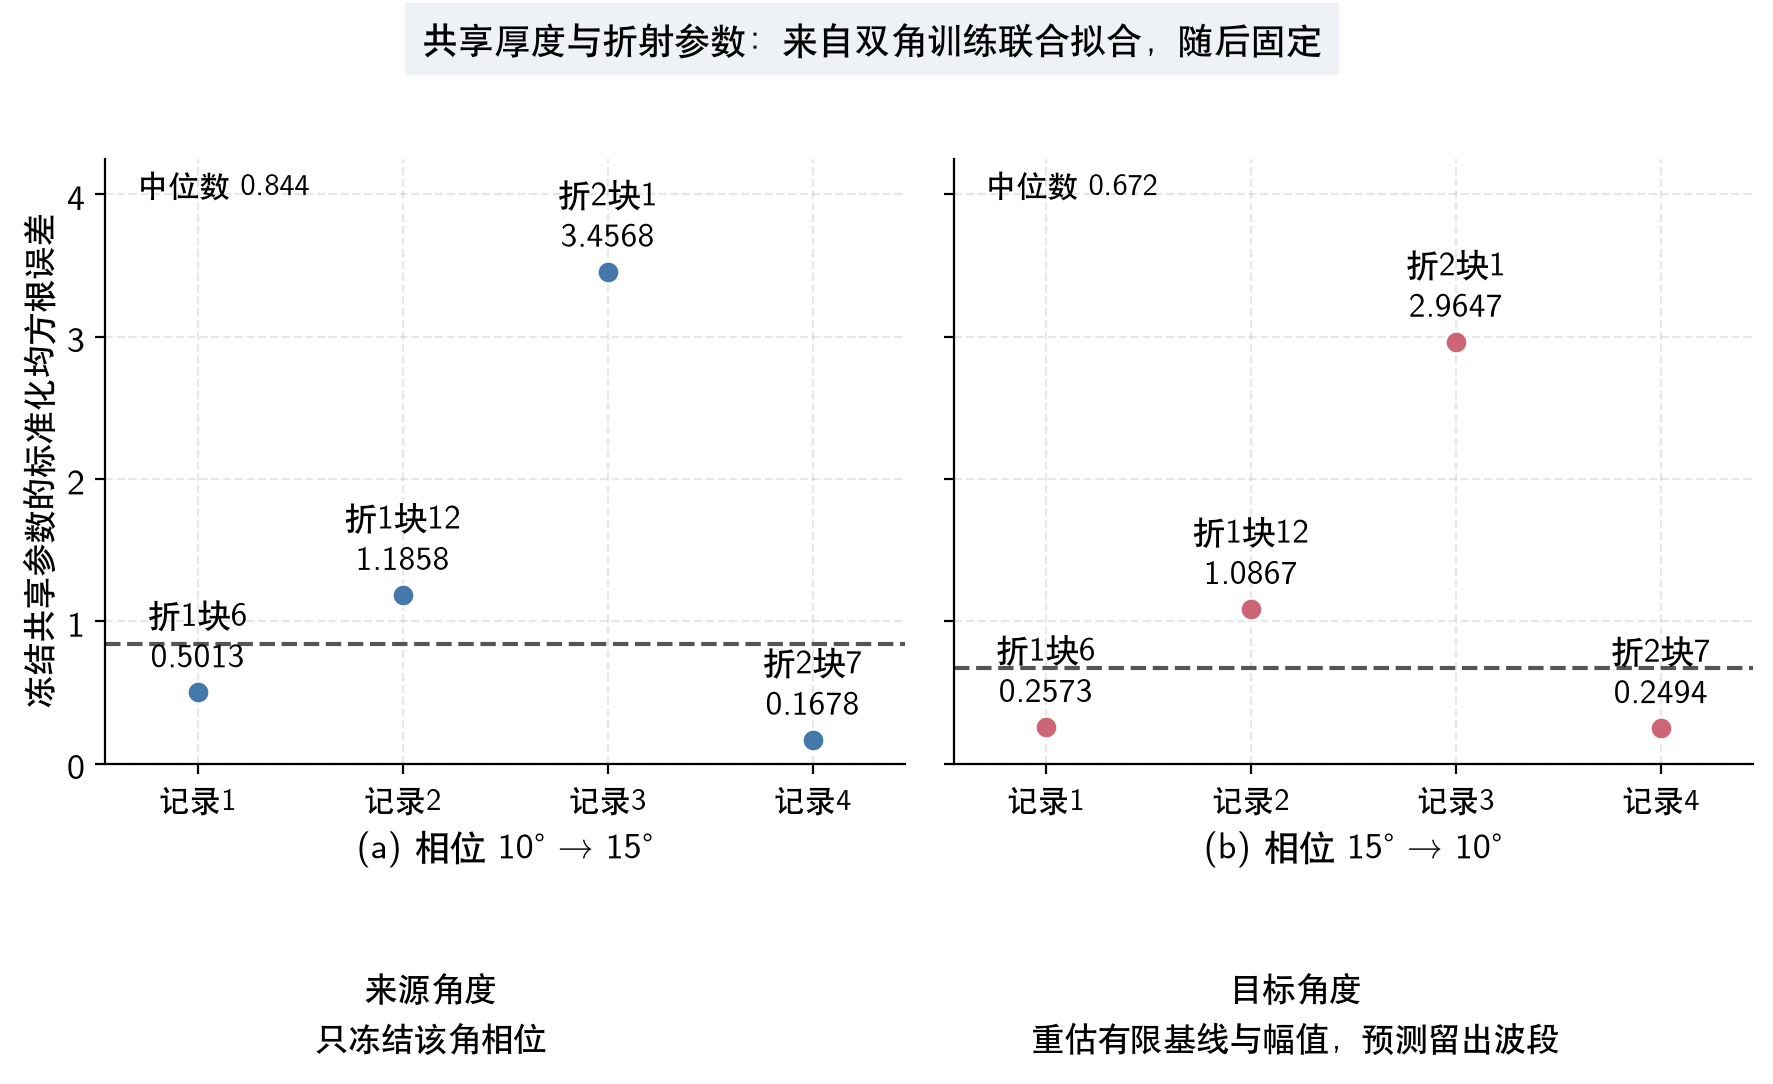
\includegraphics[width=0.8\textwidth]{../求解/问题2/图片/留角度预测核对共享厚度.png}
  \caption{双角参数固定后的跨角响应核对}
  \label{fig:q2-angle}
\end{figure}

完整场的总体误差为$1.0231$，高于两束的$0.9812$；表\ref{tab:supp-q3-blocks}逐块列出同一参数搜索设置下的差值，并与图\ref{fig:17}区分数值核对和图形展示。差值统一取两束误差减完整场误差，正值表示完整场在该块的预测误差较低。
% src:求解/问题3/结果/回炉轮3候选/仲裁闭环/20260910_131501_81623_建模公式/厚度结果.json:分材料验证.硅.逐折汇总.0.平均标准化均方根误差.两束;分材料验证.硅.逐折汇总.0.平均标准化均方根误差.完整往返;分材料验证.硅.逐折汇总.0.平均标准化均方根误差.训练均值;分材料验证.硅.逐折汇总.0.平均标准化均方根误差.二次趋势;分材料验证.硅.逐折汇总.1.平均标准化均方根误差.两束;分材料验证.硅.逐折汇总.1.平均标准化均方根误差.完整往返;分材料验证.硅.逐折汇总.1.平均标准化均方根误差.训练均值;分材料验证.硅.逐折汇总.1.平均标准化均方根误差.二次趋势;分材料验证.碳化硅.逐折汇总.0.平均标准化均方根误差.两束;分材料验证.碳化硅.逐折汇总.0.平均标准化均方根误差.完整往返;分材料验证.碳化硅.逐折汇总.0.平均标准化均方根误差.训练均值;分材料验证.碳化硅.逐折汇总.0.平均标准化均方根误差.二次趋势;分材料验证.碳化硅.逐折汇总.1.平均标准化均方根误差.两束;分材料验证.碳化硅.逐折汇总.1.平均标准化均方根误差.完整往返;分材料验证.碳化硅.逐折汇总.1.平均标准化均方根误差.训练均值;分材料验证.碳化硅.逐折汇总.1.平均标准化均方根误差.二次趋势
% src:交接/实验记录.json:563.尝试;563.现象;563.决定

\begingroup
\small
\setlength{\LTpre}{0pt}
\setlength{\LTpost}{0pt}
\renewcommand{\arraystretch}{1.00}
\begin{longtable}{>{\centering\arraybackslash}p{0.10\textwidth}>{\centering\arraybackslash}p{0.10\textwidth}>{\centering\arraybackslash}p{0.10\textwidth}>{\centering\arraybackslash}p{0.17\textwidth}>{\centering\arraybackslash}p{0.17\textwidth}>{\centering\arraybackslash}p{0.16\textwidth}}
\caption{全部测试块的完整往返与两束误差}\label{tab:supp-q3-blocks}\\
\toprule
附件 & 折号 & 块号 & 两束误差 & 完整往返 & 误差差值 \\
\midrule
\endfirsthead
\caption[]{全部测试块的完整往返与两束误差（续）}\\
\toprule
附件 & 折号 & 块号 & 两束误差 & 完整往返 & 误差差值 \\
\midrule
\endhead
1 & 1 & 6 & 0.1290 & 0.1287 & +0.0003 \\
1 & 1 & 12 & 0.1455 & 0.1460 & -0.0005 \\
1 & 2 & 1 & 2.0936 & 2.1254 & -0.0319 \\
1 & 2 & 7 & 0.1299 & 0.1251 & +0.0048 \\
2 & 1 & 6 & 0.3561 & 0.3504 & +0.0057 \\
2 & 1 & 12 & 0.2853 & 0.2860 & -0.0007 \\
2 & 2 & 1 & 2.4656 & 2.4803 & -0.0147 \\
2 & 2 & 7 & 0.2059 & 0.2013 & +0.0046 \\
3 & 1 & 6 & 0.1401 & 0.0982 & +0.0419 \\
3 & 1 & 12 & 0.2461 & 0.1861 & +0.0600 \\
3 & 2 & 1 & 4.1345 & 4.5085 & -0.3740 \\
3 & 2 & 7 & 0.3344 & 0.3937 & -0.0592 \\
4 & 1 & 6 & 0.3136 & 0.2514 & +0.0621 \\
4 & 1 & 12 & 0.1677 & 0.1115 & +0.0563 \\
4 & 2 & 1 & 4.4083 & 4.7480 & -0.3397 \\
4 & 2 & 7 & 0.1433 & 0.2289 & -0.0856 \\
\bottomrule
\end{longtable}
\endgroup
% src:求解/问题3/结果/回炉轮3候选/仲裁闭环/20260910_131501_81623_建模公式/厚度结果.json:逐块评分.32.标准化均方根误差;逐块评分.36.标准化均方根误差;逐块评分.33.标准化均方根误差;逐块评分.37.标准化均方根误差;逐块评分.48.标准化均方根误差;逐块评分.52.标准化均方根误差;逐块评分.49.标准化均方根误差;逐块评分.53.标准化均方根误差;逐块评分.34.标准化均方根误差;逐块评分.38.标准化均方根误差;逐块评分.35.标准化均方根误差;逐块评分.39.标准化均方根误差;逐块评分.50.标准化均方根误差;逐块评分.54.标准化均方根误差;逐块评分.51.标准化均方根误差;逐块评分.55.标准化均方根误差;逐块评分.0.标准化均方根误差;逐块评分.4.标准化均方根误差;逐块评分.1.标准化均方根误差;逐块评分.5.标准化均方根误差;逐块评分.16.标准化均方根误差;逐块评分.20.标准化均方根误差;逐块评分.17.标准化均方根误差;逐块评分.21.标准化均方根误差;逐块评分.2.标准化均方根误差;逐块评分.6.标准化均方根误差;逐块评分.3.标准化均方根误差;逐块评分.7.标准化均方根误差;逐块评分.18.标准化均方根误差;逐块评分.22.标准化均方根误差;逐块评分.19.标准化均方根误差;逐块评分.23.标准化均方根误差

负差值同时出现在硅与碳化硅，材料、角度和区段都会改变比较方向。上述差值衡量反射率预测，对应表\ref{tab:08}的两材料厚度处理，但不将局部拟合改善直接换算为厚度精度提升。

相位歧义、参考折射率边界和重复相位支持不足，各自对应不同的失败原因。表\ref{tab:supp-failures}连同硅原型的反向收益保存实际记录；其中曾把参考折射率减小$3\%$与触及物理边界后的取值混为一谈，后来将严格扰动和边界情景分开，避免用另一种条件冒充原先的扰动。
% src:交接/实验记录.json:519.尝试;519.现象;519.决定

\begingroup
\small
\begin{longtable}{>{\centering\arraybackslash}p{0.22\textwidth}>{\centering\arraybackslash}p{0.22\textwidth}>{\centering\arraybackslash}p{0.22\textwidth}>{\centering\arraybackslash}p{0.22\textwidth}}
\caption{实际尝试中的歧义与失效记录}\label{tab:supp-failures}\\
\toprule
尝试对象 & 实际现象 & 保留内容 & 解释方式 \\
\midrule
\endfirsthead
\toprule
尝试对象 & 实际现象 & 保留内容 & 解释方式 \\
\midrule
\endhead
合成相位路线 & 近优厚度不唯一 & 保留全部案例 & 候选成对列出 \\
实测折射率扰动 & 请求值越过边界 & 严格与边界分开 & 边界不并入范围 \\
原型周期形状 & 重复相位支持弱 & 保留有限数值 & 形状与机理分开 \\
原型硅往返场 & 分材料收益反向 & 保留硅误差 & 逐块比较方向 \\
\bottomrule
\end{longtable}
\endgroup
% src:求解/问题1/原型结果/路线3.json:辅助诊断.有歧义案例数;合成逐例.0.求解
% src:交接/实验记录.json:58.现象;58.决定;519.现象;519.决定;70.现象;70.决定
% src:求解/问题3/原型结果/锦标赛核验.json:路线三资格诊断;路线核验.0.分材料

这些记录区分了“算出数值”与“识别唯一厚度”两件事，也保留了复杂路线局部变差的证据。路线和失效对象明确后，区间检验进一步核对预测带实际容纳了多少观测。

\subsubsection{区间计数：反射率覆盖与厚度范围分开}

反射率区间检查的是未参与拟合和校准的观测值是否落在预测带内；厚度范围则记录切分与光学条件改变后的取值。两类量分别保存分子、分母和参与比较的对象，以便回查表\ref{tab:09}和表\ref{tab:10}。

碳化硅正式反射率测试共有320点，其中157点落入预测带，经验覆盖率为$49.06\%$；图\ref{fig:q2-coverage}给出局部覆盖形态，表\ref{tab:supp-coverage}补全分角度计数。预测带的半宽取校准块绝对残差的固定经验分位，覆盖率则由测试块另行计算。
% src:求解/问题2/结果/区间覆盖.json:测试点数;测试经验覆盖率;构造方法
% src:求解/问题2/结果/验证.json:分块

问题二实际采用$75\%$校准分位；问题三采用$90\%$校准分位。前者没有设定名义覆盖保证，因此两问覆盖率既要结合各自的预测带构造解释，也要保持反射率与厚度这两类对象的区分。
% src:求解/问题2/结果/区间覆盖.json:校准经验分位点;构造方法
% src:求解/问题3/结果/回炉轮3候选/仲裁闭环/20260910_131501_81623_建模公式/厚度结果.json:预测区间.4.经验覆盖率;预测区间.4.平均区间宽度_比例;预测区间.5.经验覆盖率;预测区间.5.平均区间宽度_比例;预测区间.6.经验覆盖率;预测区间.6.平均区间宽度_比例;预测区间.7.经验覆盖率;预测区间.7.平均区间宽度_比例;预测区间.20.经验覆盖率;预测区间.20.平均区间宽度_比例;预测区间.21.经验覆盖率;预测区间.21.平均区间宽度_比例;预测区间.22.经验覆盖率;预测区间.22.平均区间宽度_比例;预测区间.23.经验覆盖率;预测区间.23.平均区间宽度_比例;预测区间.36.经验覆盖率;预测区间.36.平均区间宽度_比例;预测区间.37.经验覆盖率;预测区间.37.平均区间宽度_比例;预测区间.38.经验覆盖率;预测区间.38.平均区间宽度_比例;预测区间.39.经验覆盖率;预测区间.39.平均区间宽度_比例;预测区间.52.经验覆盖率;预测区间.52.平均区间宽度_比例;预测区间.53.经验覆盖率;预测区间.53.平均区间宽度_比例;预测区间.54.经验覆盖率;预测区间.54.平均区间宽度_比例;预测区间.55.经验覆盖率;预测区间.55.平均区间宽度_比例;预测区间.4.名义覆盖率
% src:求解/问题3/结果/回炉轮3候选/仲裁闭环/20260910_131501_81623_建模公式/厚度结果.json:逐块评分.4.测试点数;逐块评分.5.测试点数;逐块评分.6.测试点数;逐块评分.7.测试点数;逐块评分.20.测试点数;逐块评分.21.测试点数;逐块评分.22.测试点数;逐块评分.23.测试点数;逐块评分.36.测试点数;逐块评分.37.测试点数;逐块评分.38.测试点数;逐块评分.39.测试点数;逐块评分.52.测试点数;逐块评分.53.测试点数;逐块评分.54.测试点数;逐块评分.55.测试点数

完整往返的反射率测试共有640点，其中473点被预测带覆盖，经验覆盖率为$73.91\%$。表\ref{tab:supp-coverage}按材料与角度拆开这个总数，避免把某一材料较宽的预测带当成所有观测都得到同等解释。
% src:求解/问题3/结果/回炉轮3候选/仲裁闭环/20260910_131501_81623_建模公式/厚度结果.json:预测区间.4.经验覆盖率;预测区间.4.平均区间宽度_比例;预测区间.5.经验覆盖率;预测区间.5.平均区间宽度_比例;预测区间.6.经验覆盖率;预测区间.6.平均区间宽度_比例;预测区间.7.经验覆盖率;预测区间.7.平均区间宽度_比例;预测区间.20.经验覆盖率;预测区间.20.平均区间宽度_比例;预测区间.21.经验覆盖率;预测区间.21.平均区间宽度_比例;预测区间.22.经验覆盖率;预测区间.22.平均区间宽度_比例;预测区间.23.经验覆盖率;预测区间.23.平均区间宽度_比例;预测区间.36.经验覆盖率;预测区间.36.平均区间宽度_比例;预测区间.37.经验覆盖率;预测区间.37.平均区间宽度_比例;预测区间.38.经验覆盖率;预测区间.38.平均区间宽度_比例;预测区间.39.经验覆盖率;预测区间.39.平均区间宽度_比例;预测区间.52.经验覆盖率;预测区间.52.平均区间宽度_比例;预测区间.53.经验覆盖率;预测区间.53.平均区间宽度_比例;预测区间.54.经验覆盖率;预测区间.54.平均区间宽度_比例;预测区间.55.经验覆盖率;预测区间.55.平均区间宽度_比例;预测区间.4.名义覆盖率
% src:求解/问题3/结果/回炉轮3候选/仲裁闭环/20260910_131501_81623_建模公式/厚度结果.json:逐块评分.4.测试点数;逐块评分.5.测试点数;逐块评分.6.测试点数;逐块评分.7.测试点数;逐块评分.20.测试点数;逐块评分.21.测试点数;逐块评分.22.测试点数;逐块评分.23.测试点数;逐块评分.36.测试点数;逐块评分.37.测试点数;逐块评分.38.测试点数;逐块评分.39.测试点数;逐块评分.52.测试点数;逐块评分.53.测试点数;逐块评分.54.测试点数;逐块评分.55.测试点数

\begingroup
\small
\begin{longtable}{>{\centering\arraybackslash}p{0.12\textwidth}>{\centering\arraybackslash}p{0.14\textwidth}>{\centering\arraybackslash}p{0.12\textwidth}>{\centering\arraybackslash}p{0.14\textwidth}>{\centering\arraybackslash}p{0.14\textwidth}>{\centering\arraybackslash}p{0.14\textwidth}}
\caption{反射率测试覆盖的分材料分角计数}\label{tab:supp-coverage}\\
\toprule
问题 & 材料 & 角度 & 覆盖点 & 测试点 & 覆盖（\%） \\
\midrule
\endfirsthead
\toprule
问题 & 材料 & 角度 & 覆盖点 & 测试点 & 覆盖（\%） \\
\midrule
\endhead
问题三 & 硅 & $10^\circ$ & 119 & 160 & 74.38 \\
问题三 & 硅 & $15^\circ$ & 123 & 160 & 76.88 \\
问题三 & 碳化硅 & $10^\circ$ & 132 & 160 & 82.50 \\
问题三 & 碳化硅 & $15^\circ$ & 99 & 160 & 61.88 \\
问题二 & 碳化硅 & $10^\circ$ & 84 & 160 & 52.50 \\
问题二 & 碳化硅 & $15^\circ$ & 73 & 160 & 45.63 \\
问题二 & 合计 & --- & 157 & 320 & 49.06 \\
问题三 & 合计 & --- & 473 & 640 & 73.91 \\
\bottomrule
\end{longtable}
\endgroup
% src:求解/问题2/结果/验证.json:分块
% src:求解/问题2/结果/区间覆盖.json:测试经验覆盖率;测试点数
% src:求解/问题3/结果/回炉轮3候选/仲裁闭环/20260910_131501_81623_建模公式/厚度结果.json:逐块评分.32.标准化均方根误差;逐块评分.36.标准化均方根误差;逐块评分.33.标准化均方根误差;逐块评分.37.标准化均方根误差;逐块评分.48.标准化均方根误差;逐块评分.52.标准化均方根误差;逐块评分.49.标准化均方根误差;逐块评分.53.标准化均方根误差;逐块评分.34.标准化均方根误差;逐块评分.38.标准化均方根误差;逐块评分.35.标准化均方根误差;逐块评分.39.标准化均方根误差;逐块评分.50.标准化均方根误差;逐块评分.54.标准化均方根误差;逐块评分.51.标准化均方根误差;逐块评分.55.标准化均方根误差;逐块评分.0.标准化均方根误差;逐块评分.4.标准化均方根误差;逐块评分.1.标准化均方根误差;逐块评分.5.标准化均方根误差;逐块评分.16.标准化均方根误差;逐块评分.20.标准化均方根误差;逐块评分.17.标准化均方根误差;逐块评分.21.标准化均方根误差;逐块评分.2.标准化均方根误差;逐块评分.6.标准化均方根误差;逐块评分.3.标准化均方根误差;逐块评分.7.标准化均方根误差;逐块评分.18.标准化均方根误差;逐块评分.22.标准化均方根误差;逐块评分.19.标准化均方根误差;逐块评分.23.标准化均方根误差
% src:求解/问题3/结果/回炉轮3候选/仲裁闭环/20260910_131501_81623_建模公式/厚度结果.json:预测区间.4.经验覆盖率;预测区间.4.平均区间宽度_比例;预测区间.5.经验覆盖率;预测区间.5.平均区间宽度_比例;预测区间.6.经验覆盖率;预测区间.6.平均区间宽度_比例;预测区间.7.经验覆盖率;预测区间.7.平均区间宽度_比例;预测区间.20.经验覆盖率;预测区间.20.平均区间宽度_比例;预测区间.21.经验覆盖率;预测区间.21.平均区间宽度_比例;预测区间.22.经验覆盖率;预测区间.22.平均区间宽度_比例;预测区间.23.经验覆盖率;预测区间.23.平均区间宽度_比例;预测区间.36.经验覆盖率;预测区间.36.平均区间宽度_比例;预测区间.37.经验覆盖率;预测区间.37.平均区间宽度_比例;预测区间.38.经验覆盖率;预测区间.38.平均区间宽度_比例;预测区间.39.经验覆盖率;预测区间.39.平均区间宽度_比例;预测区间.52.经验覆盖率;预测区间.52.平均区间宽度_比例;预测区间.53.经验覆盖率;预测区间.53.平均区间宽度_比例;预测区间.54.经验覆盖率;预测区间.54.平均区间宽度_比例;预测区间.55.经验覆盖率;预测区间.55.平均区间宽度_比例;预测区间.4.名义覆盖率
% src:求解/问题3/结果/回炉轮3候选/仲裁闭环/20260910_131501_81623_建模公式/厚度结果.json:逐块评分.4.测试点数;逐块评分.5.测试点数;逐块评分.6.测试点数;逐块评分.7.测试点数;逐块评分.20.测试点数;逐块评分.21.测试点数;逐块评分.22.测试点数;逐块评分.23.测试点数;逐块评分.36.测试点数;逐块评分.37.测试点数;逐块评分.38.测试点数;逐块评分.39.测试点数;逐块评分.52.测试点数;逐块评分.53.测试点数;逐块评分.54.测试点数;逐块评分.55.测试点数

这些分母统计的是连续测试块内的反射率观测，而非独立晶圆数。厚度随条件改变的范围不参与覆盖计数；它们在表\ref{tab:supp-range}中按形成方式另列，其中碳化硅的范围为$0.6367$--$18.1064\ \mu\mathrm m$，来自切分、光学剖面和合法参数情景的并集。
% src:求解/问题2/结果/厚度结果.json:条件区间_微米;条件区间组成;条件区间构造

\begingroup
\small
\begin{longtable}{>{\centering\arraybackslash}p{0.24\textwidth}>{\centering\arraybackslash}p{0.20\textwidth}>{\centering\arraybackslash}p{0.20\textwidth}>{\centering\arraybackslash}p{0.24\textwidth}}
\caption{厚度范围与形成对象分别对应}\label{tab:supp-range}\\
\toprule
对象 & 下限（$\mu\mathrm m$） & 上限（$\mu\mathrm m$） & 范围形成方式 \\
\midrule
\endfirsthead
\toprule
对象 & 下限（$\mu\mathrm m$） & 上限（$\mu\mathrm m$） & 范围形成方式 \\
\midrule
\endhead
问题一合成扰动 & 6.6622 & 10.0142 & 同一锚例重估 \\
问题二碳化硅 & 0.6367 & 18.1064 & 切分与情景并集 \\
问题三硅两折 & 1.7322 & 16.0424 & 连续留段折间范围 \\
问题三硅包络 & 1.7246 & 18.1553 & 非概率情景联合包络 \\
问题三碳化硅 & 0.6367 & 18.1064 & 沿用问题二基准 \\
\bottomrule
\end{longtable}
\endgroup
% src:求解/问题1/结果/灵敏度.json:条件压力范围_微米
% src:求解/问题2/结果/厚度结果.json:条件区间_微米;条件区间组成
% src:求解/问题3/结果/回炉轮3候选/仲裁闭环/20260910_131501_81623_建模公式/厚度结果.json:核心指标.硅折1完整往返条件厚度_um;核心指标.硅折2完整往返条件厚度_um;核心指标.碳化硅正式条件范围下限_um;核心指标.碳化硅正式条件范围上限_um

折间范围来自重估条件的变化，主窗口全量拟合则使用另一组观测对象：硅每角保留5392个原始点，给出的厚度为$2.1651\ \mu\mathrm m$。同段两束值为$2.3193\ \mu\mathrm m$，完整往返减两束为$-0.1542\ \mu\mathrm m$。
% src:求解/问题3/结果/回炉轮3候选/仲裁闭环/20260910_131501_81623_建模公式/厚度结果.json:案例.0.最优.厚度_um;案例.1.最优.厚度_um;案例.6.最优.厚度_um;案例.7.最优.厚度_um

硅两折相差$14.3102\ \mu\mathrm m$，完整包络为$1.7246$--$18.1553\ \mu\mathrm m$。全量值、两折跨度与包含近优候选和扰动的情景包络各有不同统计对象。
% src:求解/问题3/结果/回炉轮3候选/仲裁闭环/20260910_131501_81623_建模公式/厚度结果.json:核心指标.硅全量完整往返厚度_um;核心指标.硅折1完整往返条件厚度_um;核心指标.硅折2完整往返条件厚度_um;核心指标.硅已计算条件包络下限_um;核心指标.硅已计算条件包络上限_um;核心指标.碳化硅正式基准厚度_um;核心指标.碳化硅正式条件范围下限_um;核心指标.碳化硅正式条件范围上限_um
% src:求解/问题3/结果/解读核验_回炉3_仲裁后.json:防泄漏.全量每角点数
% src:求解/问题3/结果/回炉轮3候选/仲裁闭环/20260910_131501_81623_建模公式/厚度结果.json:核心指标.硅全量完整往返厚度_um

历史窗口扰动保留原训练块成员并取窗口交集；表\ref{tab:supp-window-sensitivity}列出当时参与重估的训练点数与厚度，与图\ref{fig:19}的原参数扰动对象对应。点数是各折训练源行的数量，不再把整个切窗样本数写成实际训练点数；该历史表中的范围不代表本次条件包络端点。
% src:求解/问题3/结果/灵敏度.json:灵敏度_参数扰动
% src:交接/实验记录.json:564.尝试;564.现象;564.决定

\begin{figure}[!htb]
  \centering
  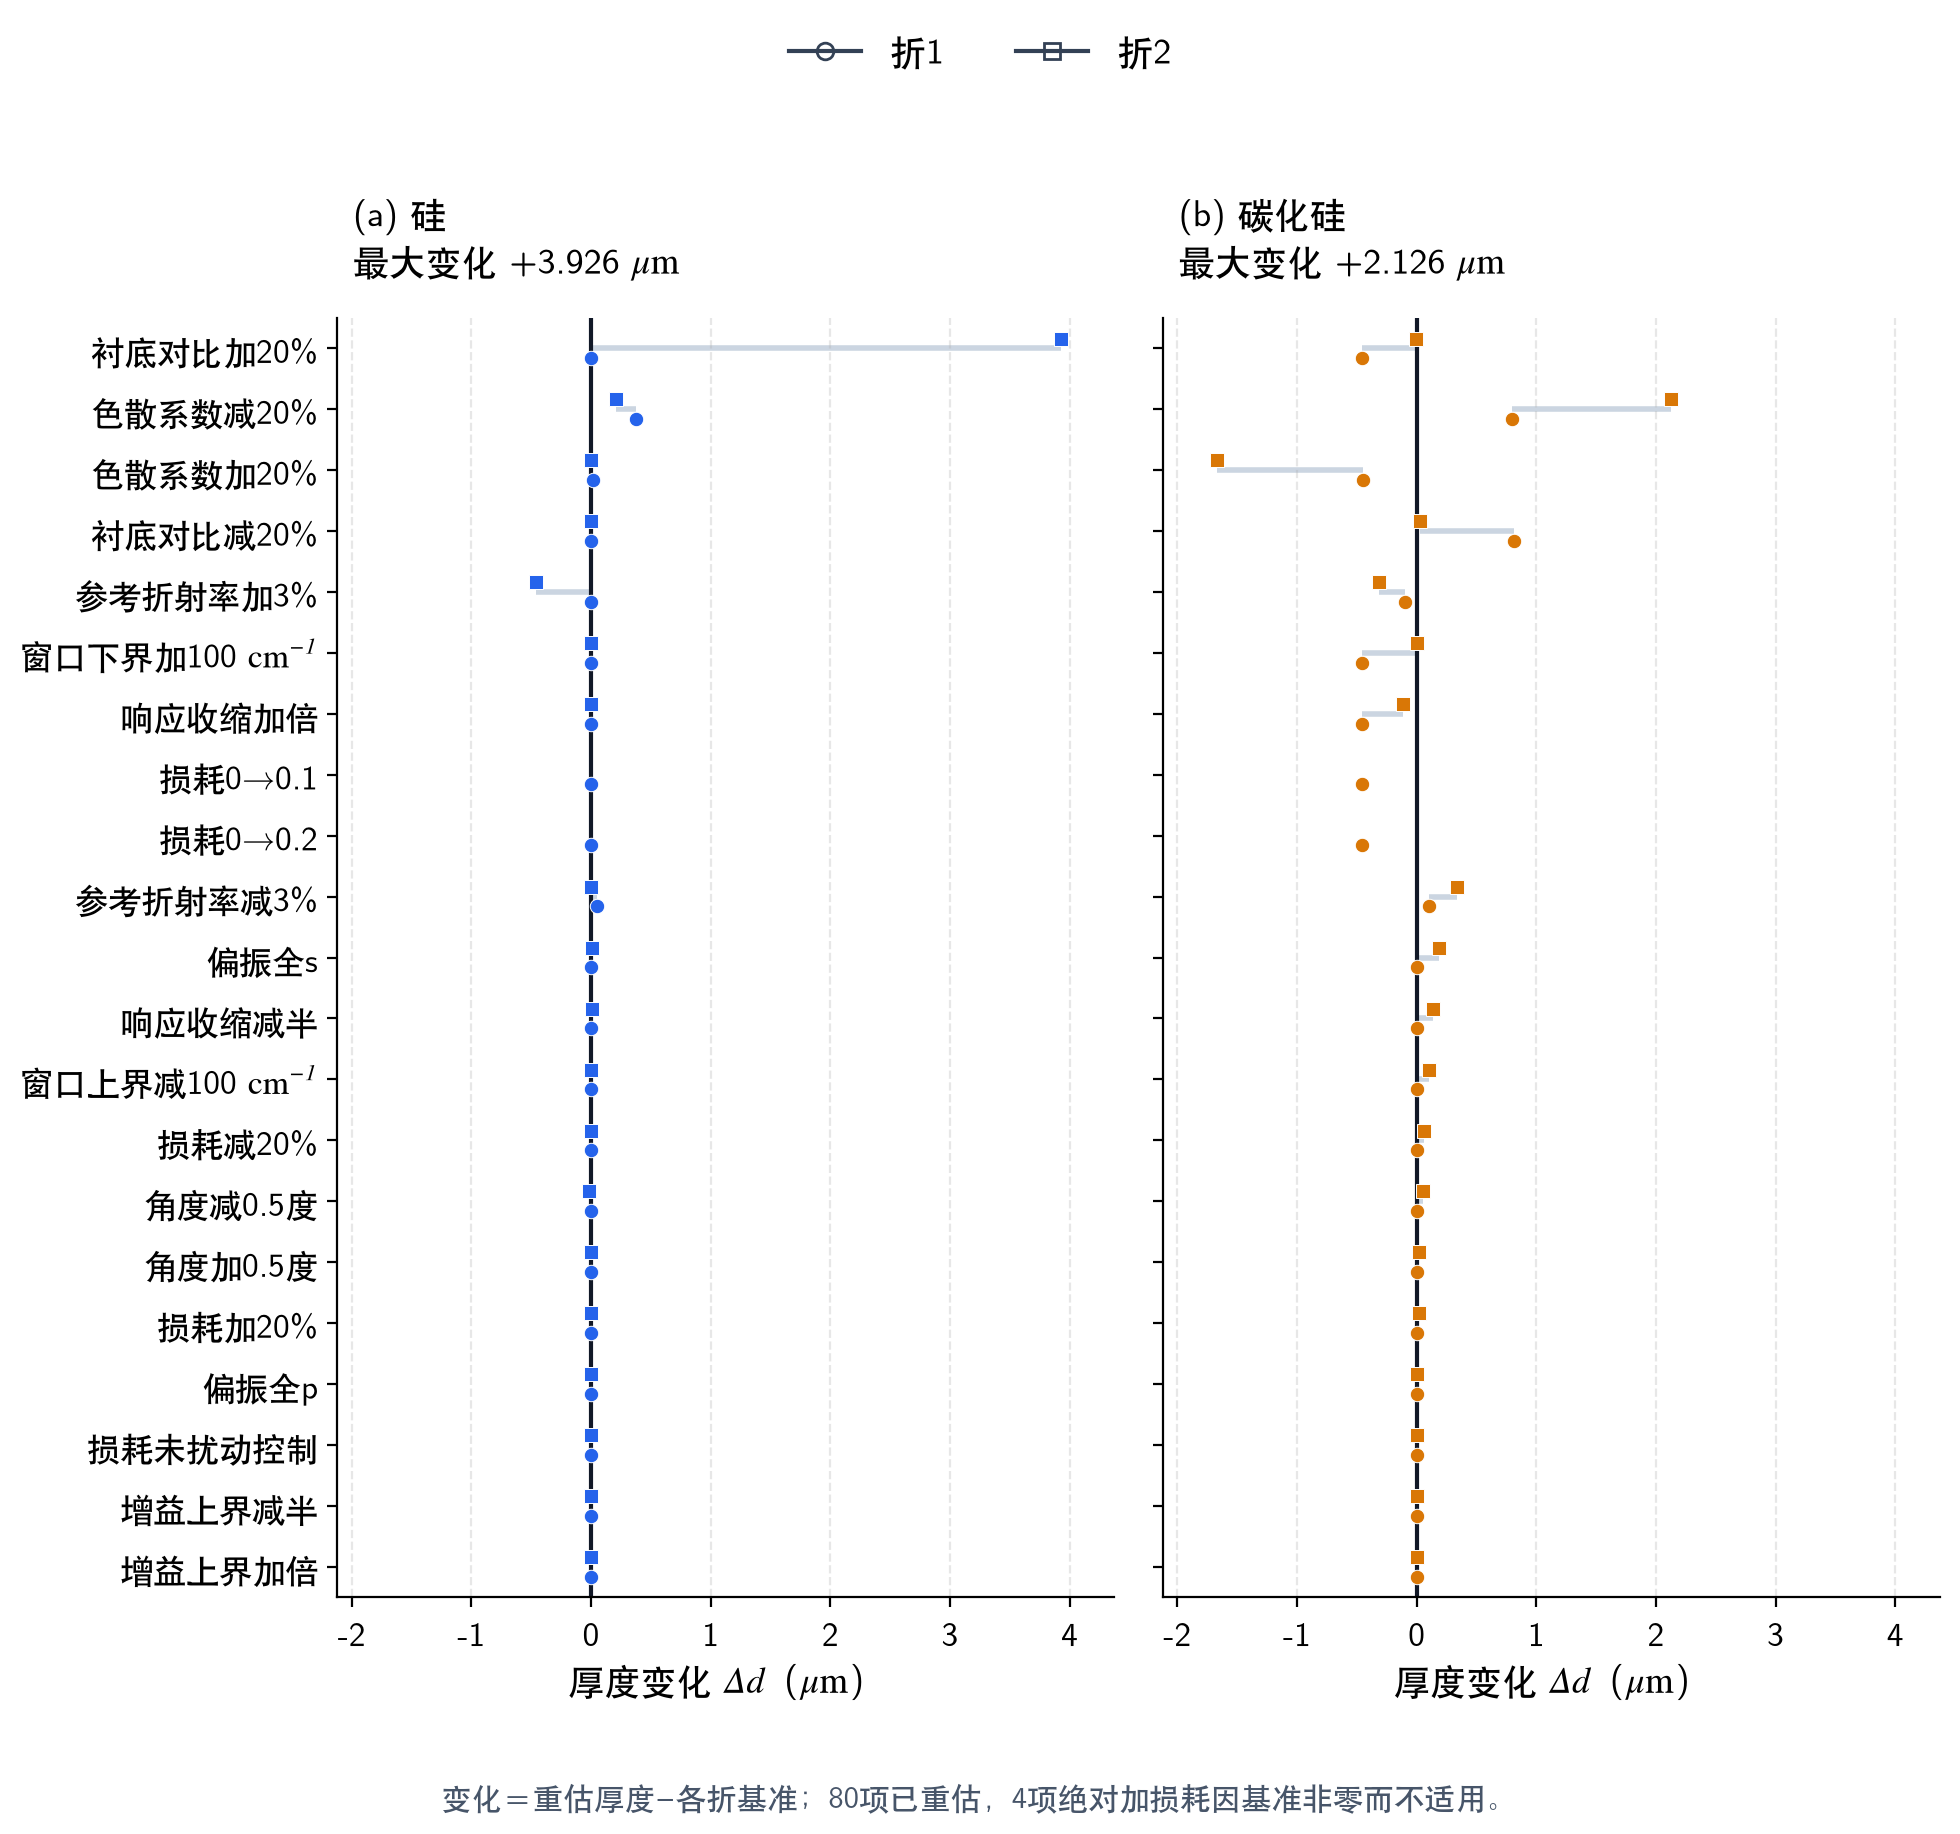
\includegraphics[width=0.8\textwidth]{../求解/问题3/图片/厚度扰动区分谱形与测厚影响.png}
  \caption{两材料厚度随参数扰动发生偏移}
  \label{fig:19}
\end{figure}

\begingroup
\small
\begin{longtable}{>{\centering\arraybackslash}p{0.14\textwidth}>{\centering\arraybackslash}p{0.08\textwidth}>{\centering\arraybackslash}p{0.26\textwidth}>{\centering\arraybackslash}p{0.12\textwidth}>{\centering\arraybackslash}p{0.24\textwidth}}
\caption{历史窗口扰动的点数与重估厚度}\label{tab:supp-window-sensitivity}\\
\toprule
材料 & 折号 & 窗口（$\mathrm{cm}^{-1}$） & 训练点数 & 厚度（$\mu\mathrm m$） \\
\midrule
\endfirsthead
\toprule
材料 & 折号 & 窗口（$\mathrm{cm}^{-1}$） & 训练点数 & 厚度（$\mu\mathrm m$） \\
\midrule
\endhead
硅 & 1 & 1300--3800 & 273 & 1.7345 \\
硅 & 1 & 1200--3700 & 292 & 1.7321 \\
硅 & 2 & 1300--3800 & 292 & 16.0426 \\
硅 & 2 & 1200--3700 & 273 & 16.0424 \\
碳化硅 & 1 & 1300--3800 & 273 & 2.7611 \\
碳化硅 & 1 & 1200--3700 & 292 & 3.2168 \\
碳化硅 & 2 & 1300--3800 & 292 & 10.6616 \\
碳化硅 & 2 & 1200--3700 & 273 & 10.7635 \\
\bottomrule
\end{longtable}
\endgroup
% src:求解/问题3/结果/灵敏度.json:灵敏度_参数扰动

下界内移时按原始波数筛选训练成员，未在端点外插观测。各折训练源行分别保留，窗口变化和区段切分据此具有明确的样本对象。
% src:求解/问题3/结果/灵敏度.json:灵敏度_参数扰动

上界内移采用同一交集规则；重估厚度对照未扰动的同折解，而不与另一折或全量拟合混合。
% src:求解/问题3/结果/灵敏度.json:灵敏度_参数扰动

历史参数与窗口对照共列84项情景，其中80项完成重估，4项因适用条件不满足而单列。表\ref{tab:supp-all-sensitivity}保留原材料和折次的厚度变化；这些差值相对于当时的同折完整往返解，区别于本次同起点控制差，碳化硅的往返对照与问题二采用值也分别承担不同任务。
% src:求解/问题3/结果/灵敏度.json:灵敏度_参数扰动

\begingroup
\small
\setlength{\LTpre}{0pt}
\setlength{\LTpost}{0pt}
\renewcommand{\arraystretch}{1.00}
\begin{longtable}{>{\centering\arraybackslash}p{0.28\textwidth}>{\centering\arraybackslash}p{0.14\textwidth}>{\centering\arraybackslash}p{0.14\textwidth}>{\centering\arraybackslash}p{0.14\textwidth}>{\centering\arraybackslash}p{0.14\textwidth}}
\caption{历史扰动的厚度变化量（微米）}\label{tab:supp-all-sensitivity}\\
\toprule
扰动情景 & 硅首折 & 硅次折 & 碳化硅首折 & 碳化硅次折 \\
\midrule
\endfirsthead
\caption[]{历史扰动的厚度变化量（微米，续）}\\
\toprule
扰动情景 & 硅首折 & 硅次折 & 碳化硅首折 & 碳化硅次折 \\
\midrule
\endhead
有效损耗未扰动控制 & +0.0000 & +0.0002 & +0.0000 & +0.0000 \\
有效损耗减20\% & +0.0000 & +0.0002 & +0.0000 & +0.0648 \\
有效损耗加20\% & +0.0000 & +0.0002 & +0.0000 & +0.0164 \\
有效损耗绝对增加$0\to$0.1 & +0.0003 & 不适用 & -0.4553 & 不适用 \\
有效损耗绝对增加$0\to$0.2 & +0.0006 & 不适用 & -0.4552 & 不适用 \\
衬底对比减20\% & +0.0006 & +0.0026 & +0.8142 & +0.0303 \\
衬底对比加20\% & +0.0000 & +3.9259 & -0.4552 & -0.0037 \\
参考折射率减3\% & +0.0535 & +0.0002 & +0.0997 & +0.3370 \\
参考折射率加3\% & +0.0000 & -0.4571 & -0.0939 & -0.3168 \\
色散系数减20\% & +0.3767 & +0.2068 & +0.7962 & +2.1261 \\
色散系数加20\% & +0.0152 & +0.0000 & -0.4521 & -1.6720 \\
偏振全$s$ & +0.0000 & +0.0063 & +0.0000 & +0.1841 \\
偏振全$p$ & +0.0000 & -0.0001 & -0.0002 & +0.0000 \\
入射角同时减0.5度 & -0.0001 & -0.0159 & -0.0002 & +0.0509 \\
入射角同时加0.5度 & +0.0001 & +0.0000 & +0.0000 & +0.0208 \\
窗口下界加100 & +0.0024 & +0.0002 & -0.4557 & +0.0000 \\
窗口上界减100 & +0.0000 & +0.0000 & +0.0000 & +0.1019 \\
响应收缩减半 & +0.0001 & +0.0064 & +0.0002 & +0.1342 \\
响应收缩加倍 & -0.0001 & +0.0002 & -0.4555 & -0.1147 \\
标准化增益上界减半 & +0.0000 & +0.0002 & +0.0000 & +0.0000 \\
标准化增益上界加倍 & +0.0000 & +0.0002 & +0.0000 & +0.0000 \\
\bottomrule
\end{longtable}
\endgroup
% src:求解/问题3/结果/灵敏度.json:灵敏度_参数扰动

扰动结果同时保留变大、变小与显示精度下不变的取值；它们记录特定光学条件附近的重估响应，而不是给观测增加独立重复次数。源附件、比较路线、失败原因、覆盖计数与有效点数至此逐一对应，正文的各项结论均可回到相同对象核查。

\begingroup
\setlength{\intextsep}{4pt plus 1pt minus 1pt}
\setlength{\textfloatsep}{4pt plus 1pt minus 1pt}
\subsubsection{补充图证：场展开与色散响应}

场展开的两种表达在图\ref{fig:field-expansion}中逐点对照，比较对象为合场强度与交叉项展开。

\begin{figure}[!htb]
  \centering
  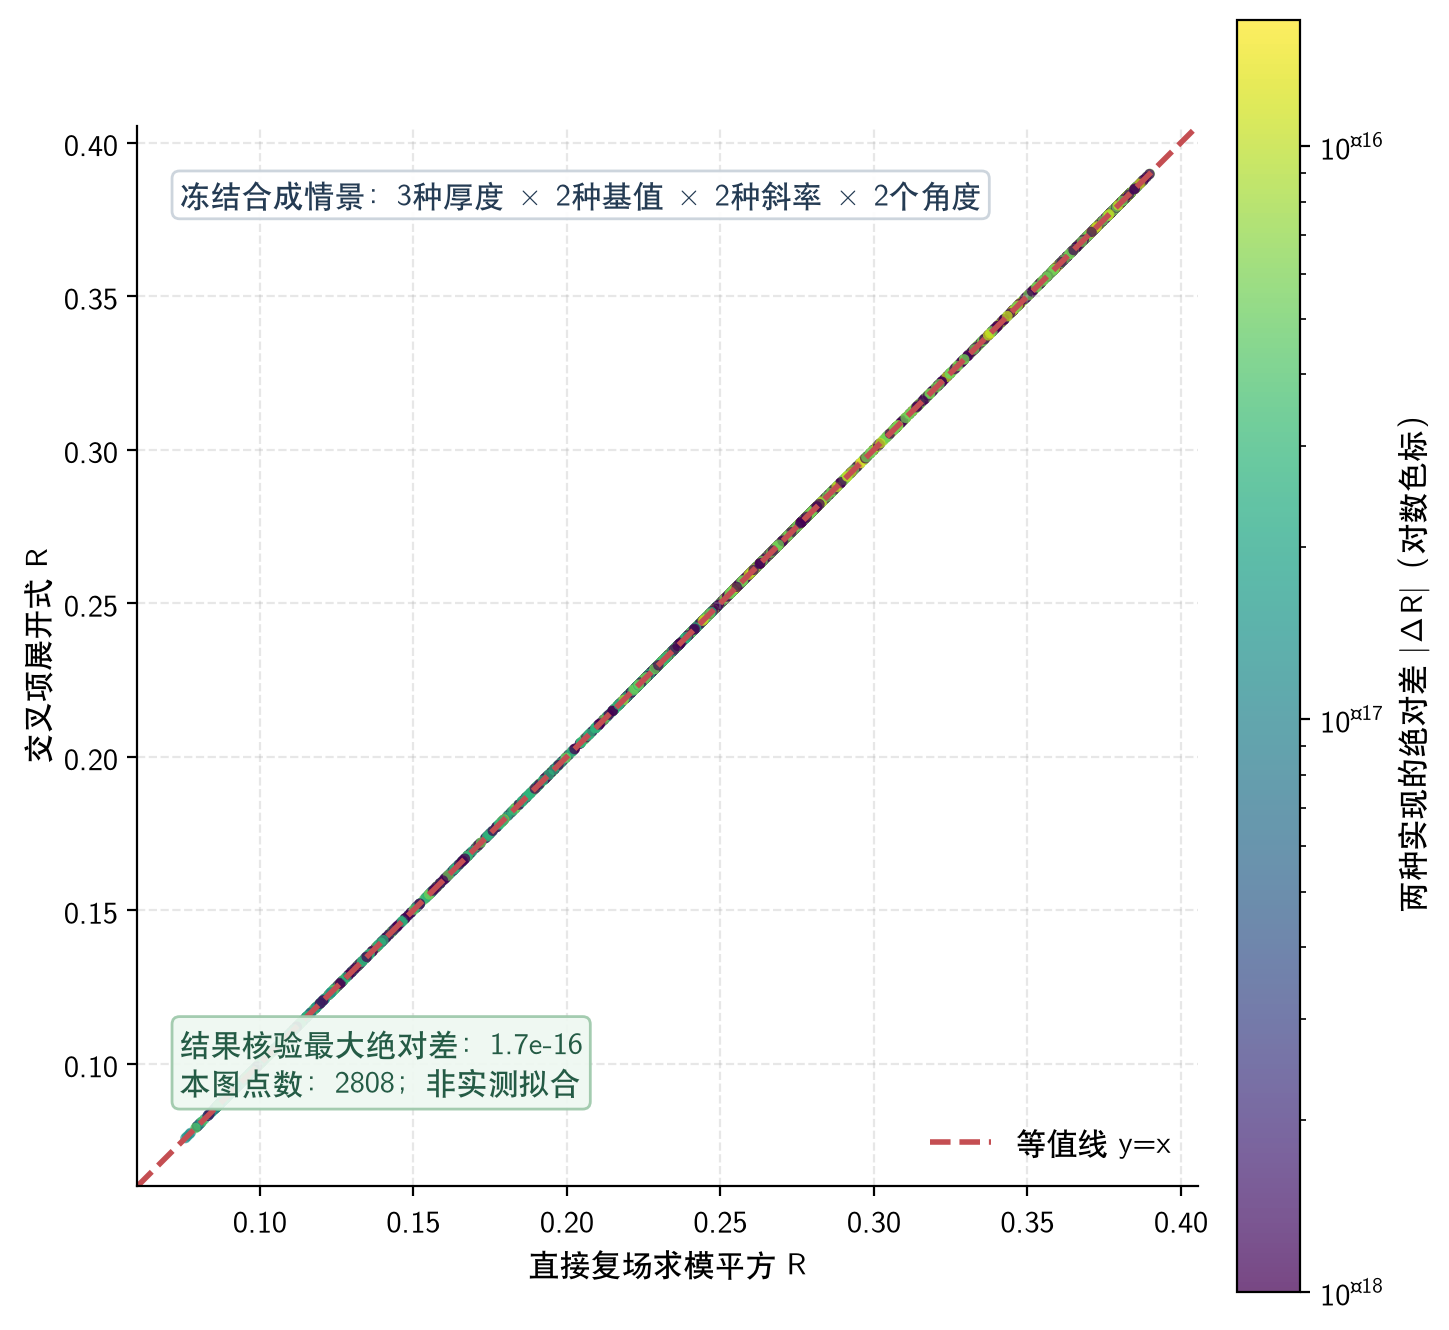
\includegraphics[width=0.8\textwidth]{../求解/问题1/图片/场求和与展开强度相符.png}
  \caption{两种强度展开实现的逐点一致性}
  \label{fig:field-expansion}
\end{figure}

图\ref{fig:dispersion-spacing}呈现折射变化对局部峰距的影响，与常折射率近似比较。

\begin{figure}[!htb]
  \centering
  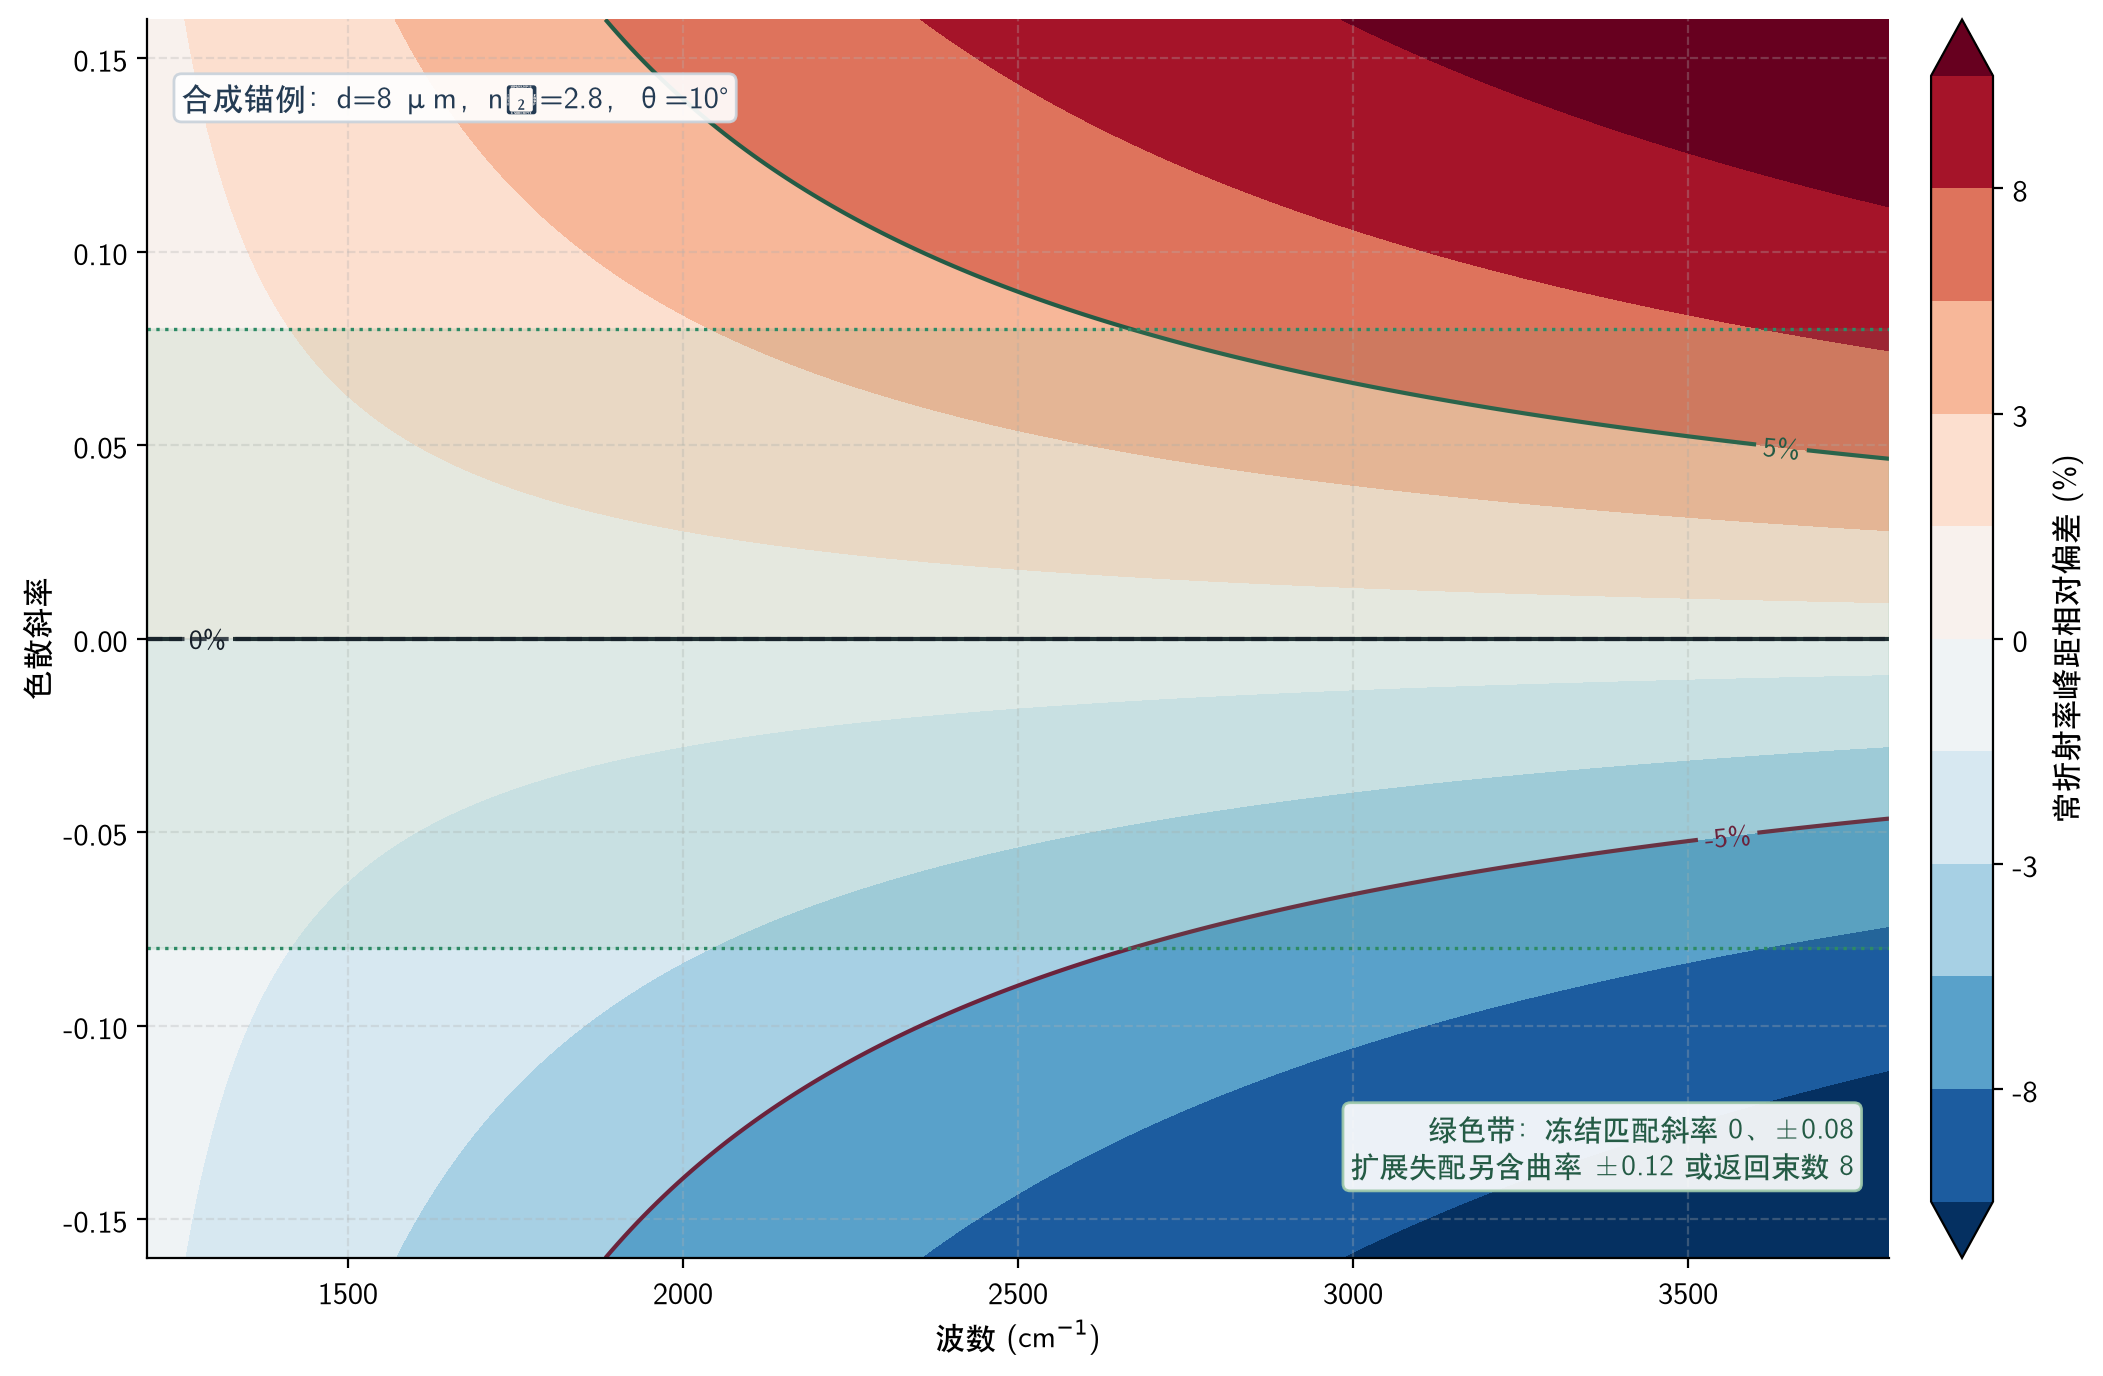
\includegraphics[width=0.8\textwidth]{../求解/问题1/图片/色散斜率改变局部峰距.png}
  \caption{色散斜率对局部峰距偏差的影响}
  \label{fig:dispersion-spacing}
\end{figure}
\endgroup

\end{document}
